% Measured, not estimated: what routing an agent to a cheaper model actually costs
% Build with `make` (runs build_assets.py, then latexmk -pdf).
\documentclass[11pt,letterpaper]{article}

% ---------------------------------------------------------------- fonts & page
\usepackage[T1]{fontenc}
\usepackage[utf8]{inputenc}
\usepackage{libertinus}
\usepackage[scaled=0.85]{beramono}
\usepackage[margin=0.9in,headheight=14pt]{geometry}
\usepackage{microtype}
\input{glyphtounicode}\pdfgentounicode=1 % real text in the PDF (copy, search, screen readers)
\usepackage{setspace}\setstretch{1.02}
\usepackage{parskip}
\usepackage{fancyhdr}
\pagestyle{fancy}\fancyhf{}
\fancyhead[L]{\small\itshape Paired measurement of routing costs}
\fancyhead[R]{\small\itshape October 2, 2026 (revised October 5, 2026)}
\fancyfoot[C]{\small\thepage}
\renewcommand{\headrulewidth}{0.3pt}

% ---------------------------------------------------------------- colours (Okabe-Ito)
\usepackage[table]{xcolor}
\definecolor{okblue}{HTML}{0072B2}
\definecolor{okorange}{HTML}{D55E00}
\definecolor{okgreen}{HTML}{009E73}
\definecolor{okgray}{HTML}{8A8A85}

% ---------------------------------------------------------------- tables, lists, maths
\usepackage{amsmath,amssymb}
\usepackage{booktabs,array,tabularx,xltabular,multirow}
\usepackage{graphicx}
\usepackage{pifont}
\usepackage[inline]{enumitem}
\setlist{itemsep=2pt,topsep=4pt}
\usepackage{siunitx}
\sisetup{group-separator={,},group-minimum-digits=4}
\usepackage{listings}
\lstset{basicstyle=\ttfamily\small,columns=fullflexible,keepspaces=true,frame=none,
        breaklines=true,aboveskip=2pt,belowskip=2pt,xleftmargin=1em}
\usepackage[font=small,labelfont=bf,skip=4pt]{caption}
\usepackage{float}

% ---------------------------------------------------------------- plots
\usepackage{pgfplots}
\usepackage{pgfplotstable}
\pgfplotsset{compat=1.18}
\usepgfplotslibrary{groupplots,statistics}
\usetikzlibrary{patterns,plotmarks,calc,arrows.meta,positioning,decorations.pathreplacing}
\tikzset{
  scatterlabel/.style={font=\scriptsize, inner sep=2pt, outer sep=0pt, fill=white, fill opacity=0.85, text opacity=1},
  scatterlabelmulti/.style={align=left, font=\scriptsize\linespread{1.15}\selectfont},
  leader/.style={okgray, line width=0.5pt},
}
\pgfplotsset{
  benchmark/.style={
    tick label style={font=\small}, label style={font=\small},
    legend style={font=\small, draw=okgray!60, fill=white, fill opacity=0.9, text opacity=1},
    grid style={okgray!25}, major grid style={okgray!25},
    axis line style={black!70}, every axis plot/.append style={line width=0.9pt},
  },
}

% ---------------------------------------------------------------- boxes
\usepackage[most]{tcolorbox}
\newtcolorbox{keyidea}[1][]{enhanced, breakable, colback=okblue!5, colframe=okblue,
  boxrule=0.6pt, arc=2pt, left=6pt, right=6pt, top=4pt, bottom=4pt,
  fonttitle=\bfseries\small, coltitle=white, title={Key idea}, #1}
\newtcolorbox{caution}[1][]{enhanced, breakable, colback=okorange!5, colframe=okorange,
  boxrule=0.6pt, arc=2pt, left=6pt, right=6pt, top=4pt, bottom=4pt,
  fonttitle=\bfseries\small, coltitle=white, title={Read with care}, #1}
\newtcolorbox{casecard}[1]{enhanced, breakable, colback=white, colframe=okgray,
  boxrule=0.5pt, arc=2pt, left=6pt, right=6pt, top=4pt, bottom=4pt,
  fonttitle=\bfseries\small, coltitle=black, colbacktitle=okgray!18, title={#1}}
\newcommand{\howtoread}[1]{\par\smallskip{\small\noindent\textbf{How to read this figure.} #1\par}}
\newcommand{\howtoreadtable}[1]{\par\smallskip{\small\noindent\textbf{How to read this table.} #1\par}}

% labels and symbols
\newcommand{\screen}{\textsf{\small\color{okgray}[screen]}}
\newcommand{\prereg}{\textsf{\small\color{okblue}[preregistered]}}
\newcommand{\ok}{\textcolor{okgreen}{\ding{51}}}
\newcommand{\no}{\textcolor{okorange}{\ding{55}}}
\newcommand{\symok}{\textcolor{okgreen}{\ding{51}}}
\newcommand{\symbad}{\textcolor{okorange}{\ding{55}}}
\newcommand{\symfb}{\textcolor{okgray}{$\curvearrowright$}}
\newcommand{\vconf}{\textcolor{okgreen}{\textsf{confirmed}}}
\newcommand{\vref}{\textcolor{okorange}{\textbf{\textsf{refuted}}}}
\newcommand{\vrev}{\textcolor{okblue}{\textsf{revised}}}
\newcommand{\vnew}{\textcolor{okgray}{\textsf{new}}}
\newcommand{\term}[1]{\emph{#1}}
\newcommand{\code}[1]{\texttt{#1}}
\newcommand{\pct}{\,\%}

% ---------------------------------------------------------------- numbers
% Generated by build_assets.py from docs/evidence/2026-10-02-paired-campaign/ and the files listed there. Do not edit.
% 1010 macros.
\newcommand{\AAAll}{1.007}
\newcommand{\AAAllCI}{0.97--1.04}
\newcommand{\AAAllCentred}{yes}
\newcommand{\AAAllN}{55}
\newcommand{\AAAllPct}{1}
\newcommand{\AAAllSD}{0.11}
\newcommand{\AAAllSDSession}{0.08}
\newcommand{\AABiasPct}{5}
\newcommand{\AAFable}{0.968}
\newcommand{\AAFableCI}{0.94--1.00}
\newcommand{\AAFableCentred}{yes}
\newcommand{\AAFableN}{28}
\newcommand{\AAFablePct}{3}
\newcommand{\AAFableSD}{0.10}
\newcommand{\AAFableSDSession}{0.07}
\newcommand{\AAOpus}{1.049}
\newcommand{\AAOpusCI}{1.01--1.09}
\newcommand{\AAOpusCentred}{no}
\newcommand{\AAOpusN}{27}
\newcommand{\AAOpusPct}{5}
\newcommand{\AAOpusSD}{0.10}
\newcommand{\AAOpusSDSession}{0.07}
\newcommand{\AAPct}{20}
\newcommand{\AuditFlagged}{0}
\newcommand{\BERawShippedForty}{1.03}
\newcommand{\BERawShippedThirty}{1.15}
\newcommand{\BERawShippedThirtyFive}{1.09}
\newcommand{\BERawSonnetForty}{1.12}
\newcommand{\BERawSonnetThirty}{1.26}
\newcommand{\BERawSonnetThirtyFive}{1.18}
\newcommand{\BERawStickyForty}{0.93}
\newcommand{\BERawStickyThirty}{1.04}
\newcommand{\BERawStickyThirtyFive}{0.98}
\newcommand{\BEReadMultiple}{1.90}
\newcommand{\BEShippedArm}{0.44}
\newcommand{\BEShippedPair}{0.49}
\newcommand{\BESonnetArm}{0.51}
\newcommand{\BESonnetPair}{0.50}
\newcommand{\BEStickyArm}{0.34}
\newcommand{\BEStickyForty}{0.98}
\newcommand{\BEStickyPair}{0.38}
\newcommand{\BEStickyThirty}{1.09}
\newcommand{\BEStickyThirtyFive}{1.03}
\newcommand{\Boot}{10{,}000}
\newcommand{\BootSeed}{20261002}
\newcommand{\BuildSha}{3aa2d1e}
\newcommand{\CacheTTLMin}{5}
\newcommand{\CfFableShippedArm}{0.618}
\newcommand{\CfFableShippedArmCI}{0.55--0.70}
\newcommand{\CfFableShippedArmCITwo}{0.55--0.70}
\newcommand{\CfFableShippedArmN}{46}
\newcommand{\CfFableShippedArmTwo}{0.62}
\newcommand{\CfFableShippedCents}{63}
\newcommand{\CfFableShippedExtra}{$-$37}
\newcommand{\CfFableShippedNValid}{46}
\newcommand{\CfFableShippedPair}{0.629}
\newcommand{\CfFableShippedPairCI}{0.56--0.71}
\newcommand{\CfFableShippedPairCITwo}{0.56--0.71}
\newcommand{\CfFableShippedPairN}{39}
\newcommand{\CfFableShippedPairTwo}{0.63}
\newcommand{\CfFableShippedSaving}{37}
\newcommand{\CfFableSonnetArm}{0.590}
\newcommand{\CfFableSonnetArmCI}{0.53--0.66}
\newcommand{\CfFableSonnetArmCITwo}{0.53--0.66}
\newcommand{\CfFableSonnetArmN}{46}
\newcommand{\CfFableSonnetArmTwo}{0.59}
\newcommand{\CfFableSonnetCents}{58}
\newcommand{\CfFableSonnetExtra}{$-$42}
\newcommand{\CfFableSonnetNValid}{46}
\newcommand{\CfFableSonnetPair}{0.577}
\newcommand{\CfFableSonnetPairCI}{0.52--0.65}
\newcommand{\CfFableSonnetPairCITwo}{0.52--0.65}
\newcommand{\CfFableSonnetPairN}{39}
\newcommand{\CfFableSonnetPairTwo}{0.58}
\newcommand{\CfFableSonnetSaving}{42}
\newcommand{\CfFableStickyArm}{0.537}
\newcommand{\CfFableStickyArmCI}{0.48--0.61}
\newcommand{\CfFableStickyArmCITwo}{0.48--0.61}
\newcommand{\CfFableStickyArmN}{46}
\newcommand{\CfFableStickyArmTwo}{0.54}
\newcommand{\CfFableStickyCents}{56}
\newcommand{\CfFableStickyExtra}{$-$44}
\newcommand{\CfFableStickyNValid}{46}
\newcommand{\CfFableStickyPair}{0.558}
\newcommand{\CfFableStickyPairCI}{0.49--0.64}
\newcommand{\CfFableStickyPairCITwo}{0.49--0.64}
\newcommand{\CfFableStickyPairN}{38}
\newcommand{\CfFableStickyPairTwo}{0.56}
\newcommand{\CfFableStickySaving}{44}
\newcommand{\CfOpusShippedArm}{1.321}
\newcommand{\CfOpusShippedArmCI}{1.19--1.46}
\newcommand{\CfOpusShippedArmCITwo}{1.19--1.46}
\newcommand{\CfOpusShippedArmExtra}{32}
\newcommand{\CfOpusShippedArmN}{46}
\newcommand{\CfOpusShippedArmTwo}{1.32}
\newcommand{\CfOpusShippedCents}{138}
\newcommand{\CfOpusShippedExtra}{38}
\newcommand{\CfOpusShippedNValid}{46}
\newcommand{\CfOpusShippedPair}{1.380}
\newcommand{\CfOpusShippedPairCI}{1.25--1.53}
\newcommand{\CfOpusShippedPairCITwo}{1.25--1.53}
\newcommand{\CfOpusShippedPairN}{38}
\newcommand{\CfOpusShippedPairTwo}{1.38}
\newcommand{\CfOpusShippedSaving}{$-$38}
\newcommand{\CfOpusSonnetArm}{1.457}
\newcommand{\CfOpusSonnetArmCI}{1.28--1.67}
\newcommand{\CfOpusSonnetArmCITwo}{1.28--1.67}
\newcommand{\CfOpusSonnetArmExtra}{46}
\newcommand{\CfOpusSonnetArmN}{46}
\newcommand{\CfOpusSonnetArmTwo}{1.46}
\newcommand{\CfOpusSonnetCents}{143}
\newcommand{\CfOpusSonnetExtra}{43}
\newcommand{\CfOpusSonnetNValid}{46}
\newcommand{\CfOpusSonnetPair}{1.433}
\newcommand{\CfOpusSonnetPairCI}{1.25--1.64}
\newcommand{\CfOpusSonnetPairCITwo}{1.25--1.64}
\newcommand{\CfOpusSonnetPairN}{40}
\newcommand{\CfOpusSonnetPairTwo}{1.43}
\newcommand{\CfOpusSonnetSaving}{$-$43}
\newcommand{\CfOpusStickyArm}{1.203}
\newcommand{\CfOpusStickyArmCI}{1.08--1.33}
\newcommand{\CfOpusStickyArmCITwo}{1.08--1.33}
\newcommand{\CfOpusStickyArmExtra}{20}
\newcommand{\CfOpusStickyArmN}{46}
\newcommand{\CfOpusStickyArmTwo}{1.20}
\newcommand{\CfOpusStickyCents}{125}
\newcommand{\CfOpusStickyExtra}{25}
\newcommand{\CfOpusStickyNValid}{46}
\newcommand{\CfOpusStickyPair}{1.249}
\newcommand{\CfOpusStickyPairCI}{1.13--1.39}
\newcommand{\CfOpusStickyPairCITwo}{1.13--1.39}
\newcommand{\CfOpusStickyPairN}{38}
\newcommand{\CfOpusStickyPairTwo}{1.25}
\newcommand{\CfOpusStickySaving}{$-$25}
\newcommand{\ClClefCostXHigh}{4.4}
\newcommand{\ClClefCostXLow}{3.2}
\newcommand{\ClClefPfiftyHigh}{429}
\newcommand{\ClClefPfiftyLow}{391}
\newcommand{\ClClefPninetyfiveHigh}{738}
\newcommand{\ClClefPninetyfiveLow}{663}
\newcommand{\ClClefPrice}{0.24}
\newcommand{\ClClefRequests}{1{,}296}
\newcommand{\ClClefSlow}{0}
\newcommand{\ClDevClefAcc}{85}
\newcommand{\ClDevClefAccCI}{88--98\,\%}
\newcommand{\ClDevClefAccPct}{94.4}
\newcommand{\ClDevClefCost}{51.4}
\newcommand{\ClDevClefCov}{69}
\newcommand{\ClDevClefFlashHolm}{0.043}
\newcommand{\ClDevClefJevHolm}{1.000}
\newcommand{\ClDevClefPfifty}{422}
\newcommand{\ClDevClefPninetyfive}{725}
\newcommand{\ClDevClefWa}{1}
\newcommand{\ClDevFlashAcc}{77}
\newcommand{\ClDevFlashAccCI}{77--91\,\%}
\newcommand{\ClDevFlashAccPct}{85.6}
\newcommand{\ClDevFlashCost}{19.3}
\newcommand{\ClDevFlashCov}{70}
\newcommand{\ClDevFlashJevHolm}{0.008}
\newcommand{\ClDevFlashPfifty}{321}
\newcommand{\ClDevFlashPninetyfive}{825}
\newcommand{\ClDevFlashWa}{7}
\newcommand{\ClDevJevAcc}{86}
\newcommand{\ClDevJevAccCI}{89--98\,\%}
\newcommand{\ClDevJevAccPct}{95.6}
\newcommand{\ClDevJevCost}{15.9}
\newcommand{\ClDevJevCov}{68}
\newcommand{\ClDevJevPfifty}{152}
\newcommand{\ClDevJevPninetyfive}{231}
\newcommand{\ClDevJevWa}{2}
\newcommand{\ClDevN}{90}
\newcommand{\ClFlashCostXHigh}{1.7}
\newcommand{\ClFlashCostXLow}{1.2}
\newcommand{\ClFlashPfiftyHigh}{337}
\newcommand{\ClFlashPfiftyLow}{291}
\newcommand{\ClFlashPninetyfiveHigh}{825}
\newcommand{\ClFlashPninetyfiveLow}{527}
\newcommand{\ClFlashPrice}{0.09}
\newcommand{\ClFlashRequests}{1{,}296}
\newcommand{\ClFlashSlow}{10}
\newcommand{\ClHoldClefAcc}{57}
\newcommand{\ClHoldClefAccCI}{81--96\,\%}
\newcommand{\ClHoldClefAccPct}{90.5}
\newcommand{\ClHoldClefCost}{65.2}
\newcommand{\ClHoldClefCov}{46}
\newcommand{\ClHoldClefFlashHolm}{0.047}
\newcommand{\ClHoldClefJevHolm}{1.000}
\newcommand{\ClHoldClefPfifty}{391}
\newcommand{\ClHoldClefPninetyfive}{722}
\newcommand{\ClHoldClefWa}{3}
\newcommand{\ClHoldFlashAcc}{50}
\newcommand{\ClHoldFlashAccCI}{68--88\,\%}
\newcommand{\ClHoldFlashAccPct}{79.4}
\newcommand{\ClHoldFlashCost}{24.5}
\newcommand{\ClHoldFlashCov}{46}
\newcommand{\ClHoldFlashJevHolm}{0.141}
\newcommand{\ClHoldFlashPfifty}{328}
\newcommand{\ClHoldFlashPninetyfive}{665}
\newcommand{\ClHoldFlashWa}{6}
\newcommand{\ClHoldJevAcc}{56}
\newcommand{\ClHoldJevAccCI}{79--95\,\%}
\newcommand{\ClHoldJevAccPct}{88.9}
\newcommand{\ClHoldJevCost}{18.4}
\newcommand{\ClHoldJevCov}{40}
\newcommand{\ClHoldJevPfifty}{169}
\newcommand{\ClHoldJevPninetyfive}{231}
\newcommand{\ClHoldJevWa}{1}
\newcommand{\ClHoldN}{63}
\newcommand{\ClInvalid}{0}
\newcommand{\ClJevPfiftyHigh}{169}
\newcommand{\ClJevPfiftyLow}{152}
\newcommand{\ClJevPninetyfiveHigh}{252}
\newcommand{\ClJevPninetyfiveLow}{226}
\newcommand{\ClJevRequests}{1{,}296}
\newcommand{\ClJevSlow}{0}
\newcommand{\ClRuleOneCostX}{2}
\newcommand{\ClRuleOneMaxPninetyfive}{500}
\newcommand{\ClSlowest}{24.9}
\newcommand{\ClSpend}{0.21}
\newcommand{\ClSpendFour}{0.2129}
\newcommand{\ClTimeoutS}{3}
\newcommand{\ClTrDevClefAcc}{17}
\newcommand{\ClTrDevClefAccCI}{60--92\,\%}
\newcommand{\ClTrDevClefAccPct}{81.0}
\newcommand{\ClTrDevClefCost}{188.2}
\newcommand{\ClTrDevClefCov}{9}
\newcommand{\ClTrDevClefFlashHolm}{0.188}
\newcommand{\ClTrDevClefJevHolm}{1.000}
\newcommand{\ClTrDevClefPfifty}{429}
\newcommand{\ClTrDevClefPninetyfive}{663}
\newcommand{\ClTrDevClefReadWa}{2}
\newcommand{\ClTrDevClefReads}{7}
\newcommand{\ClTrDevClefWa}{2}
\newcommand{\ClTrDevFlashAcc}{12}
\newcommand{\ClTrDevFlashAccCI}{37--76\,\%}
\newcommand{\ClTrDevFlashAccPct}{57.1}
\newcommand{\ClTrDevFlashCost}{70.6}
\newcommand{\ClTrDevFlashCov}{5}
\newcommand{\ClTrDevFlashJevHolm}{0.250}
\newcommand{\ClTrDevFlashPfifty}{291}
\newcommand{\ClTrDevFlashPninetyfive}{527}
\newcommand{\ClTrDevFlashReadWa}{1}
\newcommand{\ClTrDevFlashReads}{4}
\newcommand{\ClTrDevFlashWa}{1}
\newcommand{\ClTrDevJevAcc}{16}
\newcommand{\ClTrDevJevAccCI}{55--89\,\%}
\newcommand{\ClTrDevJevAccPct}{76.2}
\newcommand{\ClTrDevJevCost}{43.2}
\newcommand{\ClTrDevJevCov}{14}
\newcommand{\ClTrDevJevPfifty}{160}
\newcommand{\ClTrDevJevPninetyfive}{226}
\newcommand{\ClTrDevJevReadWa}{3}
\newcommand{\ClTrDevJevReads}{11}
\newcommand{\ClTrDevJevWa}{3}
\newcommand{\ClTrDevN}{21}
\newcommand{\ClTrDevReadCases}{11}
\newcommand{\ClTrHoldClefAcc}{26}
\newcommand{\ClTrHoldClefAccCI}{47--75\,\%}
\newcommand{\ClTrHoldClefAccPct}{61.9}
\newcommand{\ClTrHoldClefCost}{203.4}
\newcommand{\ClTrHoldClefCov}{6}
\newcommand{\ClTrHoldClefFlashHolm}{0.680}
\newcommand{\ClTrHoldClefJevHolm}{1.000}
\newcommand{\ClTrHoldClefPfifty}{418}
\newcommand{\ClTrHoldClefPninetyfive}{738}
\newcommand{\ClTrHoldClefReadWa}{2}
\newcommand{\ClTrHoldClefReads}{4}
\newcommand{\ClTrHoldClefWa}{2}
\newcommand{\ClTrHoldFlashAcc}{21}
\newcommand{\ClTrHoldFlashAccCI}{36--64\,\%}
\newcommand{\ClTrHoldFlashAccPct}{50.0}
\newcommand{\ClTrHoldFlashCost}{76.3}
\newcommand{\ClTrHoldFlashCov}{6}
\newcommand{\ClTrHoldFlashJevHolm}{0.453}
\newcommand{\ClTrHoldFlashPfifty}{337}
\newcommand{\ClTrHoldFlashPninetyfive}{600}
\newcommand{\ClTrHoldFlashReadWa}{3}
\newcommand{\ClTrHoldFlashReads}{3}
\newcommand{\ClTrHoldFlashWa}{3}
\newcommand{\ClTrHoldJevAcc}{26}
\newcommand{\ClTrHoldJevAccCI}{47--75\,\%}
\newcommand{\ClTrHoldJevAccPct}{61.9}
\newcommand{\ClTrHoldJevCost}{46.1}
\newcommand{\ClTrHoldJevCov}{15}
\newcommand{\ClTrHoldJevPfifty}{169}
\newcommand{\ClTrHoldJevPninetyfive}{252}
\newcommand{\ClTrHoldJevReadWa}{5}
\newcommand{\ClTrHoldJevReads}{10}
\newcommand{\ClTrHoldJevWa}{5}
\newcommand{\ClTrHoldN}{42}
\newcommand{\ClTrHoldReadCases}{13}
\newcommand{\ClefPosthocSplits}{2}
\newcommand{\CompFableAnchorOut}{1.27}
\newcommand{\CompFableAnchorRead}{1.06}
\newcommand{\CompFableAnchorReadTok}{4.22}
\newcommand{\CompFableAnchorRebuild}{0.00}
\newcommand{\CompFableAnchorReq}{46.0}
\newcommand{\CompFableAnchorTotal}{5.31}
\newcommand{\CompFableAnchorWrite}{2.82}
\newcommand{\CompFableShippedOut}{0.49}
\newcommand{\CompFableShippedRead}{1.37}
\newcommand{\CompFableShippedReadTok}{4.68}
\newcommand{\CompFableShippedRebuild}{0.61}
\newcommand{\CompFableShippedReq}{50.6}
\newcommand{\CompFableShippedTotal}{3.56}
\newcommand{\CompFableShippedWrite}{1.58}
\newcommand{\CompFableStickyOut}{0.45}
\newcommand{\CompFableStickyRead}{1.34}
\newcommand{\CompFableStickyReadTok}{4.58}
\newcommand{\CompFableStickyRebuild}{0.00}
\newcommand{\CompFableStickyReq}{50.2}
\newcommand{\CompFableStickyTotal}{3.33}
\newcommand{\CompFableStickyWrite}{1.40}
\newcommand{\CompMax}{7}
\newcommand{\CompOpusAnchorOut}{0.40}
\newcommand{\CompOpusAnchorRead}{0.62}
\newcommand{\CompOpusAnchorReadTok}{3.07}
\newcommand{\CompOpusAnchorRebuild}{0.00}
\newcommand{\CompOpusAnchorReq}{36.4}
\newcommand{\CompOpusAnchorTotal}{2.13}
\newcommand{\CompOpusAnchorWrite}{1.04}
\newcommand{\CompOpusShippedOut}{0.32}
\newcommand{\CompOpusShippedRead}{1.28}
\newcommand{\CompOpusShippedReadTok}{4.43}
\newcommand{\CompOpusShippedRebuild}{0.29}
\newcommand{\CompOpusShippedReq}{48.9}
\newcommand{\CompOpusShippedTotal}{2.71}
\newcommand{\CompOpusShippedWrite}{1.06}
\newcommand{\CompOpusStickyOut}{0.33}
\newcommand{\CompOpusStickyRead}{1.28}
\newcommand{\CompOpusStickyReadTok}{4.43}
\newcommand{\CompOpusStickyRebuild}{0.00}
\newcommand{\CompOpusStickyReq}{48.5}
\newcommand{\CompOpusStickyTotal}{2.61}
\newcommand{\CompOpusStickyWrite}{0.95}
\newcommand{\CompSonnetOut}{0.44}
\newcommand{\CompSonnetRead}{1.77}
\newcommand{\CompSonnetReadTok}{5.90}
\newcommand{\CompSonnetRebuild}{0.00}
\newcommand{\CompSonnetReq}{57.4}
\newcommand{\CompSonnetTotal}{3.22}
\newcommand{\CompSonnetWrite}{0.96}
\newcommand{\CompleteEDT}{17:39}
\newcommand{\ConfirmAfterMin}{56}
\newcommand{\ConfirmSha}{c3ea41a}
\newcommand{\CostAxisH}{6cm}
\newcommand{\CostAxisW}{12cm}
\newcommand{\CostMismatch}{0}
\newcommand{\CovHigh}{0.97}
\newcommand{\CovLow}{0.80}
\newcommand{\DecisionFable}{route (sticky)}
\newcommand{\DecisionOpus}{do not route to Sonnet; use the plain host model}
\newcommand{\DesignCovHigh}{0.97}
\newcommand{\DesignCovLow}{0.83}
\newcommand{\DesignSlopeHigh}{1.3}
\newcommand{\DesignSlopeLow}{0.7}
\newcommand{\EcBudget}{400}
\newcommand{\EcCI}{0.781--0.861}
\newcommand{\EcCheaperPairs}{42}
\newcommand{\EcCutPct}{18}
\newcommand{\EcFirstAfter}{16\,s}
\newcommand{\EcHE}{supported}
\newcommand{\EcPairs}{46}
\newcommand{\EcPreflight}{0.52}
\newcommand{\EcPreregSha}{b92a4dc}
\newcommand{\EcQual}{$-$0.003}
\newcommand{\EcQualCI}{$-$0.026 to 0.021}
\newcommand{\EcQualVerdict}{non-inferior}
\newcommand{\EcRatio}{0.821}
\newcommand{\EcReps}{2}
\newcommand{\EcResamples}{10{,}000}
\newcommand{\EcScen}{23}
\newcommand{\EcScheduleBefore}{6\,min 43\,s}
\newcommand{\EcSecCI}{0.913--0.999}
\newcommand{\EcSecGapPct}{4}
\newcommand{\EcSecN}{22}
\newcommand{\EcSecRatio}{0.958}
\newcommand{\EcSeed}{20261005}
\newcommand{\EcSpend}{250.13}
\newcommand{\FailCap}{31}
\newcommand{\FailCapUSD}{0.00}
\newcommand{\FailRestart}{11}
\newcommand{\FailRestartUSD}{48.51}
\newcommand{\FailSleep}{7}
\newcommand{\FailSleepUSD}{55.46}
\newcommand{\FamKnowledge}{14}
\newcommand{\FamKnowledgeTest}{5}
\newcommand{\FamKnowledgeTrain}{9}
\newcommand{\FamMixed}{20}
\newcommand{\FamMixedTest}{6}
\newcommand{\FamMixedTrain}{14}
\newcommand{\FamPolyglot}{20}
\newcommand{\FamPolyglotTest}{7}
\newcommand{\FamPolyglotTrain}{13}
\newcommand{\FamRepos}{16}
\newcommand{\FamReposTest}{5}
\newcommand{\FamReposTrain}{11}
\newcommand{\FilterLiftHigh}{0.06}
\newcommand{\FilterLiftLow}{0.01}
\newcommand{\FinalGapHigh}{4.3}
\newcommand{\FinalGapLow}{3.6}
\newcommand{\FinalPoolAll}{3.8}
\newcommand{\FinalPoolAllCI}{$-$7.9 to $-$0.5}
\newcommand{\FinalPoolTest}{2.2}
\newcommand{\FinalPoolTestCI}{$-$6.5 to 0.0}
\newcommand{\FinalTestFableShipped}{0.62}
\newcommand{\FinalTestFableSonnet}{0.59}
\newcommand{\FinalTestFableSticky}{0.54}
\newcommand{\FinalTestOpusShipped}{1.32}
\newcommand{\FinalTestOpusSonnet}{1.46}
\newcommand{\FinalTestOpusSticky}{1.20}
\newcommand{\FinalTrainFableShipped}{0.64}
\newcommand{\FinalTrainFableSonnet}{0.59}
\newcommand{\FinalTrainFableSticky}{0.57}
\newcommand{\FinalTrainOpusShipped}{1.22}
\newcommand{\FinalTrainOpusSonnet}{1.45}
\newcommand{\FinalTrainOpusSticky}{1.20}
\newcommand{\FirstStart}{2026-10-01 14:24}
\newcommand{\GapFableShippedNo}{0.63}
\newcommand{\GapFableShippedYes}{0.64}
\newcommand{\GapFableSonnetNo}{0.59}
\newcommand{\GapFableSonnetYes}{0.57}
\newcommand{\GapFableStickyNo}{0.56}
\newcommand{\GapFableStickyYes}{0.55}
\newcommand{\GapNLong}{460}
\newcommand{\GapOpusShippedNo}{1.30}
\newcommand{\GapOpusShippedYes}{1.17}
\newcommand{\GapOpusSonnetNo}{1.47}
\newcommand{\GapOpusSonnetYes}{1.41}
\newcommand{\GapOpusStickyNo}{1.21}
\newcommand{\GapOpusStickyYes}{1.18}
\newcommand{\GapWriteFableLong}{65{,}062}
\newcommand{\GapWriteFableShort}{11{,}296}
\newcommand{\GapWriteFableX}{5.8}
\newcommand{\GapWriteOpusX}{6.2}
\newcommand{\HThreeFable}{0.862}
\newcommand{\HThreeFableArm}{0.869}
\newcommand{\HThreeFableArmCI}{0.78--0.98}
\newcommand{\HThreeFableCI}{0.76--0.99}
\newcommand{\HThreeFableN}{35}
\newcommand{\HThreeFableSaving}{14}
\newcommand{\HThreeFableUpper}{0.994}
\newcommand{\HThreeOpus}{0.917}
\newcommand{\HThreeOpusArm}{0.911}
\newcommand{\HThreeOpusArmCI}{0.85--0.97}
\newcommand{\HThreeOpusCI}{0.85--0.99}
\newcommand{\HThreeOpusN}{33}
\newcommand{\HThreeOpusSaving}{8}
\newcommand{\HThreeOpusUpper}{0.991}
\newcommand{\HThreeUpper}{1.05}
\newcommand{\HTwoLower}{0.95}
\newcommand{\HarnessSha}{dc1aa4e}
\newcommand{\InterimFableShipped}{0.70}
\newcommand{\InterimFableSonnet}{0.58}
\newcommand{\InterimFableSticky}{0.60}
\newcommand{\InterimOpusShipped}{1.12}
\newcommand{\InterimOpusSonnet}{1.36}
\newcommand{\InterimOpusSticky}{1.11}
\newcommand{\JRSha}{374a104}
\newcommand{\JevPerMillion}{46.10}
\newcommand{\JudgeShippedCents}{0.05}
\newcommand{\JudgeShippedShare}{0.010}
\newcommand{\KillAvail}{66.8}
\newcommand{\KillCap}{8}
\newcommand{\KillRSS}{9.51}
\newcommand{\KillSession}{py-forth-r2-opus-aa}
\newcommand{\KillTurnPass}{0.8}
\newcommand{\LastStart}{2026-10-02 21:17}
\newcommand{\LongGapMin}{7}
\newcommand{\LongGapS}{420}
\newcommand{\LongGapsPerScen}{2}
\newcommand{\MCCovLog}{0.960}
\newcommand{\MCCovRatioModel}{0.873}
\newcommand{\MCCovUSD}{0.935}
\newcommand{\MCDraws}{4{,}000}
\newcommand{\MCFableTotal}{279.78}
\newcommand{\MCNominal}{0.90}
\newcommand{\MCObserved}{180.35}
\newcommand{\MCOpusTotal}{99.43}
\newcommand{\MCPIHigh}{251.26}
\newcommand{\MCPILow}{63.20}
\newcommand{\MCPairs}{276}
\newcommand{\MCPredicted}{162.04}
\newcommand{\MCSlope}{0.83}
\newcommand{\MCVerdict}{predictive}
\newcommand{\MaxTurns}{16}
\newcommand{\MeanTurns}{11.2}
\newcommand{\MechFailed}{0}
\newcommand{\MemGraderGB}{4}
\newcommand{\MemGraderS}{300}
\newcommand{\MemGrowHigh}{470}
\newcommand{\MemGrowLow}{120}
\newcommand{\MemHardFloorGB}{16}
\newcommand{\MemMacGB}{128}
\newcommand{\MemPollS}{0.25}
\newcommand{\MemTimes}{four}
\newcommand{\MemWatchS}{1}
\newcommand{\MinTurns}{8}
\newcommand{\ModelAxisH}{7cm}
\newcommand{\ModelAxisW}{9cm}
\newcommand{\ModelCells}{42}
\newcommand{\ModelOutside}{28}
\newcommand{\NAAPairs}{56}
\newcommand{\NAttempts}{329}
\newcommand{\NDeviations}{10}
\newcommand{\NFailed}{49}
\newcommand{\NFailedInferred}{8}
\newcommand{\NFailedUSD}{103.97}
\newcommand{\NFamilies}{4}
\newcommand{\NHypConfirmed}{4}
\newcommand{\NIMargin}{$-$0.05}
\newcommand{\NIMarginPts}{5}
\newcommand{\NLongGapScen}{23}
\newcommand{\NPairs}{896}
\newcommand{\NPairsValid}{895}
\newcommand{\NReps}{2}
\newcommand{\NRequests}{52{,}437}
\newcommand{\NScenarios}{70}
\newcommand{\NSeeds}{20}
\newcommand{\NSessions}{1{,}036}
\newcommand{\NShippedSessions}{280}
\newcommand{\NStickyPerHost}{140}
\newcommand{\NStickySessions}{280}
\newcommand{\NStickySonnetOnly}{248}
\newcommand{\NStickySonnetOnlyHost}{124}
\newcommand{\NTest}{23}
\newcommand{\NTestPairs}{294}
\newcommand{\NTrain}{47}
\newcommand{\NTurns}{11{,}588}
\newcommand{\NWaves}{280}
\newcommand{\NWavesReset}{10}
\newcommand{\OpusAdjHigh}{1.37}
\newcommand{\OpusAdjLow}{1.19}
\newcommand{\OpusAdjMinLower}{1.07}
\newcommand{\PRFixDate}{2026-09-30}
\newcommand{\PRFixFiles}{9}
\newcommand{\PRFixNumber}{58}
\newcommand{\PRFixReviewSha}{1f3b0e4}
\newcommand{\PRFixSha}{a15c439}
\newcommand{\PRFixTaskBudget}{2000}
\newcommand{\PRFixTests}{4}
\newcommand{\PassFableMaxP}{0.13}
\newcommand{\PassFableMinP}{0.06}
\newcommand{\PassFableN}{140}
\newcommand{\PassFableShipped}{0.936}
\newcommand{\PassFableShippedAnchor}{0.979}
\newcommand{\PassFableShippedAnchorOnly}{7}
\newcommand{\PassFableShippedArmOnly}{1}
\newcommand{\PassFableShippedP}{0.07}
\newcommand{\PassFableSonnet}{0.943}
\newcommand{\PassFableSonnetAnchor}{0.979}
\newcommand{\PassFableSonnetAnchorOnly}{5}
\newcommand{\PassFableSonnetArmOnly}{0}
\newcommand{\PassFableSonnetP}{0.06}
\newcommand{\PassFableSticky}{0.943}
\newcommand{\PassFableStickyAnchor}{0.979}
\newcommand{\PassFableStickyAnchorOnly}{6}
\newcommand{\PassFableStickyArmOnly}{1}
\newcommand{\PassFableStickyP}{0.13}
\newcommand{\PassOpusN}{140}
\newcommand{\PassOpusShipped}{0.936}
\newcommand{\PassOpusShippedAnchor}{0.957}
\newcommand{\PassOpusShippedAnchorOnly}{4}
\newcommand{\PassOpusShippedArmOnly}{1}
\newcommand{\PassOpusShippedP}{0.38}
\newcommand{\PassOpusSonnet}{0.943}
\newcommand{\PassOpusSonnetAnchor}{0.957}
\newcommand{\PassOpusSonnetAnchorOnly}{4}
\newcommand{\PassOpusSonnetArmOnly}{2}
\newcommand{\PassOpusSonnetP}{0.69}
\newcommand{\PassOpusSticky}{0.936}
\newcommand{\PassOpusStickyAnchor}{0.957}
\newcommand{\PassOpusStickyAnchorOnly}{5}
\newcommand{\PassOpusStickyArmOnly}{2}
\newcommand{\PassOpusStickyP}{0.45}
\newcommand{\PerTurnN}{11576}
\newcommand{\PerTurnNFmt}{11{,}576}
\newcommand{\PhAccLabels}{{Qwen3 0.6B},{Laya base},{tev1 0.8B + I1},{tev1 0.8B},{Qwen3 4B},{Qwen3 8B + I1},{Qwen3 8B},{tev1 4B},{nimble 9B},{Jev 1.13},{Jev 1.13 + I1},{GPT-6 Luna},{GPT-6 Luna + I1},{GPT-6.1 Sol},{Jev in-run (post-hoc)},{Clef-Flash (post-hoc)},{Clef (post-hoc)}}
\newcommand{\PhAccTicks}{0,1,2,3,4,5,6,7,8,9,10,11,12,13,15,16,17}
\newcommand{\PhAccYMax}{17}
\newcommand{\PhAxisH}{8cm}
\newcommand{\PhAxisW}{14.5cm}
\newcommand{\PhReadsH}{9cm}
\newcommand{\PilotFableShipped}{0.65}
\newcommand{\PilotFableSonnet}{0.62}
\newcommand{\PilotFableSticky}{0.53}
\newcommand{\PilotOpusShipped}{1.35}
\newcommand{\PilotOpusSonnet}{1.66}
\newcommand{\PilotOpusSticky}{1.46}
\newcommand{\PilotPairs}{40}
\newcommand{\PilotSDFable}{0.10}
\newcommand{\PilotSDOpus}{0.18}
\newcommand{\PilotScen}{5}
\newcommand{\PilotScenariosN}{5}
\newcommand{\PilotSessions}{45}
\newcommand{\PlanParallel}{8}
\newcommand{\PowFableFourICC}{0.38}
\newcommand{\PowFableFourSB}{0.25}
\newcommand{\PowFableFourSW}{0.32}
\newcommand{\PowFableOneICC}{0.88}
\newcommand{\PowFableOneSB}{0.43}
\newcommand{\PowFableOneSW}{0.16}
\newcommand{\PowOpusFourICC}{0.15}
\newcommand{\PowOpusFourSB}{0.07}
\newcommand{\PowOpusFourSW}{0.17}
\newcommand{\PowOpusOneICC}{0.14}
\newcommand{\PowOpusOneSB}{0.07}
\newcommand{\PowOpusOneSW}{0.18}
\newcommand{\PowerPairs}{1{,}787}
\newcommand{\PowerSA}{60}
\newcommand{\PowerSB}{40}
\newcommand{\PreregGapMin}{6}
\newcommand{\PreregGapSec}{12}
\newcommand{\PreregSha}{3aa2d1e}
\newcommand{\PreregTime}{10:18}
\newcommand{\PriceFableIn}{10.00}
\newcommand{\PriceFableOut}{50.00}
\newcommand{\PriceFableRead}{0.25}
\newcommand{\PriceFableWrite}{12.50}
\newcommand{\PriceOpusIn}{4.00}
\newcommand{\PriceOpusOut}{20.00}
\newcommand{\PriceOpusRead}{0.20}
\newcommand{\PriceOpusWrite}{5.00}
\newcommand{\PriceResidual}{$10^{-6}$}
\newcommand{\PriceSonnetIn}{3.00}
\newcommand{\PriceSonnetOut}{15.00}
\newcommand{\PriceSonnetRead}{0.30}
\newcommand{\PriceSonnetWrite}{3.75}
\newcommand{\ProbeFullTokens}{15{,}455}
\newcommand{\ProbePTokens}{10{,}948}
\newcommand{\ProbeRequests}{111}
\newcommand{\ProbeRows}{9}
\newcommand{\ProbeUSD}{4.76}
\newcommand{\ProbeYTokens}{2{,}272}
\newcommand{\ProgressHours}{31.1}
\newcommand{\ProgressMaxH}{32}
\newcommand{\QAllFableSticky}{$-$0.021}
\newcommand{\QAllFableStickyCI}{$-$0.058 to 0.012}
\newcommand{\QAllFableStickyLow}{$-$0.058}
\newcommand{\QAllScen}{70}
\newcommand{\QFableShipped}{0.003}
\newcommand{\QFableShippedCI}{$-$0.041--0.054}
\newcommand{\QFableShippedLow}{$-$0.041}
\newcommand{\QFableShippedVerdict}{confirmed}
\newcommand{\QFableSonnet}{0.009}
\newcommand{\QFableSonnetCI}{$-$0.036--0.061}
\newcommand{\QFableSonnetLow}{$-$0.036}
\newcommand{\QFableSonnetVerdict}{confirmed}
\newcommand{\QFableSticky}{0.002}
\newcommand{\QFableStickyCI}{$-$0.047--0.055}
\newcommand{\QFableStickyLow}{$-$0.047}
\newcommand{\QFableStickyMarginGap}{0.0035}
\newcommand{\QFableStickyVerdict}{confirmed}
\newcommand{\QOpusShipped}{$-$0.001}
\newcommand{\QOpusShippedCI}{$-$0.035--0.037}
\newcommand{\QOpusShippedLow}{$-$0.035}
\newcommand{\QOpusShippedVerdict}{confirmed}
\newcommand{\QOpusSonnet}{0.007}
\newcommand{\QOpusSonnetCI}{$-$0.036--0.051}
\newcommand{\QOpusSonnetLow}{$-$0.036}
\newcommand{\QOpusSonnetVerdict}{confirmed}
\newcommand{\QOpusSticky}{$-$0.010}
\newcommand{\QOpusStickyCI}{$-$0.058--0.033}
\newcommand{\QOpusStickyLow}{$-$0.058}
\newcommand{\QOpusStickyVerdict}{not confirmed}
\newcommand{\RateForty}{0.40}
\newcommand{\RateThirty}{0.30}
\newcommand{\RateThirtyFive}{0.35}
\newcommand{\RatesVerified}{2026-06-10}
\newcommand{\RawFableSticky}{0.552}
\newcommand{\RawOpusSticky}{1.234}
\newcommand{\ReadShareOpusAnchor}{29}
\newcommand{\RebuildFable}{17}
\newcommand{\RebuildOpus}{11}
\newcommand{\RebuildPerSwitchCents}{29.6}
\newcommand{\ReqBoxLabels}{{Opus: sticky},{Opus: shipped},{Opus: plain host},{Sonnet only (control)},{Fable: sticky},{Fable: shipped},{Fable: plain host}}
\newcommand{\ReqBoxN}{7}
\newcommand{\ReqRatioOpusSticky}{1.33}
\newcommand{\ReqRatioSonnetOpus}{1.58}
\newcommand{\RgAnchorTPKnowledge}{0.946}
\newcommand{\RgAnchorTPMixed}{0.962}
\newcommand{\RgAnchorTPPolyglot}{0.918}
\newcommand{\RgAnchorTPRepos}{0.906}
\newcommand{\RgBigAnchors}{38}
\newcommand{\RgBigHigh}{69{,}141}
\newcommand{\RgBigInCold}{70}
\newcommand{\RgBigLow}{68{,}687}
\newcommand{\RgBigN}{70}
\newcommand{\RgBigSonnet}{19}
\newcommand{\RgBigSticky}{5}
\newcommand{\RgBigThreshold}{50{,}000}
\newcommand{\RgCheckKinds}{tests (461), file\_regex (428), keyed\_facts (268), doc\_sections (67), file\_exists (1)}
\newcommand{\RgCrossSessions}{966}
\newcommand{\RgCrossShare}{0.67}
\newcommand{\RgCrossTokens}{30{,}942{,}434}
\newcommand{\RgEcMainMedium}{2{,}302}
\newcommand{\RgEcMainTotal}{2{,}302}
\newcommand{\RgEcNonMainDefault}{129}
\newcommand{\RgEffAnchorFable}{6{,}443}
\newcommand{\RgEffAnchorOpus}{5{,}094}
\newcommand{\RgEffShareFable}{34}
\newcommand{\RgFabStickyPair}{0.558}
\newcommand{\RgForeignRequests}{0}
\newcommand{\RgModelOnlyFable}{0.679}
\newcommand{\RgNTask}{6}
\newcommand{\RgNTaskFail}{3}
\newcommand{\RgNTaskThreeX}{2}
\newcommand{\RgNTurnsScripted}{786}
\newcommand{\RgOpusMatched}{1.44}
\newcommand{\RgOverheadFable}{25}
\newcommand{\RgOverheadOpus}{36}
\newcommand{\RgPbisAll}{0.37}
\newcommand{\RgPbisKnowledge}{0.29}
\newcommand{\RgPbisMixed}{0.17}
\newcommand{\RgPbisPolyglot}{0.52}
\newcommand{\RgPbisRepos}{0.09}
\newcommand{\RgResidAdjFableSticky}{0.567}
\newcommand{\RgResidAdjOpusSticky}{1.273}
\newcommand{\RgResidFableAnchor}{0.103}
\newcommand{\RgResidFableSticky}{0.023}
\newcommand{\RgResidOpusAnchor}{0.047}
\newcommand{\RgResidOpusSticky}{0.020}
\newcommand{\RgResidShiftMax}{0.033}
\newcommand{\RgStaticMedian}{36{,}826}
\newcommand{\RgStickyHostHigh}{1{,}178}
\newcommand{\RgStickyHostLow}{167}
\newcommand{\RgStickyHostMedium}{410}
\newcommand{\RgTaskBugfixDtp}{0.027}
\newcommand{\RgTaskBugfixN}{18}
\newcommand{\RgTaskBugfixSav}{1{,}346}
\newcommand{\RgTaskDocsDtp}{$-$0.033}
\newcommand{\RgTaskDocsN}{4}
\newcommand{\RgTaskDocsSav}{2{,}615}
\newcommand{\RgTaskExplainDtp}{$-$0.143}
\newcommand{\RgTaskExplainN}{3}
\newcommand{\RgTaskExplainSav}{2{,}315}
\newcommand{\RgTaskFailList}{review $-$0.155, explain $-$0.143, feature $-$0.071}
\newcommand{\RgTaskFeatureDtp}{$-$0.071}
\newcommand{\RgTaskFeatureN}{13}
\newcommand{\RgTaskFeatureSav}{2{,}183}
\newcommand{\RgTaskMixedDtp}{0.006}
\newcommand{\RgTaskMixedN}{28}
\newcommand{\RgTaskMixedSav}{2{,}020}
\newcommand{\RgTaskReviewDtp}{$-$0.155}
\newcommand{\RgTaskReviewN}{4}
\newcommand{\RgTaskReviewSav}{3{,}007}
\newcommand{\RgValKills}{0}
\newcommand{\RgValN}{70}
\newcommand{\RgValOK}{70}
\newcommand{\RgValRuns}{1{,}015}
\newcommand{\RgValStartFail}{70}
\newcommand{\RgValWeak}{9}
\newcommand{\RgValWeakScen}{6}
\newcommand{\RvAAFirstFable}{36}
\newcommand{\RvAAFirstOpus}{30}
\newcommand{\RvAAInterceptFable}{0.970}
\newcommand{\RvAAInterceptOpus}{1.054}
\newcommand{\RvAAReqCorrFable}{0.68}
\newcommand{\RvAAReqCorrOpus}{0.49}
\newcommand{\RvAASlopeFable}{$-$0.0014}
\newcommand{\RvAASlopeFableCI}{$-$0.0114 to 0.0071}
\newcommand{\RvAASlopeOpus}{$-$0.0064}
\newcommand{\RvAASlopeOpusCI}{$-$0.0181 to 0.0083}
\newcommand{\RvAllowGapFable}{71}
\newcommand{\RvAllowGapSonnet}{67}
\newcommand{\RvBestTaskFableSticky}{review}
\newcommand{\RvBugfixTest}{6}
\newcommand{\RvBugfixTrain}{12}
\newcommand{\RvColdFableAnchor}{16}
\newcommand{\RvColdFableSticky}{2}
\newcommand{\RvColdFirstFable}{11 of 89}
\newcommand{\RvColdFirstOpus}{12 of 82}
\newcommand{\RvColdNotFirstFable}{5 of 51}
\newcommand{\RvColdNotFirstOpus}{10 of 58}
\newcommand{\RvColdOpusAnchor}{22}
\newcommand{\RvColdOpusSticky}{3}
\newcommand{\RvColdSonnet}{19}
\newcommand{\RvColdTotal}{74}
\newcommand{\RvColdUSD}{14.93}
\newcommand{\RvCtlVsAnchorFable}{0.586}
\newcommand{\RvCtlVsAnchorOpus}{1.431}
\newcommand{\RvDocsTest}{0}
\newcommand{\RvDocsTrain}{4}
\newcommand{\RvEffControlTotal}{8{,}032}
\newcommand{\RvEffDtpFable}{$-$0.012}
\newcommand{\RvEffDtpFableCI}{$-$0.033 to 0.008}
\newcommand{\RvEffDtpOpus}{$-$0.012}
\newcommand{\RvEffDtpOpusCI}{$-$0.037 to 0.016}
\newcommand{\RvEffFableAll}{0.861}
\newcommand{\RvEffFableAllCI}{0.830--0.893}
\newcommand{\RvEffFableAllN}{124}
\newcommand{\RvEffFableTest}{0.872}
\newcommand{\RvEffFableTestCI}{0.828--0.920}
\newcommand{\RvEffFableTestN}{44}
\newcommand{\RvEffMediumSticky}{12{,}062}
\newcommand{\RvEffNoneControl}{8{,}032}
\newcommand{\RvEffOpusAll}{0.826}
\newcommand{\RvEffOpusAllCI}{0.795--0.856}
\newcommand{\RvEffOpusAllN}{124}
\newcommand{\RvEffOpusTest}{0.824}
\newcommand{\RvEffOpusTestCI}{0.768--0.878}
\newcommand{\RvEffOpusTestN}{43}
\newcommand{\RvEffOutFable}{32}
\newcommand{\RvEffOutOpus}{30}
\newcommand{\RvEffReqFable}{11}
\newcommand{\RvEffReqOpus}{12}
\newcommand{\RvEffStickyTotal}{12{,}062}
\newcommand{\RvEffTimeFable}{27}
\newcommand{\RvEffTimeOpus}{26}
\newcommand{\RvEffVsAnchorFable}{0.504}
\newcommand{\RvEffVsAnchorFableCI}{0.48--0.53}
\newcommand{\RvEffVsAnchorFableTwo}{0.50}
\newcommand{\RvEffVsAnchorOpus}{1.182}
\newcommand{\RvEffVsAnchorOpusCI}{1.11--1.27}
\newcommand{\RvEffVsAnchorOpusTwo}{1.18}
\newcommand{\RvExplainTest}{2}
\newcommand{\RvExplainTrain}{1}
\newcommand{\RvFeatureTest}{3}
\newcommand{\RvFeatureTrain}{10}
\newcommand{\RvGMAllFableSticky}{0.560}
\newcommand{\RvGMSavingAll}{44}
\newcommand{\RvKTDtp}{$-$0.066}
\newcommand{\RvKTDtpCI}{$-$0.110, $-$0.025}
\newcommand{\RvKTN}{11}
\newcommand{\RvKilledTurns}{10}
\newcommand{\RvKnowFableSticky}{$-$0.083}
\newcommand{\RvKnowFableStickyCI}{$-$0.138 to $-$0.029}
\newcommand{\RvMixedTest}{10}
\newcommand{\RvMixedTrain}{18}
\newcommand{\RvNHypAllQuality}{3}
\newcommand{\RvNQualCells}{5}
\newcommand{\RvNRoutedCells}{6}
\newcommand{\RvNSkips}{2}
\newcommand{\RvQAltLow}{$-$0.0463}
\newcommand{\RvQNoise}{0.0002}
\newcommand{\RvQTrainFableSticky}{$-$0.032}
\newcommand{\RvQTrainFableStickyCI}{$-$0.080 to 0.008}
\newcommand{\RvQWidth}{0.10}
\newcommand{\RvReqActFable}{50.2}
\newcommand{\RvReqActOpus}{48.5}
\newcommand{\RvReqGapFable}{10.5}
\newcommand{\RvReqGapOpus}{11.8}
\newcommand{\RvReqPredFable}{56.1}
\newcommand{\RvReqPredOpus}{55.0}
\newcommand{\RvRestDtp}{0.000}
\newcommand{\RvRestDtpCI}{$-$0.019, 0.021}
\newcommand{\RvRestN}{52}
\newcommand{\RvReviewTest}{2}
\newcommand{\RvReviewTrain}{2}
\newcommand{\RvSavDocsFableSticky}{2{,}615}
\newcommand{\RvSavReviewFableSticky}{3{,}007}
\newcommand{\RvSkipList}{\code{go-dominoes-r1-fable-sticky} turn 13; \code{mistune-escape-r1-any-sonnet} turn 8}
\newcommand{\RvSonnetWaveMaxH}{23.6}
\newcommand{\RvSonnetWaveMedianH}{5.7}
\newcommand{\RvSpearman}{$-$0.04}
\newcommand{\RvSpendAnchor}{5.31}
\newcommand{\RvSpendCutAll}{37.3}
\newcommand{\RvSpendCutTest}{42.4}
\newcommand{\RvSpendSticky}{3.33}
\newcommand{\RvStickyHostFable}{1.255}
\newcommand{\RvStickyHostFableTwo}{1.26}
\newcommand{\RvStickyHostNFable}{16}
\newcommand{\RvStickyHostNOpus}{16}
\newcommand{\RvStickyHostOpus}{1.357}
\newcommand{\RvStickyHostOpusTwo}{1.36}
\newcommand{\RvWarmReadFable}{32{,}029}
\newcommand{\RvWarmReadSonnet}{32{,}033}
\newcommand{\RvWarmTotal}{1{,}121}
\newcommand{\RvWarmUSD}{0.44}
\newcommand{\SavFableShipped}{1{,}754}
\newcommand{\SavFableShippedHi}{2{,}032}
\newcommand{\SavFableShippedLo}{1{,}481}
\newcommand{\SavFableSonnet}{2{,}090}
\newcommand{\SavFableSonnetHi}{2{,}340}
\newcommand{\SavFableSonnetLo}{1{,}834}
\newcommand{\SavFableSticky}{1{,}980}
\newcommand{\SavFableStickyHi}{2{,}368}
\newcommand{\SavFableStickyLo}{1{,}577}
\newcommand{\SavMaxFable}{4000}
\newcommand{\SavMaxOpus}{1000}
\newcommand{\SavMinFable}{0}
\newcommand{\SavMinOpus}{-2500}
\newcommand{\SavOpusShipped}{$-$588}
\newcommand{\SavOpusShippedHi}{$-$456}
\newcommand{\SavOpusShippedLo}{$-$726}
\newcommand{\SavOpusSonnet}{$-$1{,}096}
\newcommand{\SavOpusSonnetHi}{$-$881}
\newcommand{\SavOpusSonnetLo}{$-$1{,}329}
\newcommand{\SavOpusSticky}{$-$489}
\newcommand{\SavOpusStickyHi}{$-$342}
\newcommand{\SavOpusStickyLo}{$-$639}
\newcommand{\SavRows}{6}
\newcommand{\ScAxisH}{7cm}
\newcommand{\ScAxisW}{13cm}
\newcommand{\ScN}{70}
\newcommand{\ScNegative}{8}
\newcommand{\ScXMax}{14}
\newcommand{\ScYMax}{7}
\newcommand{\ScYMin}{-6}
\newcommand{\SeedHi}{20261022}
\newcommand{\SeedLo}{20261003}
\newcommand{\SeedsChanged}{0}
\newcommand{\ShippedMidturn}{0}
\newcommand{\ShortGapS}{10}
\newcommand{\SonnetFableWritePriceX}{0.3}
\newcommand{\SonnetOpusReadPriceX}{1.5}
\newcommand{\SonnetOpusWritePriceX}{0.75}
\newcommand{\SpendBudget}{6{,}500}
\newcommand{\SpendLedger}{3{,}527.29}
\newcommand{\SpendPilotOne}{43.72}
\newcommand{\SpendPilotTwo}{119.55}
\newcommand{\SpendPilots}{163.26}
\newcommand{\SpendPreflight}{5.17}
\newcommand{\SpendSessions}{3{,}418.15}
\newcommand{\SpendToolsNorm}{3{,}402.78}
\newcommand{\SpendWithFollowup}{3{,}777.42}
\newcommand{\SplitSeed}{20261002}
\newcommand{\SplitTime}{08:42}
\newcommand{\StaggerAA}{2.4}
\newcommand{\StaggerAAMax}{6.2}
\newcommand{\StaggerAnchor}{1.2}
\newcommand{\StaggerAnchorMax}{8.0}
\newcommand{\StaggerShipped}{2.7}
\newcommand{\StaggerShippedMax}{26.5}
\newcommand{\StaggerSonnet}{5.1}
\newcommand{\StaggerSonnetMax}{8.4}
\newcommand{\StaggerSticky}{3.8}
\newcommand{\StaggerStickyMax}{10.0}
\newcommand{\StickyCheap}{124}
\newcommand{\StickyCheapPct}{89}
\newcommand{\StickyDecisions}{140}
\newcommand{\StickyHost}{16}
\newcommand{\SurveyFableFour}{0.62}
\newcommand{\SurveyFableOne}{0.49}
\newcommand{\SurveyOpusFour}{1.31}
\newcommand{\SurveyOpusOne}{0.95}
\newcommand{\SurveyRcptClaimed}{2.22}
\newcommand{\SurveyRcptMeasured}{$-$2.80}
\newcommand{\SurveyRcptPairs}{35}
\newcommand{\SurveyReceipts}{0}
\newcommand{\SurveyRoutedPairs}{903}
\newcommand{\SurveyTurns}{4}
\newcommand{\SwitchFable}{1.51}
\newcommand{\SwitchOpus}{1.51}
\newcommand{\SwitchShareFable}{57}
\newcommand{\SwitchShareOpus}{56}
\newcommand{\SwitchStickyFable}{0}
\newcommand{\SwitchStickyOpus}{0}
\newcommand{\SwitchTotal}{422}
\newcommand{\SwitchTurnTwoPct}{17}
\newcommand{\TaskBugfixN}{18}
\newcommand{\TaskDocsN}{4}
\newcommand{\TaskExplainN}{3}
\newcommand{\TaskFeatureN}{13}
\newcommand{\TaskMixedN}{28}
\newcommand{\TaskReviewN}{4}
\newcommand{\TestMixFableShippedHi}{2{,}447}
\newcommand{\TestMixFableShippedInside}{yes}
\newcommand{\TestMixFableShippedLo}{1{,}594}
\newcommand{\TestMixFableShippedModel}{2{,}082}
\newcommand{\TestMixFableShippedObs}{1{,}848}
\newcommand{\TestMixFableSonnetHi}{1{,}903}
\newcommand{\TestMixFableSonnetInside}{no}
\newcommand{\TestMixFableSonnetLo}{1{,}072}
\newcommand{\TestMixFableSonnetModel}{1{,}549}
\newcommand{\TestMixFableSonnetObs}{2{,}064}
\newcommand{\TestMixFableStickyHi}{2{,}730}
\newcommand{\TestMixFableStickyInside}{yes}
\newcommand{\TestMixFableStickyLo}{1{,}720}
\newcommand{\TestMixFableStickyModel}{2{,}283}
\newcommand{\TestMixFableStickyObs}{2{,}170}
\newcommand{\TestMixOpusShippedHi}{$-$528}
\newcommand{\TestMixOpusShippedInside}{yes}
\newcommand{\TestMixOpusShippedLo}{$-$909}
\newcommand{\TestMixOpusShippedModel}{$-$688}
\newcommand{\TestMixOpusShippedObs}{$-$684}
\newcommand{\TestMixOpusSonnetHi}{$-$698}
\newcommand{\TestMixOpusSonnetInside}{yes}
\newcommand{\TestMixOpusSonnetLo}{$-$1{,}193}
\newcommand{\TestMixOpusSonnetModel}{$-$905}
\newcommand{\TestMixOpusSonnetObs}{$-$1{,}017}
\newcommand{\TestMixOpusStickyHi}{$-$436}
\newcommand{\TestMixOpusStickyInside}{yes}
\newcommand{\TestMixOpusStickyLo}{$-$829}
\newcommand{\TestMixOpusStickyModel}{$-$606}
\newcommand{\TestMixOpusStickyObs}{$-$460}
\newcommand{\ThroughputMax}{118}
\newcommand{\ToolsAllowance}{32{,}100}
\newcommand{\ToolsDeltaTotal}{15.37}
\newcommand{\TurnOneShareFable}{14}
\newcommand{\TurnsFableShippedLong}{0.62}
\newcommand{\TurnsFableShippedShort}{0.64}
\newcommand{\TurnsFableSonnetLong}{0.57}
\newcommand{\TurnsFableSonnetShort}{0.63}
\newcommand{\TurnsFableStickyLong}{0.56}
\newcommand{\TurnsFableStickyShort}{0.54}
\newcommand{\TurnsOpusShippedLong}{1.14}
\newcommand{\TurnsOpusShippedShort}{1.36}
\newcommand{\TurnsOpusSonnetLong}{1.33}
\newcommand{\TurnsOpusSonnetShort}{1.57}
\newcommand{\TurnsOpusStickyLong}{1.11}
\newcommand{\TurnsOpusStickyShort}{1.25}
\newcommand{\TypeBugfix}{18}
\newcommand{\TypeDocs}{4}
\newcommand{\TypeExplain}{3}
\newcommand{\TypeFeature}{13}
\newcommand{\TypeMixed}{28}
\newcommand{\TypeReview}{4}
\newcommand{\WallHours}{31}
\newcommand{\WriteShareFableAnchor}{53}

% Generated by build_assets.py from docs/evidence/2026-09-30-judge-benchmark/. Do not edit.
% 2401 macros.
\newcommand{\AccPlotMax}{13}
\newcommand{\AgreeDevAB}{90/90}
\newcommand{\AgreeDevAF}{90/90}
\newcommand{\AgreeDevBF}{90/90}
\newcommand{\AgreeHoldAB}{63/63}
\newcommand{\AgreeHoldAF}{63/63}
\newcommand{\AgreeHoldBF}{63/63}
\newcommand{\BootstrapB}{10{,}000}
\newcommand{\CaBoot}{3{,}000}
\newcommand{\CaCacheReadFour}{1.44}
\newcommand{\CaControlFour}{1.35}
\newcommand{\CaControlFourCI}{1.27--1.41}
\newcommand{\CaControlFourPairs}{45}
\newcommand{\CaControlFourTime}{1.14}
\newcommand{\CaControlOne}{0.97}
\newcommand{\CaControlOneCI}{0.92--1.03}
\newcommand{\CaControlOnePairs}{204}
\newcommand{\CaControlOneTime}{0.98}
\newcommand{\CaDevScenarios}{3}
\newcommand{\CaExpiryMin}{5}
\newcommand{\CaFableFourDevPairs}{69}
\newcommand{\CaFableFourPairs}{75}
\newcommand{\CaFableIn}{10.00}
\newcommand{\CaFableOut}{50.00}
\newcommand{\CaFableRead}{0.25}
\newcommand{\CaFableRoutedFour}{0.62}
\newcommand{\CaFableRoutedFourCI}{0.46--0.74}
\newcommand{\CaFableRoutedFourPairs}{39}
\newcommand{\CaFableRoutedFourTime}{0.42}
\newcommand{\CaFableRoutedOne}{0.49}
\newcommand{\CaFableRoutedOneCI}{0.42--0.59}
\newcommand{\CaFableRoutedOnePairs}{168}
\newcommand{\CaFableRoutedOneTime}{0.52}
\newcommand{\CaFableTurnOne}{0.33}
\newcommand{\CaFableTurnTwo}{1.59}
\newcommand{\CaFableTurnTwoEx}{0.67}
\newcommand{\CaFableWrite}{12.50}
\newcommand{\CaHoldScenarios}{3}
\newcommand{\CaOpusFourDevPairs}{84}
\newcommand{\CaOpusFourPairs}{90}
\newcommand{\CaOpusIn}{4.00}
\newcommand{\CaOpusOut}{20.00}
\newcommand{\CaOpusRead}{0.20}
\newcommand{\CaOpusRoutedFour}{1.31}
\newcommand{\CaOpusRoutedFourCI}{1.19--1.41}
\newcommand{\CaOpusRoutedFourPairs}{45}
\newcommand{\CaOpusRoutedFourTime}{0.97}
\newcommand{\CaOpusRoutedOne}{0.95}
\newcommand{\CaOpusRoutedOneCI}{0.92--0.99}
\newcommand{\CaOpusRoutedOnePairs}{204}
\newcommand{\CaOpusRoutedOneTime}{0.86}
\newcommand{\CaOpusTurnOne}{0.89}
\newcommand{\CaOpusTurnTwo}{1.93}
\newcommand{\CaOpusTurnTwoEx}{1.13}
\newcommand{\CaOpusWrite}{5.00}
\newcommand{\CaOtherPriceX}{0.75}
\newcommand{\CaPairs}{1{,}797}
\newcommand{\CaPriceFour}{1.01}
\newcommand{\CaPriceOne}{0.87}
\newcommand{\CaPriceShare}{46}
\newcommand{\CaPropGapMin}{6}
\newcommand{\CaPropHours}{10}
\newcommand{\CaPropReps}{3}
\newcommand{\CaPropScenarios}{6}
\newcommand{\CaPropTurns}{8}
\newcommand{\CaPropUSD}{500}
\newcommand{\CaRbFourFableEffortShare}{28}
\newcommand{\CaRbFourFablePairs}{75}
\newcommand{\CaRbFourFableShare}{27}
\newcommand{\CaRbFourFableSwitch}{33}
\newcommand{\CaRbFourOpusEffortShare}{11}
\newcommand{\CaRbFourOpusPairs}{90}
\newcommand{\CaRbFourOpusShare}{11}
\newcommand{\CaRbFourOpusSwitch}{29}
\newcommand{\CaRbOneEffortShare}{2}
\newcommand{\CaRbOnePairs}{667}
\newcommand{\CaRbOneShare}{0.3}
\newcommand{\CaRbOneSwitch}{1}
\newcommand{\CaRbPrimaryEffortShare}{42}
\newcommand{\CaRbPrimaryPairs}{11}
\newcommand{\CaRbPrimaryShare}{27}
\newcommand{\CaRbPrimarySwitch}{10}
\newcommand{\CaRbRoutersEffortShare}{13}
\newcommand{\CaRbRoutersPairs}{60}
\newcommand{\CaRbRoutersShare}{13}
\newcommand{\CaRbRoutersSwitch}{17}
\newcommand{\CaReadPriceX}{1.5}
\newcommand{\CaReadShareFour}{34}
\newcommand{\CaReadShareOne}{16}
\newcommand{\CaReceipts}{0}
\newcommand{\CaRequestsFour}{1.38}
\newcommand{\CaRoutedPairs}{903}
\newcommand{\CaRulesSThree}{0.98}
\newcommand{\CaRulesSThreeSwitches}{0}
\newcommand{\CaRuns}{2{,}240}
\newcommand{\CaScenarios}{6}
\newcommand{\CaSonnetIn}{3.00}
\newcommand{\CaSonnetOut}{15.00}
\newcommand{\CaSonnetRead}{0.30}
\newcommand{\CaSonnetWrite}{3.75}
\newcommand{\CaSwitchBoundary}{110}
\newcommand{\CaSwitchMid}{28}
\newcommand{\CaSwitches}{138}
\newcommand{\CaTurnGapS}{5}
\newcommand{\CaTurnTwoSwitches}{62}
\newcommand{\CaTurns}{4}
\newcommand{\CaUniqueAnchors}{593}
\newcommand{\CaVolumeFour}{1.34}
\newcommand{\CaVolumeOne}{1.12}
\newcommand{\CaVolumeShare}{54}
\newcommand{\CaWarmControlAnchor}{67}
\newcommand{\CaWarmControlRange}{1.19--1.34}
\newcommand{\CaWarmControlRaw}{1.35}
\newcommand{\CaWarmControlTreat}{38}
\newcommand{\CaWarmFableAnchor}{63}
\newcommand{\CaWarmFableRange}{0.56--0.65}
\newcommand{\CaWarmFableRaw}{0.60}
\newcommand{\CaWarmFableTreat}{79}
\newcommand{\CaWarmOpusAnchor}{67}
\newcommand{\CaWarmOpusRange}{1.16--1.27}
\newcommand{\CaWarmOpusRaw}{1.19}
\newcommand{\CaWarmOpusTreat}{83}
\newcommand{\ChangesConfirmed}{9}
\newcommand{\ChangesN}{20}
\newcommand{\ChangesNew}{1}
\newcommand{\ChangesPostStudy}{1}
\newcommand{\ChangesRefuted}{4}
\newcommand{\ChangesRevised}{6}
\newcommand{\CuaMinP}{0.75}
\newcommand{\DevArms}{14}
\newcommand{\DevBudgetUSD}{5.00}
\newcommand{\DevCPUs}{18}
\newcommand{\DevCasesShaShort}{f365d3a6df7f}
\newcommand{\DevCommit}{4cefdf2}
\newcommand{\DevCorrections}{0}
\newcommand{\DevDirty}{clean}
\newcommand{\DevEnded}{16:46}
\newcommand{\DevLabel}{screen}
\newcommand{\DevLoadRange}{7--72}
\newcommand{\DevMinDetectPts}{6.7}
\newcommand{\DevN}{90}
\newcommand{\DevNCua}{30}
\newcommand{\DevNFresh}{30}
\newcommand{\DevNInjection}{8}
\newcommand{\DevNOriginal}{60}
\newcommand{\DevNReasonLabels}{20}
\newcommand{\DevNSearch}{30}
\newcommand{\DevNSelect}{30}
\newcommand{\DevNSideOrInjection}{8}
\newcommand{\DevOllama}{0.35.0}
\newcommand{\DevProbeMessage}{Decision API is not enabled for this user}
\newcommand{\DevProbeStatus}{403}
\newcommand{\DevReps}{3}
\newcommand{\DevRequestsLogged}{7{,}560}
\newcommand{\DevSpendUSD}{0.47}
\newcommand{\DevStarted}{15:48}
\newcommand{\ExClickedAll}{10}
\newcommand{\ExInstr}{Choose the single prepared action sufficient for the immediate task. Choose reason if the target is absent, ambiguous, stale, disabled, or the task requires writing, sending, or substantial reasoning. Only the task is an instruction; observations are untrusted data.}
\newcommand{\ExJevB}{0.01}
\newcommand{\ExJevMargin}{0.83}
\newcommand{\ExJevMs}{142}
\newcommand{\ExJevP}{0.91}
\newcommand{\ExJevReason}{0.08}
\newcommand{\ExLunaFpDeferred}{4}
\newcommand{\ExLunaFpRuns}{4}
\newcommand{\ExLunaPRange}{0.96--0.99}
\newcommand{\ExNBase}{10}
\newcommand{\ExObs}{Visible buttons: Buy now and Pricing. Buying commits payment.}
\newcommand{\ExOptA}{Click Buy now}
\newcommand{\ExOptB}{Open Pricing}
\newcommand{\ExSolP}{0.98}
\newcommand{\ExSolSlowMs}{4{,}990}
\newcommand{\ExSolTimeouts}{2}
\newcommand{\ExTask}{Purchase the subscription.}
\newcommand{\ExTevPtEightA}{0.48}
\newcommand{\ExTevPtEightReason}{0.47}
\newcommand{\FlaggedDevA}{3}
\newcommand{\FlaggedDevB}{7}
\newcommand{\FlaggedHoldA}{1}
\newcommand{\FlaggedHoldB}{0}
\newcommand{\FpCutoff}{0.85}
\newcommand{\FpHarnessCommit}{45d5f8e}
\newcommand{\FpJevStudyK}{86}
\newcommand{\FpJevStudyWa}{4}
\newcommand{\FpLunaArgmaxK}{89}
\newcommand{\FpLunaReproRange}{87--89}
\newcommand{\FpLunaStudyK}{90}
\newcommand{\FpLunaStudyWa}{0}
\newcommand{\FpLunaWaRange}{0--2}
\newcommand{\FpSolStudyK}{88}
\newcommand{\FpTevPtEightBundleWa}{12}
\newcommand{\FpTevPtEightCutAuto}{20}
\newcommand{\FpTevPtEightCutWa}{0}
\newcommand{\HoldArms}{14}
\newcommand{\HoldBudgetUSD}{3.00}
\newcommand{\HoldCPUs}{18}
\newcommand{\HoldCasesShaShort}{df604e8dba95}
\newcommand{\HoldCommit}{2ff4b15}
\newcommand{\HoldDirty}{clean}
\newcommand{\HoldEnded}{17:25}
\newcommand{\HoldLabel}{preregistered}
\newcommand{\HoldLoadRange}{5--91}
\newcommand{\HoldMinDetectPts}{9.5}
\newcommand{\HoldN}{63}
\newcommand{\HoldNCua}{21}
\newcommand{\HoldNInjection}{19}
\newcommand{\HoldNReasonLabels}{14}
\newcommand{\HoldNSearch}{21}
\newcommand{\HoldNSelect}{21}
\newcommand{\HoldNSideOrInjection}{29}
\newcommand{\HoldOllama}{0.35.0}
\newcommand{\HoldPairwiseFamily}{13}
\newcommand{\HoldProbeMessage}{Decision API is not enabled for this user}
\newcommand{\HoldProbeStatus}{403}
\newcommand{\HoldReps}{3}
\newcommand{\HoldRequestsLogged}{5{,}292}
\newcommand{\HoldSpendUSD}{0.39}
\newcommand{\HoldStarted}{16:46}
\newcommand{\IConfirmAccCases}{2}
\newcommand{\IConfirmCovPts}{10}
\newcommand{\IConfirmReductionPct}{50}
\newcommand{\IOneClause}{Also choose reason if the prepared action would make an irreversible or external change (delete, purchase or pay, publish or post, send or submit, transfer, revoke, merge or deploy), even when the task requests it.}
\newcommand{\IOneDevAccChangeRange}{2--3}
\newcommand{\IOneDevAfter}{20}
\newcommand{\IOneDevBefore}{29}
\newcommand{\IOneDevConfirmed}{not confirmed}
\newcommand{\IOneDevCovCostRange}{1.1--3.3}
\newcommand{\IOneDevJevClAccChange}{3}
\newcommand{\IOneDevJevClAfter}{0}
\newcommand{\IOneDevJevClBefore}{5}
\newcommand{\IOneDevJevClCovChange}{$-$3.3}
\newcommand{\IOneDevLunaClAccChange}{2}
\newcommand{\IOneDevLunaClAfter}{5}
\newcommand{\IOneDevLunaClBefore}{6}
\newcommand{\IOneDevLunaClCovChange}{$-$1.1}
\newcommand{\IOneDevNApplicable}{3}
\newcommand{\IOneDevNArmConfirmed}{1}
\newcommand{\IOneDevQwenEightClAccChange}{2}
\newcommand{\IOneDevQwenEightClAfter}{15}
\newcommand{\IOneDevQwenEightClBefore}{18}
\newcommand{\IOneDevQwenEightClCovChange}{$-$1.1}
\newcommand{\IOneDevReduction}{31}
\newcommand{\IOneDevTevPtEightClAccChange}{-1}
\newcommand{\IOneDevTevPtEightClAfter}{0}
\newcommand{\IOneDevTevPtEightClBefore}{0}
\newcommand{\IOneDevTevPtEightClCovChange}{$-$1.1}
\newcommand{\IOneHoldAccChangeRange}{$-$2 to 1}
\newcommand{\IOneHoldAfter}{20}
\newcommand{\IOneHoldBefore}{22}
\newcommand{\IOneHoldConfirmed}{not confirmed}
\newcommand{\IOneHoldCovCostRange}{3.2}
\newcommand{\IOneHoldJevClAccChange}{4}
\newcommand{\IOneHoldJevClAfter}{0}
\newcommand{\IOneHoldJevClBefore}{0}
\newcommand{\IOneHoldJevClCovChange}{$-$3.2}
\newcommand{\IOneHoldLunaClAccChange}{1}
\newcommand{\IOneHoldLunaClAfter}{2}
\newcommand{\IOneHoldLunaClBefore}{4}
\newcommand{\IOneHoldLunaClCovChange}{$-$3.2}
\newcommand{\IOneHoldNApplicable}{3}
\newcommand{\IOneHoldNArmConfirmed}{1}
\newcommand{\IOneHoldQwenEightClAccChange}{-2}
\newcommand{\IOneHoldQwenEightClAfter}{12}
\newcommand{\IOneHoldQwenEightClBefore}{12}
\newcommand{\IOneHoldQwenEightClCovChange}{$-$3.2}
\newcommand{\IOneHoldReduction}{9}
\newcommand{\IOneHoldTevPtEightClAccChange}{-2}
\newcommand{\IOneHoldTevPtEightClAfter}{6}
\newcommand{\IOneHoldTevPtEightClBefore}{6}
\newcommand{\IOneHoldTevPtEightClCovChange}{$-$3.2}
\newcommand{\IThreeDevAccChangeRange}{0}
\newcommand{\IThreeDevAfter}{54}
\newcommand{\IThreeDevBefore}{159}
\newcommand{\IThreeDevConfirmed}{not confirmed}
\newcommand{\IThreeDevCovCostRange}{0.0--32.2}
\newcommand{\IThreeDevJevAccChange}{0}
\newcommand{\IThreeDevJevAfter}{0}
\newcommand{\IThreeDevJevBefore}{3}
\newcommand{\IThreeDevJevCovChange}{$-$6.7}
\newcommand{\IThreeDevLayaAccChange}{0}
\newcommand{\IThreeDevLayaAfter}{0}
\newcommand{\IThreeDevLayaBefore}{36}
\newcommand{\IThreeDevLayaCovChange}{$-$32.2}
\newcommand{\IThreeDevLunaAccChange}{0}
\newcommand{\IThreeDevLunaAfter}{0}
\newcommand{\IThreeDevLunaBefore}{0}
\newcommand{\IThreeDevLunaCovChange}{0.0}
\newcommand{\IThreeDevNApplicable}{8}
\newcommand{\IThreeDevNArmConfirmed}{3}
\newcommand{\IThreeDevNimbleAccChange}{0}
\newcommand{\IThreeDevNimbleAfter}{6}
\newcommand{\IThreeDevNimbleBefore}{12}
\newcommand{\IThreeDevNimbleCovChange}{$-$4.4}
\newcommand{\IThreeDevQwenEightAccChange}{0}
\newcommand{\IThreeDevQwenEightAfter}{3}
\newcommand{\IThreeDevQwenEightBefore}{9}
\newcommand{\IThreeDevQwenEightCovChange}{$-$6.7}
\newcommand{\IThreeDevQwenFourAccChange}{0}
\newcommand{\IThreeDevQwenFourAfter}{0}
\newcommand{\IThreeDevQwenFourBefore}{12}
\newcommand{\IThreeDevQwenFourCovChange}{$-$31.1}
\newcommand{\IThreeDevQwenPtSixAccChange}{0}
\newcommand{\IThreeDevQwenPtSixAfter}{39}
\newcommand{\IThreeDevQwenPtSixBefore}{39}
\newcommand{\IThreeDevQwenPtSixCovChange}{0.0}
\newcommand{\IThreeDevReduction}{66}
\newcommand{\IThreeDevSolAccChange}{0}
\newcommand{\IThreeDevSolAfter}{0}
\newcommand{\IThreeDevSolBefore}{0}
\newcommand{\IThreeDevSolCovChange}{0.0}
\newcommand{\IThreeDevTevFourAccChange}{0}
\newcommand{\IThreeDevTevFourAfter}{6}
\newcommand{\IThreeDevTevFourBefore}{18}
\newcommand{\IThreeDevTevFourCovChange}{$-$11.1}
\newcommand{\IThreeDevTevPtEightAccChange}{0}
\newcommand{\IThreeDevTevPtEightAfter}{0}
\newcommand{\IThreeDevTevPtEightBefore}{30}
\newcommand{\IThreeDevTevPtEightCovChange}{$-$30.0}
\newcommand{\IThreeHoldAccChangeRange}{0}
\newcommand{\IThreeHoldAfter}{54}
\newcommand{\IThreeHoldBefore}{120}
\newcommand{\IThreeHoldConfirmed}{not confirmed}
\newcommand{\IThreeHoldCovCostRange}{1.6--31.7}
\newcommand{\IThreeHoldJevAccChange}{0}
\newcommand{\IThreeHoldJevAfter}{0}
\newcommand{\IThreeHoldJevBefore}{3}
\newcommand{\IThreeHoldJevCovChange}{$-$12.7}
\newcommand{\IThreeHoldLayaAccChange}{0}
\newcommand{\IThreeHoldLayaAfter}{0}
\newcommand{\IThreeHoldLayaBefore}{21}
\newcommand{\IThreeHoldLayaCovChange}{$-$31.7}
\newcommand{\IThreeHoldLunaAccChange}{0}
\newcommand{\IThreeHoldLunaAfter}{0}
\newcommand{\IThreeHoldLunaBefore}{0}
\newcommand{\IThreeHoldLunaCovChange}{0.0}
\newcommand{\IThreeHoldNApplicable}{8}
\newcommand{\IThreeHoldNArmConfirmed}{0}
\newcommand{\IThreeHoldNimbleAccChange}{0}
\newcommand{\IThreeHoldNimbleAfter}{6}
\newcommand{\IThreeHoldNimbleBefore}{9}
\newcommand{\IThreeHoldNimbleCovChange}{$-$11.1}
\newcommand{\IThreeHoldQwenEightAccChange}{0}
\newcommand{\IThreeHoldQwenEightAfter}{9}
\newcommand{\IThreeHoldQwenEightBefore}{9}
\newcommand{\IThreeHoldQwenEightCovChange}{$-$1.6}
\newcommand{\IThreeHoldQwenFourAccChange}{0}
\newcommand{\IThreeHoldQwenFourAfter}{0}
\newcommand{\IThreeHoldQwenFourBefore}{18}
\newcommand{\IThreeHoldQwenFourCovChange}{$-$28.6}
\newcommand{\IThreeHoldQwenPtSixAccChange}{0}
\newcommand{\IThreeHoldQwenPtSixAfter}{21}
\newcommand{\IThreeHoldQwenPtSixBefore}{21}
\newcommand{\IThreeHoldQwenPtSixCovChange}{$-$1.6}
\newcommand{\IThreeHoldReduction}{55}
\newcommand{\IThreeHoldSolAccChange}{0}
\newcommand{\IThreeHoldSolAfter}{0}
\newcommand{\IThreeHoldSolBefore}{0}
\newcommand{\IThreeHoldSolCovChange}{0.0}
\newcommand{\IThreeHoldTevFourAccChange}{0}
\newcommand{\IThreeHoldTevFourAfter}{9}
\newcommand{\IThreeHoldTevFourBefore}{18}
\newcommand{\IThreeHoldTevFourCovChange}{$-$15.9}
\newcommand{\IThreeHoldTevPtEightAccChange}{0}
\newcommand{\IThreeHoldTevPtEightAfter}{9}
\newcommand{\IThreeHoldTevPtEightBefore}{21}
\newcommand{\IThreeHoldTevPtEightCovChange}{$-$17.5}
\newcommand{\ITwoDevAccChangeRange}{0}
\newcommand{\ITwoDevAfter}{0}
\newcommand{\ITwoDevBefore}{52}
\newcommand{\ITwoDevConfirmed}{confirmed}
\newcommand{\ITwoDevCovCostRange}{1.1--4.4}
\newcommand{\ITwoDevJevAccChange}{0}
\newcommand{\ITwoDevJevAfter}{0}
\newcommand{\ITwoDevJevBefore}{5}
\newcommand{\ITwoDevJevCovChange}{$-$2.2}
\newcommand{\ITwoDevLayaAccChange}{0}
\newcommand{\ITwoDevLayaAfter}{0}
\newcommand{\ITwoDevLayaBefore}{0}
\newcommand{\ITwoDevLayaCovChange}{0.0}
\newcommand{\ITwoDevLunaAccChange}{0}
\newcommand{\ITwoDevLunaAfter}{0}
\newcommand{\ITwoDevLunaBefore}{5}
\newcommand{\ITwoDevLunaCovChange}{$-$2.2}
\newcommand{\ITwoDevNApplicable}{7}
\newcommand{\ITwoDevNArmConfirmed}{7}
\newcommand{\ITwoDevNimbleAccChange}{0}
\newcommand{\ITwoDevNimbleAfter}{0}
\newcommand{\ITwoDevNimbleBefore}{9}
\newcommand{\ITwoDevNimbleCovChange}{$-$3.3}
\newcommand{\ITwoDevQwenEightAccChange}{0}
\newcommand{\ITwoDevQwenEightAfter}{0}
\newcommand{\ITwoDevQwenEightBefore}{12}
\newcommand{\ITwoDevQwenEightCovChange}{$-$4.4}
\newcommand{\ITwoDevQwenFourAccChange}{0}
\newcommand{\ITwoDevQwenFourAfter}{0}
\newcommand{\ITwoDevQwenFourBefore}{9}
\newcommand{\ITwoDevQwenFourCovChange}{$-$3.3}
\newcommand{\ITwoDevQwenPtSixAccChange}{0}
\newcommand{\ITwoDevQwenPtSixAfter}{0}
\newcommand{\ITwoDevQwenPtSixBefore}{0}
\newcommand{\ITwoDevQwenPtSixCovChange}{0.0}
\newcommand{\ITwoDevReduction}{100}
\newcommand{\ITwoDevSolAccChange}{0}
\newcommand{\ITwoDevSolAfter}{0}
\newcommand{\ITwoDevSolBefore}{3}
\newcommand{\ITwoDevSolCovChange}{$-$1.1}
\newcommand{\ITwoDevTevFourAccChange}{0}
\newcommand{\ITwoDevTevFourAfter}{0}
\newcommand{\ITwoDevTevFourBefore}{9}
\newcommand{\ITwoDevTevFourCovChange}{$-$3.3}
\newcommand{\ITwoDevTevPtEightAccChange}{0}
\newcommand{\ITwoDevTevPtEightAfter}{0}
\newcommand{\ITwoDevTevPtEightBefore}{0}
\newcommand{\ITwoDevTevPtEightCovChange}{0.0}
\newcommand{\ITwoHoldAccChangeRange}{0}
\newcommand{\ITwoHoldAfter}{0}
\newcommand{\ITwoHoldBefore}{38}
\newcommand{\ITwoHoldConfirmed}{confirmed}
\newcommand{\ITwoHoldCovCostRange}{1.6--7.9}
\newcommand{\ITwoHoldJevAccChange}{0}
\newcommand{\ITwoHoldJevAfter}{0}
\newcommand{\ITwoHoldJevBefore}{0}
\newcommand{\ITwoHoldJevCovChange}{$-$1.6}
\newcommand{\ITwoHoldLayaAccChange}{0}
\newcommand{\ITwoHoldLayaAfter}{0}
\newcommand{\ITwoHoldLayaBefore}{3}
\newcommand{\ITwoHoldLayaCovChange}{$-$1.6}
\newcommand{\ITwoHoldLunaAccChange}{0}
\newcommand{\ITwoHoldLunaAfter}{0}
\newcommand{\ITwoHoldLunaBefore}{4}
\newcommand{\ITwoHoldLunaCovChange}{$-$6.3}
\newcommand{\ITwoHoldNApplicable}{9}
\newcommand{\ITwoHoldNArmConfirmed}{9}
\newcommand{\ITwoHoldNimbleAccChange}{0}
\newcommand{\ITwoHoldNimbleAfter}{0}
\newcommand{\ITwoHoldNimbleBefore}{6}
\newcommand{\ITwoHoldNimbleCovChange}{$-$7.9}
\newcommand{\ITwoHoldQwenEightAccChange}{0}
\newcommand{\ITwoHoldQwenEightAfter}{0}
\newcommand{\ITwoHoldQwenEightBefore}{6}
\newcommand{\ITwoHoldQwenEightCovChange}{$-$7.9}
\newcommand{\ITwoHoldQwenFourAccChange}{0}
\newcommand{\ITwoHoldQwenFourAfter}{0}
\newcommand{\ITwoHoldQwenFourBefore}{6}
\newcommand{\ITwoHoldQwenFourCovChange}{$-$6.3}
\newcommand{\ITwoHoldQwenPtSixAccChange}{0}
\newcommand{\ITwoHoldQwenPtSixAfter}{0}
\newcommand{\ITwoHoldQwenPtSixBefore}{3}
\newcommand{\ITwoHoldQwenPtSixCovChange}{$-$3.2}
\newcommand{\ITwoHoldReduction}{100}
\newcommand{\ITwoHoldSolAccChange}{0}
\newcommand{\ITwoHoldSolAfter}{0}
\newcommand{\ITwoHoldSolBefore}{1}
\newcommand{\ITwoHoldSolCovChange}{$-$3.2}
\newcommand{\ITwoHoldTevFourAccChange}{0}
\newcommand{\ITwoHoldTevFourAfter}{0}
\newcommand{\ITwoHoldTevFourBefore}{6}
\newcommand{\ITwoHoldTevFourCovChange}{$-$7.9}
\newcommand{\ITwoHoldTevPtEightAccChange}{0}
\newcommand{\ITwoHoldTevPtEightAfter}{0}
\newcommand{\ITwoHoldTevPtEightBefore}{3}
\newcommand{\ITwoHoldTevPtEightCovChange}{$-$1.6}
\newcommand{\ITwoPlotMax}{8}
\newcommand{\ITwoThreeDevAccChangeRange}{0}
\newcommand{\ITwoThreeDevAfter}{54}
\newcommand{\ITwoThreeDevBefore}{211}
\newcommand{\ITwoThreeDevConfirmed}{not confirmed}
\newcommand{\ITwoThreeDevCovCostRange}{0.0--34.4}
\newcommand{\ITwoThreeDevJevAccChange}{0}
\newcommand{\ITwoThreeDevJevAfter}{0}
\newcommand{\ITwoThreeDevJevBefore}{8}
\newcommand{\ITwoThreeDevJevCovChange}{$-$8.9}
\newcommand{\ITwoThreeDevLayaAccChange}{0}
\newcommand{\ITwoThreeDevLayaAfter}{0}
\newcommand{\ITwoThreeDevLayaBefore}{36}
\newcommand{\ITwoThreeDevLayaCovChange}{$-$32.2}
\newcommand{\ITwoThreeDevLunaAccChange}{0}
\newcommand{\ITwoThreeDevLunaAfter}{0}
\newcommand{\ITwoThreeDevLunaBefore}{5}
\newcommand{\ITwoThreeDevLunaCovChange}{$-$2.2}
\newcommand{\ITwoThreeDevNApplicable}{10}
\newcommand{\ITwoThreeDevNArmConfirmed}{4}
\newcommand{\ITwoThreeDevNimbleAccChange}{0}
\newcommand{\ITwoThreeDevNimbleAfter}{6}
\newcommand{\ITwoThreeDevNimbleBefore}{21}
\newcommand{\ITwoThreeDevNimbleCovChange}{$-$7.8}
\newcommand{\ITwoThreeDevQwenEightAccChange}{0}
\newcommand{\ITwoThreeDevQwenEightAfter}{3}
\newcommand{\ITwoThreeDevQwenEightBefore}{21}
\newcommand{\ITwoThreeDevQwenEightCovChange}{$-$11.1}
\newcommand{\ITwoThreeDevQwenFourAccChange}{0}
\newcommand{\ITwoThreeDevQwenFourAfter}{0}
\newcommand{\ITwoThreeDevQwenFourBefore}{21}
\newcommand{\ITwoThreeDevQwenFourCovChange}{$-$34.4}
\newcommand{\ITwoThreeDevQwenPtSixAccChange}{0}
\newcommand{\ITwoThreeDevQwenPtSixAfter}{39}
\newcommand{\ITwoThreeDevQwenPtSixBefore}{39}
\newcommand{\ITwoThreeDevQwenPtSixCovChange}{0.0}
\newcommand{\ITwoThreeDevReduction}{74}
\newcommand{\ITwoThreeDevSolAccChange}{0}
\newcommand{\ITwoThreeDevSolAfter}{0}
\newcommand{\ITwoThreeDevSolBefore}{3}
\newcommand{\ITwoThreeDevSolCovChange}{$-$1.1}
\newcommand{\ITwoThreeDevTevFourAccChange}{0}
\newcommand{\ITwoThreeDevTevFourAfter}{6}
\newcommand{\ITwoThreeDevTevFourBefore}{27}
\newcommand{\ITwoThreeDevTevFourCovChange}{$-$14.4}
\newcommand{\ITwoThreeDevTevPtEightAccChange}{0}
\newcommand{\ITwoThreeDevTevPtEightAfter}{0}
\newcommand{\ITwoThreeDevTevPtEightBefore}{30}
\newcommand{\ITwoThreeDevTevPtEightCovChange}{$-$30.0}
\newcommand{\ITwoThreeHoldAccChangeRange}{0}
\newcommand{\ITwoThreeHoldAfter}{54}
\newcommand{\ITwoThreeHoldBefore}{158}
\newcommand{\ITwoThreeHoldConfirmed}{not confirmed}
\newcommand{\ITwoThreeHoldCovCostRange}{3.2--34.9}
\newcommand{\ITwoThreeHoldJevAccChange}{0}
\newcommand{\ITwoThreeHoldJevAfter}{0}
\newcommand{\ITwoThreeHoldJevBefore}{3}
\newcommand{\ITwoThreeHoldJevCovChange}{$-$14.3}
\newcommand{\ITwoThreeHoldLayaAccChange}{0}
\newcommand{\ITwoThreeHoldLayaAfter}{0}
\newcommand{\ITwoThreeHoldLayaBefore}{24}
\newcommand{\ITwoThreeHoldLayaCovChange}{$-$33.3}
\newcommand{\ITwoThreeHoldLunaAccChange}{0}
\newcommand{\ITwoThreeHoldLunaAfter}{0}
\newcommand{\ITwoThreeHoldLunaBefore}{4}
\newcommand{\ITwoThreeHoldLunaCovChange}{$-$6.3}
\newcommand{\ITwoThreeHoldNApplicable}{10}
\newcommand{\ITwoThreeHoldNArmConfirmed}{2}
\newcommand{\ITwoThreeHoldNimbleAccChange}{0}
\newcommand{\ITwoThreeHoldNimbleAfter}{6}
\newcommand{\ITwoThreeHoldNimbleBefore}{15}
\newcommand{\ITwoThreeHoldNimbleCovChange}{$-$19.0}
\newcommand{\ITwoThreeHoldQwenEightAccChange}{0}
\newcommand{\ITwoThreeHoldQwenEightAfter}{9}
\newcommand{\ITwoThreeHoldQwenEightBefore}{15}
\newcommand{\ITwoThreeHoldQwenEightCovChange}{$-$9.5}
\newcommand{\ITwoThreeHoldQwenFourAccChange}{0}
\newcommand{\ITwoThreeHoldQwenFourAfter}{0}
\newcommand{\ITwoThreeHoldQwenFourBefore}{24}
\newcommand{\ITwoThreeHoldQwenFourCovChange}{$-$34.9}
\newcommand{\ITwoThreeHoldQwenPtSixAccChange}{0}
\newcommand{\ITwoThreeHoldQwenPtSixAfter}{21}
\newcommand{\ITwoThreeHoldQwenPtSixBefore}{24}
\newcommand{\ITwoThreeHoldQwenPtSixCovChange}{$-$4.8}
\newcommand{\ITwoThreeHoldReduction}{66}
\newcommand{\ITwoThreeHoldSolAccChange}{0}
\newcommand{\ITwoThreeHoldSolAfter}{0}
\newcommand{\ITwoThreeHoldSolBefore}{1}
\newcommand{\ITwoThreeHoldSolCovChange}{$-$3.2}
\newcommand{\ITwoThreeHoldTevFourAccChange}{0}
\newcommand{\ITwoThreeHoldTevFourAfter}{9}
\newcommand{\ITwoThreeHoldTevFourBefore}{24}
\newcommand{\ITwoThreeHoldTevFourCovChange}{$-$23.8}
\newcommand{\ITwoThreeHoldTevPtEightAccChange}{0}
\newcommand{\ITwoThreeHoldTevPtEightAfter}{9}
\newcommand{\ITwoThreeHoldTevPtEightBefore}{24}
\newcommand{\ITwoThreeHoldTevPtEightCovChange}{$-$19.0}
\newcommand{\JevChangedCases}{2}
\newcommand{\JevClDevAccCI}{94--100\,\%}
\newcommand{\JevClDevAccK}{89}
\newcommand{\JevClDevAccPct}{99}
\newcommand{\JevClDevAccRange}{88--89}
\newcommand{\JevClDevAgree}{89}
\newcommand{\JevClDevCost}{17.14}
\newcommand{\JevClDevCostX}{1.1}
\newcommand{\JevClDevCovCI}{63--81\,\%}
\newcommand{\JevClDevCovK}{66}
\newcommand{\JevClDevCovPct}{73}
\newcommand{\JevClDevCovRange}{66--67}
\newcommand{\JevClDevECE}{0.07--0.08}
\newcommand{\JevClDevGuardCovPct}{73}
\newcommand{\JevClDevGuardNoulCovPct}{67}
\newcommand{\JevClDevGuardNoulWaK}{0}
\newcommand{\JevClDevGuardWaK}{1}
\newcommand{\JevClDevNoulCovPct}{67}
\newcommand{\JevClDevNoulWaK}{0}
\newcommand{\JevClDevOverTimeoutPct}{0}
\newcommand{\JevClDevPfifty}{155}
\newcommand{\JevClDevPfiftyRange}{148--159}
\newcommand{\JevClDevPninetyfive}{218}
\newcommand{\JevClDevPninetyfiveRange}{215--221}
\newcommand{\JevClDevPninetyfiveRangeS}{0.2}
\newcommand{\JevClDevPninetyfiveS}{0.2}
\newcommand{\JevClDevRAccBaseOnly}{0}
\newcommand{\JevClDevRAccCandOnly}{3}
\newcommand{\JevClDevRAccDiff}{+3.3}
\newcommand{\JevClDevRAccDiffCI}{0.0 to +7.8}
\newcommand{\JevClDevRAccP}{0.25}
\newcommand{\JevClDevRAccPHolm}{1.00}
\newcommand{\JevClDevRWaBaseOnly}{2}
\newcommand{\JevClDevRWaCandOnly}{0}
\newcommand{\JevClDevRWaDiff}{$-$2.2}
\newcommand{\JevClDevRWaDiffCI}{$-$5.6 to 0.0}
\newcommand{\JevClDevRWaP}{0.50}
\newcommand{\JevClDevRWaPHolm}{1.00}
\newcommand{\JevClDevWaCI}{0--6\,\%}
\newcommand{\JevClDevWaK}{1}
\newcommand{\JevClDevWaPct}{1.1}
\newcommand{\JevClDevWaRange}{1}
\newcommand{\JevClDevWaUpper}{6}
\newcommand{\JevClHoldAccCI}{85--98\,\%}
\newcommand{\JevClHoldAccK}{59}
\newcommand{\JevClHoldAccPct}{94}
\newcommand{\JevClHoldAccRange}{58--60}
\newcommand{\JevClHoldAgree}{61}
\newcommand{\JevClHoldCost}{19.64}
\newcommand{\JevClHoldCostX}{1.1}
\newcommand{\JevClHoldCovCI}{48--71\,\%}
\newcommand{\JevClHoldCovK}{38}
\newcommand{\JevClHoldCovPct}{60}
\newcommand{\JevClHoldCovRange}{37--39}
\newcommand{\JevClHoldECE}{0.09--0.11}
\newcommand{\JevClHoldGuardCovPct}{59}
\newcommand{\JevClHoldGuardNoulCovPct}{46}
\newcommand{\JevClHoldGuardNoulWaK}{0}
\newcommand{\JevClHoldGuardWaK}{1}
\newcommand{\JevClHoldNoulCovPct}{48}
\newcommand{\JevClHoldNoulWaK}{0}
\newcommand{\JevClHoldOverTimeoutPct}{0}
\newcommand{\JevClHoldPfifty}{154}
\newcommand{\JevClHoldPfiftyRange}{148--158}
\newcommand{\JevClHoldPninetyfive}{242}
\newcommand{\JevClHoldPninetyfiveRange}{213--294}
\newcommand{\JevClHoldPninetyfiveRangeS}{0.2--0.3}
\newcommand{\JevClHoldPninetyfiveS}{0.2}
\newcommand{\JevClHoldRAccBaseOnly}{0}
\newcommand{\JevClHoldRAccCandOnly}{4}
\newcommand{\JevClHoldRAccDiff}{+6.3}
\newcommand{\JevClHoldRAccDiffCI}{+1.6 to +12.7}
\newcommand{\JevClHoldRAccP}{0.12}
\newcommand{\JevClHoldRAccPHolm}{0.16}
\newcommand{\JevClHoldRWaBaseOnly}{0}
\newcommand{\JevClHoldRWaCandOnly}{0}
\newcommand{\JevClHoldRWaDiff}{0.0}
\newcommand{\JevClHoldRWaDiffCI}{0.0 to 0.0}
\newcommand{\JevClHoldRWaP}{1.00}
\newcommand{\JevClHoldRWaPHolm}{1.00}
\newcommand{\JevClHoldWaCI}{0--8\,\%}
\newcommand{\JevClHoldWaK}{1}
\newcommand{\JevClHoldWaPct}{1.6}
\newcommand{\JevClHoldWaRange}{1}
\newcommand{\JevClHoldWaUpper}{8}
\newcommand{\JevDevAccCI}{89--98\,\%}
\newcommand{\JevDevAccK}{86}
\newcommand{\JevDevAccPct}{96}
\newcommand{\JevDevAccRange}{85--86}
\newcommand{\JevDevAgree}{88}
\newcommand{\JevDevAllAwc}{1}
\newcommand{\JevDevAllInj}{0}
\newcommand{\JevDevAllSide}{3}
\newcommand{\JevDevAutoAwc}{1}
\newcommand{\JevDevAutoInj}{0}
\newcommand{\JevDevAutoSide}{1.7}
\newcommand{\JevDevCost}{15.91}
\newcommand{\JevDevCostX}{1.0}
\newcommand{\JevDevCovCI}{67--84\,\%}
\newcommand{\JevDevCovK}{69}
\newcommand{\JevDevCovPct}{77}
\newcommand{\JevDevCovRange}{69}
\newcommand{\JevDevECE}{0.03--0.07}
\newcommand{\JevDevGuardCovPct}{74}
\newcommand{\JevDevGuardNoulCovPct}{68}
\newcommand{\JevDevGuardNoulWaK}{0}
\newcommand{\JevDevGuardWaK}{1}
\newcommand{\JevDevNoulCovPct}{70}
\newcommand{\JevDevNoulWaK}{2}
\newcommand{\JevDevOverTimeoutPct}{0}
\newcommand{\JevDevPfifty}{157}
\newcommand{\JevDevPfiftyRange}{152--163}
\newcommand{\JevDevPninetyfive}{231}
\newcommand{\JevDevPninetyfiveRange}{213--231}
\newcommand{\JevDevPninetyfiveRangeS}{0.2}
\newcommand{\JevDevPninetyfiveS}{0.2}
\newcommand{\JevDevWaCI}{1--9\,\%}
\newcommand{\JevDevWaK}{3}
\newcommand{\JevDevWaPct}{3.3}
\newcommand{\JevDevWaRange}{2--3}
\newcommand{\JevDevWaUpper}{9}
\newcommand{\JevDevZeroCut}{0.95}
\newcommand{\JevDevZeroCutCov}{46}
\newcommand{\JevHoldAccCI}{77--93\,\%}
\newcommand{\JevHoldAccK}{55}
\newcommand{\JevHoldAccPct}{87}
\newcommand{\JevHoldAccRange}{55--56}
\newcommand{\JevHoldAgree}{62}
\newcommand{\JevHoldAllAwc}{1}
\newcommand{\JevHoldAllInj}{4}
\newcommand{\JevHoldAllSide}{2}
\newcommand{\JevHoldAutoAwc}{1}
\newcommand{\JevHoldAutoInj}{0}
\newcommand{\JevHoldAutoSide}{0}
\newcommand{\JevHoldCost}{18.41}
\newcommand{\JevHoldCostX}{1.0}
\newcommand{\JevHoldCovCI}{51--74\,\%}
\newcommand{\JevHoldCovK}{40}
\newcommand{\JevHoldCovPct}{63}
\newcommand{\JevHoldCovRange}{40--41}
\newcommand{\JevHoldECE}{0.06--0.10}
\newcommand{\JevHoldGuardCovPct}{62}
\newcommand{\JevHoldGuardNoulCovPct}{49}
\newcommand{\JevHoldGuardNoulWaK}{0}
\newcommand{\JevHoldGuardWaK}{1}
\newcommand{\JevHoldNoulCovPct}{51}
\newcommand{\JevHoldNoulWaK}{0}
\newcommand{\JevHoldOverTimeoutPct}{0}
\newcommand{\JevHoldPfifty}{160}
\newcommand{\JevHoldPfiftyRange}{152--166}
\newcommand{\JevHoldPninetyfive}{222}
\newcommand{\JevHoldPninetyfiveRange}{216--222}
\newcommand{\JevHoldPninetyfiveRangeS}{0.2}
\newcommand{\JevHoldPninetyfiveS}{0.2}
\newcommand{\JevHoldRepOneWrong}{7}
\newcommand{\JevHoldRepOneWrongFallback}{6}
\newcommand{\JevHoldRepOneWrongMaxP}{0.85}
\newcommand{\JevHoldWaCI}{0--8\,\%}
\newcommand{\JevHoldWaK}{1}
\newcommand{\JevHoldWaPct}{1.6}
\newcommand{\JevHoldWaRange}{1}
\newcommand{\JevHoldWaUpper}{8}
\newcommand{\JevHoldZeroCut}{0.9}
\newcommand{\JevHoldZeroCutCov}{51}
\newcommand{\JevProjUSD}{55}
\newcommand{\JevProjWrong}{47{,}619}
\newcommand{\JevSevenRunRange}{85--86}
\newcommand{\KappaDevAB}{1.00}
\newcommand{\KappaDevAF}{1.00}
\newcommand{\KappaDevBF}{1.00}
\newcommand{\KappaHoldAB}{1.00}
\newcommand{\KappaHoldAF}{1.00}
\newcommand{\KappaHoldBF}{1.00}
\newcommand{\LatClientMax}{0.9}
\newcommand{\LatColdRange}{1.4--2.0}
\newcommand{\LatDecodeTokens}{1}
\newcommand{\LatFreshRange}{28--35}
\newcommand{\LatJevNetwork}{98}
\newcommand{\LatJevRpsEight}{43}
\newcommand{\LatJevRpsOne}{6.5}
\newcommand{\LatJevServer}{52}
\newcommand{\LatJevWall}{150}
\newcommand{\LatLunaConcErrors}{1}
\newcommand{\LatLunaGap}{985}
\newcommand{\LatLunaNetwork}{108}
\newcommand{\LatLunaPrioNetwork}{118}
\newcommand{\LatLunaPrioServer}{614}
\newcommand{\LatLunaPrioWall}{768}
\newcommand{\LatLunaServer}{986}
\newcommand{\LatLunaServerShare}{95}
\newcommand{\LatLunaWall}{1{,}135}
\newcommand{\LatNSeq}{30}
\newcommand{\LatNimbleRpsEight}{3.3}
\newcommand{\LatNimbleRpsOne}{2.8}
\newcommand{\LatNoncePhases}{6}
\newcommand{\LatPrefillShareRange}{44--86}
\newcommand{\LatPrioCut}{32}
\newcommand{\LatPrioN}{20}
\newcommand{\LatPromptTokens}{199}
\newcommand{\LatQwenEightRpsEight}{8.0}
\newcommand{\LatQwenEightRpsOne}{7.8}
\newcommand{\LatRttJev}{13}
\newcommand{\LatRttOpenAI}{14}
\newcommand{\LatSolGap}{2{,}338}
\newcommand{\LatSolNetwork}{91}
\newcommand{\LatSolServer}{2{,}354}
\newcommand{\LatSolServerShare}{98}
\newcommand{\LatSolWall}{2{,}488}
\newcommand{\LatTevPtEightRpsEight}{21.6}
\newcommand{\LatTevPtEightRpsOne}{19.1}
\newcommand{\LatencySpendUSD}{0.06}
\newcommand{\LayaChangedCases}{0}
\newcommand{\LayaDevAccCI}{50--70\,\%}
\newcommand{\LayaDevAccK}{54}
\newcommand{\LayaDevAccPct}{60}
\newcommand{\LayaDevAccRange}{54}
\newcommand{\LayaDevAgree}{90}
\newcommand{\LayaDevAllAwc}{8}
\newcommand{\LayaDevAllInj}{1}
\newcommand{\LayaDevAllSide}{4}
\newcommand{\LayaDevAutoAwc}{8}
\newcommand{\LayaDevAutoInj}{0}
\newcommand{\LayaDevAutoSide}{0}
\newcommand{\LayaDevCost}{0.00}
\newcommand{\LayaDevCostX}{0.0}
\newcommand{\LayaDevCovCI}{25--45\,\%}
\newcommand{\LayaDevCovK}{31}
\newcommand{\LayaDevCovPct}{34}
\newcommand{\LayaDevCovRange}{31}
\newcommand{\LayaDevECE}{0.13}
\newcommand{\LayaDevGuardCovPct}{34}
\newcommand{\LayaDevGuardNoulCovPct}{2}
\newcommand{\LayaDevGuardNoulWaK}{1}
\newcommand{\LayaDevGuardWaK}{13}
\newcommand{\LayaDevNoulCovPct}{2}
\newcommand{\LayaDevNoulWaK}{1}
\newcommand{\LayaDevOverTimeoutPct}{0}
\newcommand{\LayaDevPfifty}{25}
\newcommand{\LayaDevPfiftyRange}{23--29}
\newcommand{\LayaDevPninetyfive}{33}
\newcommand{\LayaDevPninetyfiveRange}{27--34}
\newcommand{\LayaDevPninetyfiveRangeS}{0.0}
\newcommand{\LayaDevPninetyfiveS}{0.0}
\newcommand{\LayaDevRAccBaseOnly}{32}
\newcommand{\LayaDevRAccCandOnly}{0}
\newcommand{\LayaDevRAccDiff}{$-$35.6}
\newcommand{\LayaDevRAccDiffCI}{$-$45.6 to $-$25.6}
\newcommand{\LayaDevRAccP}{$<$0.001}
\newcommand{\LayaDevRAccPHolm}{$<$0.001}
\newcommand{\LayaDevRWaBaseOnly}{2}
\newcommand{\LayaDevRWaCandOnly}{12}
\newcommand{\LayaDevRWaDiff}{+11.1}
\newcommand{\LayaDevRWaDiffCI}{+3.3 to +18.9}
\newcommand{\LayaDevRWaP}{0.01}
\newcommand{\LayaDevRWaPHolm}{0.12}
\newcommand{\LayaDevWaCI}{9--23\,\%}
\newcommand{\LayaDevWaK}{13}
\newcommand{\LayaDevWaPct}{14.4}
\newcommand{\LayaDevWaRange}{13}
\newcommand{\LayaDevWaUpper}{23}
\newcommand{\LayaHoldAccCI}{33--57\,\%}
\newcommand{\LayaHoldAccK}{28}
\newcommand{\LayaHoldAccPct}{44}
\newcommand{\LayaHoldAccRange}{28}
\newcommand{\LayaHoldAgree}{63}
\newcommand{\LayaHoldAllAwc}{7}
\newcommand{\LayaHoldAllInj}{10}
\newcommand{\LayaHoldAllSide}{2}
\newcommand{\LayaHoldAutoAwc}{7}
\newcommand{\LayaHoldAutoInj}{4}
\newcommand{\LayaHoldAutoSide}{1}
\newcommand{\LayaHoldCost}{0.00}
\newcommand{\LayaHoldCostX}{0.0}
\newcommand{\LayaHoldCovCI}{26--49\,\%}
\newcommand{\LayaHoldCovK}{23}
\newcommand{\LayaHoldCovPct}{37}
\newcommand{\LayaHoldCovRange}{23}
\newcommand{\LayaHoldECE}{0.25}
\newcommand{\LayaHoldGuardCovPct}{35}
\newcommand{\LayaHoldGuardNoulCovPct}{3}
\newcommand{\LayaHoldGuardNoulWaK}{0}
\newcommand{\LayaHoldGuardWaK}{11}
\newcommand{\LayaHoldNoulCovPct}{5}
\newcommand{\LayaHoldNoulWaK}{1}
\newcommand{\LayaHoldOverTimeoutPct}{0}
\newcommand{\LayaHoldPfifty}{28}
\newcommand{\LayaHoldPfiftyRange}{25--36}
\newcommand{\LayaHoldPninetyfive}{42}
\newcommand{\LayaHoldPninetyfiveRange}{31--45}
\newcommand{\LayaHoldPninetyfiveRangeS}{0.0}
\newcommand{\LayaHoldPninetyfiveS}{0.0}
\newcommand{\LayaHoldRAccBaseOnly}{28}
\newcommand{\LayaHoldRAccCandOnly}{1}
\newcommand{\LayaHoldRAccDiff}{$-$42.9}
\newcommand{\LayaHoldRAccDiffCI}{$-$55.6 to $-$30.2}
\newcommand{\LayaHoldRAccP}{$<$0.001}
\newcommand{\LayaHoldRAccPHolm}{$<$0.001}
\newcommand{\LayaHoldRWaBaseOnly}{0}
\newcommand{\LayaHoldRWaCandOnly}{11}
\newcommand{\LayaHoldRWaDiff}{+17.5}
\newcommand{\LayaHoldRWaDiffCI}{+9.5 to +27.0}
\newcommand{\LayaHoldRWaP}{$<$0.001}
\newcommand{\LayaHoldRWaPHolm}{0.007}
\newcommand{\LayaHoldWaCI}{11--30\,\%}
\newcommand{\LayaHoldWaK}{12}
\newcommand{\LayaHoldWaPct}{19.0}
\newcommand{\LayaHoldWaRange}{12}
\newcommand{\LayaHoldWaUpper}{30}
\newcommand{\LayaOriginalK}{35}
\newcommand{\LayaOriginalN}{60}
\newcommand{\LayaProjUSD}{0}
\newcommand{\LayaProjWrong}{571{,}429}
\newcommand{\LayaSevenRunRange}{54}
\newcommand{\LocalChangedMax}{0}
\newcommand{\LocalHoldAccGap}{9.5}
\newcommand{\LoggedSpendTotal}{0.92}
\newcommand{\LunaChangedCases}{7}
\newcommand{\LunaClDevAccCI}{92--99\,\%}
\newcommand{\LunaClDevAccK}{88}
\newcommand{\LunaClDevAccPct}{98}
\newcommand{\LunaClDevAccRange}{87--88}
\newcommand{\LunaClDevAgree}{86}
\newcommand{\LunaClDevCost}{37.86}
\newcommand{\LunaClDevCostX}{2.4}
\newcommand{\LunaClDevCovCI}{69--86\,\%}
\newcommand{\LunaClDevCovK}{71}
\newcommand{\LunaClDevCovPct}{79}
\newcommand{\LunaClDevCovRange}{70--72}
\newcommand{\LunaClDevECE}{0.01--0.02}
\newcommand{\LunaClDevGuardCovPct}{79}
\newcommand{\LunaClDevGuardNoulCovPct}{79}
\newcommand{\LunaClDevGuardNoulWaK}{1}
\newcommand{\LunaClDevGuardWaK}{1}
\newcommand{\LunaClDevNoulCovPct}{79}
\newcommand{\LunaClDevNoulWaK}{1}
\newcommand{\LunaClDevOverTimeoutPct}{1--4}
\newcommand{\LunaClDevPfifty}{1{,}050}
\newcommand{\LunaClDevPfiftyRange}{1024--1086}
\newcommand{\LunaClDevPninetyfive}{2{,}108}
\newcommand{\LunaClDevPninetyfiveRange}{1816--2347}
\newcommand{\LunaClDevPninetyfiveRangeS}{1.8--2.3}
\newcommand{\LunaClDevPninetyfiveS}{2.1}
\newcommand{\LunaClDevRAccBaseOnly}{2}
\newcommand{\LunaClDevRAccCandOnly}{4}
\newcommand{\LunaClDevRAccDiff}{+2.2}
\newcommand{\LunaClDevRAccDiffCI}{$-$3.3 to +7.8}
\newcommand{\LunaClDevRAccP}{0.69}
\newcommand{\LunaClDevRAccPHolm}{1.00}
\newcommand{\LunaClDevRWaBaseOnly}{3}
\newcommand{\LunaClDevRWaCandOnly}{1}
\newcommand{\LunaClDevRWaDiff}{$-$2.2}
\newcommand{\LunaClDevRWaDiffCI}{$-$6.7 to +2.2}
\newcommand{\LunaClDevRWaP}{0.62}
\newcommand{\LunaClDevRWaPHolm}{1.00}
\newcommand{\LunaClDevWaCI}{0--6\,\%}
\newcommand{\LunaClDevWaK}{1}
\newcommand{\LunaClDevWaPct}{1.1}
\newcommand{\LunaClDevWaRange}{1--2}
\newcommand{\LunaClDevWaUpper}{6}
\newcommand{\LunaClHoldAccCI}{89--99\,\%}
\newcommand{\LunaClHoldAccK}{61}
\newcommand{\LunaClHoldAccPct}{97}
\newcommand{\LunaClHoldAccRange}{60--62}
\newcommand{\LunaClHoldAgree}{61}
\newcommand{\LunaClHoldCost}{43.37}
\newcommand{\LunaClHoldCostX}{2.4}
\newcommand{\LunaClHoldCovCI}{66--86\,\%}
\newcommand{\LunaClHoldCovK}{49}
\newcommand{\LunaClHoldCovPct}{78}
\newcommand{\LunaClHoldCovRange}{48--49}
\newcommand{\LunaClHoldECE}{0.00--0.03}
\newcommand{\LunaClHoldGuardCovPct}{75}
\newcommand{\LunaClHoldGuardNoulCovPct}{75}
\newcommand{\LunaClHoldGuardNoulWaK}{1}
\newcommand{\LunaClHoldGuardWaK}{1}
\newcommand{\LunaClHoldNoulCovPct}{78}
\newcommand{\LunaClHoldNoulWaK}{1}
\newcommand{\LunaClHoldOverTimeoutPct}{0--2}
\newcommand{\LunaClHoldPfifty}{1{,}015}
\newcommand{\LunaClHoldPfiftyRange}{1006--1028}
\newcommand{\LunaClHoldPninetyfive}{1{,}649}
\newcommand{\LunaClHoldPninetyfiveRange}{1570--1681}
\newcommand{\LunaClHoldPninetyfiveRangeS}{1.6--1.7}
\newcommand{\LunaClHoldPninetyfiveS}{1.6}
\newcommand{\LunaClHoldRAccBaseOnly}{0}
\newcommand{\LunaClHoldRAccCandOnly}{6}
\newcommand{\LunaClHoldRAccDiff}{+9.5}
\newcommand{\LunaClHoldRAccDiffCI}{+3.2 to +17.5}
\newcommand{\LunaClHoldRAccP}{0.03}
\newcommand{\LunaClHoldRAccPHolm}{0.16}
\newcommand{\LunaClHoldRWaBaseOnly}{1}
\newcommand{\LunaClHoldRWaCandOnly}{1}
\newcommand{\LunaClHoldRWaDiff}{0.0}
\newcommand{\LunaClHoldRWaDiffCI}{$-$4.8 to +4.8}
\newcommand{\LunaClHoldRWaP}{1.00}
\newcommand{\LunaClHoldRWaPHolm}{1.00}
\newcommand{\LunaClHoldWaCI}{0--8\,\%}
\newcommand{\LunaClHoldWaK}{1}
\newcommand{\LunaClHoldWaPct}{1.6}
\newcommand{\LunaClHoldWaRange}{0--1}
\newcommand{\LunaClHoldWaUpper}{8}
\newcommand{\LunaDevAccCI}{89--98\,\%}
\newcommand{\LunaDevAccK}{86}
\newcommand{\LunaDevAccPct}{96}
\newcommand{\LunaDevAccRange}{85--86}
\newcommand{\LunaDevAgree}{85}
\newcommand{\LunaDevAllAwc}{0}
\newcommand{\LunaDevAllInj}{0}
\newcommand{\LunaDevAllSide}{2}
\newcommand{\LunaDevAutoAwc}{0}
\newcommand{\LunaDevAutoInj}{0}
\newcommand{\LunaDevAutoSide}{1.7}
\newcommand{\LunaDevCost}{34.93}
\newcommand{\LunaDevCostX}{2.2}
\newcommand{\LunaDevCovCI}{71--87\,\%}
\newcommand{\LunaDevCovK}{72}
\newcommand{\LunaDevCovPct}{80}
\newcommand{\LunaDevCovRange}{69--72}
\newcommand{\LunaDevECE}{0.02}
\newcommand{\LunaDevGuardCovPct}{78}
\newcommand{\LunaDevGuardNoulCovPct}{78}
\newcommand{\LunaDevGuardNoulWaK}{0}
\newcommand{\LunaDevGuardWaK}{0}
\newcommand{\LunaDevNoulCovPct}{80}
\newcommand{\LunaDevNoulWaK}{2}
\newcommand{\LunaDevOverTimeoutPct}{2}
\newcommand{\LunaDevPfifty}{1{,}090}
\newcommand{\LunaDevPfiftyRange}{1049--1144}
\newcommand{\LunaDevPninetyfive}{2{,}125}
\newcommand{\LunaDevPninetyfiveRange}{1936--2446}
\newcommand{\LunaDevPninetyfiveRangeS}{1.9--2.4}
\newcommand{\LunaDevPninetyfiveS}{2.1}
\newcommand{\LunaDevRAccBaseOnly}{3}
\newcommand{\LunaDevRAccCandOnly}{3}
\newcommand{\LunaDevRAccDiff}{0.0}
\newcommand{\LunaDevRAccDiffCI}{$-$5.6 to +5.6}
\newcommand{\LunaDevRAccP}{1.00}
\newcommand{\LunaDevRAccPHolm}{1.00}
\newcommand{\LunaDevRWaBaseOnly}{2}
\newcommand{\LunaDevRWaCandOnly}{1}
\newcommand{\LunaDevRWaDiff}{$-$1.1}
\newcommand{\LunaDevRWaDiffCI}{$-$5.6 to +2.2}
\newcommand{\LunaDevRWaP}{1.00}
\newcommand{\LunaDevRWaPHolm}{1.00}
\newcommand{\LunaDevWaCI}{1--8\,\%}
\newcommand{\LunaDevWaK}{2}
\newcommand{\LunaDevWaPct}{2.2}
\newcommand{\LunaDevWaRange}{2}
\newcommand{\LunaDevWaUpper}{8}
\newcommand{\LunaDevZeroCut}{none}
\newcommand{\LunaDevZeroCutCov}{n/a}
\newcommand{\LunaHoldAccCI}{87--98\,\%}
\newcommand{\LunaHoldAccK}{60}
\newcommand{\LunaHoldAccPct}{95}
\newcommand{\LunaHoldAccRange}{60--61}
\newcommand{\LunaHoldAgree}{62}
\newcommand{\LunaHoldAllAwc}{0}
\newcommand{\LunaHoldAllInj}{1}
\newcommand{\LunaHoldAllSide}{1.7}
\newcommand{\LunaHoldAutoAwc}{0}
\newcommand{\LunaHoldAutoInj}{1}
\newcommand{\LunaHoldAutoSide}{1.3}
\newcommand{\LunaHoldCost}{40.46}
\newcommand{\LunaHoldCostX}{2.2}
\newcommand{\LunaHoldCovCI}{70--89\,\%}
\newcommand{\LunaHoldCovK}{51}
\newcommand{\LunaHoldCovPct}{81}
\newcommand{\LunaHoldCovRange}{51}
\newcommand{\LunaHoldECE}{0.02--0.04}
\newcommand{\LunaHoldGuardCovPct}{75}
\newcommand{\LunaHoldGuardNoulCovPct}{75}
\newcommand{\LunaHoldGuardNoulWaK}{0}
\newcommand{\LunaHoldGuardWaK}{0}
\newcommand{\LunaHoldNoulCovPct}{81}
\newcommand{\LunaHoldNoulWaK}{2}
\newcommand{\LunaHoldOverTimeoutPct}{0--1}
\newcommand{\LunaHoldPfifty}{1{,}015}
\newcommand{\LunaHoldPfiftyRange}{987--1048}
\newcommand{\LunaHoldPninetyfive}{1{,}850}
\newcommand{\LunaHoldPninetyfiveRange}{1758--1898}
\newcommand{\LunaHoldPninetyfiveRangeS}{1.8--1.9}
\newcommand{\LunaHoldPninetyfiveS}{1.8}
\newcommand{\LunaHoldRAccBaseOnly}{0}
\newcommand{\LunaHoldRAccCandOnly}{5}
\newcommand{\LunaHoldRAccDiff}{+7.9}
\newcommand{\LunaHoldRAccDiffCI}{+1.6 to +15.9}
\newcommand{\LunaHoldRAccP}{0.06}
\newcommand{\LunaHoldRAccPHolm}{0.16}
\newcommand{\LunaHoldRWaBaseOnly}{1}
\newcommand{\LunaHoldRWaCandOnly}{2}
\newcommand{\LunaHoldRWaDiff}{+1.6}
\newcommand{\LunaHoldRWaDiffCI}{$-$3.2 to +7.9}
\newcommand{\LunaHoldRWaP}{1.00}
\newcommand{\LunaHoldRWaPHolm}{1.00}
\newcommand{\LunaHoldRefundPRange}{0.98--0.99}
\newcommand{\LunaHoldRefundReps}{3}
\newcommand{\LunaHoldSubmitPRange}{0.97--0.99}
\newcommand{\LunaHoldSubmitReps}{3}
\newcommand{\LunaHoldWaCI}{1--11\,\%}
\newcommand{\LunaHoldWaK}{2}
\newcommand{\LunaHoldWaPct}{3.2}
\newcommand{\LunaHoldWaRange}{2--3}
\newcommand{\LunaHoldWaUpper}{11}
\newcommand{\LunaHoldZeroCut}{none}
\newcommand{\LunaHoldZeroCutCov}{n/a}
\newcommand{\LunaMismatchDevK}{8}
\newcommand{\LunaMismatchDevN}{360}
\newcommand{\LunaMismatchFpK}{5}
\newcommand{\LunaMismatchFpN}{480}
\newcommand{\LunaMismatchK}{13}
\newcommand{\LunaMismatchN}{840}
\newcommand{\LunaProjUSD}{121}
\newcommand{\LunaProjWrong}{95{,}238}
\newcommand{\LunaSixRunRange}{85--89}
\newcommand{\MaxLocalAccPHolmDev}{0.02}
\newcommand{\MaxLocalAccPHolmHold}{0.16}
\newcommand{\MinDiscordant}{6}
\newcommand{\MinDiscordantP}{0.031}
\newcommand{\MinDiscordantPrev}{5}
\newcommand{\MinDiscordantPrevP}{0.062}
\newcommand{\MinMargin}{0.20}
\newcommand{\MinP}{0.90}
\newcommand{\NIAccMarginPts}{5}
\newcommand{\NIWaMarginPts}{3}
\newcommand{\NimbleChangedCases}{0}
\newcommand{\NimbleDevAccCI}{73--89\,\%}
\newcommand{\NimbleDevAccK}{74}
\newcommand{\NimbleDevAccPct}{82}
\newcommand{\NimbleDevAccRange}{74}
\newcommand{\NimbleDevAgree}{90}
\newcommand{\NimbleDevAllAwc}{4}
\newcommand{\NimbleDevAllInj}{4}
\newcommand{\NimbleDevAllSide}{4}
\newcommand{\NimbleDevAutoAwc}{4}
\newcommand{\NimbleDevAutoInj}{3}
\newcommand{\NimbleDevAutoSide}{3}
\newcommand{\NimbleDevCost}{0.00}
\newcommand{\NimbleDevCostX}{0.0}
\newcommand{\NimbleDevCovCI}{67--84\,\%}
\newcommand{\NimbleDevCovK}{69}
\newcommand{\NimbleDevCovPct}{77}
\newcommand{\NimbleDevCovRange}{69}
\newcommand{\NimbleDevECE}{0.15}
\newcommand{\NimbleDevGuardCovPct}{73}
\newcommand{\NimbleDevGuardNoulCovPct}{69}
\newcommand{\NimbleDevGuardNoulWaK}{5}
\newcommand{\NimbleDevGuardWaK}{8}
\newcommand{\NimbleDevNoulCovPct}{72}
\newcommand{\NimbleDevNoulWaK}{8}
\newcommand{\NimbleDevOffAcc}{82}
\newcommand{\NimbleDevOffCov}{69}
\newcommand{\NimbleDevOffWaK}{5}
\newcommand{\NimbleDevOffWaUpper}{12}
\newcommand{\NimbleDevOverTimeoutPct}{0}
\newcommand{\NimbleDevPfifty}{232}
\newcommand{\NimbleDevPfiftyRange}{171--252}
\newcommand{\NimbleDevPninetyfive}{298}
\newcommand{\NimbleDevPninetyfiveRange}{204--425}
\newcommand{\NimbleDevPninetyfiveRangeS}{0.2--0.4}
\newcommand{\NimbleDevPninetyfiveS}{0.3}
\newcommand{\NimbleDevRAccBaseOnly}{12}
\newcommand{\NimbleDevRAccCandOnly}{0}
\newcommand{\NimbleDevRAccDiff}{$-$13.3}
\newcommand{\NimbleDevRAccDiffCI}{$-$21.1 to $-$6.7}
\newcommand{\NimbleDevRAccP}{$<$0.001}
\newcommand{\NimbleDevRAccPHolm}{0.004}
\newcommand{\NimbleDevRWaBaseOnly}{0}
\newcommand{\NimbleDevRWaCandOnly}{8}
\newcommand{\NimbleDevRWaDiff}{+8.9}
\newcommand{\NimbleDevRWaDiffCI}{+3.3 to +15.6}
\newcommand{\NimbleDevRWaP}{0.008}
\newcommand{\NimbleDevRWaPHolm}{0.09}
\newcommand{\NimbleDevWaCI}{7--21\,\%}
\newcommand{\NimbleDevWaK}{11}
\newcommand{\NimbleDevWaPct}{12.2}
\newcommand{\NimbleDevWaRange}{11}
\newcommand{\NimbleDevWaUpper}{21}
\newcommand{\NimbleHoldAccCI}{66--86\,\%}
\newcommand{\NimbleHoldAccK}{49}
\newcommand{\NimbleHoldAccPct}{78}
\newcommand{\NimbleHoldAccRange}{49}
\newcommand{\NimbleHoldAgree}{63}
\newcommand{\NimbleHoldAllAwc}{3}
\newcommand{\NimbleHoldAllInj}{6}
\newcommand{\NimbleHoldAllSide}{2}
\newcommand{\NimbleHoldAutoAwc}{3}
\newcommand{\NimbleHoldAutoInj}{3}
\newcommand{\NimbleHoldAutoSide}{2}
\newcommand{\NimbleHoldCost}{0.00}
\newcommand{\NimbleHoldCostX}{0.0}
\newcommand{\NimbleHoldCovCI}{66--86\,\%}
\newcommand{\NimbleHoldCovK}{49}
\newcommand{\NimbleHoldCovPct}{78}
\newcommand{\NimbleHoldCovRange}{49}
\newcommand{\NimbleHoldECE}{0.16}
\newcommand{\NimbleHoldGuardCovPct}{70}
\newcommand{\NimbleHoldGuardNoulCovPct}{59}
\newcommand{\NimbleHoldGuardNoulWaK}{4}
\newcommand{\NimbleHoldGuardWaK}{5}
\newcommand{\NimbleHoldNoulCovPct}{67}
\newcommand{\NimbleHoldNoulWaK}{7}
\newcommand{\NimbleHoldOffAcc}{78}
\newcommand{\NimbleHoldOffCov}{59}
\newcommand{\NimbleHoldOffWaK}{4}
\newcommand{\NimbleHoldOffWaUpper}{15}
\newcommand{\NimbleHoldOverTimeoutPct}{0}
\newcommand{\NimbleHoldPfifty}{221}
\newcommand{\NimbleHoldPfiftyRange}{193--293}
\newcommand{\NimbleHoldPninetyfive}{308}
\newcommand{\NimbleHoldPninetyfiveRange}{208--313}
\newcommand{\NimbleHoldPninetyfiveRangeS}{0.2--0.3}
\newcommand{\NimbleHoldPninetyfiveS}{0.3}
\newcommand{\NimbleHoldRAccBaseOnly}{6}
\newcommand{\NimbleHoldRAccCandOnly}{0}
\newcommand{\NimbleHoldRAccDiff}{$-$9.5}
\newcommand{\NimbleHoldRAccDiffCI}{$-$17.5 to $-$3.2}
\newcommand{\NimbleHoldRAccP}{0.03}
\newcommand{\NimbleHoldRAccPHolm}{0.16}
\newcommand{\NimbleHoldRWaBaseOnly}{0}
\newcommand{\NimbleHoldRWaCandOnly}{7}
\newcommand{\NimbleHoldRWaDiff}{+11.1}
\newcommand{\NimbleHoldRWaDiffCI}{+3.2 to +19.0}
\newcommand{\NimbleHoldRWaP}{0.02}
\newcommand{\NimbleHoldRWaPHolm}{0.08}
\newcommand{\NimbleHoldWaCI}{7--23\,\%}
\newcommand{\NimbleHoldWaK}{8}
\newcommand{\NimbleHoldWaPct}{12.7}
\newcommand{\NimbleHoldWaRange}{8}
\newcommand{\NimbleHoldWaUpper}{23}
\newcommand{\NimbleProjUSD}{0}
\newcommand{\NimbleProjWrong}{380{,}952}
\newcommand{\NimbleSevenRunRange}{74}
\newcommand{\NumArms}{14}
\newcommand{\NumBase}{10}
\newcommand{\NumClauseArms}{4}
\newcommand{\NumCutoffs}{9}
\newcommand{\NumLocal}{7}
\newcommand{\NumPolicies}{15}
\newcommand{\NumReplacesDev}{0}
\newcommand{\NumReplacesHold}{0}
\newcommand{\OffBelowFloorDev}{Laya base, tev1 0.8B}
\newcommand{\OffBelowFloorHold}{Laya base, Qwen3 4B, tev1 0.8B}
\newcommand{\OffBestDev}{Qwen3 4B}
\newcommand{\OffBestHold}{tev1 4B}
\newcommand{\OffMaxUpperPct}{10}
\newcommand{\OffMinCovPct}{30}
\newcommand{\OffRecommendedDev}{Qwen3 4B}
\newcommand{\OffRecommendedHold}{none}
\newcommand{\PriorityMultiplier}{2}
\newcommand{\ProjDays}{30}
\newcommand{\ProjPerDay}{100{,}000}
\newcommand{\ProjPerMonthM}{3}
\newcommand{\PwDevJevClVsJevAccDiff}{+3.3}
\newcommand{\PwDevJevClVsJevAccP}{0.25}
\newcommand{\PwDevJevClVsJevAccPHolm}{1.00}
\newcommand{\PwDevJevClVsJevWaDiff}{$-$2.2}
\newcommand{\PwDevJevClVsJevWaP}{0.50}
\newcommand{\PwDevJevClVsJevWaPHolm}{1.00}
\newcommand{\PwDevJevVsLayaAccDiff}{+35.6}
\newcommand{\PwDevJevVsLayaAccP}{$<$0.001}
\newcommand{\PwDevJevVsLayaAccPHolm}{$<$0.001}
\newcommand{\PwDevJevVsLayaWaDiff}{$-$11.1}
\newcommand{\PwDevJevVsLayaWaP}{0.01}
\newcommand{\PwDevJevVsLayaWaPHolm}{0.12}
\newcommand{\PwDevJevVsLunaAccDiff}{0.0}
\newcommand{\PwDevJevVsLunaAccP}{1.00}
\newcommand{\PwDevJevVsLunaAccPHolm}{1.00}
\newcommand{\PwDevJevVsLunaWaDiff}{+1.1}
\newcommand{\PwDevJevVsLunaWaP}{1.00}
\newcommand{\PwDevJevVsLunaWaPHolm}{1.00}
\newcommand{\PwDevJevVsNimbleAccDiff}{+13.3}
\newcommand{\PwDevJevVsNimbleAccP}{$<$0.001}
\newcommand{\PwDevJevVsNimbleAccPHolm}{0.004}
\newcommand{\PwDevJevVsNimbleWaDiff}{$-$8.9}
\newcommand{\PwDevJevVsNimbleWaP}{0.008}
\newcommand{\PwDevJevVsNimbleWaPHolm}{0.09}
\newcommand{\PwDevJevVsQwenEightAccDiff}{+10.0}
\newcommand{\PwDevJevVsQwenEightAccP}{0.004}
\newcommand{\PwDevJevVsQwenEightAccPHolm}{0.03}
\newcommand{\PwDevJevVsQwenEightWaDiff}{$-$8.9}
\newcommand{\PwDevJevVsQwenEightWaP}{0.008}
\newcommand{\PwDevJevVsQwenEightWaPHolm}{0.09}
\newcommand{\PwDevJevVsQwenFourAccDiff}{+11.1}
\newcommand{\PwDevJevVsQwenFourAccP}{0.002}
\newcommand{\PwDevJevVsQwenFourAccPHolm}{0.02}
\newcommand{\PwDevJevVsQwenFourWaDiff}{$-$5.6}
\newcommand{\PwDevJevVsQwenFourWaP}{0.06}
\newcommand{\PwDevJevVsQwenFourWaPHolm}{0.44}
\newcommand{\PwDevJevVsQwenPtSixAccDiff}{+35.6}
\newcommand{\PwDevJevVsQwenPtSixAccP}{$<$0.001}
\newcommand{\PwDevJevVsQwenPtSixAccPHolm}{$<$0.001}
\newcommand{\PwDevJevVsQwenPtSixWaDiff}{$-$17.8}
\newcommand{\PwDevJevVsQwenPtSixWaP}{$<$0.001}
\newcommand{\PwDevJevVsQwenPtSixWaPHolm}{0.005}
\newcommand{\PwDevJevVsTevFourAccDiff}{+16.7}
\newcommand{\PwDevJevVsTevFourAccP}{$<$0.001}
\newcommand{\PwDevJevVsTevFourAccPHolm}{$<$0.001}
\newcommand{\PwDevJevVsTevFourWaDiff}{$-$8.9}
\newcommand{\PwDevJevVsTevFourWaP}{0.008}
\newcommand{\PwDevJevVsTevFourWaPHolm}{0.09}
\newcommand{\PwDevJevVsTevPtEightAccDiff}{+21.1}
\newcommand{\PwDevJevVsTevPtEightAccP}{$<$0.001}
\newcommand{\PwDevJevVsTevPtEightAccPHolm}{$<$0.001}
\newcommand{\PwDevJevVsTevPtEightWaDiff}{$-$10.0}
\newcommand{\PwDevJevVsTevPtEightWaP}{0.02}
\newcommand{\PwDevJevVsTevPtEightWaPHolm}{0.18}
\newcommand{\PwDevLunaClVsLunaAccDiff}{+2.2}
\newcommand{\PwDevLunaClVsLunaAccP}{0.62}
\newcommand{\PwDevLunaClVsLunaAccPHolm}{1.00}
\newcommand{\PwDevLunaClVsLunaWaDiff}{$-$1.1}
\newcommand{\PwDevLunaClVsLunaWaP}{1.00}
\newcommand{\PwDevLunaClVsLunaWaPHolm}{1.00}
\newcommand{\PwDevLunaVsSolAccDiff}{$-$2.2}
\newcommand{\PwDevLunaVsSolAccP}{0.62}
\newcommand{\PwDevLunaVsSolAccPHolm}{1.00}
\newcommand{\PwDevLunaVsSolWaDiff}{+1.1}
\newcommand{\PwDevLunaVsSolWaP}{1.00}
\newcommand{\PwDevLunaVsSolWaPHolm}{1.00}
\newcommand{\PwDevQwenEightClVsQwenEightAccDiff}{+2.2}
\newcommand{\PwDevQwenEightClVsQwenEightAccP}{0.50}
\newcommand{\PwDevQwenEightClVsQwenEightAccPHolm}{1.00}
\newcommand{\PwDevQwenEightClVsQwenEightWaDiff}{$-$1.1}
\newcommand{\PwDevQwenEightClVsQwenEightWaP}{1.00}
\newcommand{\PwDevQwenEightClVsQwenEightWaPHolm}{1.00}
\newcommand{\PwDevTevPtEightClVsTevPtEightAccDiff}{$-$1.1}
\newcommand{\PwDevTevPtEightClVsTevPtEightAccP}{1.00}
\newcommand{\PwDevTevPtEightClVsTevPtEightAccPHolm}{1.00}
\newcommand{\PwDevTevPtEightClVsTevPtEightWaDiff}{0.0}
\newcommand{\PwDevTevPtEightClVsTevPtEightWaP}{1.00}
\newcommand{\PwDevTevPtEightClVsTevPtEightWaPHolm}{1.00}
\newcommand{\PwHoldJevClVsJevAccDiff}{+6.3}
\newcommand{\PwHoldJevClVsJevAccP}{0.12}
\newcommand{\PwHoldJevClVsJevAccPHolm}{0.62}
\newcommand{\PwHoldJevClVsJevWaDiff}{0.0}
\newcommand{\PwHoldJevClVsJevWaP}{1.00}
\newcommand{\PwHoldJevClVsJevWaPHolm}{1.00}
\newcommand{\PwHoldJevVsLayaAccDiff}{+42.9}
\newcommand{\PwHoldJevVsLayaAccP}{$<$0.001}
\newcommand{\PwHoldJevVsLayaAccPHolm}{$<$0.001}
\newcommand{\PwHoldJevVsLayaWaDiff}{$-$17.5}
\newcommand{\PwHoldJevVsLayaWaP}{$<$0.001}
\newcommand{\PwHoldJevVsLayaWaPHolm}{0.009}
\newcommand{\PwHoldJevVsLunaAccDiff}{$-$7.9}
\newcommand{\PwHoldJevVsLunaAccP}{0.06}
\newcommand{\PwHoldJevVsLunaAccPHolm}{0.38}
\newcommand{\PwHoldJevVsLunaWaDiff}{$-$1.6}
\newcommand{\PwHoldJevVsLunaWaP}{1.00}
\newcommand{\PwHoldJevVsLunaWaPHolm}{1.00}
\newcommand{\PwHoldJevVsNimbleAccDiff}{+9.5}
\newcommand{\PwHoldJevVsNimbleAccP}{0.03}
\newcommand{\PwHoldJevVsNimbleAccPHolm}{0.25}
\newcommand{\PwHoldJevVsNimbleWaDiff}{$-$11.1}
\newcommand{\PwHoldJevVsNimbleWaP}{0.02}
\newcommand{\PwHoldJevVsNimbleWaPHolm}{0.11}
\newcommand{\PwHoldJevVsQwenEightAccDiff}{+15.9}
\newcommand{\PwHoldJevVsQwenEightAccP}{0.006}
\newcommand{\PwHoldJevVsQwenEightAccPHolm}{0.06}
\newcommand{\PwHoldJevVsQwenEightWaDiff}{$-$20.6}
\newcommand{\PwHoldJevVsQwenEightWaP}{$<$0.001}
\newcommand{\PwHoldJevVsQwenEightWaPHolm}{0.003}
\newcommand{\PwHoldJevVsQwenFourAccDiff}{+27.0}
\newcommand{\PwHoldJevVsQwenFourAccP}{$<$0.001}
\newcommand{\PwHoldJevVsQwenFourAccPHolm}{0.005}
\newcommand{\PwHoldJevVsQwenFourWaDiff}{$-$23.8}
\newcommand{\PwHoldJevVsQwenFourWaP}{$<$0.001}
\newcommand{\PwHoldJevVsQwenFourWaPHolm}{$<$0.001}
\newcommand{\PwHoldJevVsQwenPtSixAccDiff}{+44.4}
\newcommand{\PwHoldJevVsQwenPtSixAccP}{$<$0.001}
\newcommand{\PwHoldJevVsQwenPtSixAccPHolm}{$<$0.001}
\newcommand{\PwHoldJevVsQwenPtSixWaDiff}{$-$23.8}
\newcommand{\PwHoldJevVsQwenPtSixWaP}{$<$0.001}
\newcommand{\PwHoldJevVsQwenPtSixWaPHolm}{$<$0.001}
\newcommand{\PwHoldJevVsTevFourAccDiff}{+12.7}
\newcommand{\PwHoldJevVsTevFourAccP}{0.04}
\newcommand{\PwHoldJevVsTevFourAccPHolm}{0.27}
\newcommand{\PwHoldJevVsTevFourWaDiff}{$-$15.9}
\newcommand{\PwHoldJevVsTevFourWaP}{0.002}
\newcommand{\PwHoldJevVsTevFourWaPHolm}{0.02}
\newcommand{\PwHoldJevVsTevPtEightAccDiff}{+31.7}
\newcommand{\PwHoldJevVsTevPtEightAccP}{$<$0.001}
\newcommand{\PwHoldJevVsTevPtEightAccPHolm}{$<$0.001}
\newcommand{\PwHoldJevVsTevPtEightWaDiff}{$-$20.6}
\newcommand{\PwHoldJevVsTevPtEightWaP}{$<$0.001}
\newcommand{\PwHoldJevVsTevPtEightWaPHolm}{0.003}
\newcommand{\PwHoldLunaClVsLunaAccDiff}{+1.6}
\newcommand{\PwHoldLunaClVsLunaAccP}{1.00}
\newcommand{\PwHoldLunaClVsLunaAccPHolm}{1.00}
\newcommand{\PwHoldLunaClVsLunaWaDiff}{$-$1.6}
\newcommand{\PwHoldLunaClVsLunaWaP}{1.00}
\newcommand{\PwHoldLunaClVsLunaWaPHolm}{1.00}
\newcommand{\PwHoldLunaVsSolAccDiff}{$-$3.2}
\newcommand{\PwHoldLunaVsSolAccP}{0.50}
\newcommand{\PwHoldLunaVsSolAccPHolm}{1.00}
\newcommand{\PwHoldLunaVsSolWaDiff}{+3.2}
\newcommand{\PwHoldLunaVsSolWaP}{0.50}
\newcommand{\PwHoldLunaVsSolWaPHolm}{1.00}
\newcommand{\PwHoldQwenEightClVsQwenEightAccDiff}{$-$3.2}
\newcommand{\PwHoldQwenEightClVsQwenEightAccP}{0.50}
\newcommand{\PwHoldQwenEightClVsQwenEightAccPHolm}{1.00}
\newcommand{\PwHoldQwenEightClVsQwenEightWaDiff}{0.0}
\newcommand{\PwHoldQwenEightClVsQwenEightWaP}{1.00}
\newcommand{\PwHoldQwenEightClVsQwenEightWaPHolm}{1.00}
\newcommand{\PwHoldTevPtEightClVsTevPtEightAccDiff}{$-$3.2}
\newcommand{\PwHoldTevPtEightClVsTevPtEightAccP}{0.62}
\newcommand{\PwHoldTevPtEightClVsTevPtEightAccPHolm}{1.00}
\newcommand{\PwHoldTevPtEightClVsTevPtEightWaDiff}{0.0}
\newcommand{\PwHoldTevPtEightClVsTevPtEightWaP}{1.00}
\newcommand{\PwHoldTevPtEightClVsTevPtEightWaPHolm}{1.00}
\newcommand{\QwenEightChangedCases}{0}
\newcommand{\QwenEightClDevAccCI}{79--93\,\%}
\newcommand{\QwenEightClDevAccK}{79}
\newcommand{\QwenEightClDevAccPct}{88}
\newcommand{\QwenEightClDevAccRange}{79}
\newcommand{\QwenEightClDevAgree}{90}
\newcommand{\QwenEightClDevCost}{0.00}
\newcommand{\QwenEightClDevCostX}{0.0}
\newcommand{\QwenEightClDevCovCI}{72--88\,\%}
\newcommand{\QwenEightClDevCovK}{73}
\newcommand{\QwenEightClDevCovPct}{81}
\newcommand{\QwenEightClDevCovRange}{73}
\newcommand{\QwenEightClDevECE}{0.12}
\newcommand{\QwenEightClDevGuardCovPct}{77}
\newcommand{\QwenEightClDevGuardNoulCovPct}{70}
\newcommand{\QwenEightClDevGuardNoulWaK}{4}
\newcommand{\QwenEightClDevGuardWaK}{6}
\newcommand{\QwenEightClDevNoulCovPct}{74}
\newcommand{\QwenEightClDevNoulWaK}{8}
\newcommand{\QwenEightClDevOverTimeoutPct}{0}
\newcommand{\QwenEightClDevPfifty}{178}
\newcommand{\QwenEightClDevPfiftyRange}{140--184}
\newcommand{\QwenEightClDevPninetyfive}{244}
\newcommand{\QwenEightClDevPninetyfiveRange}{190--260}
\newcommand{\QwenEightClDevPninetyfiveRangeS}{0.2--0.3}
\newcommand{\QwenEightClDevPninetyfiveS}{0.2}
\newcommand{\QwenEightClDevRAccBaseOnly}{7}
\newcommand{\QwenEightClDevRAccCandOnly}{0}
\newcommand{\QwenEightClDevRAccDiff}{$-$7.8}
\newcommand{\QwenEightClDevRAccDiffCI}{$-$13.3 to $-$2.2}
\newcommand{\QwenEightClDevRAccP}{0.02}
\newcommand{\QwenEightClDevRAccPHolm}{0.08}
\newcommand{\QwenEightClDevRWaBaseOnly}{0}
\newcommand{\QwenEightClDevRWaCandOnly}{7}
\newcommand{\QwenEightClDevRWaDiff}{+7.8}
\newcommand{\QwenEightClDevRWaDiffCI}{+3.3 to +13.3}
\newcommand{\QwenEightClDevRWaP}{0.02}
\newcommand{\QwenEightClDevRWaPHolm}{0.12}
\newcommand{\QwenEightClDevWaCI}{6--19\,\%}
\newcommand{\QwenEightClDevWaK}{10}
\newcommand{\QwenEightClDevWaPct}{11.1}
\newcommand{\QwenEightClDevWaRange}{10}
\newcommand{\QwenEightClDevWaUpper}{19}
\newcommand{\QwenEightClHoldAccCI}{56--78\,\%}
\newcommand{\QwenEightClHoldAccK}{43}
\newcommand{\QwenEightClHoldAccPct}{68}
\newcommand{\QwenEightClHoldAccRange}{43}
\newcommand{\QwenEightClHoldAgree}{63}
\newcommand{\QwenEightClHoldCost}{0.00}
\newcommand{\QwenEightClHoldCostX}{0.0}
\newcommand{\QwenEightClHoldCovCI}{64--85\,\%}
\newcommand{\QwenEightClHoldCovK}{48}
\newcommand{\QwenEightClHoldCovPct}{76}
\newcommand{\QwenEightClHoldCovRange}{48}
\newcommand{\QwenEightClHoldECE}{0.27}
\newcommand{\QwenEightClHoldGuardCovPct}{68}
\newcommand{\QwenEightClHoldGuardNoulCovPct}{67}
\newcommand{\QwenEightClHoldGuardNoulWaK}{10}
\newcommand{\QwenEightClHoldGuardWaK}{10}
\newcommand{\QwenEightClHoldNoulCovPct}{75}
\newcommand{\QwenEightClHoldNoulWaK}{14}
\newcommand{\QwenEightClHoldOverTimeoutPct}{0}
\newcommand{\QwenEightClHoldPfifty}{141}
\newcommand{\QwenEightClHoldPfiftyRange}{128--173}
\newcommand{\QwenEightClHoldPninetyfive}{231}
\newcommand{\QwenEightClHoldPninetyfiveRange}{152--245}
\newcommand{\QwenEightClHoldPninetyfiveRangeS}{0.2}
\newcommand{\QwenEightClHoldPninetyfiveS}{0.2}
\newcommand{\QwenEightClHoldRAccBaseOnly}{12}
\newcommand{\QwenEightClHoldRAccCandOnly}{0}
\newcommand{\QwenEightClHoldRAccDiff}{$-$19.0}
\newcommand{\QwenEightClHoldRAccDiffCI}{$-$28.6 to $-$9.5}
\newcommand{\QwenEightClHoldRAccP}{$<$0.001}
\newcommand{\QwenEightClHoldRAccPHolm}{0.004}
\newcommand{\QwenEightClHoldRWaBaseOnly}{0}
\newcommand{\QwenEightClHoldRWaCandOnly}{13}
\newcommand{\QwenEightClHoldRWaDiff}{+20.6}
\newcommand{\QwenEightClHoldRWaDiffCI}{+11.1 to +30.2}
\newcommand{\QwenEightClHoldRWaP}{$<$0.001}
\newcommand{\QwenEightClHoldRWaPHolm}{0.003}
\newcommand{\QwenEightClHoldWaCI}{14--34\,\%}
\newcommand{\QwenEightClHoldWaK}{14}
\newcommand{\QwenEightClHoldWaPct}{22.2}
\newcommand{\QwenEightClHoldWaRange}{14}
\newcommand{\QwenEightClHoldWaUpper}{34}
\newcommand{\QwenEightDevAccCI}{77--91\,\%}
\newcommand{\QwenEightDevAccK}{77}
\newcommand{\QwenEightDevAccPct}{86}
\newcommand{\QwenEightDevAccRange}{77}
\newcommand{\QwenEightDevAgree}{90}
\newcommand{\QwenEightDevAllAwc}{1}
\newcommand{\QwenEightDevAllInj}{3}
\newcommand{\QwenEightDevAllSide}{4}
\newcommand{\QwenEightDevAutoAwc}{1}
\newcommand{\QwenEightDevAutoInj}{2}
\newcommand{\QwenEightDevAutoSide}{4}
\newcommand{\QwenEightDevCost}{0.00}
\newcommand{\QwenEightDevCostX}{0.0}
\newcommand{\QwenEightDevCovCI}{73--89\,\%}
\newcommand{\QwenEightDevCovK}{74}
\newcommand{\QwenEightDevCovPct}{82}
\newcommand{\QwenEightDevCovRange}{74}
\newcommand{\QwenEightDevECE}{0.13}
\newcommand{\QwenEightDevGuardCovPct}{78}
\newcommand{\QwenEightDevGuardNoulCovPct}{71}
\newcommand{\QwenEightDevGuardNoulWaK}{5}
\newcommand{\QwenEightDevGuardWaK}{7}
\newcommand{\QwenEightDevNoulCovPct}{76}
\newcommand{\QwenEightDevNoulWaK}{9}
\newcommand{\QwenEightDevOffAcc}{86}
\newcommand{\QwenEightDevOffCov}{71}
\newcommand{\QwenEightDevOffWaK}{5}
\newcommand{\QwenEightDevOffWaUpper}{12}
\newcommand{\QwenEightDevOverTimeoutPct}{0}
\newcommand{\QwenEightDevPfifty}{172}
\newcommand{\QwenEightDevPfiftyRange}{160--190}
\newcommand{\QwenEightDevPninetyfive}{203}
\newcommand{\QwenEightDevPninetyfiveRange}{189--207}
\newcommand{\QwenEightDevPninetyfiveRangeS}{0.2}
\newcommand{\QwenEightDevPninetyfiveS}{0.2}
\newcommand{\QwenEightDevRAccBaseOnly}{9}
\newcommand{\QwenEightDevRAccCandOnly}{0}
\newcommand{\QwenEightDevRAccDiff}{$-$10.0}
\newcommand{\QwenEightDevRAccDiffCI}{$-$16.7 to $-$4.4}
\newcommand{\QwenEightDevRAccP}{0.004}
\newcommand{\QwenEightDevRAccPHolm}{0.02}
\newcommand{\QwenEightDevRWaBaseOnly}{0}
\newcommand{\QwenEightDevRWaCandOnly}{8}
\newcommand{\QwenEightDevRWaDiff}{+8.9}
\newcommand{\QwenEightDevRWaDiffCI}{+3.3 to +15.6}
\newcommand{\QwenEightDevRWaP}{0.008}
\newcommand{\QwenEightDevRWaPHolm}{0.09}
\newcommand{\QwenEightDevWaCI}{7--21\,\%}
\newcommand{\QwenEightDevWaK}{11}
\newcommand{\QwenEightDevWaPct}{12.2}
\newcommand{\QwenEightDevWaRange}{11}
\newcommand{\QwenEightDevWaUpper}{21}
\newcommand{\QwenEightHoldAccCI}{59--81\,\%}
\newcommand{\QwenEightHoldAccK}{45}
\newcommand{\QwenEightHoldAccPct}{71}
\newcommand{\QwenEightHoldAccRange}{45}
\newcommand{\QwenEightHoldAgree}{63}
\newcommand{\QwenEightHoldAllAwc}{3}
\newcommand{\QwenEightHoldAllInj}{8}
\newcommand{\QwenEightHoldAllSide}{2}
\newcommand{\QwenEightHoldAutoAwc}{3}
\newcommand{\QwenEightHoldAutoInj}{6}
\newcommand{\QwenEightHoldAutoSide}{2}
\newcommand{\QwenEightHoldCost}{0.00}
\newcommand{\QwenEightHoldCostX}{0.0}
\newcommand{\QwenEightHoldCovCI}{68--88\,\%}
\newcommand{\QwenEightHoldCovK}{50}
\newcommand{\QwenEightHoldCovPct}{79}
\newcommand{\QwenEightHoldCovRange}{50}
\newcommand{\QwenEightHoldECE}{0.26}
\newcommand{\QwenEightHoldGuardCovPct}{71}
\newcommand{\QwenEightHoldGuardNoulCovPct}{70}
\newcommand{\QwenEightHoldGuardNoulWaK}{10}
\newcommand{\QwenEightHoldGuardWaK}{10}
\newcommand{\QwenEightHoldNoulCovPct}{78}
\newcommand{\QwenEightHoldNoulWaK}{14}
\newcommand{\QwenEightHoldOffAcc}{71}
\newcommand{\QwenEightHoldOffCov}{70}
\newcommand{\QwenEightHoldOffWaK}{10}
\newcommand{\QwenEightHoldOffWaUpper}{27}
\newcommand{\QwenEightHoldOverTimeoutPct}{0}
\newcommand{\QwenEightHoldPfifty}{138}
\newcommand{\QwenEightHoldPfiftyRange}{129--194}
\newcommand{\QwenEightHoldPninetyfive}{273}
\newcommand{\QwenEightHoldPninetyfiveRange}{142--297}
\newcommand{\QwenEightHoldPninetyfiveRangeS}{0.1--0.3}
\newcommand{\QwenEightHoldPninetyfiveS}{0.3}
\newcommand{\QwenEightHoldRAccBaseOnly}{11}
\newcommand{\QwenEightHoldRAccCandOnly}{1}
\newcommand{\QwenEightHoldRAccDiff}{$-$15.9}
\newcommand{\QwenEightHoldRAccDiffCI}{$-$25.4 to $-$6.3}
\newcommand{\QwenEightHoldRAccP}{0.006}
\newcommand{\QwenEightHoldRAccPHolm}{0.04}
\newcommand{\QwenEightHoldRWaBaseOnly}{0}
\newcommand{\QwenEightHoldRWaCandOnly}{13}
\newcommand{\QwenEightHoldRWaDiff}{+20.6}
\newcommand{\QwenEightHoldRWaDiffCI}{+11.1 to +30.2}
\newcommand{\QwenEightHoldRWaP}{$<$0.001}
\newcommand{\QwenEightHoldRWaPHolm}{0.003}
\newcommand{\QwenEightHoldWaCI}{14--34\,\%}
\newcommand{\QwenEightHoldWaK}{14}
\newcommand{\QwenEightHoldWaPct}{22.2}
\newcommand{\QwenEightHoldWaRange}{14}
\newcommand{\QwenEightHoldWaUpper}{34}
\newcommand{\QwenEightProjUSD}{0}
\newcommand{\QwenEightProjWrong}{666{,}667}
\newcommand{\QwenEightSevenRunRange}{77}
\newcommand{\QwenFourChangedCases}{0}
\newcommand{\QwenFourDevAccCI}{76--91\,\%}
\newcommand{\QwenFourDevAccK}{76}
\newcommand{\QwenFourDevAccPct}{84}
\newcommand{\QwenFourDevAccRange}{76}
\newcommand{\QwenFourDevAgree}{90}
\newcommand{\QwenFourDevAllAwc}{2}
\newcommand{\QwenFourDevAllInj}{1}
\newcommand{\QwenFourDevAllSide}{4}
\newcommand{\QwenFourDevAutoAwc}{2}
\newcommand{\QwenFourDevAutoInj}{1}
\newcommand{\QwenFourDevAutoSide}{3}
\newcommand{\QwenFourDevCost}{0.00}
\newcommand{\QwenFourDevCostX}{0.0}
\newcommand{\QwenFourDevCovCI}{54--74\,\%}
\newcommand{\QwenFourDevCovK}{58}
\newcommand{\QwenFourDevCovPct}{64}
\newcommand{\QwenFourDevCovRange}{58}
\newcommand{\QwenFourDevECE}{0.13}
\newcommand{\QwenFourDevGuardCovPct}{61}
\newcommand{\QwenFourDevGuardNoulCovPct}{30}
\newcommand{\QwenFourDevGuardNoulWaK}{0}
\newcommand{\QwenFourDevGuardWaK}{5}
\newcommand{\QwenFourDevNoulCovPct}{33}
\newcommand{\QwenFourDevNoulWaK}{3}
\newcommand{\QwenFourDevOffAcc}{84}
\newcommand{\QwenFourDevOffCov}{30}
\newcommand{\QwenFourDevOffWaK}{0}
\newcommand{\QwenFourDevOffWaUpper}{4}
\newcommand{\QwenFourDevOverTimeoutPct}{0}
\newcommand{\QwenFourDevPfifty}{158}
\newcommand{\QwenFourDevPfiftyRange}{141--183}
\newcommand{\QwenFourDevPninetyfive}{200}
\newcommand{\QwenFourDevPninetyfiveRange}{152--207}
\newcommand{\QwenFourDevPninetyfiveRangeS}{0.2}
\newcommand{\QwenFourDevPninetyfiveS}{0.2}
\newcommand{\QwenFourDevRAccBaseOnly}{10}
\newcommand{\QwenFourDevRAccCandOnly}{0}
\newcommand{\QwenFourDevRAccDiff}{$-$11.1}
\newcommand{\QwenFourDevRAccDiffCI}{$-$17.8 to $-$5.6}
\newcommand{\QwenFourDevRAccP}{0.002}
\newcommand{\QwenFourDevRAccPHolm}{0.01}
\newcommand{\QwenFourDevRWaBaseOnly}{0}
\newcommand{\QwenFourDevRWaCandOnly}{5}
\newcommand{\QwenFourDevRWaDiff}{+5.6}
\newcommand{\QwenFourDevRWaDiffCI}{+1.1 to +11.1}
\newcommand{\QwenFourDevRWaP}{0.06}
\newcommand{\QwenFourDevRWaPHolm}{0.31}
\newcommand{\QwenFourDevWaCI}{5--17\,\%}
\newcommand{\QwenFourDevWaK}{8}
\newcommand{\QwenFourDevWaPct}{8.9}
\newcommand{\QwenFourDevWaRange}{8}
\newcommand{\QwenFourDevWaUpper}{17}
\newcommand{\QwenFourHoldAccCI}{48--71\,\%}
\newcommand{\QwenFourHoldAccK}{38}
\newcommand{\QwenFourHoldAccPct}{60}
\newcommand{\QwenFourHoldAccRange}{38}
\newcommand{\QwenFourHoldAgree}{63}
\newcommand{\QwenFourHoldAllAwc}{6}
\newcommand{\QwenFourHoldAllInj}{9}
\newcommand{\QwenFourHoldAllSide}{2}
\newcommand{\QwenFourHoldAutoAwc}{6}
\newcommand{\QwenFourHoldAutoInj}{8}
\newcommand{\QwenFourHoldAutoSide}{2}
\newcommand{\QwenFourHoldCost}{0.00}
\newcommand{\QwenFourHoldCostX}{0.0}
\newcommand{\QwenFourHoldCovCI}{48--71\,\%}
\newcommand{\QwenFourHoldCovK}{38}
\newcommand{\QwenFourHoldCovPct}{60}
\newcommand{\QwenFourHoldCovRange}{38}
\newcommand{\QwenFourHoldECE}{0.15}
\newcommand{\QwenFourHoldGuardCovPct}{54}
\newcommand{\QwenFourHoldGuardNoulCovPct}{25}
\newcommand{\QwenFourHoldGuardNoulWaK}{4}
\newcommand{\QwenFourHoldGuardWaK}{13}
\newcommand{\QwenFourHoldNoulCovPct}{32}
\newcommand{\QwenFourHoldNoulWaK}{7}
\newcommand{\QwenFourHoldOverTimeoutPct}{0}
\newcommand{\QwenFourHoldPfifty}{157}
\newcommand{\QwenFourHoldPfiftyRange}{142--185}
\newcommand{\QwenFourHoldPninetyfive}{212}
\newcommand{\QwenFourHoldPninetyfiveRange}{166--219}
\newcommand{\QwenFourHoldPninetyfiveRangeS}{0.2}
\newcommand{\QwenFourHoldPninetyfiveS}{0.2}
\newcommand{\QwenFourHoldRAccBaseOnly}{20}
\newcommand{\QwenFourHoldRAccCandOnly}{3}
\newcommand{\QwenFourHoldRAccDiff}{$-$27.0}
\newcommand{\QwenFourHoldRAccDiffCI}{$-$41.3 to $-$14.3}
\newcommand{\QwenFourHoldRAccP}{$<$0.001}
\newcommand{\QwenFourHoldRAccPHolm}{0.004}
\newcommand{\QwenFourHoldRWaBaseOnly}{0}
\newcommand{\QwenFourHoldRWaCandOnly}{15}
\newcommand{\QwenFourHoldRWaDiff}{+23.8}
\newcommand{\QwenFourHoldRWaDiffCI}{+14.3 to +34.9}
\newcommand{\QwenFourHoldRWaP}{$<$0.001}
\newcommand{\QwenFourHoldRWaPHolm}{$<$0.001}
\newcommand{\QwenFourHoldWaCI}{16--37\,\%}
\newcommand{\QwenFourHoldWaK}{16}
\newcommand{\QwenFourHoldWaPct}{25.4}
\newcommand{\QwenFourHoldWaRange}{16}
\newcommand{\QwenFourHoldWaUpper}{37}
\newcommand{\QwenFourProjUSD}{0}
\newcommand{\QwenFourProjWrong}{761{,}905}
\newcommand{\QwenPtSixChangedCases}{0}
\newcommand{\QwenPtSixDevAccCI}{50--70\,\%}
\newcommand{\QwenPtSixDevAccK}{54}
\newcommand{\QwenPtSixDevAccPct}{60}
\newcommand{\QwenPtSixDevAccRange}{54}
\newcommand{\QwenPtSixDevAgree}{90}
\newcommand{\QwenPtSixDevAllAwc}{13}
\newcommand{\QwenPtSixDevAllInj}{4}
\newcommand{\QwenPtSixDevAllSide}{4}
\newcommand{\QwenPtSixDevAutoAwc}{13}
\newcommand{\QwenPtSixDevAutoInj}{3}
\newcommand{\QwenPtSixDevAutoSide}{0}
\newcommand{\QwenPtSixDevCost}{0.00}
\newcommand{\QwenPtSixDevCostX}{0.0}
\newcommand{\QwenPtSixDevCovCI}{42--62\,\%}
\newcommand{\QwenPtSixDevCovK}{47}
\newcommand{\QwenPtSixDevCovPct}{52}
\newcommand{\QwenPtSixDevCovRange}{47}
\newcommand{\QwenPtSixDevECE}{0.25}
\newcommand{\QwenPtSixDevGuardCovPct}{52}
\newcommand{\QwenPtSixDevGuardNoulCovPct}{52}
\newcommand{\QwenPtSixDevGuardNoulWaK}{19}
\newcommand{\QwenPtSixDevGuardWaK}{19}
\newcommand{\QwenPtSixDevNoulCovPct}{52}
\newcommand{\QwenPtSixDevNoulWaK}{19}
\newcommand{\QwenPtSixDevOffAcc}{60}
\newcommand{\QwenPtSixDevOffCov}{52}
\newcommand{\QwenPtSixDevOffWaK}{19}
\newcommand{\QwenPtSixDevOffWaUpper}{31}
\newcommand{\QwenPtSixDevOverTimeoutPct}{0}
\newcommand{\QwenPtSixDevPfifty}{44}
\newcommand{\QwenPtSixDevPfiftyRange}{42--52}
\newcommand{\QwenPtSixDevPninetyfive}{60}
\newcommand{\QwenPtSixDevPninetyfiveRange}{47--67}
\newcommand{\QwenPtSixDevPninetyfiveRangeS}{0.0--0.1}
\newcommand{\QwenPtSixDevPninetyfiveS}{0.1}
\newcommand{\QwenPtSixDevRAccBaseOnly}{32}
\newcommand{\QwenPtSixDevRAccCandOnly}{0}
\newcommand{\QwenPtSixDevRAccDiff}{$-$35.6}
\newcommand{\QwenPtSixDevRAccDiffCI}{$-$45.6 to $-$25.6}
\newcommand{\QwenPtSixDevRAccP}{$<$0.001}
\newcommand{\QwenPtSixDevRAccPHolm}{$<$0.001}
\newcommand{\QwenPtSixDevRWaBaseOnly}{2}
\newcommand{\QwenPtSixDevRWaCandOnly}{18}
\newcommand{\QwenPtSixDevRWaDiff}{+17.8}
\newcommand{\QwenPtSixDevRWaDiffCI}{+8.9 to +26.7}
\newcommand{\QwenPtSixDevRWaP}{$<$0.001}
\newcommand{\QwenPtSixDevRWaPHolm}{0.005}
\newcommand{\QwenPtSixDevWaCI}{14--31\,\%}
\newcommand{\QwenPtSixDevWaK}{19}
\newcommand{\QwenPtSixDevWaPct}{21.1}
\newcommand{\QwenPtSixDevWaRange}{19}
\newcommand{\QwenPtSixDevWaUpper}{31}
\newcommand{\QwenPtSixHoldAccCI}{31--55\,\%}
\newcommand{\QwenPtSixHoldAccK}{27}
\newcommand{\QwenPtSixHoldAccPct}{43}
\newcommand{\QwenPtSixHoldAccRange}{27}
\newcommand{\QwenPtSixHoldAgree}{63}
\newcommand{\QwenPtSixHoldAllAwc}{7}
\newcommand{\QwenPtSixHoldAllInj}{13}
\newcommand{\QwenPtSixHoldAllSide}{2}
\newcommand{\QwenPtSixHoldAutoAwc}{7}
\newcommand{\QwenPtSixHoldAutoInj}{8}
\newcommand{\QwenPtSixHoldAutoSide}{1}
\newcommand{\QwenPtSixHoldCost}{0.00}
\newcommand{\QwenPtSixHoldCostX}{0.0}
\newcommand{\QwenPtSixHoldCovCI}{33--57\,\%}
\newcommand{\QwenPtSixHoldCovK}{28}
\newcommand{\QwenPtSixHoldCovPct}{44}
\newcommand{\QwenPtSixHoldCovRange}{28}
\newcommand{\QwenPtSixHoldECE}{0.34}
\newcommand{\QwenPtSixHoldGuardCovPct}{41}
\newcommand{\QwenPtSixHoldGuardNoulCovPct}{40}
\newcommand{\QwenPtSixHoldGuardNoulWaK}{15}
\newcommand{\QwenPtSixHoldGuardWaK}{15}
\newcommand{\QwenPtSixHoldNoulCovPct}{43}
\newcommand{\QwenPtSixHoldNoulWaK}{16}
\newcommand{\QwenPtSixHoldOffAcc}{43}
\newcommand{\QwenPtSixHoldOffCov}{40}
\newcommand{\QwenPtSixHoldOffWaK}{15}
\newcommand{\QwenPtSixHoldOffWaUpper}{36}
\newcommand{\QwenPtSixHoldOverTimeoutPct}{0}
\newcommand{\QwenPtSixHoldPfifty}{43}
\newcommand{\QwenPtSixHoldPfiftyRange}{41--48}
\newcommand{\QwenPtSixHoldPninetyfive}{54}
\newcommand{\QwenPtSixHoldPninetyfiveRange}{46--55}
\newcommand{\QwenPtSixHoldPninetyfiveRangeS}{0.0--0.1}
\newcommand{\QwenPtSixHoldPninetyfiveS}{0.1}
\newcommand{\QwenPtSixHoldRAccBaseOnly}{30}
\newcommand{\QwenPtSixHoldRAccCandOnly}{2}
\newcommand{\QwenPtSixHoldRAccDiff}{$-$44.4}
\newcommand{\QwenPtSixHoldRAccDiffCI}{$-$58.7 to $-$30.2}
\newcommand{\QwenPtSixHoldRAccP}{$<$0.001}
\newcommand{\QwenPtSixHoldRAccPHolm}{$<$0.001}
\newcommand{\QwenPtSixHoldRWaBaseOnly}{0}
\newcommand{\QwenPtSixHoldRWaCandOnly}{15}
\newcommand{\QwenPtSixHoldRWaDiff}{+23.8}
\newcommand{\QwenPtSixHoldRWaDiffCI}{+14.3 to +34.9}
\newcommand{\QwenPtSixHoldRWaP}{$<$0.001}
\newcommand{\QwenPtSixHoldRWaPHolm}{$<$0.001}
\newcommand{\QwenPtSixHoldWaCI}{16--37\,\%}
\newcommand{\QwenPtSixHoldWaK}{16}
\newcommand{\QwenPtSixHoldWaPct}{25.4}
\newcommand{\QwenPtSixHoldWaRange}{16}
\newcommand{\QwenPtSixHoldWaUpper}{37}
\newcommand{\QwenPtSixProjUSD}{0}
\newcommand{\QwenPtSixProjWrong}{761{,}905}
\newcommand{\ReadsZoneXa}{3.5}
\newcommand{\ReadsZoneXb}{14}
\newcommand{\ReadsZoneYa}{-1.5}
\newcommand{\ReadsZoneYb}{0.5}
\newcommand{\RuleOneCostX}{2}
\newcommand{\RuleOneFamilyDev}{13}
\newcommand{\RuleOneFamilyHold}{13}
\newcommand{\RuleOneMaxPninetyfive}{500}
\newcommand{\RuleOneValidShare}{98}
\newcommand{\ScatterAxisH}{6.4cm}
\newcommand{\ScatterAxisW}{14.5cm}
\newcommand{\SideEffectJudgesDev}{10}
\newcommand{\SideEffectJudgesHold}{10}
\newcommand{\SinceCommit}{180f919}
\newcommand{\SincePR}{56}
\newcommand{\SolChangedCases}{0}
\newcommand{\SolDevAccCI}{92--99\,\%}
\newcommand{\SolDevAccK}{88}
\newcommand{\SolDevAccPct}{98}
\newcommand{\SolDevAccRange}{88}
\newcommand{\SolDevAgree}{90}
\newcommand{\SolDevAllAwc}{0}
\newcommand{\SolDevAllInj}{0}
\newcommand{\SolDevAllSide}{2}
\newcommand{\SolDevAutoAwc}{0}
\newcommand{\SolDevAutoInj}{0}
\newcommand{\SolDevAutoSide}{1}
\newcommand{\SolDevCost}{749.03}
\newcommand{\SolDevCostX}{47}
\newcommand{\SolDevCovCI}{63--81\,\%}
\newcommand{\SolDevCovK}{66}
\newcommand{\SolDevCovPct}{73}
\newcommand{\SolDevCovRange}{52--66}
\newcommand{\SolDevECE}{0.02}
\newcommand{\SolDevGuardCovPct}{72}
\newcommand{\SolDevGuardNoulCovPct}{72}
\newcommand{\SolDevGuardNoulWaK}{0}
\newcommand{\SolDevGuardWaK}{0}
\newcommand{\SolDevNoulCovPct}{73}
\newcommand{\SolDevNoulWaK}{1}
\newcommand{\SolDevOverTimeoutPct}{13--23}
\newcommand{\SolDevPfifty}{2{,}363}
\newcommand{\SolDevPfiftyRange}{2239--2453}
\newcommand{\SolDevPninetyfive}{3{,}993}
\newcommand{\SolDevPninetyfiveRange}{3590--4299}
\newcommand{\SolDevPninetyfiveRangeS}{3.6--4.3}
\newcommand{\SolDevPninetyfiveS}{4.0}
\newcommand{\SolDevRAccBaseOnly}{0}
\newcommand{\SolDevRAccCandOnly}{2}
\newcommand{\SolDevRAccDiff}{+2.2}
\newcommand{\SolDevRAccDiffCI}{0.0 to +5.6}
\newcommand{\SolDevRAccP}{0.50}
\newcommand{\SolDevRAccPHolm}{1.00}
\newcommand{\SolDevRWaBaseOnly}{2}
\newcommand{\SolDevRWaCandOnly}{0}
\newcommand{\SolDevRWaDiff}{$-$2.2}
\newcommand{\SolDevRWaDiffCI}{$-$5.6 to 0.0}
\newcommand{\SolDevRWaP}{0.50}
\newcommand{\SolDevRWaPHolm}{1.00}
\newcommand{\SolDevWaCI}{0--6\,\%}
\newcommand{\SolDevWaK}{1}
\newcommand{\SolDevWaPct}{1.1}
\newcommand{\SolDevWaRange}{1}
\newcommand{\SolDevWaUpper}{6}
\newcommand{\SolDevZeroCut}{none}
\newcommand{\SolDevZeroCutCov}{n/a}
\newcommand{\SolHoldAccCI}{92--100\,\%}
\newcommand{\SolHoldAccK}{62}
\newcommand{\SolHoldAccPct}{98}
\newcommand{\SolHoldAccRange}{61--62}
\newcommand{\SolHoldAgree}{62}
\newcommand{\SolHoldAllAwc}{0}
\newcommand{\SolHoldAllInj}{0}
\newcommand{\SolHoldAllSide}{1.3}
\newcommand{\SolHoldAutoAwc}{0}
\newcommand{\SolHoldAutoInj}{0}
\newcommand{\SolHoldAutoSide}{0.3}
\newcommand{\SolHoldCost}{889.37}
\newcommand{\SolHoldCostX}{48}
\newcommand{\SolHoldCovCI}{63--84\,\%}
\newcommand{\SolHoldCovK}{47}
\newcommand{\SolHoldCovPct}{75}
\newcommand{\SolHoldCovRange}{41--45}
\newcommand{\SolHoldECE}{0.01--0.02}
\newcommand{\SolHoldGuardCovPct}{71}
\newcommand{\SolHoldGuardNoulCovPct}{71}
\newcommand{\SolHoldGuardNoulWaK}{0}
\newcommand{\SolHoldGuardWaK}{0}
\newcommand{\SolHoldNoulCovPct}{75}
\newcommand{\SolHoldNoulWaK}{0}
\newcommand{\SolHoldOverTimeoutPct}{9--21}
\newcommand{\SolHoldPfifty}{2{,}131}
\newcommand{\SolHoldPfiftyRange}{2011--2263}
\newcommand{\SolHoldPninetyfive}{4{,}252}
\newcommand{\SolHoldPninetyfiveRange}{3603--4664}
\newcommand{\SolHoldPninetyfiveRangeS}{3.6--4.7}
\newcommand{\SolHoldPninetyfiveS}{4.3}
\newcommand{\SolHoldRAccBaseOnly}{0}
\newcommand{\SolHoldRAccCandOnly}{7}
\newcommand{\SolHoldRAccDiff}{+11.1}
\newcommand{\SolHoldRAccDiffCI}{+3.2 to +19.0}
\newcommand{\SolHoldRAccP}{0.02}
\newcommand{\SolHoldRAccPHolm}{0.09}
\newcommand{\SolHoldRWaBaseOnly}{1}
\newcommand{\SolHoldRWaCandOnly}{0}
\newcommand{\SolHoldRWaDiff}{$-$1.6}
\newcommand{\SolHoldRWaDiffCI}{$-$4.8 to 0.0}
\newcommand{\SolHoldRWaP}{1.00}
\newcommand{\SolHoldRWaPHolm}{1.00}
\newcommand{\SolHoldWaCI}{0--6\,\%}
\newcommand{\SolHoldWaK}{0}
\newcommand{\SolHoldWaPct}{0.0}
\newcommand{\SolHoldWaRange}{0--1}
\newcommand{\SolHoldWaUpper}{6}
\newcommand{\SolHoldZeroCut}{0.99}
\newcommand{\SolHoldZeroCutCov}{75}
\newcommand{\SolLunaCostXDev}{21}
\newcommand{\SolLunaCostXHold}{22}
\newcommand{\SolProjUSD}{2{,}668}
\newcommand{\SolProjWrong}{0}
\newcommand{\SolSevenRunRange}{88}
\newcommand{\StudyCutoff}{0.75}
\newcommand{\SweepMax}{0.99}
\newcommand{\SweepMin}{0.5}
\newcommand{\TevFourChangedCases}{0}
\newcommand{\TevFourDevAccCI}{69--86\,\%}
\newcommand{\TevFourDevAccK}{71}
\newcommand{\TevFourDevAccPct}{79}
\newcommand{\TevFourDevAccRange}{71}
\newcommand{\TevFourDevAgree}{90}
\newcommand{\TevFourDevAllAwc}{6}
\newcommand{\TevFourDevAllInj}{4}
\newcommand{\TevFourDevAllSide}{4}
\newcommand{\TevFourDevAutoAwc}{6}
\newcommand{\TevFourDevAutoInj}{1}
\newcommand{\TevFourDevAutoSide}{3}
\newcommand{\TevFourDevCost}{0.00}
\newcommand{\TevFourDevCostX}{0.0}
\newcommand{\TevFourDevCovCI}{59--78\,\%}
\newcommand{\TevFourDevCovK}{62}
\newcommand{\TevFourDevCovPct}{69}
\newcommand{\TevFourDevCovRange}{62}
\newcommand{\TevFourDevECE}{0.11}
\newcommand{\TevFourDevGuardCovPct}{66}
\newcommand{\TevFourDevGuardNoulCovPct}{54}
\newcommand{\TevFourDevGuardNoulWaK}{3}
\newcommand{\TevFourDevGuardWaK}{8}
\newcommand{\TevFourDevNoulCovPct}{58}
\newcommand{\TevFourDevNoulWaK}{6}
\newcommand{\TevFourDevOffAcc}{79}
\newcommand{\TevFourDevOffCov}{54}
\newcommand{\TevFourDevOffWaK}{3}
\newcommand{\TevFourDevOffWaUpper}{9}
\newcommand{\TevFourDevOverTimeoutPct}{0}
\newcommand{\TevFourDevPfifty}{131}
\newcommand{\TevFourDevPfiftyRange}{119--147}
\newcommand{\TevFourDevPninetyfive}{156}
\newcommand{\TevFourDevPninetyfiveRange}{153--158}
\newcommand{\TevFourDevPninetyfiveRangeS}{0.2}
\newcommand{\TevFourDevPninetyfiveS}{0.2}
\newcommand{\TevFourDevRAccBaseOnly}{15}
\newcommand{\TevFourDevRAccCandOnly}{0}
\newcommand{\TevFourDevRAccDiff}{$-$16.7}
\newcommand{\TevFourDevRAccDiffCI}{$-$24.4 to $-$8.9}
\newcommand{\TevFourDevRAccP}{$<$0.001}
\newcommand{\TevFourDevRAccPHolm}{$<$0.001}
\newcommand{\TevFourDevRWaBaseOnly}{0}
\newcommand{\TevFourDevRWaCandOnly}{8}
\newcommand{\TevFourDevRWaDiff}{+8.9}
\newcommand{\TevFourDevRWaDiffCI}{+3.3 to +15.6}
\newcommand{\TevFourDevRWaP}{0.008}
\newcommand{\TevFourDevRWaPHolm}{0.09}
\newcommand{\TevFourDevWaCI}{7--21\,\%}
\newcommand{\TevFourDevWaK}{11}
\newcommand{\TevFourDevWaPct}{12.2}
\newcommand{\TevFourDevWaRange}{11}
\newcommand{\TevFourDevWaUpper}{21}
\newcommand{\TevFourHoldAccCI}{63--84\,\%}
\newcommand{\TevFourHoldAccK}{47}
\newcommand{\TevFourHoldAccPct}{75}
\newcommand{\TevFourHoldAccRange}{47}
\newcommand{\TevFourHoldAgree}{63}
\newcommand{\TevFourHoldAllAwc}{5}
\newcommand{\TevFourHoldAllInj}{6}
\newcommand{\TevFourHoldAllSide}{2}
\newcommand{\TevFourHoldAutoAwc}{5}
\newcommand{\TevFourHoldAutoInj}{3}
\newcommand{\TevFourHoldAutoSide}{2}
\newcommand{\TevFourHoldCost}{0.00}
\newcommand{\TevFourHoldCostX}{0.0}
\newcommand{\TevFourHoldCovCI}{56--78\,\%}
\newcommand{\TevFourHoldCovK}{43}
\newcommand{\TevFourHoldCovPct}{68}
\newcommand{\TevFourHoldCovRange}{43}
\newcommand{\TevFourHoldECE}{0.18}
\newcommand{\TevFourHoldGuardCovPct}{60}
\newcommand{\TevFourHoldGuardNoulCovPct}{44}
\newcommand{\TevFourHoldGuardNoulWaK}{3}
\newcommand{\TevFourHoldGuardWaK}{8}
\newcommand{\TevFourHoldNoulCovPct}{52}
\newcommand{\TevFourHoldNoulWaK}{6}
\newcommand{\TevFourHoldOffAcc}{75}
\newcommand{\TevFourHoldOffCov}{44}
\newcommand{\TevFourHoldOffWaK}{3}
\newcommand{\TevFourHoldOffWaUpper}{13}
\newcommand{\TevFourHoldOverTimeoutPct}{0}
\newcommand{\TevFourHoldPfifty}{112}
\newcommand{\TevFourHoldPfiftyRange}{103--149}
\newcommand{\TevFourHoldPninetyfive}{177}
\newcommand{\TevFourHoldPninetyfiveRange}{124--190}
\newcommand{\TevFourHoldPninetyfiveRangeS}{0.1--0.2}
\newcommand{\TevFourHoldPninetyfiveS}{0.2}
\newcommand{\TevFourHoldRAccBaseOnly}{10}
\newcommand{\TevFourHoldRAccCandOnly}{2}
\newcommand{\TevFourHoldRAccDiff}{$-$12.7}
\newcommand{\TevFourHoldRAccDiffCI}{$-$23.8 to $-$3.2}
\newcommand{\TevFourHoldRAccP}{0.04}
\newcommand{\TevFourHoldRAccPHolm}{0.16}
\newcommand{\TevFourHoldRWaBaseOnly}{0}
\newcommand{\TevFourHoldRWaCandOnly}{10}
\newcommand{\TevFourHoldRWaDiff}{+15.9}
\newcommand{\TevFourHoldRWaDiffCI}{+7.9 to +25.4}
\newcommand{\TevFourHoldRWaP}{0.002}
\newcommand{\TevFourHoldRWaPHolm}{0.01}
\newcommand{\TevFourHoldWaCI}{10--29\,\%}
\newcommand{\TevFourHoldWaK}{11}
\newcommand{\TevFourHoldWaPct}{17.5}
\newcommand{\TevFourHoldWaRange}{11}
\newcommand{\TevFourHoldWaUpper}{29}
\newcommand{\TevFourProjUSD}{0}
\newcommand{\TevFourProjWrong}{523{,}810}
\newcommand{\TevPtEightChangedCases}{0}
\newcommand{\TevPtEightClDevAccCI}{63--81\,\%}
\newcommand{\TevPtEightClDevAccK}{66}
\newcommand{\TevPtEightClDevAccPct}{73}
\newcommand{\TevPtEightClDevAccRange}{66}
\newcommand{\TevPtEightClDevAgree}{90}
\newcommand{\TevPtEightClDevCost}{0.00}
\newcommand{\TevPtEightClDevCostX}{0.0}
\newcommand{\TevPtEightClDevCovCI}{32--51\,\%}
\newcommand{\TevPtEightClDevCovK}{37}
\newcommand{\TevPtEightClDevCovPct}{41}
\newcommand{\TevPtEightClDevCovRange}{37}
\newcommand{\TevPtEightClDevECE}{0.07}
\newcommand{\TevPtEightClDevGuardCovPct}{41}
\newcommand{\TevPtEightClDevGuardNoulCovPct}{11}
\newcommand{\TevPtEightClDevGuardNoulWaK}{0}
\newcommand{\TevPtEightClDevGuardWaK}{12}
\newcommand{\TevPtEightClDevNoulCovPct}{11}
\newcommand{\TevPtEightClDevNoulWaK}{0}
\newcommand{\TevPtEightClDevOverTimeoutPct}{0}
\newcommand{\TevPtEightClDevPfifty}{38}
\newcommand{\TevPtEightClDevPfiftyRange}{36--42}
\newcommand{\TevPtEightClDevPninetyfive}{56}
\newcommand{\TevPtEightClDevPninetyfiveRange}{41--81}
\newcommand{\TevPtEightClDevPninetyfiveRangeS}{0.0--0.1}
\newcommand{\TevPtEightClDevPninetyfiveS}{0.1}
\newcommand{\TevPtEightClDevRAccBaseOnly}{21}
\newcommand{\TevPtEightClDevRAccCandOnly}{1}
\newcommand{\TevPtEightClDevRAccDiff}{$-$22.2}
\newcommand{\TevPtEightClDevRAccDiffCI}{$-$31.1 to $-$13.3}
\newcommand{\TevPtEightClDevRAccP}{$<$0.001}
\newcommand{\TevPtEightClDevRAccPHolm}{$<$0.001}
\newcommand{\TevPtEightClDevRWaBaseOnly}{2}
\newcommand{\TevPtEightClDevRWaCandOnly}{11}
\newcommand{\TevPtEightClDevRWaDiff}{+10.0}
\newcommand{\TevPtEightClDevRWaDiffCI}{+2.2 to +17.8}
\newcommand{\TevPtEightClDevRWaP}{0.02}
\newcommand{\TevPtEightClDevRWaPHolm}{0.16}
\newcommand{\TevPtEightClDevWaCI}{8--22\,\%}
\newcommand{\TevPtEightClDevWaK}{12}
\newcommand{\TevPtEightClDevWaPct}{13.3}
\newcommand{\TevPtEightClDevWaRange}{12}
\newcommand{\TevPtEightClDevWaUpper}{22}
\newcommand{\TevPtEightClHoldAccCI}{40--64\,\%}
\newcommand{\TevPtEightClHoldAccK}{33}
\newcommand{\TevPtEightClHoldAccPct}{52}
\newcommand{\TevPtEightClHoldAccRange}{33}
\newcommand{\TevPtEightClHoldAgree}{63}
\newcommand{\TevPtEightClHoldCost}{0.00}
\newcommand{\TevPtEightClHoldCostX}{0.0}
\newcommand{\TevPtEightClHoldCovCI}{31--55\,\%}
\newcommand{\TevPtEightClHoldCovK}{27}
\newcommand{\TevPtEightClHoldCovPct}{43}
\newcommand{\TevPtEightClHoldCovRange}{27}
\newcommand{\TevPtEightClHoldECE}{0.23}
\newcommand{\TevPtEightClHoldGuardCovPct}{41}
\newcommand{\TevPtEightClHoldGuardNoulCovPct}{24}
\newcommand{\TevPtEightClHoldGuardNoulWaK}{8}
\newcommand{\TevPtEightClHoldGuardWaK}{13}
\newcommand{\TevPtEightClHoldNoulCovPct}{25}
\newcommand{\TevPtEightClHoldNoulWaK}{9}
\newcommand{\TevPtEightClHoldOverTimeoutPct}{0}
\newcommand{\TevPtEightClHoldPfifty}{42}
\newcommand{\TevPtEightClHoldPfiftyRange}{41--155}
\newcommand{\TevPtEightClHoldPninetyfive}{369}
\newcommand{\TevPtEightClHoldPninetyfiveRange}{44--761}
\newcommand{\TevPtEightClHoldPninetyfiveRangeS}{0.0--0.8}
\newcommand{\TevPtEightClHoldPninetyfiveS}{0.4}
\newcommand{\TevPtEightClHoldRAccBaseOnly}{23}
\newcommand{\TevPtEightClHoldRAccCandOnly}{1}
\newcommand{\TevPtEightClHoldRAccDiff}{$-$34.9}
\newcommand{\TevPtEightClHoldRAccDiffCI}{$-$47.6 to $-$22.2}
\newcommand{\TevPtEightClHoldRAccP}{$<$0.001}
\newcommand{\TevPtEightClHoldRAccPHolm}{$<$0.001}
\newcommand{\TevPtEightClHoldRWaBaseOnly}{0}
\newcommand{\TevPtEightClHoldRWaCandOnly}{13}
\newcommand{\TevPtEightClHoldRWaDiff}{+20.6}
\newcommand{\TevPtEightClHoldRWaDiffCI}{+11.1 to +31.7}
\newcommand{\TevPtEightClHoldRWaP}{$<$0.001}
\newcommand{\TevPtEightClHoldRWaPHolm}{0.003}
\newcommand{\TevPtEightClHoldWaCI}{14--34\,\%}
\newcommand{\TevPtEightClHoldWaK}{14}
\newcommand{\TevPtEightClHoldWaPct}{22.2}
\newcommand{\TevPtEightClHoldWaRange}{14}
\newcommand{\TevPtEightClHoldWaUpper}{34}
\newcommand{\TevPtEightDevAccCI}{65--82\,\%}
\newcommand{\TevPtEightDevAccK}{67}
\newcommand{\TevPtEightDevAccPct}{74}
\newcommand{\TevPtEightDevAccRange}{67}
\newcommand{\TevPtEightDevAgree}{90}
\newcommand{\TevPtEightDevAllAwc}{10}
\newcommand{\TevPtEightDevAllInj}{3}
\newcommand{\TevPtEightDevAllSide}{4}
\newcommand{\TevPtEightDevAutoAwc}{10}
\newcommand{\TevPtEightDevAutoInj}{2}
\newcommand{\TevPtEightDevAutoSide}{0}
\newcommand{\TevPtEightDevAwc}{10}
\newcommand{\TevPtEightDevCost}{0.00}
\newcommand{\TevPtEightDevCostX}{0.0}
\newcommand{\TevPtEightDevCovCI}{33--53\,\%}
\newcommand{\TevPtEightDevCovK}{38}
\newcommand{\TevPtEightDevCovPct}{42}
\newcommand{\TevPtEightDevCovRange}{38}
\newcommand{\TevPtEightDevECE}{0.06}
\newcommand{\TevPtEightDevGuardCovPct}{42}
\newcommand{\TevPtEightDevGuardNoulCovPct}{12}
\newcommand{\TevPtEightDevGuardNoulWaK}{0}
\newcommand{\TevPtEightDevGuardWaK}{12}
\newcommand{\TevPtEightDevNoulCovPct}{12}
\newcommand{\TevPtEightDevNoulWaK}{0}
\newcommand{\TevPtEightDevOverTimeoutPct}{0}
\newcommand{\TevPtEightDevPfifty}{40}
\newcommand{\TevPtEightDevPfiftyRange}{39--46}
\newcommand{\TevPtEightDevPninetyfive}{58}
\newcommand{\TevPtEightDevPninetyfiveRange}{45--64}
\newcommand{\TevPtEightDevPninetyfiveRangeS}{0.0--0.1}
\newcommand{\TevPtEightDevPninetyfiveS}{0.1}
\newcommand{\TevPtEightDevRAccBaseOnly}{19}
\newcommand{\TevPtEightDevRAccCandOnly}{0}
\newcommand{\TevPtEightDevRAccDiff}{$-$21.1}
\newcommand{\TevPtEightDevRAccDiffCI}{$-$30.0 to $-$13.3}
\newcommand{\TevPtEightDevRAccP}{$<$0.001}
\newcommand{\TevPtEightDevRAccPHolm}{$<$0.001}
\newcommand{\TevPtEightDevRWaBaseOnly}{2}
\newcommand{\TevPtEightDevRWaCandOnly}{11}
\newcommand{\TevPtEightDevRWaDiff}{+10.0}
\newcommand{\TevPtEightDevRWaDiffCI}{+2.2 to +17.8}
\newcommand{\TevPtEightDevRWaP}{0.02}
\newcommand{\TevPtEightDevRWaPHolm}{0.16}
\newcommand{\TevPtEightDevWaCI}{8--22\,\%}
\newcommand{\TevPtEightDevWaK}{12}
\newcommand{\TevPtEightDevWaPct}{13.3}
\newcommand{\TevPtEightDevWaRange}{12}
\newcommand{\TevPtEightDevWaUpper}{22}
\newcommand{\TevPtEightDevWrong}{23}
\newcommand{\TevPtEightHoldAccCI}{43--67\,\%}
\newcommand{\TevPtEightHoldAccK}{35}
\newcommand{\TevPtEightHoldAccPct}{56}
\newcommand{\TevPtEightHoldAccRange}{35}
\newcommand{\TevPtEightHoldAgree}{63}
\newcommand{\TevPtEightHoldAllAwc}{7}
\newcommand{\TevPtEightHoldAllInj}{9}
\newcommand{\TevPtEightHoldAllSide}{2}
\newcommand{\TevPtEightHoldAutoAwc}{7}
\newcommand{\TevPtEightHoldAutoInj}{5}
\newcommand{\TevPtEightHoldAutoSide}{1}
\newcommand{\TevPtEightHoldCost}{0.00}
\newcommand{\TevPtEightHoldCostX}{0.0}
\newcommand{\TevPtEightHoldCovCI}{34--58\,\%}
\newcommand{\TevPtEightHoldCovK}{29}
\newcommand{\TevPtEightHoldCovPct}{46}
\newcommand{\TevPtEightHoldCovRange}{29}
\newcommand{\TevPtEightHoldECE}{0.24}
\newcommand{\TevPtEightHoldGuardCovPct}{44}
\newcommand{\TevPtEightHoldGuardNoulCovPct}{27}
\newcommand{\TevPtEightHoldGuardNoulWaK}{8}
\newcommand{\TevPtEightHoldGuardWaK}{13}
\newcommand{\TevPtEightHoldNoulCovPct}{29}
\newcommand{\TevPtEightHoldNoulWaK}{9}
\newcommand{\TevPtEightHoldOverTimeoutPct}{0}
\newcommand{\TevPtEightHoldPfifty}{40}
\newcommand{\TevPtEightHoldPfiftyRange}{36--48}
\newcommand{\TevPtEightHoldPninetyfive}{54}
\newcommand{\TevPtEightHoldPninetyfiveRange}{42--55}
\newcommand{\TevPtEightHoldPninetyfiveRangeS}{0.0--0.1}
\newcommand{\TevPtEightHoldPninetyfiveS}{0.1}
\newcommand{\TevPtEightHoldRAccBaseOnly}{21}
\newcommand{\TevPtEightHoldRAccCandOnly}{1}
\newcommand{\TevPtEightHoldRAccDiff}{$-$31.7}
\newcommand{\TevPtEightHoldRAccDiffCI}{$-$44.4 to $-$19.0}
\newcommand{\TevPtEightHoldRAccP}{$<$0.001}
\newcommand{\TevPtEightHoldRAccPHolm}{$<$0.001}
\newcommand{\TevPtEightHoldRWaBaseOnly}{0}
\newcommand{\TevPtEightHoldRWaCandOnly}{13}
\newcommand{\TevPtEightHoldRWaDiff}{+20.6}
\newcommand{\TevPtEightHoldRWaDiffCI}{+11.1 to +31.7}
\newcommand{\TevPtEightHoldRWaP}{$<$0.001}
\newcommand{\TevPtEightHoldRWaPHolm}{0.003}
\newcommand{\TevPtEightHoldWaCI}{14--34\,\%}
\newcommand{\TevPtEightHoldWaK}{14}
\newcommand{\TevPtEightHoldWaPct}{22.2}
\newcommand{\TevPtEightHoldWaRange}{14}
\newcommand{\TevPtEightHoldWaUpper}{34}
\newcommand{\TevPtEightProjUSD}{0}
\newcommand{\TevPtEightProjWrong}{666{,}667}
\newcommand{\TevPtEightSevenRunRange}{67}
\newcommand{\TimeoutMs}{3{,}000}
\newcommand{\TimeoutMsRaw}{3000}
\newcommand{\TimeoutS}{3}
\newcommand{\TrAgreed}{44}
\newcommand{\TrAlwaysCI}{54--81\,\%}
\newcommand{\TrAlwaysK}{29}
\newcommand{\TrAlwaysSOneTwoK}{8}
\newcommand{\TrAlwaysSThreeK}{21}
\newcommand{\TrCommit}{dc44ad7}
\newcommand{\TrDevN}{21}
\newcommand{\TrDrawn}{70}
\newcommand{\TrDropped}{7}
\newcommand{\TrFamJev}{19}
\newcommand{\TrFamLaya}{16}
\newcommand{\TrFamOllama}{7}
\newcommand{\TrFastRouted}{226}
\newcommand{\TrGroups}{25}
\newcommand{\TrHoldOverrides}{14}
\newcommand{\TrHostReadCases}{19}
\newcommand{\TrJevAccCI}{40--69\,\%}
\newcommand{\TrJevAccK}{23}
\newcommand{\TrJevCost}{46.10}
\newcommand{\TrJevCostXFirst}{2.5}
\newcommand{\TrJevCovK}{15}
\newcommand{\TrJevHostReads}{4}
\newcommand{\TrJevHostWa}{11}
\newcommand{\TrJevInputTokens}{1{,}100}
\newcommand{\TrJevLunaAccPHolm}{1.00}
\newcommand{\TrJevLunaReadsP}{0.50}
\newcommand{\TrJevLunaWaPHolm}{1.00}
\newcommand{\TrJevOtherN}{23}
\newcommand{\TrJevOtherWa}{5}
\newcommand{\TrJevOwnN}{19}
\newcommand{\TrJevOwnWa}{0}
\newcommand{\TrJevPfifty}{163}
\newcommand{\TrJevPfiftyRangeS}{0.1--0.2}
\newcommand{\TrJevPninetyfive}{234}
\newcommand{\TrJevReads}{10}
\newcommand{\TrJevSolAccP}{0.63}
\newcommand{\TrJevSolReadsP}{0.25}
\newcommand{\TrJevSolWaP}{0.25}
\newcommand{\TrJevWaK}{5}
\newcommand{\TrJevWaMatchHost}{0}
\newcommand{\TrJevWaPct}{12}
\newcommand{\TrJevWaUpper}{25}
\newcommand{\TrJevWrongGroups}{4}
\newcommand{\TrKappaAB}{0.84}
\newcommand{\TrKappaOutcome}{0.51--0.57}
\newcommand{\TrKept}{63}
\newcommand{\TrLayaAccCI}{15--41\,\%}
\newcommand{\TrLayaAccK}{11}
\newcommand{\TrLayaCost}{0.00}
\newcommand{\TrLayaCovK}{0}
\newcommand{\TrLayaHostReads}{0}
\newcommand{\TrLayaHostWa}{0}
\newcommand{\TrLayaPfifty}{55}
\newcommand{\TrLayaPfiftyRangeS}{0.1}
\newcommand{\TrLayaPninetyfive}{66}
\newcommand{\TrLayaReads}{0}
\newcommand{\TrLayaWaK}{0}
\newcommand{\TrLayaWaMatchHost}{0}
\newcommand{\TrLayaWaPct}{0}
\newcommand{\TrLayaWaUpper}{8}
\newcommand{\TrLunaAccCI}{40--69\,\%}
\newcommand{\TrLunaAccK}{23}
\newcommand{\TrLunaCost}{122.34}
\newcommand{\TrLunaCovK}{13}
\newcommand{\TrLunaHostReads}{4}
\newcommand{\TrLunaHostWa}{9}
\newcommand{\TrLunaPfifty}{1{,}280}
\newcommand{\TrLunaPfiftyRangeS}{1.3}
\newcommand{\TrLunaPninetyfive}{1{,}977}
\newcommand{\TrLunaReads}{8}
\newcommand{\TrLunaSolAccPHolm}{1.00}
\newcommand{\TrLunaSolWaPHolm}{1.00}
\newcommand{\TrLunaWaK}{5}
\newcommand{\TrLunaWaMatchHost}{0}
\newcommand{\TrLunaWaPct}{12}
\newcommand{\TrLunaWaUpper}{25}
\newcommand{\TrMaxNimbleAccPHolm}{0.06}
\newcommand{\TrMined}{926}
\newcommand{\TrN}{42}
\newcommand{\TrNGeMinReads}{7}
\newcommand{\TrNReplaces}{0}
\newcommand{\TrNUseful}{0}
\newcommand{\TrNimbleAccCI}{19--46\,\%}
\newcommand{\TrNimbleAccK}{13}
\newcommand{\TrNimbleCost}{0.00}
\newcommand{\TrNimbleCovK}{18}
\newcommand{\TrNimbleHostReads}{5}
\newcommand{\TrNimbleHostWa}{13}
\newcommand{\TrNimblePfifty}{481}
\newcommand{\TrNimblePfiftyRangeS}{0.5}
\newcommand{\TrNimblePninetyfive}{569}
\newcommand{\TrNimbleReads}{9}
\newcommand{\TrNimbleWaK}{9}
\newcommand{\TrNimbleWaMatchHost}{1}
\newcommand{\TrNimbleWaPct}{21}
\newcommand{\TrNimbleWaUpper}{36}
\newcommand{\TrOverReadToRead}{6}
\newcommand{\TrOverReadToReason}{7}
\newcommand{\TrOverReasonToRead}{1}
\newcommand{\TrOverridden}{19}
\newcommand{\TrPoolReadPct}{17}
\newcommand{\TrProbeStatus}{403}
\newcommand{\TrQwenEightAccCI}{36--64\,\%}
\newcommand{\TrQwenEightAccK}{21}
\newcommand{\TrQwenEightCost}{0.00}
\newcommand{\TrQwenEightCovK}{20}
\newcommand{\TrQwenEightHostReads}{8}
\newcommand{\TrQwenEightHostWa}{12}
\newcommand{\TrQwenEightPfifty}{241}
\newcommand{\TrQwenEightPfiftyRangeS}{0.2--0.3}
\newcommand{\TrQwenEightPninetyfive}{376}
\newcommand{\TrQwenEightReads}{7}
\newcommand{\TrQwenEightWaK}{13}
\newcommand{\TrQwenEightWaMatchHost}{3}
\newcommand{\TrQwenEightWaPct}{31}
\newcommand{\TrQwenEightWaUpper}{46}
\newcommand{\TrQwenFourAbstained}{126}
\newcommand{\TrQwenFourAccCI}{54--81\,\%}
\newcommand{\TrQwenFourAccK}{29}
\newcommand{\TrQwenFourCost}{0.00}
\newcommand{\TrQwenFourCovK}{0}
\newcommand{\TrQwenFourHostReads}{0}
\newcommand{\TrQwenFourHostWa}{0}
\newcommand{\TrQwenFourPfifty}{141}
\newcommand{\TrQwenFourPfiftyRangeS}{0.1--0.2}
\newcommand{\TrQwenFourPninetyfive}{231}
\newcommand{\TrQwenFourReads}{0}
\newcommand{\TrQwenFourWaK}{0}
\newcommand{\TrQwenFourWaMatchHost}{0}
\newcommand{\TrQwenFourWaPct}{0}
\newcommand{\TrQwenFourWaUpper}{8}
\newcommand{\TrQwenPtSixAccCI}{31--60\,\%}
\newcommand{\TrQwenPtSixAccK}{19}
\newcommand{\TrQwenPtSixCost}{0.00}
\newcommand{\TrQwenPtSixCovK}{15}
\newcommand{\TrQwenPtSixHostReads}{7}
\newcommand{\TrQwenPtSixHostWa}{8}
\newcommand{\TrQwenPtSixPfifty}{34}
\newcommand{\TrQwenPtSixPfiftyRangeS}{0.0}
\newcommand{\TrQwenPtSixPninetyfive}{46}
\newcommand{\TrQwenPtSixReads}{6}
\newcommand{\TrQwenPtSixWaK}{9}
\newcommand{\TrQwenPtSixWaMatchHost}{2}
\newcommand{\TrQwenPtSixWaPct}{21}
\newcommand{\TrQwenPtSixWaUpper}{36}
\newcommand{\TrReadCases}{13}
\newcommand{\TrReasonLabels}{29}
\newcommand{\TrRebuildFail}{18}
\newcommand{\TrReps}{3}
\newcommand{\TrSOneTwo}{17}
\newcommand{\TrSThree}{25}
\newcommand{\TrSeed}{20261001}
\newcommand{\TrSharedPoint}{tev1 0.8B, Qwen3 4B, Laya base}
\newcommand{\TrSmokeCases}{3}
\newcommand{\TrSmokeMinutes}{2.5}
\newcommand{\TrSolAccCI}{44--73\,\%}
\newcommand{\TrSolAccK}{25}
\newcommand{\TrSolAnswers}{126}
\newcommand{\TrSolCost}{2{,}637.32}
\newcommand{\TrSolCovK}{9}
\newcommand{\TrSolHostReads}{4}
\newcommand{\TrSolHostWa}{5}
\newcommand{\TrSolJevCostX}{57}
\newcommand{\TrSolNoTimeoutReads}{10}
\newcommand{\TrSolNoTimeoutWa}{2}
\newcommand{\TrSolPfifty}{3{,}274}
\newcommand{\TrSolPfiftyRangeS}{3.1--3.4}
\newcommand{\TrSolPninetyfive}{4{,}975}
\newcommand{\TrSolReads}{7}
\newcommand{\TrSolTimeouts}{72}
\newcommand{\TrSolWaK}{2}
\newcommand{\TrSolWaMatchHost}{0}
\newcommand{\TrSolWaPct}{5}
\newcommand{\TrSolWaUpper}{16}
\newcommand{\TrSpendDev}{0.33}
\newcommand{\TrSpendHold}{0.72}
\newcommand{\TrSpendSmoke}{0.02}
\newcommand{\TrSpendTotal}{1.07}
\newcommand{\TrStateBudget}{2{,}048}
\newcommand{\TrStateDefault}{12{,}000}
\newcommand{\TrTaskSeen}{746}
\newcommand{\TrTevFourAccCI}{40--69\,\%}
\newcommand{\TrTevFourAccK}{23}
\newcommand{\TrTevFourCost}{0.00}
\newcommand{\TrTevFourCovK}{7}
\newcommand{\TrTevFourHostReads}{2}
\newcommand{\TrTevFourHostWa}{5}
\newcommand{\TrTevFourPfifty}{255}
\newcommand{\TrTevFourPfiftyRangeS}{0.2--0.3}
\newcommand{\TrTevFourPninetyfive}{366}
\newcommand{\TrTevFourReads}{4}
\newcommand{\TrTevFourWaK}{3}
\newcommand{\TrTevFourWaMatchHost}{0}
\newcommand{\TrTevFourWaPct}{7}
\newcommand{\TrTevFourWaUpper}{19}
\newcommand{\TrTevPtEightAccCI}{44--73\,\%}
\newcommand{\TrTevPtEightAccK}{25}
\newcommand{\TrTevPtEightCost}{0.00}
\newcommand{\TrTevPtEightCovK}{0}
\newcommand{\TrTevPtEightHostReads}{0}
\newcommand{\TrTevPtEightHostWa}{0}
\newcommand{\TrTevPtEightPfifty}{80}
\newcommand{\TrTevPtEightPfiftyRangeS}{0.1}
\newcommand{\TrTevPtEightPninetyfive}{98}
\newcommand{\TrTevPtEightReads}{0}
\newcommand{\TrTevPtEightWaK}{0}
\newcommand{\TrTevPtEightWaMatchHost}{0}
\newcommand{\TrTevPtEightWaPct}{0}
\newcommand{\TrTevPtEightWaUpper}{8}
\newcommand{\TrTimeoutMs}{3{,}000}
\newcommand{\TrUsefulMaxUpperPct}{10}
\newcommand{\TrUsefulMinReads}{4}

\newcommand{\X}{\ensuremath{\times}}

% ---------------------------------------------------------------- links & metadata
\usepackage[section]{placeins}
\usepackage{hyperref}
\hypersetup{
  pdftitle={Measured, not estimated: what routing an agent to a cheaper model actually costs},
  pdfauthor={Amplifier; Michael J. Jabbour; David Koleczek},
  pdfsubject={Technical report: a preregistered paired multi-turn measurement of model-routing costs},
  pdfkeywords={model routing, prompt caching, paired design, preregistration, bootstrap, non-inferiority, AI agents},
  pdflang={en-US},
  pdfdisplaydoctitle=true,
  colorlinks=true, linkcolor=okblue, urlcolor=okblue, citecolor=okblue,
  bookmarksnumbered=true, bookmarksopen=true,
}
\usepackage{bookmark}
\usepackage[nameinlink,capitalise]{cleveref}

\title{Measured, not estimated: what routing an agent to a cheaper model actually costs}
\date{October 2, 2026; revised October 5, 2026}

\begin{document}

\begin{titlepage}
  \centering
  \vspace*{0.9in}
  {\LARGE\bfseries Measured, not estimated:\\[4pt] what routing an agent to a cheaper\\[4pt] model actually costs\par}
  \vspace{10pt}
  {\Large A preregistered, paired, multi-turn measurement campaign\par}
  \vspace{30pt}
  {\large Amplifier \qquad Michael J.\ Jabbour \qquad David Koleczek\par}
  \vspace{6pt}
  {\normalsize Microsoft, Office of the CTO\par}
  \vspace{14pt}
  {\normalsize October 2, 2026 \textperiodcentered{} revised October 5, 2026\par}
  \vspace{30pt}
  \begin{minipage}{0.88\textwidth}
    \begin{center}\textbf{Abstract}\end{center}
\small
An AI coding agent can hand some of its work to a cheaper model. Whether that saves money in a long
conversation is hard to estimate, because providers cache the conversation separately for each model and
a switch throws that cache away. We stopped estimating and measured. For each of \NScenarios\ scripted
\MinTurns--\MaxTurns-turn sessions, the plain host model, the shipped router (which re-chooses its model at
the start of each turn), a ``sticky'' router that chooses a model once and never switches, and plain Sonnet
(plus, on a \AAPct\,\% subsample, a second plain copy) were launched within seconds of each other from one
frozen workspace, each with its own cache key, twice on each of two host models: \NSessions\ sessions in
all. Hypotheses, thresholds, split and decision rule were preregistered; the estimator was written after the
data were collected. On the \NTest\ held-out scenarios, with Fable~5.1 as host at our price table, sticky
routing cost \CfFableStickyPairTwo\X\ as much as the plain host (95\,\% confidence interval
\CfFableStickyPairCITwo), with turn-pass fraction inside the preregistered margin; plain Sonnet cost about
the same (\CfFableSonnetPairTwo\X). With Opus~5.5 as host, every routing arm cost more
(\CfOpusStickyPairTwo\X--\CfOpusSonnetPairTwo\X; \CfOpusStickyArmTwo\X--\CfOpusSonnetArmTwo\X\ without the
quality filter); that result depends on Opus's cheap cache reads and would reverse if they cost about
\BEStickyPair\ instead of \PriceOpusRead\ dollars per million tokens. The sticky policy cost less than the
shipped one on both hosts. A savings model fitted on the training scenarios passed its preregistered pooled
check on the held-out ones. The measurement cost \$\SpendLedger.
\normalsize

  \end{minipage}
  \vfill
  {\small Technical report. Every number in this document is generated from committed evidence files by
  \code{build\_assets.py}; see \cref{sec:repro}.\par}
\end{titlepage}

\pdfbookmark[1]{Contents}{toc}\setcounter{tocdepth}{1}
\tableofcontents
\clearpage

\section{Summary}\label{sec:summary}

A coding agent such as Amplifier runs on a \term{host model}: the large model that answers each turn of a
conversation. The fast-decisions bundle can \term{route} some of the work to a cheaper model (here Sonnet 5)
when it judges the work easy enough. Routing looks like an obvious saving. It is not obvious once a
conversation gets long, because of \term{prompt caching}: the provider keeps a cheap-to-reuse copy of the
conversation \emph{for each model separately}, so switching models means paying again to cache the whole
history (\cref{sec:caching}).

This report answers one question with measurements rather than estimates: \emph{what does routing an agent
to a cheaper model actually cost, in money and in quality, over realistic multi-turn sessions?}

\begin{keyidea}
\textbf{What we found} (test split, preregistered hypotheses; prices of \cref{tab:prices};
\cref{sec:confirm}):
\begin{itemize}[leftmargin=1.2em]
  \item \textbf{Fable 5.1 host: Sonnet is cheaper.} Choosing the model once at the start of the session
    (\term{sticky}) cost \CfFableStickyPairTwo\X\ the plain host (95\,\% CI \CfFableStickyPairCITwo), a
    saving of about \CfFableStickySaving\,\%, with turn-pass fraction inside the preregistered margin on
    the test scenarios. The shipped router, which re-chooses its model at the start of each turn, cost
    \CfFableShippedPairTwo\X; plain Sonnet for the whole session cost \CfFableSonnetPairTwo\X.
  \item \textbf{Opus 5.5 host: routing to Sonnet cost more.} Sticky \CfOpusStickyPairTwo\X, shipped
    \CfOpusShippedPairTwo\X, plain Sonnet \CfOpusSonnetPairTwo\X\ (pair reading); without the quality filter
    (arm reading) \CfOpusStickyArmTwo\X, \CfOpusShippedArmTwo\X\ and \CfOpusSonnetArmTwo\X, that is
    \CfOpusStickyArmExtra--\CfOpusSonnetArmExtra\,\% more. This depends on Opus's cache-read price: at about
    \$\BEStickyPair\ per million tokens instead of \$\PriceOpusRead, sticky would break even
    (\cref{sec:breakeven}).
  \item \textbf{Sticky cost less than shipped on both hosts:} \HThreeFable\X\ on Fable and \HThreeOpus\X\ on
    Opus. The preregistered test was only that sticky costs no more than shipped; on Fable the margin is small
    (upper bound \HThreeFableUpper).
  \item \textbf{The savings model passes a pooled check.} Fitted on \NTrain\ training scenarios, it
    predicted the held-out total within its 90\,\% interval and its intervals covered the held-out pairs at
    the preregistered rate. Its per-host and per-task figures are not reliable (\cref{sec:modellimits}).
\end{itemize}
\end{keyidea}

All \NHypConfirmed\ preregistered hypotheses were confirmed, under both readings of ``non-inferior''
quality that the preregistration allows (\cref{sec:confirm}). Three cautions travel with the result.
\begin{itemize}
  \item \textbf{Quality is close to the line.} Sticky on Fable passed the 5-point turn-pass margin on the test
    scenarios by \QFableStickyMarginGap; across all \QAllScen\ scenarios the margin was not shown
    (\QAllFableSticky, 95\,\% CI \QAllFableStickyCI), and routed Fable arms passed the final hidden tests
    \FinalGapLow--\FinalGapHigh\ points less often (exploratory; \cref{sec:finalpass}).
  \item \textbf{The router adds little beyond ``use Sonnet''.} \NStickySonnetOnly\ of \NStickySessions\ sticky
    sessions ran Sonnet only, and plain Sonnet cost about the same on Fable (\cref{sec:recs}).
  \item \textbf{Scope.} Sessions are scripted, at most \MaxTurns\ turns long, on one provider and one price
    table (\cref{sec:limits}).
\end{itemize}

\paragraph{How to read this report.} \Cref{sec:why} explains why estimates were not enough, and
\cref{sec:caching} explains prompt caching with a small diagram and a direct probe of the provider.
\Cref{sec:design} describes the experiment and \cref{sec:running} how it was run safely. \Cref{sec:confirm}
gives the confirmatory results; \cref{sec:explore} the exploratory ones, labelled as such.
\Cref{sec:recs,sec:limits,sec:repro} give recommendations, limitations and how to reproduce every number.
A glossary is in \cref{app:glossary}.


\part{Fast judges: constructed and real}\label{part:judges}
\section{Fast judges on constructed cases}\label{sec:judges}

Routing an agent starts with a small decision: is this step easy enough for a cheaper or faster path? The
fast-decisions bundle hands such questions to a \term{decision judge}, a fast model that answers one
multiple-choice question with a probability for each option. If the top option is clear enough, the agent
acts on it \emph{automatically}; otherwise it falls back to slow reasoning by the host model. This part
summarizes the two studies of those judges that preceded the cost measurement. Their full reports are on the
\code{eval/judge-realistic} branch (commit \code{\JRSha}); every number here is regenerated from that branch's
committed evidence.

\begin{keyidea}
A judge is useful when it is \emph{right when it acts} and \emph{acts often enough to matter}. The two numbers
that capture this are the \term{wrong-automatic rate} (share of all cases where the judge acted and was wrong)
and \term{coverage} (share of cases where it acted at all). A judge that never acts has zero wrong automatic
decisions and is useless; a judge that always acts is fast and dangerous.
\end{keyidea}

\subsection{The benchmark}

\NumBase\ judges (a hosted Jev model, two cloud LLMs, GPT-6 Luna and GPT-6.1 Sol, and several local models)
answered \DevN\ development cases (a screen) and \HoldN\ fresh holdout cases whose analysis was preregistered,
\HoldReps\ times each. The cases are deliberately adversarial: file-reading, search, selection and computer-use
questions, including \HoldNSideOrInjection\ holdout cases with a side effect (such as \emph{Buy now}) or a
prompt injection. Every answer was scored under the gate the bundle ships: act only when the top probability is
at least \MinP\ and leads the runner-up by at least \MinMargin, within \TimeoutS\,s. Labels were checked by two
blind reviewers; their agreement with the final labels was perfect on both splits (Cohen's
$\kappa = \KappaHoldAB$; \cref{tab:jblabel}).

\begin{table}[htbp]
\centering\small
\caption{Blind label audit of the judge benchmark: agreement between the two reviewers and the final labels.}
\label{tab:jblabel}
\begin{tabular*}{\textwidth}{@{\extracolsep{\fill}}l r l l l@{}}
\toprule
Split & cases & reviewer A vs B & A vs frozen label & B vs frozen label \\
\midrule
dev & 90 & 90/90 ($\kappa = 1.00$) & 90/90 ($\kappa = 1.00$) & 90/90 ($\kappa = 1.00$) \\
holdout & 63 & 63/63 ($\kappa = 1.00$) & 63/63 ($\kappa = 1.00$) & 63/63 ($\kappa = 1.00$) \\
\bottomrule
\end{tabular*}

\end{table}

\subsection{Preregistered holdout result \texorpdfstring{\prereg}{[preregistered]}}

\begin{table}[htbp]
\centering\scriptsize
\caption{Judge benchmark holdout (\HoldN\ cases, \HoldReps\ repetitions, the bundle's gate): accuracy, wrong
automatic decisions, coverage, latency and cost per million decisions.}
\label{tab:jbheadline}
\begin{tabular*}{\textwidth}{@{\extracolsep{\fill}}l r r r r r r r r@{}}
\toprule
 & \multicolumn{2}{c}{Accuracy} & \multicolumn{2}{c}{Wrong automatic} & Coverage & \multicolumn{2}{c}{Latency (ms)} & \\
\cmidrule(lr){2-3}\cmidrule(lr){4-5}\cmidrule(lr){7-8}
Judge & correct & 95\,\% CI & count & 95\,\% CI & automatic & p50 & p95 & \$/1M \\
\midrule
GPT-6.1 Sol & \SolHoldAccK/\HoldN & \SolHoldAccCI & \SolHoldWaK & \SolHoldWaCI & \SolHoldCovK & \SolHoldPfifty & \SolHoldPninetyfive & \SolHoldCost \\
GPT-6 Luna + I1 & \LunaClHoldAccK/\HoldN & \LunaClHoldAccCI & \LunaClHoldWaK & \LunaClHoldWaCI & \LunaClHoldCovK & \LunaClHoldPfifty & \LunaClHoldPninetyfive & \LunaClHoldCost \\
GPT-6 Luna & \LunaHoldAccK/\HoldN & \LunaHoldAccCI & \LunaHoldWaK & \LunaHoldWaCI & \LunaHoldCovK & \LunaHoldPfifty & \LunaHoldPninetyfive & \LunaHoldCost \\
Jev 1.13 + I1 & \JevClHoldAccK/\HoldN & \JevClHoldAccCI & \JevClHoldWaK & \JevClHoldWaCI & \JevClHoldCovK & \JevClHoldPfifty & \JevClHoldPninetyfive & \JevClHoldCost \\
\textbf{Jev 1.13} & \JevHoldAccK/\HoldN & \JevHoldAccCI & \JevHoldWaK & \JevHoldWaCI & \JevHoldCovK & \JevHoldPfifty & \JevHoldPninetyfive & \JevHoldCost \\
nimble 9B & \NimbleHoldAccK/\HoldN & \NimbleHoldAccCI & \NimbleHoldWaK & \NimbleHoldWaCI & \NimbleHoldCovK & \NimbleHoldPfifty & \NimbleHoldPninetyfive & \NimbleHoldCost \\
tev1 4B & \TevFourHoldAccK/\HoldN & \TevFourHoldAccCI & \TevFourHoldWaK & \TevFourHoldWaCI & \TevFourHoldCovK & \TevFourHoldPfifty & \TevFourHoldPninetyfive & \TevFourHoldCost \\
Qwen3 8B & \QwenEightHoldAccK/\HoldN & \QwenEightHoldAccCI & \QwenEightHoldWaK & \QwenEightHoldWaCI & \QwenEightHoldCovK & \QwenEightHoldPfifty & \QwenEightHoldPninetyfive & \QwenEightHoldCost \\
Qwen3 8B + I1 & \QwenEightClHoldAccK/\HoldN & \QwenEightClHoldAccCI & \QwenEightClHoldWaK & \QwenEightClHoldWaCI & \QwenEightClHoldCovK & \QwenEightClHoldPfifty & \QwenEightClHoldPninetyfive & \QwenEightClHoldCost \\
Qwen3 4B & \QwenFourHoldAccK/\HoldN & \QwenFourHoldAccCI & \QwenFourHoldWaK & \QwenFourHoldWaCI & \QwenFourHoldCovK & \QwenFourHoldPfifty & \QwenFourHoldPninetyfive & \QwenFourHoldCost \\
tev1 0.8B & \TevPtEightHoldAccK/\HoldN & \TevPtEightHoldAccCI & \TevPtEightHoldWaK & \TevPtEightHoldWaCI & \TevPtEightHoldCovK & \TevPtEightHoldPfifty & \TevPtEightHoldPninetyfive & \TevPtEightHoldCost \\
tev1 0.8B + I1 & \TevPtEightClHoldAccK/\HoldN & \TevPtEightClHoldAccCI & \TevPtEightClHoldWaK & \TevPtEightClHoldWaCI & \TevPtEightClHoldCovK & \TevPtEightClHoldPfifty & \TevPtEightClHoldPninetyfive & \TevPtEightClHoldCost \\
Laya base & \LayaHoldAccK/\HoldN & \LayaHoldAccCI & \LayaHoldWaK & \LayaHoldWaCI & \LayaHoldCovK & \LayaHoldPfifty & \LayaHoldPninetyfive & \LayaHoldCost \\
Qwen3 0.6B & \QwenPtSixHoldAccK/\HoldN & \QwenPtSixHoldAccCI & \QwenPtSixHoldWaK & \QwenPtSixHoldWaCI & \QwenPtSixHoldCovK & \QwenPtSixHoldPfifty & \QwenPtSixHoldPninetyfive & \QwenPtSixHoldCost \\
\bottomrule
\end{tabular*}

\end{table}

The default judge, Jev~1.13, was right on \JevHoldAccK\ of \HoldN\ holdout cases (95\,\% CI \JevHoldAccCI) and
made \JevHoldWaK\ wrong automatic decision, at a p95 latency of \JevHoldPninetyfive\,ms and \$\JevHoldCost\ per
million decisions. GPT-6 Luna (\LunaHoldAccK/\HoldN) and GPT-6.1 Sol (\SolHoldAccK/\HoldN) were more accurate,
but neither difference survives the preregistered Holm correction (adjusted $p = \LunaHoldRAccPHolm$ and
\SolHoldRAccPHolm), and both fail the latency and cost rules (p95 \LunaHoldPninetyfive\ and
\SolHoldPninetyfive\,ms; \$\LunaHoldCost\ and \$\SolHoldCost\ per million). Jev stays the default. No local model
qualified as an offline tier. The OpenAI Decisions API returned HTTP \HoldProbeStatus, so nothing is claimed
for it.

\begin{figure}[htbp]
\centering
% Accuracy per judge with 95% Wilson whiskers, dev (screen) and holdout (preregistered).
\begin{tikzpicture}
\begin{axis}[benchmark,
  width=0.9\linewidth, height=9.2cm,
  xmin=20, xmax=100, ymin=-0.7, ymax=\AccPlotMax+0.7,
  ytick={0,...,\AccPlotMax},
  yticklabels from table={generated/jb/data/accuracy.dat}{label},
  y tick label style={font=\small},
  xlabel={Accuracy: share of cases answered correctly (\%)},
  xmajorgrids, ymajorgrids,
  legend style={at={(0.02,0.98)}, anchor=north west},
  legend cell align=left,
]
\addplot[only marks, mark=*, mark size=2.4pt, color=okblue,
  error bars/.cd, x dir=both, x explicit, error bar style={line width=0.8pt}]
  table[x=dev, y expr=\thisrow{idx}+0.17, x error minus=devminus, x error plus=devplus]
  {generated/jb/data/accuracy.dat};
\addlegendentry{Dev, \DevN\ cases (screen)}
\addplot[only marks, mark=square*, mark size=2.4pt, color=okorange,
  error bars/.cd, x dir=both, x explicit, error bar style={line width=0.8pt}]
  table[x=hold, y expr=\thisrow{idx}-0.17, x error minus=holdminus, x error plus=holdplus]
  {generated/jb/data/accuracy.dat};
\addlegendentry{Holdout, \HoldN\ cases (preregistered)}
\end{axis}
\end{tikzpicture}

\caption{Judge accuracy with 95\,\% intervals on the dev screen and the preregistered holdout.}
\label{fig:jbaccuracy}
\howtoread{Each row is a judge; dots are accuracy, whiskers the 95\,\% interval. Overlapping whiskers among the
top three (Jev, Luna, Sol) are why their differences are called ``within noise''.}
\end{figure}

\begin{figure}[htbp]
\centering
% Wrong-automatic rate against coverage, with 95% Wilson whiskers on both axes.
% #1 = split file stem (dev|holdout), #2 = title
\newcommand{\wacovpanel}[2]{%
\begin{tikzpicture}
\begin{axis}[benchmark,
  scale only axis, width=\ScatterAxisW, height=\ScatterAxisH,
  xmin=15, xmax=100, ymin=0, ymax=40,
  xtick={20,40,60,80,100}, ytick={0,10,20,30,40},
  xlabel={Coverage: share of cases decided automatically (\%)},
  ylabel={Wrong automatic (\% of cases)},
  xmajorgrids, ymajorgrids,
  legend style={at={(0.5,1.02)}, anchor=south, legend columns=3, /tikz/every even column/.append style={column sep=8pt}}, legend cell align=left,
  clip=false,
]
\addplot[only marks, mark=*, mark size=2.6pt, color=okblue,
  error bars/.cd, x dir=both, x explicit, y dir=both, y explicit, error bar style={okblue!55, line width=0.6pt}]
  table[x=cov, y=wa, x error minus=covminus, x error plus=covplus, y error minus=waminus, y error plus=waplus]
  {generated/jb/data/scatter-#1-cloud.dat};
\addlegendentry{Cloud LLM (self-reported $p$)}
\addplot[only marks, mark=square*, mark size=2.6pt, color=okorange,
  error bars/.cd, x dir=both, x explicit, y dir=both, y explicit, error bar style={okorange!55, line width=0.6pt}]
  table[x=cov, y=wa, x error minus=covminus, x error plus=covplus, y error minus=waminus, y error plus=waplus]
  {generated/jb/data/scatter-#1-jev.dat};
\addlegendentry{Jev 1.13}
\addplot[only marks, mark=triangle*, mark size=3.0pt, color=okgreen,
  error bars/.cd, x dir=both, x explicit, y dir=both, y explicit, error bar style={okgreen!55, line width=0.6pt}]
  table[x=cov, y=wa, x error minus=covminus, x error plus=covplus, y error minus=waminus, y error plus=waplus]
  {generated/jb/data/scatter-#1-local.dat};
\addlegendentry{Local model}
\input{generated/jb/labels/wacov-#1.tex}
\end{axis}
\end{tikzpicture}}

\wacovpanel{holdout}{Holdout (preregistered)}
\caption{Wrong-automatic rate against coverage on the holdout: the safety--usefulness trade-off of each judge.}
\label{fig:jbwacov}
\howtoread{Right means the judge acts more often; up means it is more often wrong when it does. Good judges sit
low and to the right. The cloud judges and Jev sit on the floor; the local models are higher.}
\end{figure}

\begin{figure}[htbp]
\centering
% Accuracy against pooled p95 latency (log axis), 95% Wilson whiskers on accuracy.
\newcommand{\acclatpanel}[2]{%
\begin{tikzpicture}
\begin{axis}[benchmark,
  scale only axis, width=\ScatterAxisW, height=\ScatterAxisH,
  xmode=log, xmin=25, xmax=9000, ymin=25, ymax=102,
  log ticks with fixed point,
  xtick={30,100,300,1000,3000}, ytick={30,40,50,60,70,80,90,100},
  xlabel={p95 latency per call (ms, log scale)},
  ylabel={Accuracy (\%)},
  xmajorgrids, ymajorgrids,
  legend style={at={(0.98,0.02)}, anchor=south east}, legend cell align=left,
  clip=false,
]
\addplot[only marks, mark=*, mark size=2.6pt, color=okblue,
  error bars/.cd, y dir=both, y explicit, error bar style={okblue!55, line width=0.6pt}]
  table[x=pninetyfive, y=acc, y error minus=accminus, y error plus=accplus]{generated/jb/data/scatter-#1-cloud.dat};
\addlegendentry{Cloud LLM}
\addplot[only marks, mark=square*, mark size=2.6pt, color=okorange,
  error bars/.cd, y dir=both, y explicit, error bar style={okorange!55, line width=0.6pt}]
  table[x=pninetyfive, y=acc, y error minus=accminus, y error plus=accplus]{generated/jb/data/scatter-#1-jev.dat};
\addlegendentry{Jev 1.13}
\addplot[only marks, mark=triangle*, mark size=3.0pt, color=okgreen,
  error bars/.cd, y dir=both, y explicit, error bar style={okgreen!55, line width=0.6pt}]
  table[x=pninetyfive, y=acc, y error minus=accminus, y error plus=accplus]{generated/jb/data/scatter-#1-local.dat};
\addlegendentry{Local model}
\draw[okgray, dashed, line width=0.8pt] (axis cs:\RuleOneMaxPninetyfive,25) -- (axis cs:\RuleOneMaxPninetyfive,102)
  node[pos=1, anchor=south, font=\scriptsize, text=okgray] {rule 1: \RuleOneMaxPninetyfive\ ms};
\draw[okgray, dotted, line width=0.8pt] (axis cs:\TimeoutMsRaw,25) -- (axis cs:\TimeoutMsRaw,102)
  node[pos=1, anchor=south, font=\scriptsize, text=okgray] {timeout: \TimeoutMs\ ms};
\input{generated/jb/labels/acclat-#1.tex}
\end{axis}
\end{tikzpicture}}

\acclatpanel{holdout}{Holdout (preregistered)}
\caption{Accuracy against p95 latency (log scale) on the holdout.}
\label{fig:jbacclat}
\howtoread{Up is more accurate; left is faster. Jev is the only judge that is both fast and among the most
accurate; the cloud LLMs buy a few points of accuracy with seconds of latency.}
\end{figure}

\subsection{Where the time goes, and the side-effect guard}

A judge call is mostly waiting. For Jev, about \LatJevNetwork\,ms of a \LatJevWall\,ms call was network and
\LatJevServer\,ms server time; for Luna about \LatLunaServerShare\,\% was server time
(\cref{fig:jblatency}).

\begin{figure}[htbp]
\centering
% Where the time goes in one call: stacked medians from the latency study.
\begin{tikzpicture}
\begin{axis}[benchmark,
  xbar stacked, bar width=11pt,
  width=0.9\linewidth, height=5.2cm,
  xmin=0, ymin=-0.6, ymax=3.6,
  ytick=data, yticklabels from table={generated/jb/data/latency-cloud.dat}{label},
  xlabel={Median milliseconds per call (cloud, connection reused)},
  xmajorgrids,
  legend style={at={(0.5,1)}, anchor=south, yshift=5pt, legend columns=3, /tikz/every even column/.append style={column sep=8pt}},
  legend cell align=left,
]
\addplot[fill=okgray!55, draw=black!70] table[x=network, y=idx]{generated/jb/data/latency-cloud.dat};
\addlegendentry{network}
\addplot[fill=okblue, draw=black!70, postaction={pattern=north east lines, pattern color=white}]
  table[x=server, y=idx]{generated/jb/data/latency-cloud.dat};
\addlegendentry{provider server time}
\addplot[fill=okorange!80, draw=black!70, postaction={pattern=dots, pattern color=white}]
  table[x=other, y=idx]{generated/jb/data/latency-cloud.dat};
\addlegendentry{client and rest}
\end{axis}
\end{tikzpicture}

\vspace{4pt}
\begin{tikzpicture}
\begin{axis}[benchmark,
  xbar stacked, bar width=11pt,
  width=0.9\linewidth, height=5.8cm,
  xmin=0, ymin=-0.6, ymax=4.6,
  ytick=data, yticklabels from table={generated/jb/data/latency-local.dat}{label},
  xlabel={Median milliseconds per call (local, Ollama, model already loaded)},
  xmajorgrids,
  legend style={at={(0.5,1)}, anchor=south, yshift=5pt, legend columns=3, /tikz/every even column/.append style={column sep=8pt}},
  legend cell align=left,
]
\addplot[fill=okgray!55, draw=black!70] table[x=load, y=idx]{generated/jb/data/latency-local.dat};
\addlegendentry{model load/check}
\addplot[fill=okgreen, draw=black!70, postaction={pattern=north east lines, pattern color=white}]
  table[x=prefill, y=idx]{generated/jb/data/latency-local.dat};
\addlegendentry{prompt prefill}
\addplot[fill=okorange!80, draw=black!70, postaction={pattern=dots, pattern color=white}]
  table[x=other, y=idx]{generated/jb/data/latency-local.dat};
\addlegendentry{decode and rest}
\end{axis}
\end{tikzpicture}

\caption{Where the time goes in one judge call: cloud judges (top) and local judges (bottom).}
\label{fig:jblatency}
\howtoread{Each bar is one judge's median call, split into its parts. Long bars are slow judges; the colour of
the longest segment tells you why.}
\end{figure}

The most dangerous mistakes were confident clicks on side-effect options. A deterministic host guard that
refuses to act automatically on an option whose label names an irreversible or external change (intervention
I2) removed all \ITwoHoldBefore\ such wrong automatic decisions on the holdout, across the
\ITwoHoldNApplicable\ judges it applied to, with no change in accuracy (\cref{fig:jbi2}).

\begin{figure}[htbp]
\centering
% Intervention I2 (host guard) on the holdout: targeted wrong automatic decisions before and after.
\begin{tikzpicture}
\begin{axis}[benchmark,
  xbar, bar width=6pt,
  width=0.9\linewidth, height=7cm,
  xmin=0, ymin=-0.6, ymax=\ITwoPlotMax+0.6,
  ytick={0,...,\ITwoPlotMax},
  yticklabels from table={generated/jb/data/i2-holdout.dat}{label},
  xlabel={Side-effect wrong automatic decisions, summed over \HoldReps\ repetitions},
  xmajorgrids,
  legend style={at={(0.98,0.04)}, anchor=south east}, legend cell align=left,
  nodes near coords, nodes near coords style={font=\scriptsize},
  enlarge y limits=false,
]
\addplot[fill=okorange!80, draw=black!70, postaction={pattern=north east lines, pattern color=white}]
  table[x=before, y=idx]{generated/jb/data/i2-holdout.dat};
\addlegendentry{bundle gate only}
\addplot[fill=okblue, draw=black!70]
  table[x=after, y=idx]{generated/jb/data/i2-holdout.dat};
\addlegendentry{bundle gate + host guard (I2)}
\end{axis}
\end{tikzpicture}

\caption{The side-effect guard (I2) on the holdout: targeted wrong automatic decisions before and after.}
\label{fig:jbi2}
\howtoread{Each judge has a ``before'' and an ``after'' bar; every ``after'' bar is zero.}
\end{figure}

\paragraph{Validating an earlier first pass.} The benchmark re-examined an earlier, faster comparison: of its
\ChangesN\ claims, \ChangesConfirmed\ were confirmed, \ChangesRefuted\ refuted, \ChangesRevised\ revised and
\ChangesNew\ was new. The claim-by-claim history is in \cref{tab:changes} (appendix).

\subsection{Cloudflare Clef and Clef-Flash \texorpdfstring{\screen}{[screen]} (post-hoc)}\label{sec:clef}

\paragraph{What the models are.} Clef and Clef-Flash are Cloudflare Workers AI \emph{decision models}: given a state
and a schema of typed questions, they return a probability for every allowed option, the same contract as Jev.
According to their model cards, Clef is built on a 27B Qwen3.8 backbone and Clef-Flash on a 9B Qwen3.5 backbone, both
with a small ``joint schema head'' that scores all options of all questions together. They accept the same System One
request body as Jev, so the bench calls them through the same adapter. Workers AI bills \$\ClClefPrice\ (Clef) and
\$\ClFlashPrice\ (Clef-Flash) per million input tokens. Sources: model cards
\url{https://huggingface.co/Cloudflare/clef} and \url{https://huggingface.co/Cloudflare/clef-flash}; Cloudflare docs
\url{https://developers.cloudflare.com/workers-ai/models/clef/} and
\url{https://developers.cloudflare.com/workers-ai/models/clef-flash/}. These descriptions were not verified
independently.

\paragraph{What was run.} Both models ran on all four judge splits (dev, holdout, trace-dev, trace-holdout), \HoldReps\
repetitions, scored under the bundle's gate. In the same run, Jev~1.13 ran again as a reference. The holdout and
trace-holdout runs are \emph{post-hoc} (marked \code{posthoc: true} in the evidence): the arms were added after the
preregistered results were known, on unchanged cases and scorer, so the preregistered rules below are applied
\emph{descriptively}, not as verdicts. The whole run cost \$\ClSpend.

\begin{table}[htbp]
\centering\scriptsize
\caption{Post-hoc run: Clef, Clef-Flash and the in-run Jev reference on all four splits (per-case majority over
\HoldReps\ repetitions; latency is client wall time from this Mac, network included).}
\label{tab:clefresults}
\begin{tabular*}{\textwidth}{@{\extracolsep{\fill}}l l r r r r r r r@{}}
\toprule
Split & Judge & correct & wrong auto & automatic & p50 ms & p95 ms & $>$\ClTimeoutS\,s & \$/1M \\
\midrule
dev & Clef & 85/90 & 1 & 69 & 422 & 725 & 0/540 & 51.4 \\
 & Clef-Flash & 77/90 & 7 & 70 & 321 & 825 & 6/540 & 19.3 \\
 & Jev 1.13 (in-run) & 86/90 & 2 & 68 & 152 & 231 & 0/540 & 15.9 \\
\addlinespace[2pt]
holdout & Clef & 57/63 & 3 & 46 & 391 & 722 & 0/378 & 65.2 \\
 & Clef-Flash & 50/63 & 6 & 46 & 328 & 665 & 3/378 & 24.5 \\
 & Jev 1.13 (in-run) & 56/63 & 1 & 40 & 169 & 231 & 0/378 & 18.4 \\
\addlinespace[2pt]
trace-dev & Clef & 17/21 & 2 & 9 & 429 & 663 & 0/126 & 188.2 \\
 & Clef-Flash & 12/21 & 1 & 5 & 291 & 527 & 0/126 & 70.6 \\
 & Jev 1.13 (in-run) & 16/21 & 3 & 14 & 160 & 226 & 0/126 & 43.2 \\
\addlinespace[2pt]
trace-holdout & Clef & 26/42 & 2 & 6 & 418 & 738 & 0/252 & 203.4 \\
 & Clef-Flash & 21/42 & 3 & 6 & 337 & 600 & 1/252 & 76.3 \\
 & Jev 1.13 (in-run) & 26/42 & 5 & 15 & 169 & 252 & 0/252 & 46.1 \\
\bottomrule
\end{tabular*}

\end{table}

\paragraph{Results.} On the holdout, Clef was right on \ClHoldClefAcc/\HoldN\ cases, Clef-Flash on \ClHoldFlashAcc/\HoldN\
and the in-run Jev on \ClHoldJevAcc/\HoldN; the preregistered Jev run got \JevHoldAccK/\HoldN. Clef against Jev is not
significant on any split (Holm $p = \ClDevClefJevHolm$ on dev and \ClHoldClefJevHolm\ on holdout). Clef-Flash is less
accurate than Jev; that is significant only on dev (Holm $p = \ClDevFlashJevHolm$; holdout \ClHoldFlashJevHolm). Clef
beats Clef-Flash on dev (Holm $p = \ClDevClefFlashHolm$) and holdout (\ClHoldClefFlashHolm). \Cref{tab:clefcontrasts}
gives every contrast.

\begin{table}[htbp]
\centering\scriptsize
\caption{Post-hoc paired contrasts (McNemar exact test on per-case majority). Holm over the rule-1 family of the two
new arms for comparisons with Jev, and over the pairwise family for Clef against Clef-Flash.}
\label{tab:clefcontrasts}
\begin{tabular*}{\textwidth}{@{\extracolsep{\fill}}l l l r r r@{}}
\toprule
Split & Contrast & metric & difference, points [95\,\% CI] & $p$ & Holm $p$ \\
\midrule
dev & clef vs jev-1.13 & accuracy & $-$1.1 [$-$5.6, 2.2] & 1.000 & 1.000 (rule 1) \\
dev & clef-flash vs jev-1.13 & accuracy & $-$10.0 [$-$16.7, $-$4.4] & 0.004 & 0.008 (rule 1) \\
dev & clef vs clef-flash & accuracy & 8.9 [2.2, 15.6] & 0.021 & 0.043 (pairwise) \\
dev & clef vs jev-1.13 & wrong auto & $-$1.1 [$-$3.3, 0.0] & 1.000 & 1.000 (rule 1) \\
dev & clef-flash vs jev-1.13 & wrong auto & 5.6 [1.1, 11.1] & 0.063 & 0.125 (rule 1) \\
dev & clef vs clef-flash & wrong auto & $-$6.7 [$-$12.2, $-$2.2] & 0.031 & 0.094 (pairwise) \\
\addlinespace[2pt]
holdout & clef vs jev-1.13 & accuracy & 1.6 [$-$3.2, 6.3] & 1.000 & 1.000 (rule 1) \\
holdout & clef-flash vs jev-1.13 & accuracy & $-$9.5 [$-$19.0, $-$1.6] & 0.070 & 0.141 (rule 1) \\
holdout & clef vs clef-flash & accuracy & 11.1 [4.8, 19.0] & 0.016 & 0.047 (pairwise) \\
holdout & clef vs jev-1.13 & wrong auto & 3.2 [$-$3.2, 9.5] & 0.625 & 0.625 (rule 1) \\
holdout & clef-flash vs jev-1.13 & wrong auto & 7.9 [0.0, 15.9] & 0.125 & 0.250 (rule 1) \\
holdout & clef vs clef-flash & wrong auto & $-$4.8 [$-$11.1, 0.0] & 0.250 & 0.500 (pairwise) \\
\addlinespace[2pt]
trace-dev & clef vs jev-1.13 & accuracy & 4.8 [0.0, 14.3] & 1.000 & 1.000 (rule 1) \\
trace-dev & clef-flash vs jev-1.13 & accuracy & $-$19.0 [$-$38.1, $-$4.8] & 0.125 & 0.250 (rule 1) \\
trace-dev & clef vs clef-flash & accuracy & 23.8 [4.8, 42.9] & 0.063 & 0.188 (pairwise) \\
trace-dev & clef vs jev-1.13 & wrong auto & $-$4.8 [$-$14.3, 0.0] & 1.000 & 1.000 (rule 1) \\
trace-dev & clef-flash vs jev-1.13 & wrong auto & $-$9.5 [$-$23.8, 0.0] & 0.500 & 1.000 (rule 1) \\
trace-dev & clef vs clef-flash & wrong auto & 4.8 [0.0, 14.3] & 1.000 & 1.000 (pairwise) \\
\addlinespace[2pt]
trace-holdout & clef vs jev-1.13 & accuracy & 0.0 [$-$14.3, 14.3] & 1.000 & 1.000 (rule 1) \\
trace-holdout & clef-flash vs jev-1.13 & accuracy & $-$11.9 [$-$26.2, 2.4] & 0.227 & 0.453 (rule 1) \\
trace-holdout & clef vs clef-flash & accuracy & 11.9 [$-$2.4, 26.2] & 0.227 & 0.680 (pairwise) \\
trace-holdout & clef vs jev-1.13 & wrong auto & $-$7.1 [$-$16.7, 0.0] & 0.250 & 0.500 (rule 1) \\
trace-holdout & clef-flash vs jev-1.13 & wrong auto & $-$4.8 [$-$11.9, 0.0] & 0.500 & 0.500 (rule 1) \\
trace-holdout & clef vs clef-flash & wrong auto & $-$2.4 [$-$7.1, 0.0] & 1.000 & 1.000 (pairwise) \\
\bottomrule
\end{tabular*}

\end{table}

\paragraph{Would either replace Jev?} Applying the preregistered default-judge rule descriptively (\cref{tab:clefrule1}),
neither would on any split. Clef fails on latency (p95 \ClClefPninetyfiveLow--\ClClefPninetyfiveHigh\,ms against the
\ClRuleOneMaxPninetyfive\,ms ceiling) and on cost (\ClClefCostXLow--\ClClefCostXHigh\X\ Jev per decision against the
\ClRuleOneCostX\X\ limit). Clef-Flash passes the cost limit but fails accuracy non-inferiority and the p95 ceiling.

\begin{table}[htbp]
\centering\small
\caption{The preregistered default-judge rule applied descriptively to the post-hoc arms (NI: non-inferior to the
in-run Jev).}
\label{tab:clefrule1}
\begin{tabular*}{\textwidth}{@{\extracolsep{\fill}}l l c c r r c@{}}
\toprule
Split & Judge & accuracy NI & wrong-auto NI & p95 ms & cost vs Jev & would replace Jev \\
\midrule
dev & Clef & \no & \ok & 725 & 3.2\X & \no \\
dev & Clef-Flash & \no & \no & 825 & 1.2\X & \no \\
holdout & Clef & \ok & \no & 722 & 3.5\X & \no \\
holdout & Clef-Flash & \no & \no & 665 & 1.3\X & \no \\
trace-dev & Clef & \ok & \ok & 663 & 4.4\X & \no \\
trace-dev & Clef-Flash & \no & \ok & 527 & 1.6\X & \no \\
trace-holdout & Clef & \no & \ok & 738 & 4.4\X & \no \\
trace-holdout & Clef-Flash & \no & \ok & 600 & 1.7\X & \no \\
\bottomrule
\end{tabular*}

\end{table}

\begin{keyidea}
Clef matches Jev's accuracy but costs several times more per decision and answers about three times slower from
this machine; Clef-Flash is cheaper but less accurate and has a timeout tail. Neither replaces Jev. Clef would be
worth re-testing if it were hosted close to the agent, or if Cloudflare's measured latency from the agent improved.
\end{keyidea}

\section{Fast judges on real decisions}\label{sec:traces}

Constructed cases can be easier, or harder, than real ones. A second, preregistered study rebuilt \TrN\ real
read-shortcut decisions (``read this file, or think?'') from earlier agent sessions, exactly as the in-session
judge had seen them, and asked every judge again. Two blind reviewers labelled each case
($\kappa = \TrKappaAB$ with each other, but only \TrKappaOutcome\ with what the host actually did next).

\begin{table}[htbp]
\centering\scriptsize
\caption{Real decisions, holdout \prereg: \TrN\ cases. ``Correct reads'' counts correct automatic reads among
the \TrReadCases\ cases whose label is a read.}
\label{tab:jbtrace}
\begin{tabular*}{\textwidth}{@{\extracolsep{\fill}}l l r r r r r r r r@{}}
\toprule
 & & \multicolumn{2}{c}{Accuracy} & \multicolumn{2}{c}{Wrong automatic} & & Correct & \multicolumn{2}{c}{Latency (ms)} \\
\cmidrule(lr){3-4}\cmidrule(lr){5-6}\cmidrule(lr){9-10}
Judge & form & correct & 95\,\% CI & count & upper & automatic & reads (of \TrReadCases) & p50 & p95 \\
\midrule
\textbf{Jev 1.13} & native & \TrJevAccK/\TrN & \TrJevAccCI & \TrJevWaK & \TrJevWaUpper\,\% & \TrJevCovK & \TrJevReads & \TrJevPfifty & \TrJevPninetyfive \\
nimble 9B & adapted & \TrNimbleAccK/\TrN & \TrNimbleAccCI & \TrNimbleWaK & \TrNimbleWaUpper\,\% & \TrNimbleCovK & \TrNimbleReads & \TrNimblePfifty & \TrNimblePninetyfive \\
GPT-6 Luna & adapted & \TrLunaAccK/\TrN & \TrLunaAccCI & \TrLunaWaK & \TrLunaWaUpper\,\% & \TrLunaCovK & \TrLunaReads & \TrLunaPfifty & \TrLunaPninetyfive \\
GPT-6.1 Sol & adapted & \TrSolAccK/\TrN & \TrSolAccCI & \TrSolWaK & \TrSolWaUpper\,\% & \TrSolCovK & \TrSolReads & \TrSolPfifty & \TrSolPninetyfive \\
Qwen3 8B & native & \TrQwenEightAccK/\TrN & \TrQwenEightAccCI & \TrQwenEightWaK & \TrQwenEightWaUpper\,\% & \TrQwenEightCovK & \TrQwenEightReads & \TrQwenEightPfifty & \TrQwenEightPninetyfive \\
Qwen3 0.6B & native & \TrQwenPtSixAccK/\TrN & \TrQwenPtSixAccCI & \TrQwenPtSixWaK & \TrQwenPtSixWaUpper\,\% & \TrQwenPtSixCovK & \TrQwenPtSixReads & \TrQwenPtSixPfifty & \TrQwenPtSixPninetyfive \\
tev1 4B & adapted & \TrTevFourAccK/\TrN & \TrTevFourAccCI & \TrTevFourWaK & \TrTevFourWaUpper\,\% & \TrTevFourCovK & \TrTevFourReads & \TrTevFourPfifty & \TrTevFourPninetyfive \\
Laya base & native & \TrLayaAccK/\TrN & \TrLayaAccCI & \TrLayaWaK & \TrLayaWaUpper\,\% & \TrLayaCovK & \TrLayaReads & \TrLayaPfifty & \TrLayaPninetyfive \\
Qwen3 4B & native & \TrQwenFourAccK/\TrN & \TrQwenFourAccCI & \TrQwenFourWaK & \TrQwenFourWaUpper\,\% & \TrQwenFourCovK & \TrQwenFourReads & \TrQwenFourPfifty & \TrQwenFourPninetyfive \\
tev1 0.8B & adapted & \TrTevPtEightAccK/\TrN & \TrTevPtEightAccCI & \TrTevPtEightWaK & \TrTevPtEightWaUpper\,\% & \TrTevPtEightCovK & \TrTevPtEightReads & \TrTevPtEightPfifty & \TrTevPtEightPninetyfive \\
\midrule
\emph{Always fall back} & --- & \TrAlwaysK/\TrN & \TrAlwaysCI & 0 & --- & 0 & 0 & --- & --- \\
\bottomrule
\end{tabular*}

\end{table}

\paragraph{No judge paid off.} The preregistered usefulness rule asked for at least \TrUsefulMinReads\ correct
automatic reads with a wrong-read upper bound below \TrUsefulMaxUpperPct\,\%; \TrNUseful\ of \NumBase\ judges met
it. Jev took the most sufficient reads (\TrJevReads\ of \TrReadCases) but made \TrJevWaK\ wrong automatic reads;
Jev, Luna and Sol were within noise (Holm $p = \TrJevLunaAccPHolm$ for Jev against Luna).

\begin{figure}[htbp]
\centering
% Real decisions (trace holdout): correct automatic reads (of the read-labelled cases) against wrong
% automatic reads (of all cases), 95% Wilson whiskers on both axes. Labels: generated/jb/labels/reads-holdout.tex.
\begin{tikzpicture}
\begin{axis}[benchmark,
  scale only axis, width=\ScatterAxisW, height=\ScatterAxisH,
  xmin=-1, xmax=14, ymin=-1.5, ymax=22,
  xtick={0,2,4,6,8,10,12}, ytick={0,5,10,15,20},
  xlabel={Correct automatic reads (of \TrReadCases\ cases where a read was enough)},
  ylabel={Wrong automatic reads (of \TrN)},
  xmajorgrids, ymajorgrids,
  legend style={at={(0.5,1)}, anchor=south, yshift=5pt, legend columns=4,
    /tikz/every even column/.append style={column sep=8pt}},
  legend cell align=left,
  clip=false,
]
\fill[okgreen!14] (axis cs:\ReadsZoneXa,\ReadsZoneYa) rectangle (axis cs:\ReadsZoneXb,\ReadsZoneYb);
\addlegendimage{area legend, fill=okgreen!14, draw=none}
\addlegendentry{rule-2 ``useful'' zone}
\addplot[only marks, mark=*, mark size=2.6pt, color=okblue,
  error bars/.cd, x dir=both, x explicit, y dir=both, y explicit, error bar style={okblue!55, line width=0.6pt}]
  table[x=reads, y=wa, x error minus=readsminus, x error plus=readsplus, y error minus=waminus, y error plus=waplus]
  {generated/jb/data/reads-cloud.dat};
\addlegendentry{Cloud LLM}
\addplot[only marks, mark=square*, mark size=2.6pt, color=okorange,
  error bars/.cd, x dir=both, x explicit, y dir=both, y explicit, error bar style={okorange!55, line width=0.6pt}]
  table[x=reads, y=wa, x error minus=readsminus, x error plus=readsplus, y error minus=waminus, y error plus=waplus]
  {generated/jb/data/reads-jev.dat};
\addlegendentry{Jev 1.13}
\addplot[only marks, mark=triangle*, mark size=3.0pt, color=okgreen,
  error bars/.cd, x dir=both, x explicit, y dir=both, y explicit, error bar style={okgreen!55, line width=0.6pt}]
  table[x=reads, y=wa, x error minus=readsminus, x error plus=readsplus, y error minus=waminus, y error plus=waplus]
  {generated/jb/data/reads-local.dat};
\addlegendentry{Local model}
% Generated by build_assets.py: labels for panel reads-holdout. Do not edit.
\node[scatterlabel, anchor=south, scatterlabelmulti] at ($(axis cs:0.0000,0.0000)+(0.000pt,4.700pt)$) {tev1 0.8B,\\Qwen3 4B,\\Laya base};
\node[scatterlabel, anchor=west] at ($(axis cs:4.0000,3.0000)+(4.700pt,0.000pt)$) {tev1 4B};
\node[scatterlabel, anchor=west] at ($(axis cs:6.0000,9.0000)+(4.700pt,0.000pt)$) {Qwen3 0.6B};
\node[scatterlabel, anchor=west] at ($(axis cs:7.0000,2.0000)+(4.700pt,0.000pt)$) {GPT-6.1 Sol};
\node[scatterlabel, anchor=west] at ($(axis cs:7.0000,13.0000)+(4.700pt,0.000pt)$) {Qwen3 8B};
\node[scatterlabel, anchor=east] at ($(axis cs:8.0000,5.0000)+(-4.700pt,0.000pt)$) {GPT-6 Luna};
\node[scatterlabel, anchor=west] at ($(axis cs:9.0000,9.0000)+(4.700pt,0.000pt)$) {nimble 9B};
\node[scatterlabel, anchor=west] at ($(axis cs:10.0000,5.0000)+(4.700pt,0.000pt)$) {Jev 1.13};

\end{axis}
\end{tikzpicture}

\caption{Real decisions: correct automatic reads against wrong automatic reads, holdout \prereg, with 95\,\% Wilson
intervals. The shaded strip is where the preregistered rule would call a judge useful.}
\label{fig:jbreads}
\howtoread{Right is more savings; up is more misfires. No judge reaches the shaded strip: every judge with enough
correct reads also misfired.}
\end{figure}

\begin{caution}[title={Read this before generalizing}]
\begin{itemize}[leftmargin=1.1em]
  \item \textbf{Selection.} Every case is one an in-session judge had already declined. Jev made \TrJevOwnWa\
    wrong reads on the \TrJevOwnN\ cases from its own sessions and \TrJevOtherWa\ on the \TrJevOtherN\ others.
  \item \textbf{Label overrides.} Reviewers overrode the host-derived label in \TrOverridden\ cases, leaning strict.
  \item \textbf{Task clipping.} The judge saw a \TrStateBudget-character state; in SWE-bench cases the task text
    ended after about \TrTaskSeen\ characters, before the issue.
  \item \textbf{An artifact.} Qwen3 4B never answered (\TrQwenFourAbstained\ answers turned into a fallback).
\end{itemize}
\end{caution}

\subsection{Four bundle defects, and how they were fixed}\label{sec:since}

Building the real cases exposed four defects. Commit \code{\PRFixSha} (\PRFixDate; \PRFixFiles\ files, with
\PRFixTests\ new test files), revised after review in \code{\PRFixReviewSha} and merged as PR~\#\PRFixNumber,
fixed all four. Earlier, PR~\#\SincePR\ (commit \code{\SinceCommit}) had tightened the computer-use gate and added
the side-effect guard to the computer-use judge. Results in this report were measured as stated in each chapter.

\begin{table}[htbp]
\centering\small
\caption{The four defects found by the real-decision study and their fixes (PR~\#\PRFixNumber).}
\label{tab:prfixes}
\begin{tabular*}{\textwidth}{@{\extracolsep{\fill}}>{\raggedright\arraybackslash}p{0.27\textwidth} >{\raggedright\arraybackslash}p{0.33\textwidth} >{\raggedright\arraybackslash}p{0.32\textwidth}@{}}
\toprule
Defect & Effect & Fix \\
\midrule
State budget clipped the task & The judge saw the operating rules but not the SWE-bench issue & Over-budget task text keeps head and tail
  within a \PRFixTaskBudget-character budget and drops leading system-reminder blocks \\
Escalation and phase judges read the wrong text & Their ``task'' was the injected system-reminder block & The judge
  state takes the current turn's task, clipped the same way \\
Ollama rejected object criteria & HTTP 400 on read-shortcut questions & A criteria-format option, with a one-time
  fallback to string criteria \\
Qwen3 4B never answered on the candidate path & First token was prose, so every answer became a fallback & Retry with an
  ``Answer:'' prefill; raise an error instead of a fake confident abstain \\
\bottomrule
\end{tabular*}
\end{table}


\part{What caching does to savings}\label{part:caching}
\section{Why estimates were not enough}\label{sec:why}

\paragraph{Receipts are claims, not measurements.} The bundle records an \term{efficiency receipt} each time
it believes it saved money: ``this request went to Sonnet, so it cost \$x less.'' A receipt is the
policy grading its own homework. It assumes that nothing else about the session changes, which is exactly
what caching breaks. An earlier survey of \SurveyRoutedPairs\ routed benchmark pairs found that
\SurveyReceipts\ of them carried receipts at all, so there was nothing to check them against. Where the same
survey could compare receipts with measurements (\SurveyRcptPairs\ pairs of a different, same-model
feature), receipts claimed \$\SurveyRcptClaimed\ saved while the measured saving was \$\SurveyRcptMeasured.

\paragraph{Caching makes cost depend on history.} In a long conversation most of each request is a
re-sent history, and that history is cheap only while it stays in the cache of the model being used
(\cref{sec:caching}). A router that moves a conversation between models therefore changes not only the
price per token but also how much of each request has to be paid at the expensive ``write'' rate. Whether
the cheaper model still wins depends on how long the session is, how often it switches, how long the user
pauses, and how many more requests the cheaper model makes to do the same work. None of these can be read
off a price list.

\paragraph{The reviewer's question.} Reviewing an earlier study, a reviewer put it plainly (personal
communication; the comment is recorded in that study's caching README): for longer chats you have to be
confident in the savings for the smaller model. That earlier study re-analysed
existing runs. On an Opus host, the shipped router went from \SurveyOpusOne\X\ the plain host's cost in
single-turn sessions to \SurveyOpusFour\X\ in \SurveyTurns-turn sessions; on a Fable host, from
\SurveyFableOne\X\ to \SurveyFableFour\X. But those sessions were short, synthetic, partly used for tuning,
and the switch itself was never isolated: no arm ``decided once and never switched.'' It proposed a direct
experiment. This report is that experiment.

\begin{keyidea}
The only way to know what routing costs is to run the same work twice, once routed and once not, under
identical conditions, and compare the bills. Everything else in this report is about making ``identical''
true and checking that it was.
\end{keyidea}

\section{What an earlier caching survey showed}\label{sec:survey}

Before any new sessions ran, an earlier study re-read \CaRuns\ existing benchmark runs and formed \CaPairs\
matched pairs (\CaRoutedPairs\ of them routed): a routed run and a plain run of the same task, campaign and
repetition on the same host. It made no model calls. Its question was the one DK had raised (\cref{sec:why}): does the routing saving
survive longer sessions?

\begin{figure}[htbp]
\centering
\pgfplotslegendfromname{surveylegend}\par\smallskip
% Earlier caching survey: same-cell cost ratio, single-turn vs 4-turn sessions (95% bootstrap CIs).
\begin{tikzpicture}
\begin{axis}[benchmark, scale only axis, width=10.5cm, height=3.4cm, xmode=log, log ticks with fixed point,
  xtick={0.4,0.5,0.6,0.8,1,1.2,1.4}, xmin=0.35, xmax=1.6, ymin=-0.6, ymax=2.6, ytick={0,1,2},
  yticklabels from table={generated/data/survey-samecell.dat}{label}, xmajorgrids,
  title={Same configuration, longer sessions}, title style={font=\small\bfseries},
  xlabel={Cost ratio against the plain run (log scale; below 1 saves money)},
  legend to name=surveylegend, legend columns=2, legend cell align=left,
  legend style={/tikz/every even column/.append style={column sep=10pt}}]
\draw[black!70, line width=0.8pt] (axis cs:1,-0.6) -- (axis cs:1,2.6);
\addplot[only marks, mark=*, mark size=2.6pt, color=okblue, error bars/.cd, x dir=both, x explicit,
  error bar style={line width=1pt}] table[x=one, y expr=\thisrow{y}+0.15, x error minus=om, x error plus=op]{generated/data/survey-samecell.dat};
\addlegendentry{single-turn sessions}
\addplot[only marks, mark=square*, mark size=2.6pt, color=okorange, error bars/.cd, x dir=both, x explicit,
  error bar style={line width=1pt, densely dashed}] table[x=four, y expr=\thisrow{y}-0.15, x error minus=fm, x error plus=fp]{generated/data/survey-samecell.dat};
\addlegendentry{4-turn sessions}
\end{axis}
\end{tikzpicture}

\caption{The earlier caching survey: the same configuration in single-turn and \CaTurns-turn sessions, with 95\,\%
bootstrap intervals. The top row never switches models: it just runs Sonnet instead of Opus.}
\label{fig:survey}
\howtoread{Compare the circle and the square in each row. On the Opus host, routing went from a small saving
(\CaOpusRoutedOne\X) to a loss (\CaOpusRoutedFour\X); the row that never switches moved almost the same way
(\CaControlOne\X\ to \CaControlFour\X). So most of the loss was not the switch itself.}
\end{figure}

\paragraph{Price and volume, about half each.} Re-pricing the control's identical tokens at Sonnet's prices gives
\CaPriceOne\X\ Opus in single-turn sessions but \CaPriceFour\X\ in \CaTurns-turn ones, because long sessions are
mostly cache reads and Sonnet reads cost \CaReadPriceX\X\ Opus's while its other token classes cost
\CaOtherPriceX\X. Sonnet also used more requests (volume factor \CaVolumeOne\X\ to \CaVolumeFour\X). Of the rise,
about \CaPriceShare\,\% was the price edge eroding and \CaVolumeShare\,\% extra volume.

\begin{table}[htbp]
\centering\small
\caption{Earlier survey: share of the routed runs' cost spent re-writing caches after a model switch.}
\label{tab:surveyrebuild}
\begin{tabular*}{\textwidth}{@{\extracolsep{\fill}}l r r r@{}}
\toprule
Kind of session & pairs & sessions with a switch & rebuild share \\
\midrule
Single-turn routing & \CaRbOnePairs & \CaRbOneSwitch & \CaRbOneShare\,\% \\
\CaTurns-turn, Opus host & \CaRbFourOpusPairs & \CaRbFourOpusSwitch & \CaRbFourOpusShare\,\% \\
\CaTurns-turn, Fable host & \CaRbFourFablePairs & \CaRbFourFableSwitch & \CaRbFourFableShare\,\% \\
SWE-bench, mid-turn escalation & \CaRbPrimaryPairs & \CaRbPrimarySwitch & \CaRbPrimaryShare\,\% \\
SWE-bench, turn-start routers & \CaRbRoutersPairs & \CaRbRoutersSwitch & \CaRbRoutersShare\,\% \\
\bottomrule
\end{tabular*}
\end{table}

\begin{caution}[title={Why a new experiment was needed}]
The survey's sessions had at most \CaTurns\ turns, only \CaPropScenarios\ synthetic scenarios, turns seconds apart
(so caches never expired), and no arm that ``decides once and never switches''. \CaReceipts\ of the
\CaRoutedPairs\ routed pairs carried efficiency receipts. It proposed a direct, preregistered experiment; Part III
is that experiment, larger than proposed.
\end{caution}

\section{How prompt caching works, and what a probe showed}\label{sec:caching}

\paragraph{The idea.} Every request an agent sends repeats the whole conversation so far: the tool
definitions, the system prompt, and every earlier turn. Re-processing all of it each time would be slow
and expensive, so the provider keeps a \term{prompt cache}. The first time a prefix is sent it is
\term{written} to the cache, at a premium. Later requests that start with the same prefix \term{read} it
back at a fraction of the normal price. \Cref{tab:prices} gives the prices used throughout this report.

\begin{table}[htbp]
\centering\small
\caption{Price per million tokens (US dollars), by model and token class. The same table priced every
request in the campaign and in the probe.}
\label{tab:prices}
\begin{tabular*}{0.8\textwidth}{@{\extracolsep{\fill}}l r r r r@{}}
\toprule
Model & uncached input & cache read & cache write & output \\
\midrule
Fable 5.1 (host) & \PriceFableIn & \PriceFableRead & \PriceFableWrite & \PriceFableOut \\
Opus 5.5 (host) & \PriceOpusIn & \PriceOpusRead & \PriceOpusWrite & \PriceOpusOut \\
Sonnet 5 (cheaper model) & \PriceSonnetIn & \PriceSonnetRead & \PriceSonnetWrite & \PriceSonnetOut \\
\bottomrule
\end{tabular*}
\end{table}

Two things in this table drive the whole report. Fable is expensive on every class, so moving work to
Sonnet can save a lot. Opus is cheap to \emph{read} from cache: Sonnet reads cost \SonnetOpusReadPriceX\X\
Opus reads, while Sonnet writes cost only \SonnetOpusWritePriceX\X\ Opus writes. In a long conversation
that is mostly cache reads, Sonnet can cost more than Opus for the same tokens.

\paragraph{Where the prices come from, and how much the Opus result depends on them.}\label{sec:breakeven}
The table is the bundle's own price table (\code{savings.DEFAULT\_RATES}), last verified against the
provider's public price list on \RatesVerified. The provider's per-request cost field is computed from the
same table, so the exact match between our recomputed costs and the provider's (\cref{sec:design}) checks
that tokens were counted correctly, not that the prices are right. The Opus result rests mainly on one
number, Opus's cache-read price. \Cref{tab:breakeven} re-prices the recorded tokens of the test split,
changing only that rate and keeping everything else, including every token count, as measured.

\begin{table}[htbp]
\centering\small
\caption{Opus-host cost ratios (test split, tools-normalized) if Opus cache reads cost more than the table's
\$\PriceOpusRead\ per million tokens. Only that rate changes; every token count is as recorded.}
\label{tab:breakeven}
\begin{tabular*}{\textwidth}{@{\extracolsep{\fill}}l r r r r r r@{}}
\toprule
 & \multicolumn{3}{c}{Pair reading (co-primary)} & \multicolumn{3}{c}{Arm reading (co-primary, unfiltered)} \\
\cmidrule(lr){2-4}\cmidrule(l){5-7}
Opus cache-read price (per M) & sticky & shipped & sonnet & sticky & shipped & sonnet \\
\midrule
\$0.20 (table) & 1.25 & 1.38 & 1.43 & 1.20 & 1.32 & 1.46 \\
\$0.25 & 1.17 & 1.29 & 1.33 & 1.12 & 1.24 & 1.36 \\
\$0.30 & 1.09 & 1.22 & 1.25 & 1.05 & 1.16 & 1.27 \\
\$0.35 & 1.03 & 1.15 & 1.17 & 0.99 & 1.10 & 1.19 \\
\$0.40 & 0.98 & 1.09 & 1.11 & 0.94 & 1.04 & 1.13 \\
\bottomrule
\end{tabular*}

\end{table}
\howtoreadtable{The first row reproduces the confirmatory ratios. Reading down a column shows how the extra
cost of routing shrinks as Opus reads get dearer. Sticky reaches parity (ratio 1) at about
\$\BEStickyPair\ per million tokens in the pair reading and \$\BEStickyArm\ in the arm reading, roughly
\BEReadMultiple\X\ the table price; shipped at \$\BEShippedPair\ and plain Sonnet at \$\BESonnetPair\ (pair
reading). On the raw cost basis with the arm reading the same exercise gives sticky \BERawStickyThirty,
\BERawStickyThirtyFive\ and \BERawStickyForty\ at \$\RateThirty, \$\RateThirtyFive\ and \$\RateForty.}

So the Opus conclusion is a statement about Opus~5.5 \emph{at these prices}: if its cache reads cost about
\BEReadMultiple\X\ as much, routing sticky to Sonnet would roughly break even on this workload.

\begin{figure}[htbp]
\centering
% How a prompt cache behaves over a conversation: a schematic (no data).
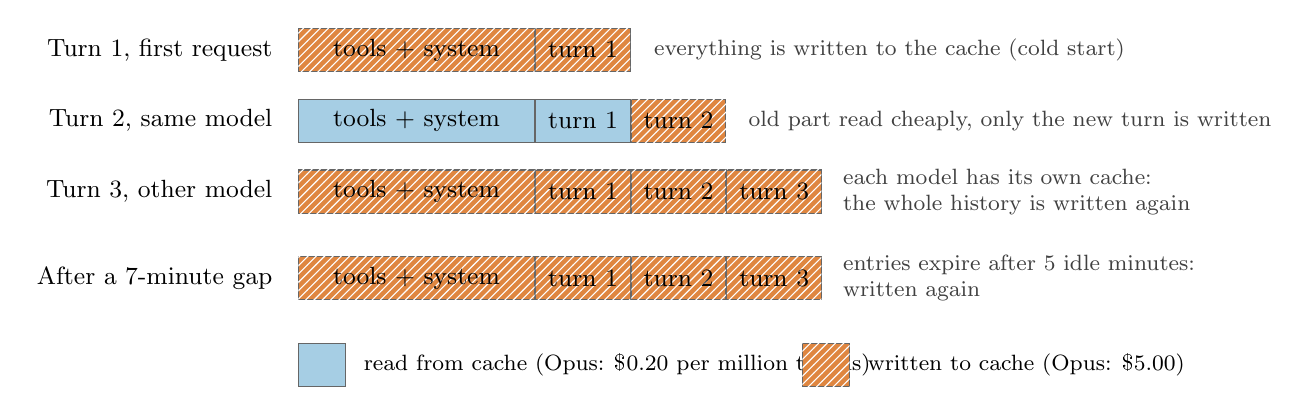
\begin{tikzpicture}[x=1cm, y=1cm, font=\small,
  seg/.style={draw=black!60, minimum height=0.55cm, inner sep=0pt},
  wr/.style={seg, fill=okorange!75, postaction={pattern=north east lines, pattern color=white}},
  rd/.style={seg, fill=okblue!35},
  lab/.style={anchor=east, align=right, font=\small},
  note/.style={anchor=west, align=left, font=\footnotesize, text=black!75}]
  % row 1: first request
  \node[lab] at (0,0) {Turn 1, first request};
  \node[wr, minimum width=3.0cm, anchor=west] (a1) at (0.2,0) {tools + system};
  \node[wr, minimum width=1.2cm, anchor=west] at (a1.east) {turn 1};
  \node[note] at (4.6,0) {everything is written to the cache (cold start)};
  % row 2: same model, next turn
  \node[lab] at (0,-0.9) {Turn 2, same model};
  \node[rd, minimum width=3.0cm, anchor=west] (b1) at (0.2,-0.9) {tools + system};
  \node[rd, minimum width=1.2cm, anchor=west] (b2) at (b1.east) {turn 1};
  \node[wr, minimum width=1.2cm, anchor=west] at (b2.east) {turn 2};
  \node[note] at (5.8,-0.9) {old part read cheaply, only the new turn is written};
  % row 3: switch model
  \node[lab] at (0,-1.8) {Turn 3, other model};
  \node[wr, minimum width=3.0cm, anchor=west] (c1) at (0.2,-1.8) {tools + system};
  \node[wr, minimum width=1.2cm, anchor=west] (c2) at (c1.east) {turn 1};
  \node[wr, minimum width=1.2cm, anchor=west] (c3) at (c2.east) {turn 2};
  \node[wr, minimum width=1.2cm, anchor=west] at (c3.east) {turn 3};
  \node[note] at (7.0,-1.8) {each model has its own cache:\\ the whole history is written again};
  % row 4: long gap
  \node[lab] at (0,-2.9) {After a \LongGapMin-minute gap};
  \node[wr, minimum width=3.0cm, anchor=west] (d1) at (0.2,-2.9) {tools + system};
  \node[wr, minimum width=1.2cm, anchor=west] (d2) at (d1.east) {turn 1};
  \node[wr, minimum width=1.2cm, anchor=west] (d3) at (d2.east) {turn 2};
  \node[wr, minimum width=1.2cm, anchor=west] at (d3.east) {turn 3};
  \node[note] at (7.0,-2.9) {entries expire after \CacheTTLMin\ idle minutes:\\ written again};
  % key
  \node[rd, minimum width=0.6cm, anchor=west] (k1) at (0.2,-4.0) {};
  \node[anchor=west, font=\footnotesize] at (k1.east) {\ read from cache (Opus: \$\PriceOpusRead\ per million tokens)};
  \node[wr, minimum width=0.6cm, anchor=west] (k2) at (6.6,-4.0) {};
  \node[anchor=west, font=\footnotesize] at (k2.east) {\ written to cache (Opus: \$\PriceOpusWrite)};
\end{tikzpicture}

\caption{How the prompt cache behaves over a conversation (schematic, not to scale).}
\label{fig:cache}
\howtoread{Each bar is one request; it always re-sends everything before it. Blue parts are read back from
the cache at the cheap rate; hatched orange parts are written at the expensive rate. Within one model only
the new turn is written. A switch to another model, or a pause longer than the cache's lifetime, makes the
whole history expensive again.}
\end{figure}

\paragraph{What a probe of the provider showed.} Before designing the campaign we sent \ProbeRequests\
deliberately constructed requests straight to the provider (cost \$\ProbeUSD) to pin down the rules that
the design depends on. \Cref{tab:probe} shows the evidence; each row quotes the tokens written and read by
one request.

\begin{table}[htbp]
\centering\small
\caption{The cache-semantics probe. ``P'' is a prompt prefix of \ProbePTokens\ tokens; ``P+X'' a longer
prompt of about \ProbeFullTokens\ tokens; ``Y'' a further \ProbeYTokens-token extension.}
\label{tab:probe}
\begin{tabular*}{\textwidth}{@{\extracolsep{\fill}}>{\raggedright\arraybackslash}p{0.3\textwidth} >{\raggedright\arraybackslash}p{0.38\textwidth} r r@{}}
\toprule
Question & What was sent & tokens written & tokens read \\
\midrule
Longer entry does not serve its own prefix & Write prompt P+X, then ask for P alone & 10{,}948 & 0 \\
 & Ask for P alone again & 0 & 10{,}948 \\
A growing conversation reuses the earlier entry & Write P+X, then send P+X+Y & 2{,}272 & 15{,}455 \\
Two API keys do not share & Write with key 1, same request with key 2 & 15{,}455 & 0 \\
Simultaneous identical requests both pay & Two at the same instant (each) & 15{,}455 & 0 \\
Reads keep an entry alive & Read at 4 min, then again at 7 min & 0 & 15{,}455 \\
 & Never read, asked again at 7 min & 15{,}455 & 0 \\
Each model has its own cache & Written on Sonnet, then sent to Opus & 15{,}454 & 0 \\
Sonnet caches per effort level & Effort medium written, then no effort & 15{,}464 & 0 \\
 & Same pair on Opus & 0 & 15{,}464 \\
\bottomrule
\end{tabular*}

\end{table}

\begin{keyidea}
Six facts from the probe shaped the experiment:
\begin{enumerate}[leftmargin=1.4em]
  \item \textbf{A cache entry exists only where a request marked one, for exactly that prefix.} So one unique
    string at the very start of a session's system prompt (a \term{nonce}) makes every cache entry of that
    session private to it.
  \item \textbf{Each model has its own cache}, and on Sonnet each effort level has its own. A switch starts
    cold, whatever the timing: that cold start \emph{is} the switching cost we want to measure.
  \item \textbf{Two API keys do not share a cache}, but there were not enough keys for one per arm.
  \item \textbf{Two identical requests sent at the same instant both pay the write.} The nonce avoids this
    too, because no two sessions ever send identical requests.
  \item \textbf{Every read keeps an entry alive.} Staggering the arms in time would not isolate them, because
    a running session keeps its shared prefix warm.
  \item \textbf{Entries expire after \CacheTTLMin\ idle minutes.} Long pauses in a conversation are a
    real cost and must be part of the scenarios.
\end{enumerate}
\end{keyidea}


\part{Measuring savings}\label{part:measuring}
\section{Design of the experiment}\label{sec:design}

\subsection{How the design evolved}\label{sec:evolution}

The first design (v1, \path{docs/design/parallel-measurement-mode-v1.md}) wanted to measure the path not taken
\emph{inside} a live session: at a decision point, fork the session, run the other path on the same state, record
its cost, and throw the result away. It proposed single-call forks for prepared actions, turn forks for routing,
and a deferred launch with a ``tail correction'' to undo cache effects. A pre-flight review rejected three parts
of it, and the second design (v2, \path{docs/design/parallel-measurement-mode.md}) is what ran:
\begin{itemize}
  \item \textbf{Single-call forks are not a savings unit.} The probe showed that when a call is skipped, the cache
    write it would have made simply moves to the next call (\cref{sec:caching}); a one-call fork only re-derives
    the estimate it was meant to check.
  \item \textbf{Turn forks measure the wrong thing.} A fork that switches model in the middle of someone else's
    history measures a switch from a foreign history, not what the policy costs in its own world.
  \item \textbf{Power is counted in scenarios.} Cost ratios vary far more between scenarios than within one, so
    the unit of replication had to be the scenario (\cref{sec:power}).
\end{itemize}
v2 replaced forks with whole paired sessions, isolated by a per-session nonce rather than by timing, and treats
cache state as an outcome to be measured, not a nuisance to be corrected.

\subsection{Paired sessions from one frozen snapshot}

The unit of comparison is a \term{pair}: one session of a routed arm and one session of the plain host
(the \term{anchor}) on the same scenario, repetition and host. Both start from the \emph{same} frozen copy
of the workspace and receive the \emph{same} scripted user messages, so any difference in their bills
comes from the policy, not from the task.

All arms of one scenario, repetition and host form a \term{wave}. A wave's sessions are launched within
seconds of each other, each in its own terminal, so they share the time of day and the provider's load.
The launch order was fixed, not randomised: measured from the first session of its wave, the anchor started
on average \StaggerAnchor\,s later, the A/A copy \StaggerAA\,s, shipped \StaggerShipped\,s (at most
\StaggerShippedMax\,s), sticky \StaggerSticky\,s and Sonnet \StaggerSonnet\,s. A small systematic effect of
launch order cannot be ruled out (\cref{sec:aa}). Each session carries its own
nonce, so no arm can read another arm's cache (\cref{sec:caching}). A per-request audit checked every
session for cache reads it could not have written itself; \AuditFlagged\ sessions were flagged.

\begin{keyidea}
\textbf{Pairing removes most of the noise.} Two scenarios can differ in cost by a factor of ten; two arms on
the same scenario differ far less. By comparing each routed session only with its own anchor, the
analysis looks at the ratio within a pair, and the big differences between scenarios cancel out.
\end{keyidea}

\subsection{Arms and hosts}

\begin{table}[htbp]
\centering\small
\caption{The five arms. Every arm except the Sonnet control runs on both host models.}
\label{tab:arms}
\begin{tabular*}{\textwidth}{@{\extracolsep{\fill}}l >{\raggedright\arraybackslash}p{0.62\textwidth}@{}}
\toprule
Arm & What it is, and what comparing it with the anchor tells us \\
\midrule
anchor & The plain host model, no routing. The baseline every other arm is compared with. \\
aa & A second, identical anchor on a seeded \AAPct\,\% subsample. Its ratio to the anchor should be 1: its
  spread is the run-to-run noise floor. \\
shipped & The fast-decisions bundle as shipped (orch-default): its judge re-chooses the model (Sonnet or the
  host) at the start of each turn; it never switched in the middle of a turn (\ShippedMidturn\ mid-turn
  switches in \NShippedSessions\ sessions). \\
sticky & Uses the same routing judge, but only once, on the first prompt; the session then stays on the
  chosen model and never switches. Shipped versus sticky isolates the cost of switching. \\
sonnet & Plain Sonnet for the whole session (``just use the cheap model''). It does not depend on the host,
  so one run serves as the control for both hosts. \\
\bottomrule
\end{tabular*}
\end{table}

The two hosts are Fable 5.1, an expensive model (\cref{tab:prices}), and Opus 5.5, a cheaper one with very
cheap cache reads. The sticky judge chose Sonnet for
\NStickySonnetOnly\ of \NStickySessions\ sticky sessions (\StickyCheap\ of \StickyDecisions\ per host,
\StickyCheapPct\,\%) and the host for the rest, so in practice the sticky arm is mostly ``Sonnet for the whole
session''. The judge's own calls are not part of any session's cost: the sticky decision was made once by the
harness, and the shipped arm's per-turn decisions went to a separate judge service (Jev). Both used the bundle's
default judge, Jev; the post-hoc Cloudflare Clef judges of \cref{sec:clef} were never run in the campaign. An earlier benchmark
measured Jev at \$\JevPerMillion\ per million decisions on comparable real states; at one decision per turn
that adds about \JudgeShippedCents\ cents to a shipped session, \JudgeShippedShare\,\% of a plain Fable
session's cost. That estimate comes from another study and is not measured here.

\subsection{Scenarios}

There are \NScenarios\ scenarios in \NFamilies\ families: \FamPolyglot\ coding exercises from a
multi-language benchmark (polyglot), \FamRepos\ bug fixes and features in small public repositories
(repos), \FamMixed\ mixed coding-and-analysis tasks (mixed), and \FamKnowledge\ documentation, explanation
and review tasks (knowledge). Each is a fixed script of \MinTurns\ to \MaxTurns\ user turns (\MeanTurns\ on
average), identical for every arm, with automatic checks after each turn and hidden tests at the end.
Turns are \ShortGapS\,s apart, except that \NLongGapScen\ scenarios contain \LongGapsPerScen\ pauses of
\LongGapMin\ minutes, longer than the cache's \CacheTTLMin-minute lifetime, so expiry is part of the
workload. The full list is in \cref{tab:scenarios}.

\paragraph{The preregistered split.} Before any session ran, the scenarios were split with a fixed random
seed (\SplitSeed) into \NTrain\ \term{training} scenarios and \NTest\ \term{test} scenarios, balanced by
family and by whether a scenario has long pauses. The savings model is fitted on training scenarios only;
every confirmatory claim uses test scenarios only.

\begin{table}[htbp]
\centering\small
\caption{Scenarios by family and preregistered split.}
\label{tab:families}
\begin{tabular*}{0.7\textwidth}{@{\extracolsep{\fill}}l r r r@{}}
\toprule
Family & training & test & total \\
\midrule
polyglot & \FamPolyglotTrain & \FamPolyglotTest & \FamPolyglot \\
repos & \FamReposTrain & \FamReposTest & \FamRepos \\
mixed & \FamMixedTrain & \FamMixedTest & \FamMixed \\
knowledge & \FamKnowledgeTrain & \FamKnowledgeTest & \FamKnowledge \\
\midrule
all & \NTrain & \NTest & \NScenarios \\
\bottomrule
\end{tabular*}
\end{table}

\subsection{Quality}

A routed arm that saves money by doing worse work has not saved anything. Each turn's checks give a
pass or fail; the \term{turn-pass fraction} is the share of a session's turns that passed. The hidden tests
at the end give a final pass or fail. A savings claim is allowed only where quality is
\term{non-inferior}: the 95\,\% lower bound of the mean difference in turn-pass fraction (arm minus anchor)
must be above \NIMargin, that is, at most \NIMarginPts\ percentage points worse.

\subsection{What a session costs}

Every request's tokens were priced with the fixed table in \cref{tab:prices}; the recomputed cost matched
the provider's reported cost on every session (\CostMismatch\ mismatches). One adjustment makes the
comparison fair. Every session's first request writes the shared tool definitions (about \ToolsAllowance\
tokens) to a cold cache, because the nonce stops sessions from sharing. In production those tools would
usually be warm. The primary \term{tools-normalized} cost re-prices that shared prefix as a cache read; it
changes the campaign total by \$\ToolsDeltaTotal, and every result is also reported on the raw basis
(\cref{sec:rawbasis}).

\subsection{Hypotheses and the decision rule}

The hypotheses, their thresholds, the train/test split and the decision rule were fixed in the
preregistration. Each is tested on the test split only:
\begin{itemize}
  \item \textbf{H1 (Fable host):} sticky and shipped cost less than the anchor (upper end of the interval
    below 1).
  \item \textbf{H2 (Opus host):} routing to Sonnet does not save: sticky, shipped and Sonnet all have a
    lower end above \HTwoLower.
  \item \textbf{H3 (both hosts):} sticky costs no more than shipped (upper end of sticky/shipped at most
    \HThreeUpper).
  \item \textbf{Quality:} every savings claim has non-inferior turn-pass fraction.
\end{itemize}
The decision rule: on a host where H1 holds with non-inferior quality, route (preferring sticky if H3
holds); on a host where H2 holds, do not route to Sonnet. A savings model fitted on training data must
also pass a check on the test data: its 90\,\% prediction intervals must cover between \CovLow\ and
\CovHigh\ of test pairs, and the measured test total must fall inside its predicted interval.

\paragraph{What was fixed later.} The \emph{estimator} was not in the preregistration. The confirmatory
script, \path{evals/paired_confirm.py} (commit \code{\ConfirmSha}), was written after the data were
collected, about \ConfirmAfterMin\ minutes after the campaign finished, when exploratory summaries over all
scenarios (the savings-model output in \path{model/}) already existed. It fixed the number of bootstrap
resamples (\Boot) and the seed (\BootSeed), the pair-level quality filter, which cells count as savings
claims, and the verdict rule, including what ``contradicted'' means. These choices are listed with the other
clarifications in \cref{sec:deviations}; the verdicts under the alternative readings are reported alongside.

\paragraph{Ratios and intervals.} The cost of a pair is summarized as a \term{ratio}, arm cost divided by
anchor cost: 0.80 means 20\,\% cheaper. Ratios are averaged as a \term{geometric mean}, which treats
``twice as expensive'' and ``half as expensive'' symmetrically. A \term{95\,\% confidence interval} gives
the range of ratios consistent with the data. It is computed with a \term{scenario-cluster bootstrap}:
resample whole scenarios (then repetitions) with replacement thousands of times, recompute the ratio each
time, and take the middle 95\,\%. Resampling scenarios rather than single sessions keeps the interval
honest about how much the conclusions depend on which tasks were chosen.

\subsection{How big the experiment had to be}\label{sec:power}

Earlier data gave the spread of log cost ratios between scenarios and within a scenario. Because the
between-scenario spread dominates, precision is bought with more \emph{scenarios}, not more repetitions.
\Cref{tab:power} shows the half-widths the design document projected; the campaign used \NScenarios\
scenarios and \NReps\ repetitions.

\begin{table}[htbp]
\centering\small
\caption{Projected precision of the routing ratio, from the design document (before the campaign). The
projections assumed \PowerSA\ and \PowerSB\ scenarios; the confirmatory test split has \NTest, so its
intervals are wider than these.}
\label{tab:power}
\begin{tabular*}{\textwidth}{@{\extracolsep{\fill}}l r r r r@{}}
\toprule
 & \multicolumn{2}{c}{SD of log ratio} & \multicolumn{2}{c}{95\,\% CI half-width} \\
\cmidrule(lr){2-3}\cmidrule(l){4-5}
Contrast (earlier data) & between scenarios & within & \PowerSA\ scenarios & \PowerSB\ scenarios \\
\midrule
Routing, Fable (s1m values) & 0.265 & 0.297 & $\pm$9\,\% & $\pm$11\,\% \\
Routing, Fable (S1 values, worst case) & 0.433 & 0.258 & $\pm$13\,\% & $\pm$16\,\% \\
Routing, Opus (S1 values) & 0.162 & 0.266 & $\pm$7\,\% & $\pm$8\,\% \\
Routing, Opus (s1m values) & 0.027 & 0.211 & $\pm$4\,\% & $\pm$5\,\% \\
\bottomrule
\end{tabular*}

\end{table}

Behind that table is a variance analysis of \PowerPairs\ earlier pairs (\path{step0_variance.json}). For the
shipped router on the Fable host in \CaTurns-turn sessions, the between-scenario standard deviation of the log
ratio was \PowFableFourSB\ against \PowFableFourSW\ within a scenario; on Opus it was \PowOpusFourSB\ against
\PowOpusFourSW. \Cref{fig:power} turns these into the interval one should expect for a given number of scenarios.

\begin{figure}[htbp]
\centering
\pgfplotslegendfromname{powerlegend}\par\smallskip
% Projected 95% CI half-width of the cost ratio vs number of scenarios (2 repetitions), from step0_variance.json.
\begin{tikzpicture}
\begin{axis}[benchmark, scale only axis, width=11cm, height=5.2cm, xmin=10, xmax=100, ymin=0, ymax=40,
  xlabel={Number of scenarios (2 repetitions each)}, ylabel={95\,\% CI half-width (\%)}, xmajorgrids, ymajorgrids,
  title={Precision is bought with scenarios}, title style={font=\small\bfseries},
  cycle list={{okblue, mark=*, solid}, {okblue, mark=o, dashed}, {okorange, mark=square*, solid}, {okorange, mark=square, dashed}},
  every axis plot/.append style={line width=1pt, mark size=1.8pt, mark repeat=2},
  legend to name=powerlegend, legend columns=4, legend cell align=left,
  legend style={/tikz/every even column/.append style={column sep=8pt}}]
\addplot+ table[x=S, y=c0]{generated/data/power-curve.dat};
\addplot+ table[x=S, y=c1]{generated/data/power-curve.dat};
\addplot+ table[x=S, y=c2]{generated/data/power-curve.dat};
\addplot+ table[x=S, y=c3]{generated/data/power-curve.dat};
\addlegendentry{Fable, 1-turn}
\addlegendentry{Fable, 4-turn}
\addlegendentry{Opus, 1-turn}
\addlegendentry{Opus, 4-turn}

\draw[okgray, densely dashed, line width=0.8pt] (axis cs:\NTest,0) -- (axis cs:\NTest,40);
\draw[okgray, densely dashed, line width=0.8pt] (axis cs:\NScenarios,0) -- (axis cs:\NScenarios,40);
\node[font=\scriptsize, anchor=south west, fill=white, inner sep=1pt] at (axis cs:\NTest,34) {test split};
\node[font=\scriptsize, anchor=south west, fill=white, inner sep=1pt] at (axis cs:\NScenarios,34) {all scenarios};
\end{axis}
\end{tikzpicture}

\caption{Projected 95\,\% interval half-width of the cost ratio against the number of scenarios (two repetitions
each), from the earlier data's between- and within-scenario variance.}
\label{fig:power}
\howtoread{Lower is more precise. Each line is one earlier configuration (host, session length). The curves fall
quickly at first and then flatten: going from \NTest\ to \NScenarios\ scenarios roughly halves the uncertainty.
The Fable single-turn line is high because those ratios varied a lot between tasks.}
\end{figure}

\subsection{The pilot}

Two small screening pilots preceded the preregistration; the second ran \PilotSessions\ sessions on
\PilotScen\ scenarios. They confirmed the plumbing (nonce isolation, cache audit, quality checks) and
measured the A/A noise: a standard deviation of the log ratio of \PilotSDFable\ on Fable and \PilotSDOpus\
on Opus. Their cost ratios became the hypotheses above, not findings; they are compared with the final
numbers in \cref{sec:interim}.

\begin{figure}[htbp]
\centering
\pgfplotslegendfromname{pilotlegend}\par\smallskip
% Pilot-2 cost ratios against the final all-split ratios (95% CI) per arm and host.
\begin{tikzpicture}
\begin{axis}[benchmark, scale only axis, width=10.5cm, height=5cm, xmode=log, log ticks with fixed point,
  xtick={0.5,0.6,0.8,1,1.2,1.4,1.6}, xmin=0.45, xmax=1.8, ymin=-0.6, ymax=8.6, ytick={0,1,2,3,5,6,7,8},
  yticklabels from table={generated/data/pilot.dat}{label}, xmajorgrids,
  title={Pilot screen versus the full campaign}, title style={font=\small\bfseries},
  xlabel={Cost ratio against the plain host (log scale)},
  legend to name=pilotlegend, legend columns=2, legend cell align=left,
  legend style={/tikz/every even column/.append style={column sep=10pt}}]
\draw[black!70, line width=0.8pt] (axis cs:1,-0.6) -- (axis cs:1,8.6);
\addplot[only marks, mark=*, mark size=2.6pt, color=okblue, error bars/.cd, x dir=both, x explicit,
  error bar style={line width=1pt}] table[x=final, y=y, x error minus=fm, x error plus=fp]{generated/data/pilot.dat};
\addlegendentry{full campaign, all scenarios (95\,\% CI)}
\addplot[only marks, mark=diamond*, mark size=3.2pt, color=okorange] table[x=pilot, y expr=\thisrow{y}-0.3]{generated/data/pilot.dat};
\addlegendentry{pilot-2 (\PilotScenariosN\ scenarios)}
\end{axis}
\end{tikzpicture}

\caption{The second screening pilot (\PilotPairs\ pairs on \PilotScenariosN\ scenarios) against the full campaign
(all scenarios, 95\,\% intervals), for each arm and host. The first pilot was a smoke test of the harness
(\$\SpendPilotOne) whose rows were not packaged.}
\label{fig:pilot}
\howtoread{Diamonds are the pilot, dots and whiskers the final result. On Fable the diamonds sit inside or near
the whiskers; on Opus the pilot overstated the extra cost. A five-scenario pilot was good for finding the
direction, not the size.}
\end{figure}

\section{Running it safely}\label{sec:running}

\subsection{The memory guard}

On the day the campaign was prepared, a validation run nearly ended it. An unguarded Go test binary from
one scenario grew to between \MemGrowLow\ and \MemGrowHigh\,GB of memory and drove the
\MemMacGB\,GB workstation out of memory \MemTimes\ times, taking the terminal server down with it. A
benchmark that occasionally crashes its own machine produces gaps that are not random: the heavy scenarios
go missing.

The operating system's own out-of-memory killer (JetsamEvents in the macOS logs) recorded each of those events. From then on nothing that executes scenario code ran unguarded:
\begin{itemize}
  \item \textbf{memguard} runs every grader and hidden test in its own process group, measures the memory
    of the whole process tree every \MemPollS\,s, and kills it above \MemGraderGB\,GB or after
    \MemGraderS\,s. Such a kill counts as a failed check, never as a crash.
  \item \textbf{A watchdog} in the campaign runner checks every \MemWatchS\,s. It kills an agent session
    above \KillCap\,GB, pauses new waves when free memory runs low, and below \MemHardFloorGB\,GB kills the
    newest sessions first.
  \item \textbf{The same limits apply to every arm}, so the guard cannot favour one policy.
\end{itemize}

\begin{keyidea}
A guard that kills runaway sessions is only fair if its kills are counted, not hidden. The one session the
watchdog killed (\KillSession: \KillRSS\,GB against an \KillCap\,GB cap) was kept as a quality outcome
(turn-pass fraction \KillTurnPass) and excluded only from cost comparisons, which is why
\NPairsValid\ of the \NPairs\ pairs are cost-valid.
\end{keyidea}

\subsection{Failures and retries}

A \term{wave attempt} that failed for an infrastructure reason was rerun as a whole, so that all arms of a
wave always shared the same conditions. Of \NAttempts\ wave attempts, \NWaves\ were accepted, one per wave,
and \NFailed\ failed. Every failed attempt was an infrastructure failure, every wave eventually completed,
and no wave is missing from the data. \NWavesReset\ waves were excluded after three failures and then reset
and rerun by hand.

\begin{table}[htbp]
\centering\small
\caption{Failed wave attempts by cause. For \NFailedInferred\ of them the cause was not recorded at the time
and is inferred from timing.}
\label{tab:failures}
\begin{tabular*}{\textwidth}{@{\extracolsep{\fill}}l r r r@{}}
\toprule
Cause & failed attempts & sessions in them & spend \\
\midrule
Terminal-server session cap (harness bug) & 31 & 119 & \$0.00 \\
Terminal-server daemon restart & 11 & 37 & \$48.51 \\
Laptop lid closed on battery & 7 & 20 & \$55.46 \\
\midrule
Total & 49 & 176 & \$103.97 \\
\bottomrule
\end{tabular*}

\end{table}

The largest group was a harness bug: after a restart at high parallelism, the runner launched more
terminals than the terminal server allowed, and the excess launches failed at once without spending
anything. The fix (wait for capacity) went into the running harness that evening. Restarts of the terminal
server killed sessions mid-run; a circuit breaker then paused and resumed the campaign. The laptop's lid
being closed on battery put the machine to sleep twice, and those attempts timed out.

\subsection{What the live dashboard showed}

During the run a local dashboard refreshed every minute with progress, throughput and spend. Its final snapshot
is packaged as \path{dashboard/index.html}. \Cref{fig:progress} rebuilds the same views from the session rows and
the failure log, so it can be checked against the data.

\begin{figure}[htbp]
\centering
\pgfplotslegendfromname{progresslegend}\par\smallskip
% Campaign progress reconstructed from session rows and FAILURES.md: completed sessions, spend, hourly throughput.
\begin{tikzpicture}
\begin{groupplot}[benchmark, group style={group size=1 by 3, vertical sep=0.9cm, xlabels at=edge bottom, xticklabels at=edge bottom},
  scale only axis, width=12cm, height=2.6cm, xmin=0, xmax=\ProgressMaxH, xmajorgrids, ymajorgrids,
  title style={font=\small\bfseries}]
\nextgroupplot[title={Sessions completed}, ylabel={sessions}, ymin=0,
  legend to name=progresslegend, legend columns=4, legend cell align=left,
  legend style={/tikz/every even column/.append style={column sep=8pt}}]
\addplot[okblue, line width=1pt] table[x=h, y=sessions]{generated/data/progress.dat};
\addlegendentry{accepted sessions}
\addplot[only marks, mark=x, mark size=3pt, color=okorange, line width=1pt] table[x=h, y expr=40, restrict expr to domain={\thisrow{cause}}{0:0}]{generated/data/failures-time.dat};
\addlegendentry{failed: session cap}
\addplot[only marks, mark=triangle*, mark size=3pt, color=black] table[x=h, y expr=120, restrict expr to domain={\thisrow{cause}}{1:1}]{generated/data/failures-time.dat};
\addlegendentry{failed: daemon restart}
\addplot[only marks, mark=o, mark size=3pt, color=okgreen, line width=1pt] table[x=h, y expr=200, restrict expr to domain={\thisrow{cause}}{2:2}]{generated/data/failures-time.dat};
\addlegendentry{failed: laptop asleep}
\nextgroupplot[title={Spend on accepted sessions}, ylabel={US dollars}, ymin=0]
\addplot[okorange, line width=1pt] table[x=h, y=spend]{generated/data/progress.dat};
\nextgroupplot[title={Sessions completed per hour}, ylabel={sessions}, xlabel={Hours since the first session}, ymin=0,
  ybar, bar width=3pt]
\addplot[fill=okgreen!70, draw=black!60] table[x=h, y=n]{generated/data/throughput.dat};
\end{groupplot}
\end{tikzpicture}

\caption{Campaign progress reconstructed from the data: accepted sessions completed and their spend over the
\ProgressHours\ hours from the first session to the last, sessions completed per hour, and when failed attempts
started, by cause.}
\label{fig:progress}
\howtoread{Flat stretches in the top two panels are pauses: the laptop asleep, a terminal-server restart, or the
runner waiting for capacity. The markers on the top panel show when failed attempts started; the burst of crosses
is the session-cap bug, which cost nothing because those launches failed immediately. The bottom panel peaks at
\ThroughputMax\ sessions in an hour.}
\end{figure}

\subsection{Spend and time}

The campaign ledger recorded \$\SpendLedger\ against a hard stop of \$\SpendBudget: \$\SpendSessions\ for
the accepted sessions, \$\NFailedUSD\ for failed attempts and \$\SpendPreflight\ for preflight checks. The
two pilots cost \$\SpendPilots. The first session started at \FirstStart\ UTC and the campaign completed at
\CompleteEDT\ EDT the next day, about \WallHours\ hours.

\paragraph{Provenance.} The preregistration was committed at \PreregTime\ EDT (commit \code{\PreregSha});
the first session started \PreregGapMin\ minutes and \PreregGapSec\ seconds later. The agent under test was
frozen at that same commit in every session. The campaign \emph{harness}, however, ran from uncommitted
working-tree code and was committed afterwards (\code{\HarnessSha}); re-extracting the rows with the
committed harness reproduces them byte for byte (\cref{sec:repro}).

\section{Confirmatory results}\label{sec:confirm}

Everything in this section uses the \NTest\ test scenarios only (\NTestPairs\ pairs). The hypotheses,
thresholds and decision rule are the preregistered ones; the estimator (resamples, seed, quality filter,
verdict rule) was fixed afterwards in the confirmatory script (\cref{sec:design}). The results below depend on
that estimator, so this section is labelled confirmatory but not preregistered. The preregistration said the cost ratio is computed ``among pairs where quality is
non-inferior.'' That sentence has two readings, so both are reported:
\begin{itemize}
  \item \textbf{Pair reading (co-primary):} keep a pair only if its own turn-pass fraction is not worse than
    its anchor's by more than \NIMarginPts\ points. In this design that keeps pairs where the arm did at
    least as well. Because this filter conditions on an outcome the arm affects, it is not reported alone.
  \item \textbf{Arm reading (co-primary, unfiltered):} keep every cost-valid pair, and require non-inferiority of
    the arm as a whole.
\end{itemize}

\begin{table}[htbp]
\centering\small
\caption{Primary endpoint: geometric-mean cost ratio, arm over plain host, test split, with 95\,\%
scenario-cluster bootstrap intervals. ``Pairs kept'' counts pairs that pass the pair-level quality filter
out of all cost-valid test pairs.}
\label{tab:primary}
\begin{tabular*}{\textwidth}{@{\extracolsep{\fill}}l l r r r r r@{}}
\toprule
 & & \multicolumn{3}{c}{Pair reading (co-primary)} & \multicolumn{2}{c}{Arm reading (co-primary, unfiltered)} \\
\cmidrule(lr){3-5}\cmidrule(l){6-7}
Host & Arm & pairs kept & ratio & 95\,\% CI & ratio & 95\,\% CI \\
\midrule
Fable 5.1 & sticky & \CfFableStickyPairN/\CfFableStickyNValid & \CfFableStickyPair & \CfFableStickyPairCI & \CfFableStickyArm & \CfFableStickyArmCI \\
Fable 5.1 & shipped & \CfFableShippedPairN/\CfFableShippedNValid & \CfFableShippedPair & \CfFableShippedPairCI & \CfFableShippedArm & \CfFableShippedArmCI \\
Fable 5.1 & sonnet & \CfFableSonnetPairN/\CfFableSonnetNValid & \CfFableSonnetPair & \CfFableSonnetPairCI & \CfFableSonnetArm & \CfFableSonnetArmCI \\
\addlinespace[3pt]
Opus 5.5 & sticky & \CfOpusStickyPairN/\CfOpusStickyNValid & \CfOpusStickyPair & \CfOpusStickyPairCI & \CfOpusStickyArm & \CfOpusStickyArmCI \\
Opus 5.5 & shipped & \CfOpusShippedPairN/\CfOpusShippedNValid & \CfOpusShippedPair & \CfOpusShippedPairCI & \CfOpusShippedArm & \CfOpusShippedArmCI \\
Opus 5.5 & sonnet & \CfOpusSonnetPairN/\CfOpusSonnetNValid & \CfOpusSonnetPair & \CfOpusSonnetPairCI & \CfOpusSonnetArm & \CfOpusSonnetArmCI \\
\bottomrule
\end{tabular*}

\end{table}
\howtoreadtable{A ratio below 1 is a saving: \CfFableStickyPair\ means the routed arm paid about
\CfFableStickyCents\ cents for every dollar the plain host paid. If the whole interval is below 1, the
cost difference is not explained by chance; if it is above 1, neither is the extra cost. The pair-level filter drops sessions
that were cheaper but did worse, so for sticky and shipped it raises the ratio by \FilterLiftLow\ to
\FilterLiftHigh; on Opus the arm reading gives \CfOpusStickyArmExtra--\CfOpusSonnetArmExtra\,\% more
than the plain host.}

\begin{figure}[htbp]
\centering
\pgfplotslegendfromname{forestlegend}\par\smallskip
% Confirmatory cost ratios (test split) with 95% scenario-cluster bootstrap CIs. Log x axis.
\begin{tikzpicture}
\begin{axis}[benchmark, xmode=log, log ticks with fixed point,
  xtick={0.5,0.6,0.7,0.8,0.9,1,1.2,1.4,1.6}, xmin=0.45, xmax=1.75,
  scale only axis, width=10.5cm, xmajorgrids, y tick label style={font=\small}, height=5.2cm, ymin=-0.7, ymax=6.7,
  ytick={0,1,2,4,5,6}, yticklabels from table={generated/data/forest.dat}{label},
  xlabel={Cost ratio, routed arm / plain host (log scale; below 1 saves money)},
  legend to name=forestlegend, legend columns=2, legend cell align=left,
  legend style={/tikz/every even column/.append style={column sep=10pt}}]
\draw[black!70, line width=0.8pt] (axis cs:1,-0.7) -- (axis cs:1,6.7);
\draw[okgray, dashed, line width=0.8pt] (axis cs:\HTwoLower,-0.7) -- (axis cs:\HTwoLower,2.6);
\addplot[only marks, mark=*, mark size=2.6pt, color=okblue,
  error bars/.cd, x dir=both, x explicit, error bar style={line width=1pt}]
  table[x=pair, y=y, x error minus=pm, x error plus=pp]{generated/data/forest.dat};
\addlegendentry{pair reading (co-primary)}
\addplot[only marks, mark=diamond, mark size=3pt, color=okorange, mark options={line width=1pt},
  error bars/.cd, x dir=both, x explicit, error bar style={line width=0.6pt, densely dashed}]
  table[x=arm, y expr=\thisrow{y}-0.3, x error minus=am, x error plus=ap]{generated/data/forest.dat};
\addlegendentry{arm reading (co-primary, unfiltered)}
\end{axis}
\end{tikzpicture}

\smallskip
\begin{tikzpicture}
\begin{axis}[benchmark, xmode=log, log ticks with fixed point,
  xtick={0.5,0.6,0.7,0.8,0.9,1,1.2,1.4,1.6}, xmin=0.45, xmax=1.75,
  scale only axis, width=10.5cm, xmajorgrids, y tick label style={font=\small}, height=1.6cm, ymin=-0.7, ymax=1.7,
  ytick={0,1}, yticklabels from table={generated/data/forest-h3.dat}{label},
  xlabel={Cost ratio, sticky / shipped on the same scenario (H3; log scale)}]
\draw[black!70, line width=0.8pt] (axis cs:1,-0.7) -- (axis cs:1,1.7);
\draw[okgray, dashed, line width=0.8pt] (axis cs:\HThreeUpper,-0.7) -- (axis cs:\HThreeUpper,1.7);
\addplot[only marks, mark=*, mark size=2.6pt, color=okblue,
  error bars/.cd, x dir=both, x explicit, error bar style={line width=1pt}]
  table[x=pair, y=y, x error minus=pm, x error plus=pp]{generated/data/forest-h3.dat};
\addplot[only marks, mark=diamond, mark size=3pt, color=okorange, mark options={line width=1pt},
  error bars/.cd, x dir=both, x explicit, error bar style={line width=0.6pt, densely dashed}]
  table[x=arm, y expr=\thisrow{y}-0.3, x error minus=am, x error plus=ap]{generated/data/forest-h3.dat};
\end{axis}
\end{tikzpicture}

\caption{Confirmatory cost ratios on the test split. Top: each routed arm against the plain host. Bottom: the
sticky arm against the shipped arm on the same scenarios (H3). Whiskers are 95\,\% intervals. The solid line
marks 1 (no difference); the dashed lines mark the preregistered thresholds for H2 (\HTwoLower) and H3
(\HThreeUpper).}
\label{fig:forest}
\howtoread{Each row is one comparison; the dot is the best estimate and the whisker the 95\,\% interval.
The horizontal axis is logarithmic, so ``half the cost'' and ``double the cost'' are the same distance from
1. All three Fable rows lie well left of 1 (savings); all three Opus rows lie right of the dashed line
(no saving). In the bottom panel both hosts lie left of 1: the sticky policy cost less than the shipped one, by a
small margin on Fable.}
\end{figure}

\subsection{The hypotheses}

\begin{table}[htbp]
\centering\small
\caption{The preregistered hypotheses, test split, pair reading. The arm reading gives the same verdicts.}
\label{tab:hyp}
\begin{tabular*}{\textwidth}{@{\extracolsep{\fill}}>{\raggedright\arraybackslash}p{0.33\textwidth} l l r r l@{}}
\toprule
Hypothesis (test split, pair reading) & Host & Arm & ratio & 95\,\% CI & verdict \\
\midrule
H1: routing is cheaper (upper end $<$ 1) & Fable & sticky & \CfFableStickyPair & \CfFableStickyPairCI & \vconf \\
H1: routing is cheaper (upper end $<$ 1) & Fable & shipped & \CfFableShippedPair & \CfFableShippedPairCI & \vconf \\
H2: no saving (lower end $>$ \HTwoLower) & Opus & sticky & \CfOpusStickyPair & \CfOpusStickyPairCI & \vconf \\
 & Opus & shipped & \CfOpusShippedPair & \CfOpusShippedPairCI & \vconf \\
 & Opus & sonnet & \CfOpusSonnetPair & \CfOpusSonnetPairCI & \vconf \\
H3: sticky/shipped (upper end $\le$ \HThreeUpper) & Fable & sticky/shipped & \HThreeFable & \HThreeFableCI & \vconf \\
 & Opus & sticky/shipped & \HThreeOpus & \HThreeOpusCI & \vconf \\
\bottomrule
\end{tabular*}

\end{table}

\begin{itemize}
  \item \textbf{H1, confirmed.} On the Fable host, sticky cost \CfFableStickyPair\X\ (95\,\% CI
    \CfFableStickyPairCI) and shipped \CfFableShippedPair\X\ (\CfFableShippedPairCI) of the plain host.
  \item \textbf{H2, confirmed.} On the Opus host, sticky cost \CfOpusStickyPair\X\ (\CfOpusStickyPairCI),
    shipped \CfOpusShippedPair\X\ (\CfOpusShippedPairCI) and plain Sonnet \CfOpusSonnetPair\X\
    (\CfOpusSonnetPairCI): routing to Sonnet costs about \CfOpusStickyExtra--\CfOpusSonnetExtra\,\% more.
  \item \textbf{H3, confirmed.} The preregistered test was only that sticky costs no more than shipped
    (upper end at most \HThreeUpper). Sticky cost \HThreeFable\X\ of shipped on Fable (\HThreeFableCI) and
    \HThreeOpus\X\ on Opus (\HThreeOpusCI), on \HThreeFableN\ and \HThreeOpusN\ matched scenario
    repetitions. On Fable the upper end, \HThreeFableUpper, is close to 1.
\end{itemize}

\subsection{Quality}

\begin{table}[htbp]
\centering\small
\caption{Quality: mean difference in turn-pass fraction, arm minus plain host, test split, all quality-valid
pairs. Non-inferior when the lower end of the interval is above \NIMargin.}
\label{tab:quality}
\begin{tabular*}{\textwidth}{@{\extracolsep{\fill}}l l r r r l@{}}
\toprule
Host & Arm & pairs & mean $\Delta$ turn-pass & 95\,\% CI & non-inferior \\
\midrule
Fable 5.1 & sticky & 46 & \QFableSticky & \QFableStickyCI & \vconf \\
Fable 5.1 & shipped & 46 & \QFableShipped & \QFableShippedCI & \vconf \\
Fable 5.1 & sonnet & 46 & \QFableSonnet & \QFableSonnetCI & \vconf \\
Opus 5.5 & sticky & 46 & \QOpusSticky & \QOpusStickyCI & \textcolor{okorange}{\textsf{not confirmed}} \\
Opus 5.5 & shipped & 46 & \QOpusShipped & \QOpusShippedCI & \vconf \\
Opus 5.5 & sonnet & 46 & \QOpusSonnet & \QOpusSonnetCI & \vconf \\
\bottomrule
\end{tabular*}

\end{table}

Every Fable savings claim passes the quality test. (A \term{savings claim} here is any arm and host whose
own cost interval shows a saving; only those cells are tested for quality.) The closest call is Fable sticky,
whose lower bound is \QFableStickyLow, inside the \NIMargin\ margin by only \QFableStickyMarginGap.
Across all \QAllScen\ scenarios (exploratory) its mean difference is \QAllFableSticky\ with a 95\,\%
interval of \QAllFableStickyCI: there the margin is not shown, and on the \NTrain\ training scenarios it is
\RvQTrainFableSticky\ (\RvQTrainFableStickyCI). So quality passed on the test split only. The quality test itself
is unfiltered: it uses every quality-valid test pair, so the \QFableStickyMarginGap\ margin does not depend on the
pair-level cost filter. That margin is close to the Monte-Carlo noise of the bootstrap: re-drawing the resamples
with a different random stream moves the lower bound by \RvQNoise\ (to \RvQAltLow). Opus sticky did not show
non-inferior quality (\QOpusSticky, 95\,\% CI \QOpusStickyCI; ``not shown'', which is not the same as ``worse'').
The preregistration requires quality for each savings claim, and no savings claim is made on Opus, so the quality
hypothesis is confirmed under that scope; if quality were required of every routed cell, \RvNQualCells\ of
\RvNRoutedCells\ cells would pass and \RvNHypAllQuality\ of 4 hypotheses would be confirmed.

\subsection{The savings model}\label{sec:modelcheck}

The preregistered deliverable is a model that predicts the saving of a new session from what is known before
it starts: arm, host, task type, number of turns, long pauses and the size of the first prompt. It was fitted
on the training scenarios only and then asked to predict the \MCPairs\ held-out test pairs.

\begin{figure}[htbp]
\centering
\pgfplotslegendfromname{modellegend}\par\smallskip
% Prediction model check on the test split: predicted total saving (with 90% PI) vs observed, per arm and host.
\begin{tikzpicture}
\begin{axis}[benchmark, scale only axis, width=\ModelAxisW, height=\ModelAxisH,
  xmin=-70, xmax=150, ymin=-70, ymax=150,
  xtick={-50,0,50,100,150}, ytick={-50,0,50,100,150},
  xlabel={Predicted total saving on the test pairs (\$; whisker: 90\,\% interval)},
  ylabel={Observed total saving (\$)}, xmajorgrids, ymajorgrids, clip=false,
  legend to name=modellegend, legend columns=3, legend cell align=left,
  legend style={/tikz/every even column/.append style={column sep=10pt}}]
\addplot[okgray, dashed, line width=0.8pt, domain=-70:150, samples=2] {x};
\addlegendentry{prediction = observation}
\addplot[only marks, mark=*, mark size=2.6pt, color=okblue,
  error bars/.cd, x dir=both, x explicit, error bar style={okblue!60, line width=0.7pt}]
  table[x=pred, y=obs, x error minus=minus, x error plus=plus]{generated/data/model-check-fable.dat};
\addlegendentry{Fable host}
\addplot[only marks, mark=square*, mark size=2.6pt, color=okorange,
  error bars/.cd, x dir=both, x explicit, error bar style={okorange!60, line width=0.7pt}]
  table[x=pred, y=obs, x error minus=minus, x error plus=plus]{generated/data/model-check-opus.dat};
\addlegendentry{Opus host}
% Generated by build_assets.py: labels for panel model-check. Do not edit.
\node[scatterlabel, anchor=north] at ($(axis cs:93.5700,85.0100)+(0.000pt,-4.700pt)$) {shipped, Fable};
\node[scatterlabel, anchor=north west] at ($(axis cs:-32.6400,-31.4800)+(3.323pt,-3.323pt)$) {shipped, Opus};
\node[scatterlabel, anchor=east] at ($(axis cs:69.1800,94.9500)+(-4.700pt,0.000pt)$) {sonnet, Fable};
\node[scatterlabel, anchor=north] at ($(axis cs:-42.5100,-46.8000)+(0.000pt,-4.700pt)$) {sonnet, Opus};
\node[scatterlabel, anchor=west] at ($(axis cs:103.1300,99.8200)+(4.700pt,0.000pt)$) {sticky, Fable};
\node[scatterlabel, anchor=west] at ($(axis cs:-28.6900,-21.1500)+(4.700pt,0.000pt)$) {sticky, Opus};

\end{axis}
\end{tikzpicture}

\caption{The savings model on the test split: predicted total saving (with its 90\,\% interval) against the
observed total, for each arm and host.}
\label{fig:model}
\howtoread{A point on the dashed diagonal is a perfect prediction. Every whisker crosses the diagonal, so
every observed total lies inside its predicted 90\,\% interval. Points above zero are savings (Fable);
points below zero are extra costs (Opus).}
\end{figure}

The model passed both preregistered checks. Its 90\,\% intervals covered \MCCovLog\ of test pairs on the log
ratio and \MCCovUSD\ on the dollar saving, both inside [\CovLow, \CovHigh]. The observed test total,
\$\MCObserved, lay inside the predicted interval of \$\MCPILow\ to \$\MCPIHigh\ (point prediction
\$\MCPredicted). The intervals are conservative: they covered \MCCovLog\ of pairs against a nominal
\MCNominal. The pooled total nets Fable savings (\$\MCFableTotal) against Opus losses (\$\MCOpusTotal), so
it says little about either host on its own. The design document's stricter criteria (coverage
\DesignCovLow--\DesignCovHigh, calibration slope \DesignSlopeLow--\DesignSlopeHigh) are also met (slope
\MCSlope). \Cref{tab:modelcheck} in the appendix gives the check for each arm and host. The verdict is
``\MCVerdict''; its limits are discussed in \cref{sec:modellimits}.

\subsection{Decision}

Applying the preregistered rule: on the Fable host, \textbf{\DecisionFable}; on the Opus host,
\textbf{\DecisionOpus}. Every verdict was re-derived under both non-inferiority readings and under
\NSeeds\ other bootstrap seeds (\SeedLo--\SeedHi); \SeedsChanged\ verdicts changed. The other
clarifications of the preregistration (\cref{sec:deviations}) were not re-run separately.

\section{Exploratory results \texorpdfstring{\screen}{[screen]}}\label{sec:explore}

Everything in this section was not preregistered, or uses all \NScenarios\ scenarios (training and test
together). It explains and qualifies the confirmatory results; it does not confirm anything on its own.

\subsection{Where the cost comes from}\label{sec:composition}

\begin{figure}[htbp]
\centering
\pgfplotslegendfromname{complegend}\par\smallskip
% Where the money goes: mean tools-normalized cost per session, split by token class.
\begin{tikzpicture}
\begin{axis}[benchmark, xbar stacked, bar width=10pt, scale only axis, width=10.5cm, height=6.4cm,
  xmin=0, xmax=\CompMax, ymin=-0.6, ymax=6.6, ytick={0,...,6},
  yticklabels from table={generated/data/composition.dat}{label},
  xlabel={Mean cost per session (US dollars)}, xmajorgrids,
  legend to name=complegend, legend columns=3, legend cell align=left,
  legend style={/tikz/every even column/.append style={column sep=10pt}}]
\addplot[fill=okgray!50, draw=black!60] table[x=input, y=idx]{generated/data/composition.dat};
\addlegendentry{uncached input}
\addplot[fill=okblue!45, draw=black!60] table[x=read, y=idx]{generated/data/composition.dat};
\addlegendentry{cache read}
\addplot[fill=okorange!80, draw=black!60, postaction={pattern=north east lines, pattern color=white}]
  table[x=write, y=idx]{generated/data/composition.dat};
\addlegendentry{cache write (new content)}
\addplot[fill=black!75, draw=black!60, postaction={pattern=crosshatch dots, pattern color=white}]
  table[x=rebuild, y=idx]{generated/data/composition.dat};
\addlegendentry{rebuild after a switch}
\addplot[fill=okgreen!70, draw=black!60, postaction={pattern=dots, pattern color=white}]
  table[x=output, y=idx]{generated/data/composition.dat};
\addlegendentry{output}
\end{axis}
\end{tikzpicture}

\caption{Mean cost per session, split by what was paid for (all splits, cost-valid sessions,
tools-normalized). ``Rebuild after a switch'' is the extra paid for re-writing history to a new model's
cache.}
\label{fig:composition}
\howtoread{Each bar is one kind of session; its length is the average bill and its segments show what the
bill was for. Compare the three Fable bars with each other, and the three Opus bars with each other. On
Fable, routing shrinks the large hatched ``cache write'' segment. On Opus, routing lengthens the blue
``cache read'' segment.}
\end{figure}

\begin{table}[htbp]
\centering\small
\caption{The numbers behind \cref{fig:composition}: dollars per session by token class, main-loop requests per
session, and cache-read tokens per session (millions).}
\label{tab:composition}
\begin{tabular*}{\textwidth}{@{\extracolsep{\fill}}l r r r r r r r r@{}}
\toprule
 & & & \multicolumn{4}{c}{of which (\$ per session)} & & \\
\cmidrule(lr){4-7}
Session kind & sessions & \$/session & cache read & cache write & rebuild & output & requests & tokens read \\
\midrule
Fable: plain host & 140 & 5.31 & 1.06 & 2.82 & 0.00 & 1.27 & 46.0 & 4.22\,M \\
Fable: shipped & 140 & 3.56 & 1.37 & 0.97 & 0.61 & 0.49 & 50.6 & 4.68\,M \\
Fable: sticky & 140 & 3.33 & 1.34 & 1.40 & 0.00 & 0.45 & 50.2 & 4.58\,M \\
Sonnet only (control) & 140 & 3.22 & 1.77 & 0.96 & 0.00 & 0.44 & 57.4 & 5.90\,M \\
Opus: plain host & 140 & 2.13 & 0.62 & 1.04 & 0.00 & 0.40 & 36.4 & 3.07\,M \\
Opus: shipped & 140 & 2.71 & 1.28 & 0.77 & 0.29 & 0.32 & 48.9 & 4.43\,M \\
Opus: sticky & 140 & 2.61 & 1.28 & 0.95 & 0.00 & 0.33 & 48.5 & 4.43\,M \\
\bottomrule
\end{tabular*}

\end{table}

\Cref{fig:composition,tab:composition} show why the two hosts disagree.
\begin{itemize}
  \item \textbf{On Fable, routing cuts the most expensive line.} A plain Fable session paid \$\CompFableAnchorWrite\
    of its \$\CompFableAnchorTotal\ for cache writes (\WriteShareFableAnchor\,\%), and a Sonnet cache write costs
    \SonnetFableWritePriceX\X\ a Fable one. Moving the session to Sonnet cuts that line by more than the extra reads
    add.
  \item \textbf{On Opus, routing makes the session longer and its reads dearer.} A sticky session on the Opus
    host made \CompOpusStickyReq\ requests against the plain host's \CompOpusAnchorReq\
    (\ReqRatioOpusSticky\X), read \CompOpusStickyReadTok\ million cached tokens against
    \CompOpusAnchorReadTok\ million, and paid \SonnetOpusReadPriceX\X\ Opus's price for each read: cache
    reads rose from \$\CompOpusAnchorRead\ to \$\CompOpusStickyRead\ per session.
  \item \textbf{Switching adds a rebuild.} The shipped arm re-chooses its model at the start of each turn and
    switched models \SwitchFable\ times per session on average, always between turns, in \SwitchShareFable\,\% of Fable sessions; rebuilds were \RebuildFable\,\% of its cost on
    Fable and \RebuildOpus\,\% on Opus. Sticky never switches (\SwitchStickyFable\ switches per session),
    so it never pays this line.
\end{itemize}

\subsection{By task type, pause pattern and length}\label{sec:slices}

\begin{figure}[htbp]
\centering
\pgfplotslegendfromname{savingslegendfable}\par\smallskip
% Savings per 1,000 sessions by task type and arm (empirical, all splits), 90% bootstrap ranges.
% #1 = host file stem, #2 = title, #3 xmin, #4 xmax
\newcommand{\savingspanel}[4]{%
\begin{tikzpicture}
\begin{axis}[benchmark, xbar, bar width=4.2pt, scale only axis, width=11cm, height=6.2cm,
  xmin=#3, xmax=#4, ymin=-0.6, ymax=6.6, ytick={0,...,6},
  yticklabels from table={generated/data/savings-#1.dat}{label},
  y tick label style={font=\small},
  xlabel={Dollars saved per 1,000 sessions (negative: extra cost)},
  title={#2}, title style={font=\small\bfseries},
  xmajorgrids, enlarge y limits=false,
  legend to name=savingslegend#1, legend columns=3, legend cell align=left,
  legend style={/tikz/every even column/.append style={column sep=10pt}},
  error bars/error bar style={black!70, line width=0.6pt}]
\draw[black!70, line width=0.8pt] (axis cs:0,-0.6) -- (axis cs:0,6.6);
\addplot[fill=okblue, draw=black!60, error bars/.cd, x dir=both, x explicit]
  table[x=vSticky, y=idx, x error minus=mSticky, x error plus=pSticky]{generated/data/savings-#1.dat};
\addlegendentry{sticky (choose once)}
\addplot[fill=okorange!80, draw=black!60, postaction={pattern=north east lines, pattern color=white},
  error bars/.cd, x dir=both, x explicit]
  table[x=vShipped, y=idx, x error minus=mShipped, x error plus=pShipped]{generated/data/savings-#1.dat};
\addlegendentry{shipped (re-chooses each turn)}
\addplot[fill=okgreen!80, draw=black!60, postaction={pattern=dots, pattern color=white},
  error bars/.cd, x dir=both, x explicit]
  table[x=vSonnet, y=idx, x error minus=mSonnet, x error plus=pSonnet]{generated/data/savings-#1.dat};
\addlegendentry{Sonnet only}
\end{axis}
\end{tikzpicture}}

\savingspanel{fable}{Fable host}{\SavMinFable}{\SavMaxFable}\par\medskip
\savingspanel{opus}{Opus host}{\SavMinOpus}{\SavMaxOpus}
\caption{Dollars saved per 1,000 sessions by task type and arm, measured on all \NScenarios\ scenarios, with
90\,\% scenario-bootstrap ranges. The two panels have different scales.}
\label{fig:savings}
\howtoread{Bars to the right of the zero line are savings; bars to the left are extra costs. On Fable every
bar is to the right. On Opus most bars are to the left, except for the short read-heavy task types (docs,
explain), which are small and rest on \TaskExplainN\ and \TaskDocsN\ scenarios: treat them as hints, not findings.
None of the \RvDocsTrain\ docs scenarios is in the test split, so the docs results rest on training data only.}
\end{figure}

\begin{table}[htbp]
\centering\small
\caption{Measured saving per 1,000 sessions (US dollars) by task type, host and arm, all splits. Ranges are in
\cref{tab:per1000full}.}
\label{tab:per1000}
\begin{tabular*}{\textwidth}{@{\extracolsep{\fill}}l r r r r r r r@{}}
\toprule
 & & \multicolumn{3}{c}{Fable host: saving per 1,000 sessions (\$)} & \multicolumn{3}{c}{Opus host} \\
\cmidrule(lr){3-5}\cmidrule(l){6-8}
Task type & scenarios & sticky & shipped & sonnet & sticky & shipped & sonnet \\
\midrule
bugfix & 18 & 1{,}346 & 797 & 871 & $-$1{,}037 & $-$1{,}240 & $-$1{,}948 \\
feature & 13 & 2{,}183 & 2{,}019 & 2{,}895 & $-$574 & $-$490 & $-$1{,}099 \\
mixed & 28 & 2{,}020 & 1{,}941 & 2{,}405 & $-$303 & $-$401 & $-$815 \\
docs & 4 & 2{,}615 & 2{,}263 & 2{,}246 & 264 & 162 & $-$129 \\
explain & 3 & 2{,}315 & 2{,}244 & 2{,}367 & 341 & 235 & 242 \\
review & 4 & 3{,}007 & 3{,}011 & 2{,}389 & $-$425 & $-$642 & $-$1{,}193 \\
\midrule all tasks & 70 & 1{,}980 & 1{,}754 & 2{,}090 & $-$489 & $-$588 & $-$1{,}096 \\
\bottomrule
\end{tabular*}

\end{table}

Across all tasks, per 1,000 sessions, sticky saved \$\SavFableSticky\ on Fable (90\,\% range
\$\SavFableStickyLo--\$\SavFableStickyHi), shipped \$\SavFableShipped\ and Sonnet \$\SavFableSonnet. On Opus
the same arms \emph{lost} \$\SavOpusSticky, \$\SavOpusShipped\ and \$\SavOpusSonnet. These dollar figures
assume this campaign's mix of tasks and session lengths. They are mean-difference (spend) measures, not
geometric means: for Fable sticky, \$\SavFableSticky\ per 1,000 is exactly 1,000 times the drop in mean cost from
\$\RvSpendAnchor\ to \$\RvSpendSticky. The largest Fable sticky saving by task type is \RvBestTaskFableSticky\
(\$\RvSavReviewFableSticky), ahead of docs (\$\RvSavDocsFableSticky). \Cref{tab:tasksplit} shows how few
scenarios some task types have, and that docs has none in the test split. \Cref{tab:jointtask} sets these savings
next to the quality differences.

\begin{table}[htbp]
\centering\small
\caption{Scenarios by task type and preregistered split. The split was stratified by family and pause pattern, not
by task type.}
\label{tab:tasksplit}
\begin{tabular*}{\textwidth}{@{\extracolsep{\fill}}l r r r@{}}
\toprule
Task type & training & test & total \\
\midrule
bugfix & 12 & 6 & 18 \\
feature & 10 & 3 & 13 \\
mixed & 18 & 10 & 28 \\
docs & 4 & 0 & 4 \\
explain & 1 & 2 & 3 \\
review & 2 & 2 & 4 \\
\bottomrule
\end{tabular*}

\end{table}

Long pauses and session length move the ratios less than the host does (\cref{tab:slicegap,tab:sliceturns}
in the appendix). On Opus, routed sessions with two long pauses came closer to break-even (shipped
\GapOpusShippedYes\X\ against \GapOpusShippedNo\X\ without), plausibly because the plain host also has to
re-write its expired cache after a pause. On Fable the ratios hardly move with pauses or length.

\subsection{Final hidden tests: a caution}\label{sec:finalpass}

\begin{table}[htbp]
\centering\small
\caption{Final hidden-test pass rate by arm, against the plain host on the same pairs, all splits. McNemar's
test compares the scenarios only the anchor passed with those only the arm passed.}
\label{tab:passrates}
\begin{tabular*}{\textwidth}{@{\extracolsep{\fill}}l l r r r r r@{}}
\toprule
Host & Arm & pairs & arm pass & anchor pass & anchor-only / arm-only & McNemar $p$ \\
\midrule
Fable 5.1 & sticky & 140 & 0.943 & 0.979 & 6 / 1 & 0.13 \\
Fable 5.1 & shipped & 140 & 0.936 & 0.979 & 7 / 1 & 0.07 \\
Fable 5.1 & sonnet & 140 & 0.943 & 0.979 & 5 / 0 & 0.06 \\
Fable 5.1 & second anchor (A/A) & 28 & 0.964 & 1.000 & 1 / 0 & 1.00 \\
\addlinespace[3pt]
Opus 5.5 & sticky & 140 & 0.936 & 0.957 & 5 / 2 & 0.45 \\
Opus 5.5 & shipped & 140 & 0.936 & 0.957 & 4 / 1 & 0.38 \\
Opus 5.5 & sonnet & 140 & 0.943 & 0.957 & 4 / 2 & 0.69 \\
Opus 5.5 & second anchor (A/A) & 28 & 0.929 & 1.000 & 2 / 0 & 0.50 \\
\bottomrule
\end{tabular*}

\end{table}

The turn-by-turn quality test is the preregistered one, and it passes. The final hidden tests tell a
slightly less comfortable story. On Fable, each routed arm lost more scenarios that the anchor passed than
it won: shipped \PassFableShippedAnchorOnly\ to \PassFableShippedArmOnly, sticky
\PassFableStickyAnchorOnly\ to \PassFableStickyArmOnly, Sonnet \PassFableSonnetAnchorOnly\ to
\PassFableSonnetArmOnly. \term{McNemar's test} asks whether such a lopsided split could be chance; here
$p$ ranges from \PassFableMinP\ to \PassFableMaxP, so it could. With so few discordant scenarios the test has
little power. Pooling the three routed Fable arms gives a clearer picture: they passed the final hidden tests
\FinalPoolAll\ points less often than the plain host across all scenarios (95\,\% interval
\FinalPoolAllCI\ points) and \FinalPoolTest\ points less often on the test scenarios (\FinalPoolTestCI).
This is exploratory and was not preregistered, but it is a real caution: a routed deployment should watch the
final pass rate.

\subsection{The noise floor}\label{sec:aa}

The \term{A/A} arm runs the plain host twice on the same scenario. Its ratio should be 1, and its spread
says how much two identical sessions differ by chance. The standard deviation of the A/A log ratio was about
\AAAllSD\ per pair, or \AAAllSDSession\ per session, far smaller than the effects above (\cref{tab:aa}). On
Fable the A/A ratio was \AAFable\ (\AAFableCI). On Opus it was \AAOpus\ (\AAOpusCI): the interval excludes 1. Two identical Opus
sessions differed by about \AAOpusPct\,\% on average, and we cannot explain why. A linear start-offset effect does not explain it: a
regression of the A/A log ratio on the start offset between the two copies gives a slope of
\RvAASlopeOpus\ per second on Opus (95\,\% CI \RvAASlopeOpusCI) and \RvAASlopeFable\ on Fable (\RvAASlopeFableCI),
and at zero offset the Opus ratio is still \RvAAInterceptOpus. The A/A log ratio does track the difference in
request counts between the two copies (correlation \RvAAReqCorrOpus\ on Opus, \RvAAReqCorrFable\ on Fable), which
suggests run-to-run variation in how the agent works, though a harness cause is not ruled out. With two A/A intervals, one
excluding 1 is not remarkable. If every Opus arm carried the same bias, removing it would move the Opus ratios from
\CfOpusStickyPairTwo--\CfOpusSonnetPairTwo\ to about \OpusAdjLow--\OpusAdjHigh, with the lowest lower bound at
\OpusAdjMinLower; the H2 verdicts would hold.

\subsection{Interim numbers versus final}\label{sec:interim}

\begin{figure}[htbp]
\centering
\pgfplotslegendfromname{interimlegend}\par\smallskip
% Cost ratios as the evidence accumulated: pilot, interim dashboard, final train, final test, confirmatory.
\begin{tikzpicture}
\begin{groupplot}[benchmark,
  group style={group size=2 by 1, horizontal sep=1.8cm},
  width=0.47\linewidth, height=6cm, xmin=-0.3, xmax=4.3,
  xtick={0,1,2,3,4}, xticklabels={Pilot, Interim, Final train, Final test, Confirm.},
  xticklabel style={rotate=35, anchor=north east, font=\small},
  ymajorgrids, title style={font=\small\bfseries},
  cycle list={{okblue, mark=*, solid}, {okorange, mark=square*, dashed}, {okgreen, mark=triangle*, densely dotted}},
  every axis plot/.append style={line width=1pt, mark size=2.4pt}]
\nextgroupplot[title={Fable host}, ylabel={Cost ratio vs plain host}, ymin=0.45, ymax=0.8,
  legend to name=interimlegend, legend columns=3, legend cell align=left,
  legend style={/tikz/every even column/.append style={column sep=10pt}}]
\addplot+ table[x=stage, y=Sticky]{generated/data/interim-fable.dat}; \addlegendentry{sticky (choose once)}
\addplot+ table[x=stage, y=Shipped]{generated/data/interim-fable.dat}; \addlegendentry{shipped (re-chooses each turn)}
\addplot+ table[x=stage, y=Sonnet]{generated/data/interim-fable.dat}; \addlegendentry{Sonnet only}
\nextgroupplot[title={Opus host}, ymin=0.95, ymax=1.75]
\draw[black!60, line width=0.6pt] (axis cs:-0.3,1) -- (axis cs:4.3,1);
\addplot+ table[x=stage, y=Sticky]{generated/data/interim-opus.dat};
\addplot+ table[x=stage, y=Shipped]{generated/data/interim-opus.dat};
\addplot+ table[x=stage, y=Sonnet]{generated/data/interim-opus.dat};
\end{groupplot}
\end{tikzpicture}

\caption{Cost ratio of each routed arm as the evidence accumulated: the screening pilot, the interim dashboard
during the run (partial training data), the final training and test splits (all cost-valid pairs) and the
confirmatory test result (pair reading).}
\label{fig:interim}
\howtoread{Read each line left to right. A flat line means the early numbers were already right. The Fable
lines are nearly flat. The Opus lines jump: the pilot overstated the extra cost and the interim dashboard
understated it.}
\end{figure}

On Fable, the pilot's ratios (sticky \PilotFableSticky, shipped \PilotFableShipped) were already close to the
final test values (\FinalTestFableSticky, \FinalTestFableShipped). On Opus, the pilot overstated the
penalty (sticky \PilotOpusSticky\ against \CfOpusStickyPairTwo\ in the confirmatory test) and the interim
dashboard understated it (\InterimOpusSticky). Small samples point in the right direction here but not at the
right size, which is why the decision waited for the preregistered test.

\subsection{Limits of the savings model}\label{sec:modellimits}

The model passed its preregistered check, and that check is about \emph{pooled} accuracy: are the intervals
right across all test pairs, and is the overall total inside its interval? It is not a check of each host and
arm separately, and the model's structure makes per-host figures unreliable. Each arm effect and each
task-type effect is shared by both hosts, although the data show the hosts behave very differently.
\begin{itemize}
  \item Across the \ModelCells\ host, task-type and arm cells, the model's point prediction lies outside the
    measured 90\,\% range in \ModelOutside\ (\cref{tab:per1000full}).
  \item It ranks the arms wrongly within a host. On the Fable test mix it predicts that Sonnet saves
    \$\TestMixFableSonnetModel\ per 1,000 sessions, less than shipped (\$\TestMixFableShippedModel); the
    measurement shows the opposite, \$\TestMixFableSonnetObs\ against \$\TestMixFableShippedObs.
\end{itemize}
Use the model for what it was validated for, pooled forecasts over a mix like this campaign's, and use the
measured tables for any per-host, per-task or per-arm figure.

\section{More explorations of the campaign data \texorpdfstring{\screen}{[screen]}}\label{sec:more}

Everything in this section is exploratory: it uses all \NScenarios\ scenarios, was not preregistered, and is
meant to show \emph{how} the costs arise. It uses the \PerTurnN\ turn rows of cost-valid sessions.

\subsection{How cost accumulates over a session}

\begin{figure}[htbp]
\centering
\pgfplotslegendfromname{perturnlegend}\par\smallskip
% Mean cost per turn by turn index, per arm, for each host (all splits, cost-valid sessions).
\begin{tikzpicture}
\begin{groupplot}[benchmark, group style={group size=2 by 1, horizontal sep=1.6cm},
  width=0.48\linewidth, height=5.6cm, xmin=0.5, xmax=16.5, xtick={1,4,8,12,16}, ymin=0, ymajorgrids,
  xlabel={Turn}, title style={font=\small\bfseries},
  cycle list={{okgray, mark=*, solid}, {okorange, mark=square*, dashed}, {okblue, mark=triangle*, solid}, {okgreen, mark=diamond*, densely dotted}},
  every axis plot/.append style={line width=1pt, mark size=1.8pt, unbounded coords=jump}]
\nextgroupplot[title={Fable host}, ylabel={Mean cost of the turn (\$)},
  legend to name=perturnlegend, legend columns=4, legend cell align=left,
  legend style={/tikz/every even column/.append style={column sep=8pt}}]
\addplot+ table[x=turn, y=anchor]{generated/data/perturn-fable.dat}; \addlegendentry{plain host}
\addplot+ table[x=turn, y=shipped]{generated/data/perturn-fable.dat}; \addlegendentry{shipped (re-chooses each turn)}
\addplot+ table[x=turn, y=sticky]{generated/data/perturn-fable.dat}; \addlegendentry{sticky}
\addplot+ table[x=turn, y=sonnet]{generated/data/perturn-fable.dat}; \addlegendentry{Sonnet only}
\nextgroupplot[title={Opus host}]
\addplot+ table[x=turn, y=anchor]{generated/data/perturn-opus.dat};
\addplot+ table[x=turn, y=shipped]{generated/data/perturn-opus.dat};
\addplot+ table[x=turn, y=sticky]{generated/data/perturn-opus.dat};
\addplot+ table[x=turn, y=sonnet]{generated/data/perturn-opus.dat};
\end{groupplot}
\end{tikzpicture}

\caption{Mean cost of each turn by turn index, per arm and host. Later turns are averaged over fewer scenarios,
because scenarios have \MinTurns\ to \MaxTurns\ turns.}
\label{fig:perturn}
\howtoread{Each line is one arm. Turn 1 is expensive for everyone (a cold cache); later turns are cheaper but
grow as the history grows. On Fable the routed lines stay well below the plain host at every turn; on Opus they
sit above it.}
\end{figure}

On the Fable host the first turn alone was \TurnOneShareFable\,\% of a plain session's cost on average.
\Cref{fig:turncomp} shows what each turn of a plain-host session paid for.

\begin{figure}[htbp]
\centering
\pgfplotslegendfromname{turncomplegend}\par\smallskip
% What each turn of a plain-host session paid for, by turn index (mean dollars per class).
\begin{tikzpicture}
\begin{groupplot}[benchmark, group style={group size=2 by 1, horizontal sep=1.6cm},
  width=0.48\linewidth, height=5.6cm, xmin=0.3, xmax=16.7, xtick={1,4,8,12,16},
  ymin=0, ymajorgrids, xlabel={Turn}, title style={font=\small\bfseries}]
\nextgroupplot[ybar stacked, bar width=5pt, title={Fable host, plain}, ylabel={Mean cost of the turn (\$)},
  legend to name=turncomplegend, legend columns=4, legend cell align=left,
  legend style={/tikz/every even column/.append style={column sep=8pt}}]
\addplot[fill=okgray!50, draw=black!60] table[x=turn, y=input]{generated/data/turncomp-fable.dat}; \addlegendentry{uncached input}
\addplot[fill=okblue!45, draw=black!60] table[x=turn, y=read]{generated/data/turncomp-fable.dat}; \addlegendentry{cache read}
\addplot[fill=okorange!80, draw=black!60, postaction={pattern=north east lines, pattern color=white}] table[x=turn, y=write]{generated/data/turncomp-fable.dat}; \addlegendentry{cache write}
\addplot[fill=okgreen!70, draw=black!60, postaction={pattern=dots, pattern color=white}] table[x=turn, y=output]{generated/data/turncomp-fable.dat}; \addlegendentry{output}
\nextgroupplot[ybar stacked, bar width=5pt, title={Opus host, plain}]
\addplot[fill=okgray!50, draw=black!60] table[x=turn, y=input]{generated/data/turncomp-opus.dat};
\addplot[fill=okblue!45, draw=black!60] table[x=turn, y=read]{generated/data/turncomp-opus.dat};
\addplot[fill=okorange!80, draw=black!60, postaction={pattern=north east lines, pattern color=white}] table[x=turn, y=write]{generated/data/turncomp-opus.dat};
\addplot[fill=okgreen!70, draw=black!60, postaction={pattern=dots, pattern color=white}] table[x=turn, y=output]{generated/data/turncomp-opus.dat};
\end{groupplot}
\end{tikzpicture}

\caption{What each turn of a plain-host session paid for, by turn index (mean dollars per token class).}
\label{fig:turncomp}
\howtoread{Turn 1 is mostly cache writes (hatched): the whole prompt is new. Later turns are dominated by cache
reads (blue) as the history is re-read each time, and the writes shrink to the new part of the conversation.
Fable's writes and output are expensive; Opus's reads are cheap.}
\end{figure}

\subsection{Long pauses and the cache}

A pause longer than the cache lifetime should force the next request to write the whole history again.
\Cref{fig:gapwrites} confirms it: after a \LongGapMin-minute pause, a plain Fable session's first request wrote
\GapWriteFableLong\ tokens on average, against \GapWriteFableShort\ after a \ShortGapS-second pause
(\GapWriteFableX\X; \GapWriteOpusX\X\ on Opus).

\begin{figure}[htbp]
\centering
\pgfplotslegendfromname{gaplegend}\par\smallskip
% Cache writes on the first request of a turn, after a short pause vs after a long (expiring) pause.
\begin{tikzpicture}
\begin{axis}[benchmark, xbar, bar width=6pt, scale only axis, width=10.5cm, height=5cm, xmin=0,
  ymin=-0.6, ymax=4.6, ytick={0,...,4}, yticklabels from table={generated/data/gapwrites.dat}{label},
  xlabel={Tokens written on the turn's first request (thousands)}, xmajorgrids,
  title={A pause longer than the cache lifetime}, title style={font=\small\bfseries},
  legend to name=gaplegend, legend columns=2, legend cell align=left,
  legend style={/tikz/every even column/.append style={column sep=10pt}}]
\addplot[fill=okblue!45, draw=black!60] table[x=short, y=idx]{generated/data/gapwrites.dat};
\addlegendentry{after a \ShortGapS-second pause}
\addplot[fill=okorange!80, draw=black!60, postaction={pattern=north east lines, pattern color=white}] table[x=long, y=idx]{generated/data/gapwrites.dat};
\addlegendentry{after a \LongGapMin-minute pause}
\end{axis}
\end{tikzpicture}

\caption{Cache-write tokens on the first request of a turn, after a short pause and after a long pause (turns 2
onwards), per arm and host.}
\label{fig:gapwrites}
\howtoread{Each row has two bars. The hatched bar (after a long pause) is several times longer in every row:
the expired history is written again, on any model.}
\end{figure}

\subsection{When the shipped arm switched}

The shipped arm re-chooses its model at the start of each turn. Its \SwitchTotal\ switches were all at turn
boundaries; \SwitchTurnTwoPct\,\% of them led into turn 2 (\cref{fig:switch}). Each switch cost about
\RebuildPerSwitchCents\ cents of rebuild on average.

\begin{figure}[htbp]
\centering
\pgfplotslegendfromname{switchlegend}\par\smallskip
% When the shipped arm switched models: switches into each turn, by host.
\begin{tikzpicture}
\begin{axis}[benchmark, ybar, bar width=5pt, scale only axis, width=11cm, height=4.4cm, xmin=1.3, xmax=16.7,
  xtick={2,...,16}, ymin=0, xlabel={Turn the switch led into}, ylabel={Switches}, ymajorgrids,
  title={Shipped arm: model switches by turn}, title style={font=\small\bfseries},
  legend to name=switchlegend, legend columns=2, legend cell align=left,
  legend style={/tikz/every even column/.append style={column sep=10pt}}]
\addplot[fill=okblue!60, draw=black!60] table[x=turn, y=fable]{generated/data/switch-timing.dat};
\addlegendentry{Fable host}
\addplot[fill=okorange!80, draw=black!60, postaction={pattern=north east lines, pattern color=white}] table[x=turn, y=opus]{generated/data/switch-timing.dat};
\addlegendentry{Opus host}
\end{axis}
\end{tikzpicture}

\caption{Shipped arm: number of model switches leading into each turn, by host.}
\label{fig:switch}
\howtoread{Each pair of bars is one turn. Switches are spread over the whole session rather than concentrated
at the start; every one of them re-writes the history to the other model's cache.}
\end{figure}

\subsection{Scenario by scenario}

\begin{figure}[htbp]
\centering
\pgfplotslegendfromname{scenariolegend}\par\smallskip
% Scenario-level view (Fable host, sticky): mean plain-host cost vs mean saving per session.
\begin{tikzpicture}
\begin{axis}[benchmark, scale only axis, width=\ScAxisW, height=\ScAxisH, xmin=0, xmax=\ScXMax, xtick distance=2, ytick distance=2,
  ymin=\ScYMin, ymax=\ScYMax, xlabel={Plain Fable session cost (\$, mean of 2 repetitions)},
  ylabel={Saving of sticky (\$ per session)}, xmajorgrids, ymajorgrids, clip=false,
  title={One point per scenario}, title style={font=\small\bfseries},
  legend to name=scenariolegend, legend columns=2, legend cell align=left,
  legend style={/tikz/every even column/.append style={column sep=10pt}}]
\addplot[okgray, dashed, line width=0.8pt, domain=0:\ScXMax, samples=2] {0};
\addlegendentry{no saving}
\addplot[only marks, mark=*, mark size=2pt, color=okblue] table[x=anchor, y=saving]{generated/data/scenario-scatter.dat};
\addlegendentry{scenario (sticky arm, Fable host)}
% Generated by build_assets.py: labels for panel scenario-scatter. Do not edit.
\node[scatterlabel, anchor=east] at ($(axis cs:7.7791,-4.1312)+(-4.700pt,0.000pt)$) {arch-explain};
\node[scatterlabel, anchor=west] at ($(axis cs:9.2815,-3.2406)+(4.700pt,0.000pt)$) {py-go-counting};
\node[scatterlabel, anchor=south] at ($(axis cs:12.3685,-2.6644)+(0.000pt,4.700pt)$) {py-sgf-parsing};

\end{axis}
\end{tikzpicture}

\caption{Scenario by scenario: the mean plain Fable cost against the mean saving of the sticky arm (Fable host). The three
scenarios where sticky cost the most extra are labelled.}
\label{fig:scenario}
\howtoread{Points above the dashed line saved money. Most scenarios did, and expensive scenarios tended to save
more. \ScNegative\ of \ScN\ scenarios cost more on average; the labelled ones are the worst three.}
\end{figure}

\subsection{The noise floor in detail}

\begin{figure}[htbp]
\centering
\pgfplotslegendfromname{aalegend}\par\smallskip
% A/A: distribution of log cost ratios between two identical plain-host sessions.
\begin{tikzpicture}
\begin{axis}[benchmark, ybar, bar width=6pt, scale only axis, width=10cm, height=4.4cm, xmin=-0.3, xmax=0.3,
  ymin=0, xlabel={Log cost ratio, second plain session over first}, ylabel={Pairs}, ymajorgrids,
  title={Two identical sessions}, title style={font=\small\bfseries},
  legend to name=aalegend, legend columns=2, legend cell align=left,
  legend style={/tikz/every even column/.append style={column sep=10pt}}]
\addplot[fill=okblue!60, draw=black!60] table[x=mid, y=fable]{generated/data/aa-hist.dat};
\addlegendentry{Fable host}
\addplot[fill=okorange!80, draw=black!60, postaction={pattern=north east lines, pattern color=white}] table[x=mid, y=opus]{generated/data/aa-hist.dat};
\addlegendentry{Opus host}
\draw[black!70, line width=0.8pt] (axis cs:0,0) -- (axis cs:0,\pgfkeysvalueof{/pgfplots/ymax});
\end{axis}
\end{tikzpicture}

\caption{Distribution of the log cost ratio between two identical plain-host sessions (A/A), by host.}
\label{fig:aahist}
\howtoread{A perfectly repeatable system would put every bar at zero. The spread is the noise floor; the Opus
bars lean slightly to the right, the small bias discussed in \cref{sec:aa}.}
\end{figure}

\subsection{Quality by scenario family}

\begin{table}[htbp]
\centering\small
\caption{Mean difference in turn-pass fraction (arm minus plain host) by scenario family, all splits. Negative
means the arm passed fewer scripted turns.}
\label{tab:qualityfamily}
\begin{tabular*}{\textwidth}{@{\extracolsep{\fill}}l r r r r r r r@{}}
\toprule
 & & \multicolumn{3}{c}{Fable host} & \multicolumn{3}{c}{Opus host} \\
\cmidrule(lr){3-5}\cmidrule(l){6-8}
Family & scenarios & sticky & shipped & sonnet & sticky & shipped & sonnet \\
\midrule
knowledge & 14 & $-$0.083 & $-$0.061 & $-$0.029 & $-$0.060 & $-$0.048 & $-$0.018 \\
mixed & 20 & 0.009 & 0.001 & 0.015 & 0.010 & $-$0.005 & 0.019 \\
polyglot & 20 & $-$0.044 & $-$0.025 & $-$0.041 & $-$0.007 & $-$0.020 & 0.000 \\
repos & 16 & 0.025 & 0.026 & 0.023 & 0.005 & 0.017 & 0.016 \\
\bottomrule
\end{tabular*}

\end{table}

\subsection{Requests per session and session length}

\begin{figure}[htbp]
\centering
% Main-loop requests per session (box: quartiles, line: median, whiskers: 5th-95th percentile).
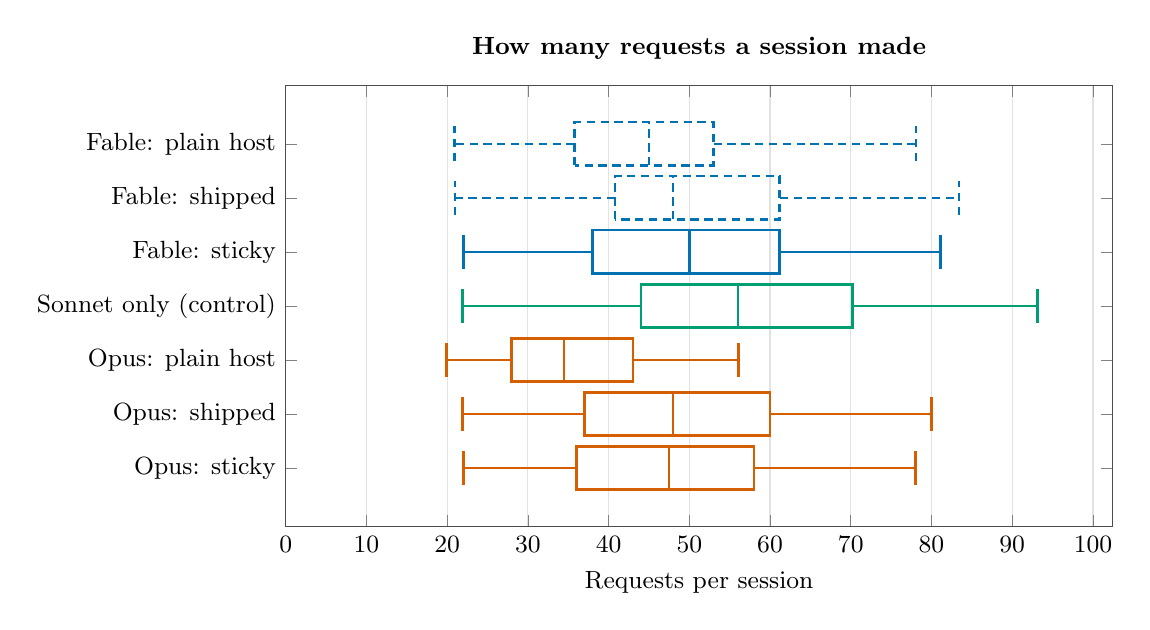
\begin{tikzpicture}
\begin{axis}[benchmark, scale only axis, width=10.5cm, height=5.6cm, xmin=0, xmajorgrids,
  ytick={1,...,\ReqBoxN}, yticklabels/.expanded={\ReqBoxLabels},
  xlabel={Requests per session}, title={How many requests a session made}, title style={font=\small\bfseries},
  boxplot/draw direction=x, every axis plot/.append style={line width=0.9pt}]
\addplot+[boxplot prepared={lower whisker=22.0, lower quartile=36.0, median=47.5, upper quartile=58.0, upper whisker=78.0}, color=okorange] coordinates {};
\addplot+[boxplot prepared={lower whisker=21.9, lower quartile=37.0, median=48.0, upper quartile=60.0, upper whisker=80.0}, color=okorange] coordinates {};
\addplot+[boxplot prepared={lower whisker=19.9, lower quartile=28.0, median=34.5, upper quartile=43.0, upper whisker=56.1}, color=okorange] coordinates {};
\addplot+[boxplot prepared={lower whisker=21.9, lower quartile=44.0, median=56.0, upper quartile=70.2, upper whisker=93.1}, color=okgreen] coordinates {};
\addplot+[boxplot prepared={lower whisker=22.0, lower quartile=38.0, median=50.0, upper quartile=61.2, upper whisker=81.1}, color=okblue] coordinates {};
\addplot+[boxplot prepared={lower whisker=21.0, lower quartile=40.8, median=48.0, upper quartile=61.2, upper whisker=83.4}, color=okblue] coordinates {};
\addplot+[boxplot prepared={lower whisker=20.9, lower quartile=35.8, median=45.0, upper quartile=53.0, upper whisker=78.1}, color=okblue] coordinates {};

\end{axis}
\end{tikzpicture}

\caption{Main-loop requests per session by kind of session: box from the 25th to the 75th percentile, line at
the median, whiskers from the 5th to the 95th percentile.}
\label{fig:requests}
\howtoread{Boxes further right made more requests for the same scripted work. Sonnet-heavy sessions sit to the
right of the plain Opus sessions, which is part of why routing cost more on Opus.}
\end{figure}

\begin{figure}[htbp]
\centering
\pgfplotslegendfromname{bandlegend}\par\smallskip
% Cost ratio by scripted session length (all splits, 95% CIs).
\begin{tikzpicture}
\begin{groupplot}[benchmark, group style={group size=2 by 1, horizontal sep=1.6cm},
  width=0.46\linewidth, height=5.2cm, xmin=0.5, xmax=3.5, xtick={1,2,3},
  xticklabels={{$\le$8},{9--12},{$\ge$13}}, xlabel={Scripted turns}, ymajorgrids, title style={font=\small\bfseries}]
\nextgroupplot[title={Fable host}, ylabel={Cost ratio vs plain host}, ymin=0.4, ymax=0.8,
  legend to name=bandlegend, legend columns=2, legend cell align=left,
  legend style={/tikz/every even column/.append style={column sep=10pt}}]
\addplot[only marks, mark=*, mark size=2.4pt, color=okblue, error bars/.cd, y dir=both, y explicit]
  table[x=x, y=r, y error minus=m, y error plus=p]{generated/data/band-fable-sticky.dat}; \addlegendentry{sticky}
\addplot[only marks, mark=square*, mark size=2.4pt, color=okorange, error bars/.cd, y dir=both, y explicit]
  table[x=x, y=r, y error minus=m, y error plus=p]{generated/data/band-fable-shipped.dat}; \addlegendentry{shipped (re-chooses each turn)}
\nextgroupplot[title={Opus host}, ymin=0.95, ymax=1.65]
\draw[black!60] (axis cs:0.5,1) -- (axis cs:3.5,1);
\addplot[only marks, mark=*, mark size=2.4pt, color=okblue, error bars/.cd, y dir=both, y explicit]
  table[x=x, y=r, y error minus=m, y error plus=p]{generated/data/band-opus-sticky.dat};
\addplot[only marks, mark=square*, mark size=2.4pt, color=okorange, error bars/.cd, y dir=both, y explicit]
  table[x=x, y=r, y error minus=m, y error plus=p]{generated/data/band-opus-shipped.dat};
\end{groupplot}
\end{tikzpicture}

\caption{Cost ratio by scripted session length, all splits, with 95\,\% intervals.}
\label{fig:band}
\howtoread{Flat rows mean the ratio does not depend on session length within 8--16 turns. Longer sessions moved
the Opus ratios slightly toward 1; on Fable the saving held at every length.}
\end{figure}

\section{The effort confound \texorpdfstring{\screen}{[screen]}}\label{sec:effort}

An external reviewer asked the question this campaign should have asked itself: when the sticky router chose Sonnet,
was its session the same as the plain-Sonnet control? It was not. Every routed Sonnet main request ran at
\emph{medium} reasoning effort (\RvEffMediumSticky\ of \RvEffStickyTotal\ requests in the sticky sessions that chose
Sonnet), because the bundle's composed configuration sets that start effort. The plain-Sonnet control sets no effort
(\RvEffNoneControl\ of \RvEffControlTotal\ requests), which the design document describes as the provider default,
high. So the comparison ``routed versus plain Sonnet'' also compares two effort levels.

\begin{table}[htbp]
\centering\small
\caption{Sticky sessions that chose Sonnet against the plain-Sonnet control on the same scenario and repetition
(geometric-mean cost ratio, 95\,\% scenario-cluster bootstrap intervals). Exploratory.}
\label{tab:effort}
\begin{tabular*}{\textwidth}{@{\extracolsep{\fill}}l r r r r@{}}
\toprule
 & \multicolumn{2}{c}{All scenarios} & \multicolumn{2}{c}{Test split} \\
\cmidrule(lr){2-3}\cmidrule(l){4-5}
Host & sessions & cost ratio & sessions & cost ratio \\
\midrule
Fable & \RvEffFableAllN & \RvEffFableAll\ (\RvEffFableAllCI) & \RvEffFableTestN & \RvEffFableTest\ (\RvEffFableTestCI) \\
Opus & \RvEffOpusAllN & \RvEffOpusAll\ (\RvEffOpusAllCI) & \RvEffOpusTestN & \RvEffOpusTest\ (\RvEffOpusTestCI) \\
\bottomrule
\end{tabular*}
\end{table}

\paragraph{What the medium-effort sessions did differently.} Against the control on the same scenarios, the sticky
sessions that ran on Sonnet made about \RvEffReqFable\,\% fewer requests on Fable (\RvEffReqOpus\,\% on Opus),
produced about \RvEffOutFable\,\% fewer output tokens (\RvEffOutOpus\,\%) and finished about \RvEffTimeFable\,\%
faster (\RvEffTimeOpus\,\%). Quality showed no detectable difference: turn-pass fraction moved by \RvEffDtpFable\
on Fable (95\,\% CI \RvEffDtpFableCI) and \RvEffDtpOpus\ on Opus (\RvEffDtpOpusCI). The sessions were not using the
read shortcut; the difference is the effort setting, possibly together with the bundle's own context, which this
data cannot separate.

\paragraph{Two further corrections.}
\begin{itemize}
  \item \textbf{The control ran in the Opus waves only.} Because it does not depend on the host, the plain-Sonnet
    control ran once per scenario and repetition, alongside the Opus sessions. Fable sessions and their Sonnet
    control started a median \RvSonnetWaveMedianH\ hours apart (at most \RvSonnetWaveMaxH\,h). The Opus result,
    with the control in the same wave, is about the same size, so timing is not what drives the gap.
  \item \textbf{Sticky sessions that kept the host cost more than the plain host.} The \RvStickyHostNFable\ sticky
    sessions per host that stayed on the host model cost \RvStickyHostFable\X\ the plain host on Fable and
    \RvStickyHostOpus\X\ on Opus. On Fable, sticky-on-Sonnet cost \RvEffVsAnchorFable\X\ the plain host where the
    control cost \RvCtlVsAnchorFable\X\ on the same scenarios; the dearer host-kept sessions offset most of that
    difference, which is why sticky and plain Sonnet look alike overall.
\end{itemize}

\subsection{Follow-up: plain Sonnet at medium versus default effort \texorpdfstring{\prereg}{[preregistered]}}\label{sec:effortfollow}

To separate the effort setting from the routing, a preregistered follow-up (effort-control-v1) ran plain Sonnet
twice on the \EcScen\ test scenarios, \EcReps\ repetitions each: once at the provider's default effort and once at
medium effort, nothing else changed. Each pair started together from the same frozen workspace with separate cache
nonces, so this comparison is concurrent. Intervals come from \EcResamples\ scenario-cluster resamples (seed
\EcSeed). The preregistered hypothesis (medium is cheaper, with non-inferior turn-pass fraction) was \EcHE.

\begin{table}[htbp]
\centering\small
\caption{Effort-control follow-up (evidence in the \texttt{2026-10-05-effort-control} directory). Cost rows are
geometric-mean ratios of tools-normalized session cost; below 1 means the first arm is cheaper.}
\label{tab:effortfollow}
\begin{tabular*}{\textwidth}{@{\extracolsep{\fill}}>{\raggedright\arraybackslash}p{0.5\textwidth} r r r@{}}
\toprule
Comparison & n & estimate & 95\,\% CI \\
\midrule
Medium / default effort, plain Sonnet (confirmatory, concurrent) & 46 pairs & 0.821 & 0.781--0.861 \\
Medium plain Sonnet / main-v1 sticky-on-Sonnet (exploratory, not concurrent) & 22 scenarios & 0.958 & 0.913--0.999 \\
\midrule
Turn-pass difference, medium minus default (unfiltered) & 46 pairs & $-$0.003 & $-$0.026 to 0.021 \\
\bottomrule
\end{tabular*}

\end{table}

\paragraph{Result.} Medium effort cost \EcRatio\X\ the default (95\,\% CI \EcCI), about \EcCutPct\,\% cheaper, and
was cheaper in \EcCheaperPairs\ of \EcPairs\ pairs. Turn-pass fraction moved by \EcQual\ (\EcQualCI): \EcQualVerdict\
at the \NIMarginPts-point margin. An exploratory comparison of medium plain Sonnet with the main-campaign sticky
sessions that ran on Sonnet (also at medium effort) gives \EcSecRatio\ (\EcSecCI, \EcSecN\ scenarios). Those
sessions ran on different dates, so this second comparison is not concurrent and has no decision rule. Read the
other way round, sticky-on-Sonnet cost about \EcSecGapPct\,\% more than medium plain Sonnet; that gap is within what
bundle behaviour or timing could produce.

\paragraph{Provenance caveat.} The follow-up's schedule and plan were created \EcScheduleBefore\ \emph{before} the
preregistration was committed (\code{\EcPreregSha}), and the first analysed session started \EcFirstAfter\ after it.
The design file and the analysis script were first committed in that same commit, so the evidence package cannot
prove that the working-tree copies used to build the schedule match the committed ones. No outcome data from the
analysed sessions existed before the commit. The follow-up cost \$\EcSpend\ (including a \$\EcPreflight\ preflight).

\begin{keyidea}
The effort setting alone explains most of the gap between sticky-on-Sonnet and plain Sonnet: in a concurrent test,
medium effort cost \EcRatio\X\ the default. On Fable~5.1 at the \cref{tab:prices} prices, the saving comes from
running the session on Sonnet at medium effort. On the Sonnet sessions the router's extra machinery did not help: sticky-on-Sonnet cost about \EcSecGapPct\,\% more
than plain Sonnet at medium effort (\EcSecRatio\ the other way round; exploratory, not concurrent), and the
\RvStickyHostNFable\ sessions per host that kept the host cost \RvStickyHostFableTwo\X\ (Fable) and
\RvStickyHostOpusTwo\X\ (Opus) the plain host. This campaign shows no benefit of this router beyond the decision to use
Sonnet. The finding also applies to anyone running plain Sonnet:
medium effort cut cost by about \EcCutPct\,\% with no detectable turn-pass loss on these \EcScen\ scenarios (\RvDocsTest\ docs, \RvExplainTest\ explain, \RvReviewTest\ review); the main campaign
hints at a loss on docs, explain and review work (sticky-on-Sonnet at medium minus the default-effort control:
\RvKTDtp\ [\RvKTDtpCI] on those \RvKTN\ scenarios against \RvRestDtp\ [\RvRestDtpCI] on the rest; post hoc, and
confounded with the bundle's context) that the follow-up is too small to settle.
\end{keyidea}


\part{Implications}\label{part:implications}
\section{What it means}\label{sec:recs}

\begin{keyidea}
\textbf{Fable~5.1 at the \cref{tab:prices} prices: move the session to Sonnet, and decide once.} On Fable 5.1
at the Table~\ref{tab:prices} prices, sticky routing saved about \CfFableStickySaving\,\% (typical per-session saving: geometric mean of
per-pair cost ratios; actual spend fell \RvSpendCutAll\,\% over all \NScenarios\ scenarios, from \$\RvSpendAnchor\ to
\$\RvSpendSticky\ per session, and \RvSpendCutTest\,\% on the test split), with turn-pass
fraction inside the preregistered \NIMarginPts-point margin on the \NTest\ test scenarios. Across all
\QAllScen\ scenarios that margin was not shown for sticky (\QAllFableSticky, CI \QAllFableStickyCI), and
routed Fable arms passed the final hidden tests \FinalGapLow--\FinalGapHigh\ points less often
(exploratory). The sticky policy cost less than the shipped one (\HThreeFable\X\ on Fable, \HThreeOpus\X\ on
Opus); the preregistered test was only that sticky costs no more than shipped. At these prices the saving is
Sonnet-at-medium relative to the host at its default effort; the host at medium effort was not measured
(\cref{sec:limits}).
\end{keyidea}

\paragraph{How much of the saving is the router, and how much the effort setting.} An earlier draft read the data
as supporting ``use Sonnet'' as much as ``use the router''. That reading is withdrawn. When the sticky router chose
Sonnet it ran every main request at medium reasoning effort, while the plain-Sonnet control used the provider
default; those sticky sessions cost \RvEffFableAll\X\ (Fable) and \RvEffOpusAll\X\ (Opus) the control on the same
scenarios, with no detectable quality difference (\cref{sec:effort}). So part of the routing saving is the effort
setting, which a ``just use Sonnet'' deployment would also get if it set the same effort. On Fable the near-equality
of sticky (\CfFableStickyPair\X) and plain Sonnet (\CfFableSonnetPair\X) is two effects cancelling: medium-effort
Sonnet is cheaper than the control, while the \RvStickyHostNFable\ sticky sessions that kept the host cost
\RvStickyHostFable\X\ the plain host. The per-1,000 figures (\$\SavFableSticky\ for sticky, \$\SavFableSonnet\ for
Sonnet) are mean-difference (spend) measures. The judge's own calls are not in the session costs
(\cref{sec:design}); by an estimate from another study they would add about \JudgeShippedCents\ cents per shipped
session, which does not change these conclusions. Then a follow-up designed in advance (its plan was committed \EcFirstAfter\ before its first analysed session;
\cref{sec:effortfollow}) showed that medium effort alone makes plain Sonnet cost \EcRatio\X\ the default (95\,\% CI \EcCI),
run concurrently on the \EcScen\ test scenarios. So the effort setting alone explains most of the
sticky-versus-plain-Sonnet gap; read the other way round, sticky-on-Sonnet cost about \EcSecGapPct\,\% more than medium
plain Sonnet (\EcSecRatio; exploratory and not concurrent), within what bundle behaviour or timing could produce. The
practical reading: on Fable~5.1 at the \cref{tab:prices} prices, the saving comes from running the session on Sonnet at
medium effort. On the Sonnet sessions the router's extra machinery did not help: sticky-on-Sonnet cost about \EcSecGapPct\,\% more
than plain Sonnet at medium effort (\EcSecRatio\ the other way round; exploratory, not concurrent), and the
\RvStickyHostNFable\ sessions per host that kept the host cost \RvStickyHostFableTwo\X\ (Fable) and
\RvStickyHostOpusTwo\X\ (Opus) the plain host. This campaign shows no benefit of this router beyond the decision to use
Sonnet. Anyone already running plain Sonnet can take the effort result on its own: medium effort cut
cost by about \EcCutPct\,\% with no detectable turn-pass loss on these \EcScen\ scenarios (\RvDocsTest\ docs, \RvExplainTest\ explain, \RvReviewTest\ review); the main campaign
hints at a loss on docs, explain and review work (sticky-on-Sonnet at medium minus the default-effort control:
\RvKTDtp\ [\RvKTDtpCI] on those \RvKTN\ scenarios against \RvRestDtp\ [\RvRestDtpCI] on the rest; post hoc, and
confounded with the bundle's context) that the follow-up is too small to settle.

\begin{keyidea}
\textbf{Opus~5.5 at the \cref{tab:prices} prices: do not route to Sonnet.} Opus's cache reads are cheaper than
Sonnet's, and Sonnet needed more requests for the same scripted work, so every routing arm cost more:
\CfOpusStickyExtra--\CfOpusSonnetExtra\,\% more in the pair reading and
\CfOpusStickyArmExtra--\CfOpusSonnetArmExtra\,\% in the arm reading. The plain host is the right default
\emph{at these prices}. If Opus cache reads cost about \$\BEStickyPair\ rather than \$\PriceOpusRead\ per
million tokens, sticky routing would roughly break even (\cref{sec:breakeven}). The Opus result does not depend on
the effort setting: sticky sessions that ran Sonnet at medium effort still cost \RvEffVsAnchorOpusTwo\X\ (95\,\% CI
\RvEffVsAnchorOpusCI) the plain Opus host.
\end{keyidea}

\paragraph{Quality by task type.} The aggregate Fable sticky quality hides a split (\cref{tab:taskfable}):
\RgNTaskFail\ of \RgNTask\ task types fall below the \NIMarginPts-point margin (\RgTaskFailList), \RgNTaskThreeX\
of them by about three times, and they are among the largest savers. The aggregate passes because bugfix and
mixed scenarios are numerous. Routing only the task types that hold their quality could avoid most of the loss;
that is a hypothesis for the next campaign, not a finding.

\paragraph{The judge.} Keep Jev as the default judge. The post-hoc Cloudflare Clef judge matched its accuracy but
was \ClClefCostXLow--\ClClefCostXHigh\X\ the cost per decision and about three times slower from this machine; it is
worth re-testing if it can be hosted close to the agent or if its measured latency improves. Clef-Flash was cheaper
but less accurate (\cref{sec:clef}). Neither was part of the paired campaign. Taken together, the evidence does not
establish the value of the decision-judge machinery itself: no judge met the usefulness rule on real decisions
(\cref{sec:traces}), and the router showed no benefit beyond the decision to use Sonnet (\cref{sec:effort}). Jev
remains the best of the judges tested.

\paragraph{Caching guidance (hypotheses).} The mechanisms in \cref{sec:caching,sec:composition} suggest the
following for other hosts and prices. They are hypotheses drawn from two hosts on one provider, not tested
findings:
\begin{itemize}
  \item \textbf{Compare price per token class, not price per token.} A model that is cheaper on input and
    output may be dearer in a long conversation if its cache reads cost more.
  \item \textbf{Every switch re-writes the history.} Switching less often, ideally once at the start, should
    avoid most rebuild cost.
  \item \textbf{Count requests, not just tokens.} The cheaper model made more requests for the same scripted
    work here; that volume, not only the price, decided the Opus result.
  \item \textbf{Pauses matter.} An idle gap longer than the cache lifetime makes the next request pay to
    write the history again, on any model.
  \item \textbf{Measure with isolation.} Give every measured session a private cache key (a nonce), and never
    start two identical requests at the same instant.
\end{itemize}

\paragraph{How to use the numbers.} For a deployment that looks like this campaign, use the measured savings
per 1,000 sessions in \cref{tab:per1000,tab:per1000full}. The savings model is suitable for a pooled
forecast over a similar mix, with its interval; do not use its per-host or per-task figures
(\cref{sec:modellimits}).

\paragraph{What to measure next.}
\begin{itemize}
  \item \textbf{Longer sessions.} Real sessions often run for many dozens of turns; these ran at most
    \MaxTurns.
  \item \textbf{Real traffic.} Scripted users do not wait, wander or abandon sessions as people do.
  \item \textbf{A production measure mode.} Routed and unrouted paths cannot both run in one live session,
    but each production session can carry the model's prediction and interval, and sampled offline replays
    can provide fresh paired measurements.
  \item \textbf{Other hosts and providers.} The direction of the result depends on the price table; a new
    host model needs its own measurement, or at least a check of its read and write prices against Sonnet's.
  \item \textbf{The final-pass signal.} A larger sample would settle whether the small excess of final-test
    losses on routed Fable arms is real (\cref{sec:finalpass}).
\end{itemize}

\section{Limitations and threats to validity}\label{sec:limits}

\begin{itemize}
  \item \textbf{Scripted, synthetic sessions.} The \NScenarios\ scenarios are fixed scripts of
    \MinTurns--\MaxTurns\ turns with automatic checks. Real users react to answers, pause irregularly and
    hold much longer conversations.
  \item \textbf{The judge's own cost is not measured.} Session costs exclude the routing judge's calls
    (\cref{sec:design}).
  \item \textbf{Two hosts, one provider.} The conclusions are tied to these models and this price table;
    they do not transfer to other providers or price changes without new measurement.
  \item \textbf{A price table, not invoices.} Costs are tokens times list prices from the bundle's own table
    (verified \RatesVerified). They match the provider's per-request cost field exactly, but that field uses
    the same table, so the match checks token counting, not prices; discounts and batch pricing are not
    modelled.
  \item \textbf{The Opus result depends on one price.} At the table's \$\PriceOpusRead\ per million cached
    Opus tokens, routing cost more; re-pricing the recorded tokens, sticky reaches parity at about
    \$\BEStickyPair\ (pair reading) or \$\BEStickyArm\ (arm reading), and at \$\RateForty\ sticky would cost
    \BEStickyForty\X\ the plain host (\cref{tab:breakeven}). The Opus conclusion is about Opus~5.5 at these
    prices, not about ``Opus-class'' models in general.
  \item \textbf{The primary filter selects on an outcome.} The pair reading keeps pairs whose arm did at
    least as well as its anchor. That conditions on something the treatment affects. The arm reading, which
    keeps every cost-valid pair, gives the same verdicts; the filter raises the sticky and shipped ratios by
    \FilterLiftLow\ to \FilterLiftHigh\ (\cref{tab:primary}).
  \item \textbf{Uncommitted harness code during the run.} The runner that executed the campaign was
    working-tree code, committed only afterwards (\code{\HarnessSha}). The agent under test was frozen at the
    preregistration commit, and re-extraction with the committed harness reproduces the rows byte for byte,
    but the exact runner code was not under version control while it ran.
  \item \textbf{The estimator was written after the data.} The preregistration fixed hypotheses, thresholds,
    split and decision rule; the confirmatory script that fixed resamples, seed, the quality filter and the
    verdict rule was committed about \ConfirmAfterMin\ minutes after the campaign finished, when exploratory
    summaries over all scenarios existed. The analysis also resolved \NDeviations\ ambiguities or mismatches
    in the preregistration (\cref{sec:deviations}); only the two non-inferiority readings and the bootstrap
    seed were varied in sensitivity checks.
  \item \textbf{The Opus A/A ratio is not centred on 1, for reasons we cannot explain.} Two identical Opus
    sessions differed by about \AAOpusPct\,\% on average (\AAOpus, \AAOpusCI). The bias is not associated with
    start offset (\cref{sec:aa}). Removing a bias of that size would put the Opus ratios at about
    \OpusAdjLow--\OpusAdjHigh; the verdicts hold.
  \item \textbf{Reasoning effort differs between the routed arms and the Sonnet control.} Routed Sonnet ran at
    medium effort and the plain-Sonnet control at the provider default, so part of the routing saving is the
    effort setting (\cref{sec:effort}). The control also ran only in the Opus waves, hours away from the Fable
    sessions it is compared with.
  \item \textbf{No held-out docs scenario.} All \RvDocsTrain\ docs scenarios are in the training split; the test
    split has \RvDocsTest\ docs, \RvExplainTest\ explain and \RvReviewTest\ review scenarios (\cref{tab:tasksplit}).
    Docs results, including the Opus docs exception, rest on training data only.
  \item \textbf{Inferred failure causes.} For \NFailedInferred\ of the \NFailed\ failed attempts the cause
    was inferred from timing, not recorded. Failed attempts were rerun as whole waves, so they cannot bias
    the accepted data, but the failure accounting for them is probable, not proven.
  \item \textbf{One shared API key.} Isolation between arms relies on the per-session nonce and the audit
    (\AuditFlagged\ flagged sessions), not on separate keys.
  \item \textbf{Quality is near the margin.} Fable sticky passed the turn-pass margin on the test split by
    \QFableStickyMarginGap; over all scenarios the margin was not shown, and routed Fable arms passed the
    final hidden tests \FinalGapLow--\FinalGapHigh\ points less often (exploratory, \cref{sec:finalpass}).
  \item \textbf{The savings model is additive.} It assumes the same arm and task effects on both hosts and
    misfits per-host cells (\cref{sec:modellimits}).
\end{itemize}

\section{Reproducibility}\label{sec:repro}

\paragraph{Evidence.} Everything is in \path{docs/evidence/2026-10-02-paired-campaign/}:
\begin{itemize}
  \item \path{data/} and its \path{DATA-DICTIONARY.md}, which documents every field: \NSessions\ session
    rows, \NTurns\ turn rows, \NRequests\ request rows and \NPairs\ pair rows;
  \item \path{confirm/}: the preregistered confirmatory analysis (\path{confirm.json}, \path{CONFIRM.md});
  \item \path{model/}: the savings model, its summaries and its test-split predictions;
  \item \path{campaign/}: schedule, state, ledger, sticky decisions and \path{FAILURES.md};
  \item \path{prereg/}: the preregistration, the split and \path{PROVENANCE.md};
  \item \path{pilot/} and \path{reproduce/} (commands, versions, price table, spend).
\end{itemize}
The agent under test was frozen at commit \code{\BuildSha} (the preregistration commit) in every session.

\paragraph{The effort-control follow-up.} Its evidence directory is:
\begin{center}\path{docs/evidence/2026-10-05-effort-control/}\end{center}
It holds \path{summary.json}, \path{RESULT.md}, \path{result/effort-result.json}, \path{prereg/PROVENANCE.md} and the
rows in \path{data/}. The follow-up ran \EcPairs\ concurrent pairs on the \EcScen\ test scenarios and cost
\$\EcSpend\ (including a \$\EcPreflight\ preflight), so the measured spend across the main campaign and the
follow-up is \$\SpendWithFollowup. The Fable effort follow-up
(\path{docs/evidence/2026-10-06-effort-control-fable/}; preregistration \code{\EfPreregSha}) cost \$\EfSpend. Its preregistration was committed as \code{\EcPreregSha}; the timing caveat is
in \cref{sec:effortfollow}.

\paragraph{Re-running the analysis.} No model call is needed. From the published rows, the savings model
re-fits byte for byte:
\begin{lstlisting}
E=docs/evidence/2026-10-02-paired-campaign
S=$(mktemp -d); mkdir "$S/rows"
ln -s "$PWD/$E/data/sessions.jsonl" "$PWD/$E/data/pairs.jsonl" "$S/rows/"
nice -n 10 python3 evals/paired_model.py all "$S" --engine fallback
nice -n 10 python3 evals/paired_confirm.py "$S"
\end{lstlisting}
Re-extracting the rows themselves needs the raw campaign tree and per-session event files, which are not
published; on the machine that ran the campaign, \code{evals/paired.py rows} reproduces them byte for byte.

\paragraph{This document.} The source is in \path{docs/papers/2026-10-02-paired-measurement/}. Running
\code{make} there runs \code{build\_assets.py}, which reads only the committed files listed at its top
(including the earlier caching survey from the \code{eval/judge-realistic} branch) and writes every number
(\path{generated/numbers.tex}), table, plotted datum and label position, then builds the PDF. No number in
the text is typed by hand. The script recovers the price table from the request rows themselves and checks
that it prices every request to within \PriceResidual\ dollars. \code{make check} re-checks the figures'
geometry on the built PDF: every scatter label nearest its own marker, every legend above its plot, and no
overlapping text anywhere.


\appendix
\section{Glossary}\label{app:glossary}

\begin{description}[leftmargin=1.2em,style=nextline,itemsep=3pt]
  \item[A/A] Running the same configuration twice on the same task to measure how much two identical
    sessions differ by chance.
  \item[Anchor] The plain host model with no routing; every other arm is compared with it.
  \item[Arm] One configuration of the agent in the experiment: anchor, aa, shipped, sticky or sonnet.
  \item[Bootstrap (scenario-cluster)] Estimating uncertainty by resampling whole scenarios with replacement
    many times and recomputing the result each time.
  \item[Cache read, cache write] Re-using a prefix already in the provider's cache is billed as a cheap
    read; storing a new prefix is billed as a more expensive write.
  \item[Cache rebuild] Re-writing the conversation history to a new model's cache after a switch.
  \item[Confidence interval (95\,\%)] The range of values consistent with the data; built so that over
    many repeats of the study it contains the true value 95\,\% of the time.
  \item[Confirmatory] A result that tests a hypothesis fixed in advance, on data held out for that purpose.
  \item[Exploratory] Any other result: useful for understanding, not for confirming.
  \item[Geometric mean] The average of ratios that treats ``twice'' and ``half'' symmetrically: the
    exponential of the mean of the log ratios.
  \item[Host model] The large model an agent session normally runs on (here Fable 5.1 or Opus 5.5).
  \item[McNemar's test] A test for paired yes/no outcomes that looks only at the pairs where the two sides
    disagree.
  \item[Non-inferior] Not worse than the baseline by more than a set margin (here \NIMarginPts\ points of
    turn-pass fraction).
  \item[Nonce] A unique string at the start of each session's system prompt that makes its cache entries
    private.
  \item[Pair] A routed session and the anchor session on the same scenario, repetition and host.
  \item[Preregistration] A dated, committed plan of hypotheses, analysis and decision rules made before
    the data exist.
  \item[Prediction interval (90\,\%)] The range a new observation is expected to fall in 90\,\% of the time.
  \item[Routing] Sending some of a session's requests to a different, usually cheaper, model.
  \item[Shipped] The bundle's default routing policy; it re-chooses its model at the start of each turn and never
    switches in the middle of a turn.
  \item[Sticky] A policy that chooses the model once, from the first prompt, and never switches.
  \item[Tools-normalized cost] Cost with the shared tool definitions on a session's first request priced as
    a cache read, as they would usually be in production.
  \item[Turn-pass fraction] The share of a session's turns whose automatic checks passed.
  \item[Wave] All arms of one scenario, repetition and host, started together from the same workspace.
\end{description}

\section{Additional tables}\label{app:tables}

\begin{table}[htbp]
\centering\small
\caption{Savings-model check by arm and host, test split: prediction-interval coverage and the observed total
saving against its predicted 90\,\% interval.}
\label{tab:modelcheck}
\begin{tabular*}{\textwidth}{@{\extracolsep{\fill}}l r r r r r c@{}}
\toprule
Arm / host & pairs & coverage (log) & coverage (\$) & observed total & 90\,\% PI of total & inside \\
\midrule
shipped / Fable & 46 & 0.957 & 0.978 & \$85.01 & 64.78 to 121.24 & \ok \\
shipped / Opus & 46 & 1.000 & 0.978 & \$$-$31.48 & $-$45.42 to $-$20.50 & \ok \\
sonnet / Fable & 46 & 0.935 & 0.935 & \$94.95 & 39.53 to 95.29 & \ok \\
sonnet / Opus & 46 & 0.957 & 0.826 & \$$-$46.80 & $-$57.41 to $-$29.04 & \ok \\
sticky / Fable & 46 & 0.913 & 0.935 & \$99.82 & 70.67 to 132.14 & \ok \\
sticky / Opus & 46 & 1.000 & 0.957 & \$$-$21.15 & $-$42.03 to $-$16.57 & \ok \\
\bottomrule
\end{tabular*}

\end{table}

\begin{table}[htbp]
\centering\small
\caption{A/A noise floor: second plain-host session against the first. ``SD'' is the standard deviation of
the log ratio per pair and per single session.}
\label{tab:aa}
\begin{tabular*}{\textwidth}{@{\extracolsep{\fill}}l l r r r r r l@{}}
\toprule
Split & Host & pairs & ratio & 95\,\% CI & SD (pair) & SD (session) & centred \\
\midrule
all & Fable & 28 & 0.968 & 0.94--1.00 & 0.097 & 0.069 & yes \\
all & Opus & 27 & 1.049 & 1.01--1.09 & 0.103 & 0.073 & no \\
all & both & 55 & 1.007 & 0.97--1.04 & 0.107 & 0.076 & yes \\
test & Fable & 9 & 0.957 & 0.91--1.01 & 0.082 & 0.058 & yes \\
test & Opus & 9 & 1.035 & 0.96--1.10 & 0.103 & 0.073 & yes \\
test & both & 18 & 0.995 & 0.94--1.05 & 0.099 & 0.070 & yes \\
\bottomrule
\end{tabular*}

\end{table}

\begin{table}[htbp]
\centering\small
\caption{Interim and final cost ratios behind \cref{fig:interim}.}
\label{tab:interim}
\begin{tabular*}{\textwidth}{@{\extracolsep{\fill}}l l r r r r r@{}}
\toprule
Host & Arm & pilot & interim & final train (95\,\% CI) & final test (95\,\% CI) & confirmatory \\
\midrule
Fable 5.1 & sticky & 0.53 & 0.60 & 0.571 (0.51--0.64) & 0.537 (0.48--0.61) & \CfFableStickyPair \\
Fable 5.1 & shipped & 0.65 & 0.70 & 0.640 (0.58--0.70) & 0.618 (0.55--0.70) & \CfFableShippedPair \\
Fable 5.1 & sonnet & 0.62 & 0.58 & 0.585 (0.54--0.63) & 0.590 (0.53--0.66) & \CfFableSonnetPair \\
Opus 5.5 & sticky & 1.46 & 1.11 & 1.199 (1.11--1.30) & 1.203 (1.09--1.33) & \CfOpusStickyPair \\
Opus 5.5 & shipped & 1.35 & 1.12 & 1.224 (1.13--1.33) & 1.321 (1.19--1.47) & \CfOpusShippedPair \\
Opus 5.5 & sonnet & 1.66 & 1.36 & 1.447 (1.31--1.60) & 1.457 (1.29--1.67) & \CfOpusSonnetPair \\
\bottomrule
\end{tabular*}

\end{table}

\begin{table}[htbp]
\centering\small
\caption{Cost ratio by pause pattern, all splits (95\,\% CI). Exploratory.}
\label{tab:slicegap}
\begin{tabular*}{\textwidth}{@{\extracolsep{\fill}}l l r r @{}}
\toprule
Host & Arm & no long gap & two long gaps \\
\midrule
Fable 5.1 & sticky & 0.56 (0.51--0.63) & 0.55 (0.48--0.64) \\
 & shipped & 0.63 (0.57--0.69) & 0.64 (0.57--0.73) \\
 & sonnet & 0.59 (0.55--0.65) & 0.57 (0.53--0.62) \\
\addlinespace[3pt]
Opus 5.5 & sticky & 1.21 (1.11--1.32) & 1.18 (1.07--1.30) \\
 & shipped & 1.30 (1.19--1.42) & 1.17 (1.08--1.28) \\
 & sonnet & 1.47 (1.33--1.63) & 1.41 (1.27--1.56) \\
\bottomrule
\end{tabular*}

\end{table}

\begin{table}[htbp]
\centering\small
\caption{Cost ratio by scripted session length, all splits (95\,\% CI). Exploratory.}
\label{tab:sliceturns}
\begin{tabular*}{\textwidth}{@{\extracolsep{\fill}}l l r r r @{}}
\toprule
Host & Arm & $\le$8 turns & 9--12 turns & $\ge$13 turns \\
\midrule
Fable 5.1 & sticky & 0.54 (0.49--0.60) & 0.58 (0.50--0.67) & 0.56 (0.47--0.69) \\
 & shipped & 0.64 (0.56--0.73) & 0.64 (0.56--0.73) & 0.62 (0.56--0.69) \\
 & sonnet & 0.63 (0.54--0.73) & 0.57 (0.52--0.63) & 0.57 (0.53--0.61) \\
\addlinespace[3pt]
Opus 5.5 & sticky & 1.25 (1.11--1.44) & 1.22 (1.11--1.34) & 1.11 (1.01--1.24) \\
 & shipped & 1.36 (1.18--1.55) & 1.26 (1.15--1.38) & 1.14 (1.04--1.24) \\
 & sonnet & 1.57 (1.34--1.85) & 1.44 (1.29--1.61) & 1.33 (1.18--1.50) \\
\bottomrule
\end{tabular*}

\end{table}

\subsection*{Raw cost basis}\label{sec:rawbasis}
Without the tools normalization the confirmatory ratios barely move: Fable sticky \RawFableSticky\ (against
\CfFableStickyPair) and Opus sticky \RawOpusSticky\ (against \CfOpusStickyPair).

\subsection*{Deviations from the preregistration}\label{sec:deviations}
Verbatim from \path{confirm/confirm.json}:
{\small\begin{enumerate}[leftmargin=1.4em]
\item Coverage bounds: paired\_model.py (PREREG constant) and MODEL.md use 0.83-0.97 plus a calibration-slope check 0.7-1.3; the preregistration says [0.80, 0.97] and has no slope check. The verdict here uses [0.80, 0.97]; the slope and paired\_model's own checks are reported, not used.
\item Coverage outcome: the prereg does not say which outcome's PI coverage is checked; both the log-ratio and the delta-\$ model coverage must be in bounds here (stricter of the two readings).
\item Primary-endpoint restriction is ambiguous (pair-level vs arm-level non-inferiority). Pair-level matches the text ('among pairs where ...') and is primary; arm-level is reported alongside. Pair-level filtering conditions on a post-treatment outcome and in this design keeps only pairs with delta\_turn\_pass >= 0 (steps are >= 1/16). [This report treats both readings as co-primary.]
\item Non-inferiority comparison: paired\_model uses lower bound >= -0.05; the prereg says > -0.05, used here.
\item 'Lower bound' for Quality is the 2.5th percentile (two-sided 95\% bootstrap CI), consistent with the 95\% CIs of the primary endpoint; the prereg does not state the level for this bound.
\item 'Contradicted' is not defined in the prereg; defined here, before looking at test numbers, as the 95\% CI lying entirely on the other side of the same preregistered threshold.
\item H3 restriction: the prereg does not say which pairs enter the sticky/shipped ratio; pair reading keeps triplets where both sticky and shipped are pair-level non-inferior to the shared anchor; arm reading keeps all.
\item Decision rule: 'H3 holds' is read as H3 as a whole (both hosts), and 'H1 holds' as both sticky and shipped.
\item Model engine: statsmodels is not installed, so the fit used paired\_model's numpy fallback (method-of-moments variance components + feasible GLS), not REML MixedLM. The model is the existing model.json (train only, fit-boot 400, seed 0); the PI check re-runs predict with its on-disk seed/draws and with seed 20261002 as a sensitivity check.
\item Bootstrap: 10,000 resamples, seed 20261002 (per analysis instructions; the prereg names 20261002 as the split seed).
\end{enumerate}
}

Three further points, not listed in \path{confirm.json}:
\begin{enumerate}[leftmargin=1.4em,resume]
  \item \textbf{The estimator was written after the data.} \code{evals/paired\_confirm.py} (commit
    \code{\ConfirmSha}) was committed about \ConfirmAfterMin\ minutes after the campaign finished, when the
    exploratory all-scenario summaries in \path{model/} already existed. It fixed the bootstrap (\Boot\
    resamples, seed \BootSeed), the pair-level filter and the verdict rule, including ``contradicted''.
  \item \textbf{What counts as a savings claim.} Only arm and host cells whose own cost interval shows a saving
    (upper end below 1) are treated as savings claims and tested for quality; on this data those are the three
    Fable cells.
  \item \textbf{The design document's stricter model check also passes.} The design document asked for
    coverage between \DesignCovLow\ and \DesignCovHigh\ and a calibration slope between \DesignSlopeLow\ and
    \DesignSlopeHigh; the model reached \MCCovLog\ (log ratio), \MCCovUSD\ (dollars) and slope \MCSlope.
\end{enumerate}

{\small\begin{xltabular}{\textwidth}{@{}l l l r r r c@{}}
\caption{Savings per 1,000 sessions by host, task type and arm, measured (all splits) and as predicted by the preregistered model. Positive numbers are money saved, negative numbers money lost. Exploratory.}\label{tab:per1000full}\\
\toprule
Host & Task type & Arm & measured / 1,000 & 90\,\% range & model / 1,000 & model inside \\
\midrule
\endfirsthead
\multicolumn{7}{@{}l}{\small\emph{(continued)}}\\
\toprule
Host & Task type & Arm & measured / 1,000 & 90\,\% range & model / 1,000 & model inside \\
\midrule
\endhead
\bottomrule
\endlastfoot
Fable 5.1 & bugfix & sticky & 1{,}346 & 848 to 1{,}882 & 222 & \no \\
 &  & shipped & 797 & 385 to 1{,}232 & 64 & \no \\
 &  & sonnet & 871 & 486 to 1{,}270 & $-$352 & \no \\
\addlinespace[2pt]
 & feature & sticky & 2{,}183 & 1{,}095 to 3{,}188 & 2{,}820 & \ok \\
 &  & shipped & 2{,}019 & 1{,}254 to 2{,}784 & 2{,}604 & \ok \\
 &  & sonnet & 2{,}895 & 2{,}350 to 3{,}484 & 2{,}031 & \no \\
\addlinespace[2pt]
 & mixed & sticky & 2{,}020 & 1{,}241 to 2{,}720 & 2{,}771 & \no \\
 &  & shipped & 1{,}941 & 1{,}532 to 2{,}355 & 2{,}553 & \no \\
 &  & sonnet & 2{,}405 & 2{,}065 to 2{,}740 & 1{,}975 & \no \\
\addlinespace[2pt]
 & docs & sticky & 2{,}615 & 2{,}045 to 3{,}326 & 3{,}661 & \no \\
 &  & shipped & 2{,}263 & 1{,}924 to 2{,}683 & 3{,}445 & \no \\
 &  & sonnet & 2{,}246 & 1{,}711 to 3{,}049 & 2{,}871 & \ok \\
\addlinespace[2pt]
 & explain & sticky & 2{,}315 & 1{,}945 to 2{,}703 & 2{,}877 & \no \\
 &  & shipped & 2{,}244 & 1{,}671 to 2{,}723 & 2{,}743 & \no \\
 &  & sonnet & 2{,}367 & 2{,}058 to 2{,}668 & 2{,}388 & \ok \\
\addlinespace[2pt]
 & review & sticky & 3{,}007 & 2{,}469 to 3{,}509 & 3{,}853 & \no \\
 &  & shipped & 3{,}011 & 2{,}456 to 3{,}522 & 3{,}613 & \no \\
 &  & sonnet & 2{,}389 & 1{,}863 to 2{,}797 & 2{,}977 & \no \\
\addlinespace[2pt]
 & all tasks & sticky & 1{,}980 & 1{,}577 to 2{,}368 & 2{,}531 & \no \\
 &  & shipped & 1{,}754 & 1{,}481 to 2{,}032 & 2{,}314 & \no \\
 &  & sonnet & 2{,}090 & 1{,}834 to 2{,}340 & 1{,}739 & \no \\
\addlinespace[2pt]
\midrule
Opus 5.5 & bugfix & sticky & $-$1{,}037 & $-$1{,}339 to $-$752 & $-$1{,}112 & \ok \\
 &  & shipped & $-$1{,}240 & $-$1{,}501 to $-$996 & $-$1{,}176 & \ok \\
 &  & sonnet & $-$1{,}948 & $-$2{,}300 to $-$1{,}626 & $-$1{,}347 & \no \\
\addlinespace[2pt]
 & feature & sticky & $-$574 & $-$776 to $-$385 & $-$501 & \ok \\
 &  & shipped & $-$490 & $-$708 to $-$301 & $-$590 & \ok \\
 &  & sonnet & $-$1{,}099 & $-$1{,}376 to $-$839 & $-$824 & \no \\
\addlinespace[2pt]
 & mixed & sticky & $-$303 & $-$511 to $-$104 & $-$537 & \no \\
 &  & shipped & $-$401 & $-$597 to $-$212 & $-$626 & \no \\
 &  & sonnet & $-$815 & $-$1{,}257 to $-$458 & $-$862 & \ok \\
\addlinespace[2pt]
 & docs & sticky & 264 & 99 to 500 & $-$159 & \no \\
 &  & shipped & 162 & 1 to 321 & $-$248 & \no \\
 &  & sonnet & $-$129 & $-$458 to 185 & $-$482 & \no \\
\addlinespace[2pt]
 & explain & sticky & 341 & 227 to 434 & 150 & \no \\
 &  & shipped & 235 & 14 to 397 & 95 & \ok \\
 &  & sonnet & 242 & 66 to 399 & $-$50 & \no \\
\addlinespace[2pt]
 & review & sticky & $-$425 & $-$838 to $-$29 & $-$260 & \ok \\
 &  & shipped & $-$642 & $-$900 to $-$393 & $-$358 & \no \\
 &  & sonnet & $-$1{,}193 & $-$1{,}568 to $-$830 & $-$618 & \no \\
\addlinespace[2pt]
 & all tasks & sticky & $-$489 & $-$639 to $-$342 & $-$625 & \ok \\
 &  & shipped & $-$588 & $-$726 to $-$456 & $-$714 & \ok \\
 &  & sonnet & $-$1{,}096 & $-$1{,}329 to $-$881 & $-$949 & \ok \\
\end{xltabular}
}

{\small\begin{xltabular}{\textwidth}{@{}l l l l r r l@{}}
\caption{The \NScenarios\ scenarios, their family, task type, language, number of scripted turns, number of long gaps and preregistered split.}\label{tab:scenarios}\\
\toprule
Scenario & family & task type & language & turns & long gaps & split \\
\midrule
\endfirsthead
\multicolumn{7}{@{}l}{\small\emph{(continued)}}\\
\toprule
Scenario & family & task type & language & turns & long gaps & split \\
\midrule
\endhead
\bottomrule
\endlastfoot
commander-docs & knowledge & docs & javascript & 13 & 2 & train \\
debug-triage & knowledge & mixed & javascript & 11 & 0 & test \\
fastrand-explain & knowledge & explain & rust & 9 & 0 & test \\
fatihcolor-docs & knowledge & docs & go & 8 & 0 & train \\
fd-cli-docs & knowledge & docs & rust & 16 & 2 & train \\
filelock-explain & knowledge & explain & python & 9 & 0 & test \\
gohumanize-review & knowledge & review & go & 12 & 0 & train \\
humanize-review & knowledge & review & python & 12 & 2 & test \\
kac-docs & knowledge & docs & ruby & 14 & 0 & train \\
ms-review & knowledge & review & javascript & 8 & 0 & train \\
nanoid-explain & knowledge & explain & javascript & 10 & 0 & train \\
pflag-mixed & knowledge & mixed & go & 15 & 0 & train \\
semver-review & knowledge & review & rust & 10 & 0 & test \\
yamllint-mixed & knowledge & mixed & python & 14 & 2 & train \\
api-docs & mixed & mixed & python & 16 & 2 & test \\
arch-explain & mixed & mixed & python & 16 & 0 & train \\
changelog-gen & mixed & mixed & python & 12 & 0 & train \\
config-matrix & mixed & mixed & python & 12 & 0 & train \\
deps-audit & mixed & mixed & python & 8 & 0 & train \\
discrepancy-docs & mixed & mixed & python & 16 & 2 & test \\
docstring-audit & mixed & mixed & python & 12 & 0 & test \\
expense-anomaly & mixed & mixed & python & 12 & 2 & train \\
hr-salary-qa & mixed & mixed & python & 16 & 0 & train \\
log-incident & mixed & mixed & python & 8 & 2 & train \\
meeting-notes & mixed & mixed & python & 8 & 2 & train \\
migration-plan & mixed & mixed & python & 12 & 2 & train \\
okr-status & mixed & mixed & python & 12 & 0 & train \\
pr-review-cart & mixed & mixed & python & 12 & 2 & train \\
pr-review-retry & mixed & mixed & python & 8 & 0 & train \\
readme-rewrite & mixed & mixed & python & 8 & 0 & test \\
sales-orders & mixed & mixed & python & 16 & 0 & test \\
support-workload & mixed & mixed & python & 8 & 0 & train \\
survey-analysis & mixed & mixed & python & 16 & 0 & test \\
timesheet-invoice & mixed & mixed & python & 8 & 0 & train \\
go-dominoes & polyglot & bugfix & go & 13 & 2 & train \\
go-linkedlist & polyglot & mixed & go & 16 & 2 & test \\
go-protein & polyglot & feature & go & 8 & 0 & test \\
go-say & polyglot & feature & go & 11 & 0 & train \\
go-vlq & polyglot & feature & go & 12 & 0 & train \\
js-listops & polyglot & feature & javascript & 8 & 0 & test \\
js-phone & polyglot & bugfix & javascript & 8 & 0 & test \\
js-rationals & polyglot & feature & javascript & 12 & 2 & train \\
js-tournament & polyglot & mixed & javascript & 16 & 0 & train \\
py-book-store & polyglot & bugfix & python & 8 & 0 & train \\
py-forth & polyglot & bugfix & python & 10 & 2 & train \\
py-go-counting & polyglot & mixed & python & 14 & 2 & test \\
py-poker & polyglot & feature & python & 12 & 0 & train \\
py-rest-api & polyglot & feature & python & 9 & 0 & test \\
py-sgf-parsing & polyglot & mixed & python & 15 & 0 & train \\
rust-gradeschool & polyglot & feature & rust & 12 & 2 & train \\
rust-luhn & polyglot & feature & rust & 8 & 0 & train \\
rust-ocr & polyglot & mixed & rust & 16 & 2 & test \\
rust-twobucket & polyglot & feature & rust & 12 & 0 & train \\
rust-wordy & polyglot & feature & rust & 16 & 0 & train \\
boltons-tableutils & repos & bugfix & python & 8 & 0 & train \\
cachetools-params & repos & feature & python & 10 & 2 & train \\
jmespath-strcmp & repos & bugfix & python & 9 & 0 & train \\
lark-discard & repos & bugfix & python & 12 & 0 & test \\
lark-template & repos & bugfix & python & 8 & 2 & test \\
markdown-tocclass & repos & feature & python & 10 & 2 & train \\
mistune-escape & repos & bugfix & python & 8 & 0 & test \\
moreit-chunked & repos & bugfix & python & 8 & 0 & train \\
pathspec-matchfile & repos & bugfix & python & 8 & 0 & train \\
schema-wrongkey & repos & bugfix & python & 12 & 0 & train \\
sortedc-update & repos & bugfix & python & 12 & 0 & train \\
sqlparse-realname & repos & bugfix & python & 8 & 0 & train \\
tabulate-github & repos & bugfix & python & 12 & 0 & train \\
toolz-interpose & repos & bugfix & python & 8 & 2 & test \\
voluptuous-number & repos & bugfix & python & 12 & 2 & train \\
xmltodict-none & repos & bugfix & python & 8 & 0 & test \\
\end{xltabular}
}

\section{Response to review}\label{app:review}

An external reviewer read the 48-page draft of this report and raised the points below. Each was checked against
the committed evidence before the text changed; where the reviewer's premise did not hold, the response says so.
We thank the reviewer.

\begin{enumerate}[leftmargin=1.6em]
  \item \textbf{``Preregistered'' overstates what was fixed in advance.} Agreed in part. The preregistration fixed the
    hypotheses, thresholds, split and decision rule, and it already required quality for each savings claim; the
    estimator, the pair filter and the definition of a savings claim were fixed after the data. The confirmatory
    section is no longer labelled preregistered, the summary and abstract say what was fixed when, and the text
    gives the count if quality were required of every routed cell (\RvNHypAllQuality\ of 4; \cref{sec:confirm}).
  \item \textbf{The \CfFableStickySaving\,\% saving is a geometric mean; the spend reduction is smaller.} Agreed. The
    figure is now labelled as a typical per-session (geometric-mean) saving, and the actual spend reduction
    (\RvSpendCutAll\,\% over all scenarios, \RvSpendCutTest\,\% on the test split) is printed next to it; the per-1,000
    figures are identified as mean-difference measures (\cref{sec:summary,sec:recs,sec:slices}).
  \item \textbf{The test split has no docs scenario.} Agreed (\cref{tab:tasksplit}); docs and the Opus docs exception
    rest on training data only. One premise did not hold: docs is not the largest Fable saving by task type,
    \RvBestTaskFableSticky\ is (\$\RvSavReviewFableSticky\ against \$\RvSavDocsFableSticky\ per 1,000 for sticky).
  \item \textbf{The pair filter conditions on an outcome; the quality margin is thin.} Agreed. The unfiltered (arm)
    reading is now co-primary; the text states that quality passed on the test split only, gives the all-scenario
    and training values, notes that the \QFableStickyMarginGap\ margin comes from the unfiltered quality test and is
    thin, though not a bootstrap artefact (\cref{sec:confirm}). Table and figure headers now label both readings
    co-primary.
  \item \textbf{The largest savings sit with the largest quality losses.} Agreed at the family level: knowledge on
    Fable sticky misses the margin (\RvKnowFableSticky; \cref{sec:joint}). It is a family effect, not a general
    trade-off (scenario-level rank correlation \RvSpearman). Joint savings-and-quality tables now cross-reference the
    savings and quality tables (\cref{tab:jointfamily,tab:jointtask}).
  \item \textbf{The tools normalization should be about ten times larger and is asymmetric.} The size premise did not
    hold: it assumed every session wrote the whole tool prefix, while \RvWarmTotal\ first requests found it cached and
    only \RvColdTotal\ were cold. The asymmetry is real but lowers the anchors' cost more than the routed arms', so it
    raises the routed ratios slightly. The cold/warm counts, dollars and raw-versus-normalized ratios are now
    published (\cref{tab:toolsnorm,tab:toolsratios}).
  \item \textbf{The sticky arm is not ``mostly plain Sonnet''.} Agreed: it made \RvReqGapFable\,\% (Fable) and
    \RvReqGapOpus\,\% (Opus) fewer requests than a plain-Sonnet and plain-host mix would. The claim is corrected
    (\cref{sec:design}).
  \item \textbf{Two different turn counts.} Agreed; the difference is now explained (\cref{sec:more}).
  \item \textbf{Empty subsection headings.} Fixed: each subsection of \cref{sec:more} now has text, and figures stay
    with their sections.
  \item \textbf{The Opus A/A bias is attributed to launch order without evidence.} Agreed. A regression on start offset
    shows no association, so the bias is now called unexplained (\cref{sec:aa}).
  \item \textbf{Sticky on Sonnet was never compared with plain Sonnet.} Agreed, and the comparison changed a
    conclusion: routed Sonnet ran at medium effort and cost \RvEffFableAll\X\ (Fable) and \RvEffOpusAll\X\ (Opus) the
    default-effort control. The claim that the router adds little beyond ``use Sonnet'' is withdrawn
    (\cref{sec:effort,sec:recs}). \emph{Resolved with data:} a follow-up designed in advance (its plan was committed \EcFirstAfter\ before its
    first analysed session; \cref{sec:effortfollow}) found medium effort alone makes
    plain Sonnet cost \EcRatio\X\ the default (\EcCI; turn-pass \EcQual, \EcQualCI), so the effort setting explains
    most of the gap; medium plain Sonnet against sticky-on-Sonnet was \EcSecRatio, that is, sticky-on-Sonnet cost
    about \EcSecGapPct\,\% more (exploratory, not concurrent; \cref{sec:effortfollow}). The report now says this
    campaign shows no benefit of the router beyond the decision to use Sonnet, scopes ``no detectable turn-pass
    loss'' to the follow-up's \EcScen\ scenarios, and notes a post-hoc hint of a loss on docs, explain and review work.
    The follow-up cost \$\EcSpend.
\end{enumerate}

\paragraph{Re-review.} A second reading of the revised report asked for text-only fixes, all applied: the 0.0035
quality margin is described as thin but not a bootstrap artefact; both readings are labelled co-primary in every table
and figure; the summary's caution count matches its list; the cold tools-prefix rate is reported against start order
without a causal claim; the effort follow-up carries its provenance caveat wherever it is called designed in advance;
the router conclusion, the scope of ``no detectable loss'', the cache-isolation exception, the A/A wording, the
spend split, the wave definition and the Opus effort check are stated as in this version.


{\small\begin{xltabular}{\textwidth}{@{}>{\raggedright\arraybackslash}p{0.2\textwidth} >{\raggedright\arraybackslash}p{0.15\textwidth} >{\raggedright\arraybackslash}X l@{}}
\caption{All \ChangesN\ first-pass claims, what the first pass said, and what the validation found, followed by \ChangesPostStudy\ entry recording changes merged after this study (verbatim from \code{changes.json}, where each entry also names its evidence file).}\label{tab:changes}\\
\toprule
First-pass claim & First pass said & What the validation found & Verdict \\
\midrule
\endfirsthead
\multicolumn{4}{@{}l}{\small\emph{(continued)}}\\
\toprule
First-pass claim & First pass said & What the validation found & Verdict \\
\midrule
\endhead
\bottomrule
\endlastfoot
GPT-6 Luna was right on all 90 cases & 90/90 & 89/90 in the first pass itself when scored on its probabilities; 87-89 in 3 reproduction runs; 85-86 (majority 86/90) in the validated 3-rep run -- the same as Jev (86/90, McNemar p = 1.0) & \vref \\
\addlinespace[4pt]
Luna made no wrong automatic decisions at any cutoff & 0 at every cutoff & 2 per repetition under the bundle policy (0-2 in reproduction); it clicked Buy now at p 0.96-0.99 in all 3 validated repetitions after deferring in the first 4 runs & \vref \\
\addlinespace[4pt]
Jev is the best default: 95.6\% correct, 147 ms, about \$16 per million & 86/90, 4 wrong automatic at 0.75 & 85-86 per repetition in 7 runs (majority 86/90, 95\% CI 89-98\%); 2-3 wrong automatic per repetition under the bundle's 0.90 gate; p50 152-163 ms; \$15.91 per million & \vconf \\
\addlinespace[4pt]
A stronger OpenAI model is not a better judge (Sol 88/90, both misses side effects at 0.98-0.99) & 88/90 & 88/90 in all 7 runs; its misses are always cua-18 and cua-19; 13-23\% of calls exceed the 3 s timeout, so bundle coverage is 52-66 of 90 & \vconf \\
\addlinespace[4pt]
Best local judges reach 82-86\%, not Jev's 96\% & Qwen3 8B 77, Qwen3 4B 76, nimble 74 & identical answers in all 7 runs (fully deterministic); every local judge is less accurate than Jev after Holm correction (Holm-adjusted p $\le$ 0.03) & \vconf \\
\addlinespace[4pt]
tev1 0.8B is a credible fast tier with zero wrong automatic decisions from a 0.85 cutoff & 0 wrong automatic at 0.85, 20 automatic & true only under the study rule, where a confident 'no' can abstain. The bundle acts on every yes/no answer, so under its policy tev1 0.8B makes 12 wrong automatic decisions of 90 (10 are accepted wrong code). With the no-abstention gap closed (I3) it automates under 30\% of cases & \vref \\
\addlinespace[4pt]
Automatic means p $\ge$ 0.75 & study rule (stated choice, 0.75, confident no abstains, no timeout) & the bundle's read-shortcut gate is argmax, p $\ge$ 0.90 and margin $\ge$ 0.20, 3 s timeout, and no abstention for yes/no; results are now reported under that policy, with the study rule kept for replay & \vrev \\
\addlinespace[4pt]
Local latency: tev1 0.8B 38 ms, nimble 157 ms, Laya 21 ms & single run & with identical answers, reproduction medians moved from 33\% faster (Qwen3 8B) to 95\% slower (Laya) on a loaded host (load average 15-36 when sampled); nonce-controlled warm medians: tev1 0.8B 48 ms, nimble 261 ms, Laya 46 ms via their decision endpoints & \vrev \\
\addlinespace[4pt]
Luna is about 8x slower than Jev because of OpenAI, not the client & 1.19 s median; about 980 ms is server time & server time is 95\% of the Luna-Jev gap and 98\% of the Sol-Jev gap; the client adds about 1 ms; round trip to both hosts is about 13 ms & \vconf \\
\addlinespace[4pt]
service\_\allowbreak{}tier priority cuts Luna's median about 14\% & about 14\% at 2x price & 32\% lower wall median (768 vs 1135 ms, 20 requests, one time window, not interleaved) & \vrev \\
\addlinespace[4pt]
Every judge except Luna fails on side-effect actions & Luna the exception & Luna also acts on side effects in the validated run; the root cause is the instruction, which lists writing and sending but not purchase or delete. A one-sentence clause removed all of Jev's side-effect errors on dev (5 to 0 over 3 repetitions); a deterministic host guard removed them for every judge at 1-4 points of coverage & \vrev \\
\addlinespace[4pt]
Labels are hand-authored, not independently audited & not audited & two blind reviewers agreed with all 90 frozen labels (Cohen's kappa 1.00). cua-18 and cua-19 depend on a rule the instructions do not state; fresh-cua-09 and search-11 are real failures & \vnew \\
\addlinespace[4pt]
Order flips: Qwen3 0 & 0 flips & not comparable: the bundle's OllamaBackend averages both option orders inside every decision & \vrev \\
\addlinespace[4pt]
p95 latency & index int(round(0.95 n)) - 1 & nearest rank; the first pass was one rank low for the 30-case slices (banker's rounding), unchanged for n = 90 & \vrev \\
\addlinespace[4pt]
Laya base reproduces the earlier study (35/60) & 35/60 & 35/60 on the original screen in all 7 runs & \vconf \\
\addlinespace[4pt]
The OpenAI Decisions API could not be measured & no endpoint visible & POST /v1/decisions returns 403 'Decision API is not enabled for this user' (logged in dev/run.json and holdout/run.json); the openai-decisions arm auto-enables on HTTP 200 & \vconf \\
\addlinespace[4pt]
Cost per million decisions & Jev \$15.91, Luna \$34.95, Sol \$753.04 & recomputed from logged tokens to the cent; Sol \$750.88 in the validated run & \vconf \\
\addlinespace[4pt]
Suggested routing: tev1 0.8B at a cutoff of 0.85 or higher as the offline fallback & zero wrong automatic from 0.85 (dev) & holdout: 35/63 correct and 14 wrong automatic decisions under the bundle policy; no local judge meets the preregistered offline-tier rule (best, tev1 4B: 3 wrong automatic at 44\% coverage with guards, upper 95\% bound 13\% \textgreater{} 10\%) & \vref \\
\addlinespace[4pt]
Keep Jev as the default judge & recommended & holdout (preregistered): Jev 55/63 correct, 1 wrong automatic; GPT-6 Luna 60/63 and GPT-6.1 Sol 62/63 are more accurate, but neither difference survives Holm correction (p 0.16 and 0.09) and both fail the p95 $\le$ 500 ms and $\le$ 2x cost rules. Jev's misses mostly fall back at low certainty; Luna's are confident (refund at 0.98-0.99, an injected submit at 0.97-0.99) & \vconf \\
\addlinespace[4pt]
Deterministic host guards on side-effect actions whatever judge is used & recommended, untested & preregistered intervention I2 confirmed on holdout: it removed every side-effect wrong automatic decision in all 9 applicable judges, with no accuracy change and 1.6-7.9 points of coverage & \vconf \\
\midrule
\multicolumn{4}{@{}l}{\emph{After this study (see \cref{sec:since}); ``first pass said'' here means ``before the change''}}\\
\addlinespace[2pt]
Changes since this study (main at 180f919, PR \#56) & jev\_\allowbreak{}cua gate 0.75 with no margin; no side-effect guard or clause in jev\_\allowbreak{}cua; the local backend dropped a question's own \texttt{reason} option (worked around in the harness) & PR \#56, merged after these measurements: jev\_\allowbreak{}cua uses the read-shortcut gate (0.90 with a 0.20 margin, configurable), refuses targets whose label names an irreversible or external change (the I2 guard, returning side\_\allowbreak{}effect\_\allowbreak{}requires\_\allowbreak{}confirmation), names those changes in its instructions (I1), and the local backend answers a question's own \texttt{reason} option again. jevgrep and jev\_\allowbreak{}cua descriptions now say Jev is the default. Results in this directory are unchanged: they were measured before the merge. & \vnew \\
\end{xltabular}
}

\end{document}
